% LaTeX source for ``Think Python: How to Think Like a Computer Scientist''
% Copyright (c)  2015  Allen B. Downey.

% License: Creative Commons Attribution-NonCommercial 3.0 Unported License.
% http://creativecommons.org/licenses/by-nc/3.0/
%

% Traducción al español por Jorge Espinoza.

%\documentclass[10pt,b5paper]{book}
\documentclass[10pt]{book}
\usepackage[width=5.5in,height=8.5in,hmarginratio=3:2,vmarginratio=1:1]{geometry}

% for some of these packages, you might have to install
% texlive-latex-extra (in Ubuntu)

\usepackage[T1]{fontenc}
\usepackage{textcomp}
\usepackage{mathpazo}
\usepackage{url}
\usepackage{fancyhdr}
\usepackage{graphicx}
\usepackage{amsmath}
\usepackage{amsthm}
%\usepackage{amssymb}
\usepackage{exercise}                        % texlive-latex-extra
\usepackage{makeidx}
\usepackage{setspace}
\usepackage{hevea}
\usepackage{upquote}
\usepackage{appendix}
\usepackage[spanish,es-noquoting]{babel}
\usepackage[utf8]{inputenc}
\usepackage[bookmarks]{hyperref}

\hyphenation{Python}

\title{Piensa en Python}
\author{Allen B. Downey}
\newcommand{\thetitle}{Piensa en Python: Aprende a pensar como un informático}
\newcommand{\theversion}{2da Edición, Versión 2.4.0}
\newcommand{\thedate}{}

% these styles get translated in CSS for the HTML version
\newstyle{a:link}{color:black;}
\newstyle{p+p}{margin-top:1em;margin-bottom:1em}
\newstyle{img}{border:0px}

% change the arrows
\setlinkstext
  {\imgsrc[ALT="Previous"]{back.png}}
  {\imgsrc[ALT="Up"]{up.png}}
  {\imgsrc[ALT="Next"]{next.png}}

\makeindex

\newif\ifplastex
\plastexfalse

\begin{document}

\frontmatter

% PLASTEX ONLY
\ifplastex
    \usepackage{localdef}
    \maketitle

\newcount\anchorcnt
\newcommand*{\Anchor}[1]{%
  \@bsphack%
    \Hy@GlobalStepCount\anchorcnt%
    \edef\@currentHref{anchor.\the\anchorcnt}%
    \Hy@raisedlink{\hyper@anchorstart{\@currentHref}\hyper@anchorend}%
    \M@gettitle{}\label{#1}%
    \@esphack%
}


\else
% skip the following for plastex

\newtheorem{exercise}{Ejercicio}[chapter]

% LATEXONLY

\input{latexonly}

\begin{latexonly}

\renewcommand{\blankpage}{\thispagestyle{empty} \quad \newpage}

%\blankpage
%\blankpage

% TITLE PAGES FOR LATEX VERSION

%-half title--------------------------------------------------
\thispagestyle{empty}

\begin{flushright}
\vspace*{2.0in}

\begin{spacing}{3}
{\huge Piensa en Python}\\
{\Large Aprende a pensar como un informático}
\end{spacing}

\vspace{0.25in}

\theversion

\thedate

\vfill

\end{flushright}

%--verso------------------------------------------------------

\blankpage
\blankpage
%\clearemptydoublepage
%\pagebreak
%\thispagestyle{empty}
%\vspace*{6in}

%--title page--------------------------------------------------
\pagebreak
\thispagestyle{empty}

\begin{flushright}
\vspace*{2.0in}

\begin{spacing}{3}
{\huge Piensa en Python}\\
{\Large Aprende a pensar como un informático}
\end{spacing}

\vspace{0.25in}

\theversion

\thedate

\vspace{1in}


{\Large
Allen Downey\\
}


\vspace{0.5in}

{\Large Green Tea Press}

{\small Needham, Massachusetts}

%\includegraphics[width=1in]{figs/logo1.pdf}
\vfill

\end{flushright}


%--copyright--------------------------------------------------
\pagebreak
\thispagestyle{empty}

{\small
Copyright \copyright ~2015 Allen Downey.


\vspace{0.2in}

\begin{flushleft}
Green Tea Press       \\
9 Washburn Ave        \\
Needham MA 02492
\end{flushleft}

Se concede permiso para copiar, distribuir y/o modificar este documento
bajo los términos de la Creative Commons Attribution-NonCommercial
3.0 Unported License, la cual está disponible en \url{http://creativecommons.org/licenses/by-nc/3.0/}.

La forma original de este libro está en código fuente de \LaTeX.  La compilación
de esta fuente de \LaTeX\ tiene el efecto de generar una representación de un libro
de texto independiente del dispositivo, la cual se puede convertir a otros formatos
e imprimir.

La fuente de \LaTeX\ para este libro está disponible en
\url{http://www.thinkpython2.com}

Título original: {\em Think Python: How to Think Like a Computer Scientist}

Traducción de Jorge Espinoza.

\vspace{0.2in}

} % end small

\end{latexonly}


% HTMLONLY

\begin{htmlonly}

% TITLE PAGE FOR HTML VERSION

{\Large \thetitle}

{\large Allen B. Downey}

\theversion

\thedate

\setcounter{chapter}{-1}

\end{htmlonly}

\fi
% END OF THE PART WE SKIP FOR PLASTEX


\chapter{Prefacio}

\section*{La extraña historia de este libro}

En enero de 1999, me estaba preparando para enseñar un curso introductorio
de programación en Java.  Lo había enseñado tres veces y me estaba frustrando.
La tasa de fracaso en el curso era muy alta y, aún para estudiantes que
tenían éxito, el nivel general de logros era muy bajo.

Uno de los problemas que vi tenía relación con los libros.
Eran muy grandes, con demasiados detalles innecesarios sobre Java, y
no tenían suficiente orientación de alto nivel acerca de cómo programar.  Y todos
sufrían el efecto trampilla: comenzaban con facilidad,
seguían gradualmente y luego, en algún lugar alrededor del Capítulo 5,
se caían.  Los estudiantes conseguían demasiado material nuevo,
muy rápido, y yo ocupaba el resto del semestre recogiendo los pedazos.

Dos semanas antes del primer día de clases, decidí escribir mi propio libro.
Mis objetivos eran:

\begin{itemize}

\item Que sea corto.  Es mejor para los estudiantes leer 10 páginas que
no leer 50 páginas.

\item Tener cuidado con el vocabulario.  Intenté minimizar la jerga y
definir cada término en el primer uso.

\item Construir de manera gradual. Para evitar trampillas, tomé los temas más difíciles
y los dividí en series de pasos pequeños.

\item Concentrarse en la programación, no en el lenguaje de programación.  Incluí
el mínimo subconjunto útil de Java y excluí el resto.

\end{itemize}

Necesitaba un título, así que por capricho escogí {\em Aprende a pensar como
un informático}.

Mi primera versión fue áspera, pero funcionó.  Los estudiantes hicieron la
lectura y entendieron lo suficiente como para que yo pudiera ocupar el tiempo
de la clase en los temas difíciles, los temas interesantes y (más importante)
dejar a los estudiantes practicar.

Publiqué el libro bajo la Licencia de documentación libre de GNU,
la cual permite a los usuarios copiar, modificar y distribuir el libro.
\index{GNU Free Documentation License}
\index{Free Documentation License, GNU}

Lo que ocurrió después es la parte genial.  Jeff Elkner, un profesor
de escuela secundaria en Virginia, adoptó mi libro y lo tradujo a Python.
Él me envió una copia de su traducción y yo tuve la experiencia inusual de
aprender Python leyendo mi propio libro. Como Green Tea Press,
publiqué la primera versión en Python en 2001.
\index{Elkner, Jeff}

En 2003 empecé a enseñar en el Olin College y tuve que enseñar Python
por primera vez.  El contraste con Java fue notable.
Los estudiantes se esforzaban menos, aprendían más, trabajaban en más
proyectos interesantes y generalmente se divertían mucho.
\index{Olin College}

Desde entonces he contiunado desarrollando el libro,
corrigiendo errores, mejorando algunos de los ejemplos y agregando material,
especialmente ejercicios.

El resultado es este libro, ahora con el título menos grandioso
{\em Piensa en Python}.  Algunos de los cambios son:

\begin{itemize}

\item Agregué una sección sobre depuración al final de cada capítulo.
  Estas secciones presentan técnicas generales para encontrar y evitar
  errores de programación y advertencias sobre trampas de Python.

\item Agregué más ejercicios, que van desde pruebas cortas de comprensión
  hasta algunos proyectos sustanciales.  La mayoria de los ejercicios
  incluyen un enlace a mi solución.

\item Agregué una serie de estudios de caso: ejemplos más largos con
  ejercicios, soluciones y discusión.

\item Expandí la discusión de planes de desarrollo de programa y
  pautas de diseño básicas.

\item Agregué apéndices sobre depuración y análisis de algoritmos.

\end{itemize}

La segunda edición de {\em Piensa en Python} tiene nuevas características:

\begin{itemize}

\item El libro y todo el código de apoyo han sido actualizados a Python 3.

\item Agregué unas pocas secciones, y más detalles en la web, para ayudar a
los principiantes a empezar a ejecutar Python en un navegador, así que no
tienes que lidiar con la instalación de Python hasta que quieras hacerlo.

\item Para el Capítulo~\ref{turtle} cambié mi propio paquete de gráfica
  tortuga, llamado Swampy, por un módulo de Python más estándar, {\tt
    turtle}, que es más fácil de instalar y más poderoso.

\item Agregué un nuevo capítulo llamado ``Trucos extra'', el cual introduce
algunas características adicionales de Python que no son estrictamente
necesarias, pero a veces son prácticas.

\end{itemize}

Espero que disfrutes trabajando con este libro y que te ayude a aprender
a programar y a pensar como un informático, al menos un poco.


Allen B. Downey \\

Olin College \\


\section*{Agradecimientos}

Muchas gracias a Jeff Elkner, quien
tradujo mi libro de Java a Python, lo cual comenzó este
proyecto y me presentó lo que ha resultado ser mi
lenguaje favorito.
\index{Elkner, Jeff}

Gracias también a Chris Meyers, quien contribuyó a varias secciones
de {\em How to Think Like a Computer Scientist}.
\index{Meyers, Chris}

Gracias a la Free Software Foundation por desarrollar
la Licencia de documentación libre de GNU, la cual me ayudó
a hacer posible mi colaboración con Jeff y Chris, y a Creative
Commons por la licencia que uso ahora.
\index{Licencia de documentación libre de GNU}
\index{GNU!Licencia de documentación libre}
\index{Creative Commons}

Gracias a los editores de Lulu que trabajaron en
{\em How to Think Like a Computer Scientist}.

Gracias a los editores de O'Reilly Media que trabajaron en
{\em Think Python}.

Gracias a todos los estudiantes que trabajaron con las primeras
versiones de este libro y a todos los colaboradores (nombrados
a continuacion) que enviaron correcciones y sugerencias.


\section*{Lista de colaboradores}

\index{colaboradores}
Más de 100 lectores perspicaces y atentos han enviado
sugerencias y correcciones en los últimos años.  Sus
contribuciones, y su entusiasmo por este proyecto, han sido una
ayuda enorme.

Si tienes una sugerencia o corrección, por favor envía un email a
{\tt feedback@thinkpython.com}.  Si hago un cambio basado en tu
retroalimentación, te agregaré a la lista de colaboradores
(a menos que pidas que te omita).

Si incluyes al menos una parte de la oración en donde
aparece el error, eso me facilita la búsqueda.  Los números de página
y de sección también están bien, pero no es tan fácil trabajar estos.
¡Gracias!

\begin{itemize}

\small
\item Lloyd Hugh Allen envió una corrección a la Sección 8.4.

\item Yvon Boulianne envió una corrección a un error semántico en
el Capítulo 5.

\item Fred Bremmer envió una corrección en la Sección 2.1.

\item Jonah Cohen escribió los scripts de Perl que convierten la
fuente de LaTeX de este libro en un hermoso HTML.

\item Michael Conlon envió una corrección gramatical en el Capítulo 2
y una mejora de estilo en el Capítulo 1, e inició la discusión
sobre los aspectos técnicos de los intérpretes.

\item Beno\^{i}t Girard envió una
corrección a un error chistoso en la Sección 5.6.

\item Courtney Gleason y Katherine Smith escribieron {\tt horsebet.py}, que
fue usado como un estudio de caso en una versión anterior del libro.  Su
programa encontrarse ahora en el sitio web.

\item Lee Harr envió más correcciones de las que cabrían acá en una lista
y, de hecho, debería aparecer como uno de los principales editores
del texto.

\item James Kaylin es un estudiante que usa el texto. Ha enviado
numerosas correcciones.

\item David Kershaw arregló la función incorrecta {\tt catTwice} en la Sección
3.10.

\item Eddie Lam ha enviado numerosas correcciones a los Capítulos
1, 2 y 3.
También arregló el Makefile para que cree un índice la primera vez que
se ejecute y nos ayudó a configurar un esquema de versionamiento.

\item Man-Yong Lee envió una corrección al código de ejemplo en la
Sección 2.4.

\item David Mayo advirtió que la palabra ``inconsciente''
en el Capítulo 1 necesitaba
ser cambiada a ``subconsciente''.

\item Chris McAloon envió muchas correcciones a las Secciones 3.9 y
3.10.

\item Matthew J. Moelter ha sido un colaborador por mucho tiempo que envió
numerosas correcciones y sugerencias al libro.

\item Simon Dicon Montford informó sobre una definición de función faltante y
muchos errores tipográficos en el Capítulo 3.  Además, encontró errores en la función {\tt increment}
en el Capítulo 13.

\item John Ouzts corrigió la definición de ``valor de retorno''
en el Capítulo 3.

\item Kevin Parks envió valiosos comentarios y sugerencias en cuanto a cómo
mejorar la distribución del libro.

\item David Pool envió un error tipográfico en el glosario del Capítulo 1, así como
amables palabras de aliento.

\item Michael Schmitt envió una corrección al capítulo de archivos
y excepciones.

\item Robin Shaw señaló un error en la Sección 13.1, donde la
función printTime se usó en un ejemplo sin estar definida.

\item Paul Sleigh encontró un error en el Capítulo 7 y un error en el script de Perl
de Jonah Cohen que genera HTML a partir de LaTeX.

\item Craig T. Snydal está probando el texto en un curso en la Drew
University.  Ha aportado muchas sugerencias y correcciones valiosas.

\item Ian Thomas y sus alumnos están usando el texto en un curso de
programación.  Ellos son los primeros en probar los capítulos de la segunda mitad
del libro, y han hecho numerosas correcciones y sugerencicas.

\item Keith Verheyden envió una correción en el Capítulo 3.

\item Peter Winstanley nos hizo saber sobre un error en
nuestro Latin que estuvo por mucho tiempo en el Capítulo 3.

\item Chris Wrobel hizo correcciones al código en el capítulo de
entrada/salida de archivo y excepciones.

\item Moshe Zadka ha hecho contribuciones invaluables a este proyecto.
Además de escribir el primer borrador del capítulo de Diccionarios,
proporcionó constante orientación en las primeras etapas del libro.

\item Christoph Zwerschke envió muchas correcciones y
sugerencias pedagógicas, y explicó la diferencia entre {\em gleich}
y {\em selbe}.

\item James Mayer nos envió una gran cantidad de errores ortográfico
y tipográficos, incluyendo dos en la lista de colaboradores.

\item Hayden McAfee encontró una inconsistencia potencialmente confusa
entre dos ejemplos.

\item Angel Arnal es parte de un equipo internacional de traductores
trabajando en la versión en español del texto.  Además, encontró muchos
errores en la versión en inglés.

\item Tauhidul Hoque y Lex Berezhny crearon las ilustraciones
en el Capítulo 1 y mejoraron muchas de las otras ilustraciones.

\item Dr. Michele Alzetta encontró un error en el Capítulo 8 y envió
algunos comentarios pedagógicos interesantes y sugerencias sobre Fibonacci
y Old Maid.

\item Andy Mitchell encontró un error tipográfico en el Capítulo 1 y un ejemplo
incorrecto en el Capítulo 2.

\item Kalin Harvey sugirió una aclaración en el Capítulo 7 y
captó algunos errores tipográficos.

\item Christopher P. Smith encontró muchos errores tipográficos y nos ayudó a
actualizar el libro para Python 2.2.

\item David Hutchins encontró un error tipográfico en el Prólogo.

\item Gregor Lingl está enseñando Python en una escuela secundaria en Vienna,
Austria.  Está trabajando en una traducción del libro al alemán
y encontró un par de errores malos en el Capítulo 5.

\item Julie Peters encontró un error tipográfico en el Prefacio.

\item Florin Oprina envió una mejora a {\tt makeTime},
una corrección a {\tt printTime} y un buen error tipográfico.

\item D.~J.~Webre sugirió una aclaración en el Capítulo 3.

\item Ken encontró un puñado de errores en los Capítulos 8, 9 y 11.

\item Ivo Wever encontró un error tipográfico en el Capítulo 5 y sugirió una aclaración
en el Capítulo 3.

\item Curtis Yanko sugirió una aclaración en el Capítulo 2.

\item Ben Logan envió una serie de errores tipográficos y problemas con la traducción
del libro a HTML.

\item Jason Armstrong vio la palabra que faltaba en el Capítulo 2.

\item Louis Cordier notó un lugar en el Capítulo 16 donde el código
no coincidía con el texto.

\item Brian Cain sugirió varias aclaraciones en los Capítulos 2 y 3.

\item Rob Black envió un montón de correcciones, incluyendo algunos
cambios para Python 2.2.

\item Jean-Philippe Rey de la \'{E}cole Centrale
Paris envió una serie de parches, incluyendo algunas actualizaciones para Python 2.2
y otras mejoras para pensar.

\item Jason Mader en la George Washington University hizo una serie 
de sugerencias y correcciones útiles.

\item Jan Gundtofte-Bruun nos recordó que ``a error'' es un error.

\item Abel David y Alexis Dinno nos recordaron que el plural de
``matrix'' es ``matrices'', no ``matrixes''.  Este error estuvo en el
libro por años, pero dos lectores con las mismas iniciales lo informaron en
el mismo día. Extraño.

\item Charles Thayer nos animó a deshacernos de los punto y coma que
habíamos puesto al final de algunas sentencias y a limpiar nuestro
uso de ``argumento'' y ``parámetro''.

\item Roger Sperberg advirtió sobre una lógica retorcida en el Capítulo 3.

\item Sam Bull advirtió sobre un párrafo confuso en el Capítulo 2.

\item Andrew Cheung señaló dos instancias de ``use before def''.

\item C. Corey Capel vio la palabra que faltaba en el Tercer Teorema
de la Depuración y un error tipográfico en el Capítulo 4.

\item Alessandra ayudó a aclarar alguna confusión con Turtle.

\item Wim Champagne encontró un error en un ejemplo de diccionario.

\item Douglas Wright señaló un problema con la división entera en
{\tt arco}.

\item Jared Spindor encontró algo de basura al final de una oración.

\item Lin Peiheng envió una serie de sugerencias muy útiles.

\item Ray Hagtvedt envió dos errores y un no tan error.

\item Torsten H\"{u}bsch señaló una inconsistencia en Swampy.

\item Inga Petuhhov corrigió un ejemplo en el Capítulo 14.

\item Arne Babenhauserheide envió muchas correcciones útiles.

\item Mark E. Casida es es bueno mirando palabras repetidas.

\item Scott Tyler rellenó una que faltaba.  Y envió
un montón de correcciones.

\item Gordon Shephard envió varias correcciones, todas en correos
separados.

\item Andrew Turner encontró un error en el Capítulo 8.

\item Adam Hobart arregló un problema con la división entera en {\tt arco}.

\item Daryl Hammond y Sarah Zimmerman advirtieron que serví
{\tt math.pi} demasiado pronto.  Y Zim vio un error tipográfico.

\item George Sass encontró un error en una sección de Depuración.

\item Brian Bingham sugirió el Ejercicio~\ref{exrotatepairs}.

\item Leah Engelbert-Fenton advirtió que usé {\tt tuple}
como un nombre de variable, contrario a mi propio consejo.  Y luego encontró
un montón de errores tipográficos y un ``use before def''.

\item Joe Funke vio un error tipográfico.

\item Chao-chao Chen encontró una inconsistencia en el ejemplo de Fibonacci.

\item Jeff Paine sabe la diferencia entre space y spam.

\item Lubos Pintes envió un error tipográfico.

\item Gregg Lind y Abigail Heithoff sugirieron el Ejercicio~\ref{checksum}.

\item Max Hailperin ha enviado una serie de correcciones y
  sugerencias.  Max es uno de los autores del extraordinario {\em
    Concrete Abstractions}, que tal vez quieras leer cuando termines
  con este libro.

\item Chotipat Pornavalai encontró un error en un mensaje de error.

\item Stanislaw Antol envió una lista de sugerencias muy útiles.

\item Eric Pashman envió una serie de correcciones para los Capítulos 4--11.

\item Miguel Azevedo encontró algunos errores tipográficos.

\item Jianhua Liu envió una larga lista de correcciones.

\item Nick King encontró una palabra que faltaba.

\item Martin Zuther envió una larga lista de sugerencias.

\item Adam Zimmerman encontró una inconsistencia en mi ejemplo
de una ``instancia'' y muchos otros errores.

\item Ratnakar Tiwari sugirió una nota al pie explicando los triángulos
degenerados.

\item Anurag Goel sugirió otra solución para \verb"es_abecedario"
y envió algunas correcciones adicionales.  Y sabe cómo
deletrear Jane Austen.

\item Kelli Kratzer vio uno de los errores tipográficos.

\item Mark Griffiths señaló un ejemplo confuso en el Capítulo 3.

\item Roydan Ongie encontró un error en mi método de Newton.

\item Patryk Wolowiec me ayudó con un problema en la versión HTML.

\item Mark Chonofsky me habló de una nueva palabra clave en Python 3.

\item Russell Coleman me ayudó con mi geometría.

\item Nam Nguyen encontró un error tipográfico y advirtió que usé el patrón Decorator
pero sin mencionar el nombre.

\item St\'{e}phane Morin envió varias correcciones y sugerencias.

\item Paul Stoop corrigió un error tipográfico en \verb+usa_solo+.

\item Eric Bronner advirtió sobre una confusión en la discusión del
orden de operaciones.

\item Alexandros Gezerlis estableció un nuevo estándar para el número y
la calidad de sugerencias que envió.  ¡Estamos profundamente agradecidos!

\item Gray Thomas distingue su derecha de su izquierda.

\item Giovanni Escobar Sosa envió una larga lista de correcciones y
sugerencias.

\item Daniel Neilson corrigió un error sobre el orden de operaciones.

\item Will McGinnis advirtió que {\tt polilinea} fue definida
de manera diferente en dos lugares.

\item Frank Hecker advirtió sobre un ejercicio que estaba subespecificado y
algunos enlaces rotos.

\item Animesh B me ayudó a limpiar un ejemplo confuso.

\item Martin Caspersen encontró dos errores de redondeo.

\item Gregor Ulm envió varias correcciones y sugerencias.

\item Dimitrios Tsirigkas me sugirió que aclarara un ejercicio.

\item Carlos Tafur envió una página de correcciones y sugerencias.

\item Martin Nordsletten encontró un error en una solución de un ejercicio.

\item Sven Hoexter advirtió que una variable con nombre {\tt input}
ensombrece a una función incorporada.

\item Stephen Gregory advirtió el problema con {\tt cmp}
en Python 3.

\item Ishwar Bhat corrigió mi enunciado del último teorema de Fermat.

\item Andrea Zanella tradujo el libro al italiano y envió una
serie de correcciones en el camino.

\item Muchas, muchas gracias a Melissa Lewis y Luciano Ramalho por
  los excelentes comentarios y sugerencias sobre la segunda edición.

\item Gracias a Harry Percival de PythonAnywhere por su ayuda
al hacer que la gente comience ejecutando Python en un navegador.

\item Xavier Van Aubel hizo muchas correcciones útiles en la segunda
edición.

\item William Murray corrigió mi definición de división entera.

\item Per Starb{\"a}ck me puso al día sobre nuevas líneas universales en Python 3.

\item Laurent Rosenfeld y Mihaela Rotaru tradujeron este libro al francés.  En el camino, me enviaron muchas correcciones y sugerencias.

% ENDCONTRIB

Adicionalmente, las personas que vieron errores tipográficos o hicieron correcciones incluyen a
Czeslaw Czapla, Dale Wilson, Francesco Carlo Cimini,
Richard Fursa, Brian McGhie, Lokesh Kumar Makani, Matthew Shultz, Viet
Le, Victor Simeone, Lars O.D. Christensen, Swarup Sahoo, Alix Etienne,
Kuang He, Wei Huang, Karen Barber y Eric Ransom.




\end{itemize}

\normalsize
\clearemptydoublepage

% TABLE OF CONTENTS
\begin{latexonly}

\tableofcontents

\clearemptydoublepage

\end{latexonly}

% START THE BOOK
\mainmatter

\chapter{El camino del programa}

El objetivo de este libro es enseñarte a pensar como un informático. Esta forma
de pensar combina algunas de las mejores características de las matemáticas,
la ingeniería y las ciencias naturales.  Al igual que los matemáticos, los
informáticos usan lenguajes formales para denotar ideas (específicamente,
computaciones). Al igual que los ingenieros, diseñan cosas, ensamblando
componentes en sistemas y evaluando compensasiones entre alternativas.
Al igual que los científicos, observan el comportamiento de sistemas complejos,
a partir de hipótesis, y prueban predicciones.  \index{resolución de problemas}

La habilidad más importante de un informático es la {\bf resolución
 de problemas}.  La resolución de problemas supone la capacidad de
 formular problemas, pensar creativamente en soluciones y emitir una solución
de manera clara y precisa.  Como resultado, el proceso de aprender a
programar es una excelente oportunidad para practicar habilidades de
resolución de problemas.  Es por eso que este capítulo se llama ``El camino del
programa''.

En un nivel, aprenderás a programar, una habilidad útil por
sí misma.  En otro nivel, usarás la programación como un medio para un
fin.  Mientras avancemos, ese fin se volverá más claro.


\section{¿Qué es un programa?}

Un {\bf programa} es una secuencia de instrucciones que especifica cómo
realizar una computación.  La computación puede ser algo matemático,
tal como resolver un sistema de ecuaciones o encontrar las raíces de un
polinomio, pero también puede ser una computación simbólica, tal como
buscar y reemplazar texto en un documento, o algo gráfico, como procesar
una imagen o reproducir un video.
\index{programa}

Los detalles se ven diferentes en diferentes lenguajes, pero unas pocas
instrucciones básicas aparecen en casi todos los lenguajes:

\begin{description}

\item[entrada ({input}):] Obtener datos desde el teclado, un archivo, la red u
otro dispositivo.

\item[salida ({output}):] Mostrar datos en la pantalla, guardarlos en un
archivo, enviarlos a través de la red, etc.

\item[matemáticas:] Realizar operaciones matemáticas básicas como la suma y
la multiplicación.

\item[ejecución condicional:] Verificar ciertas condiciones y
ejecutar el código apropiado.

\item[repetición:] Realizar alguna acción repetidas veces, generalmente con
alguna variación.

\end{description}

Lo creas o no, eso es prácticamente todo lo que hay.  Cada
programa que has usado, no importa cuán complicado, está compuesto de
instrucciones que se parecen mucho a estas.  Así que puedes pensar en
la programación como el proceso de separar una tarea grande y compleja en
subtareas cada vez más pequeñas, hasta que cada subtarea sea lo suficientemente
simple para hacerla con una de estas instrucciones básicas.


\section{Ejecutar Python}

Uno de los desafíos de comenzar con Python es que quizás debas
instalar Python y software relacionado en tu computador.
Si conoces bien tu sistema operativo, y especialmente
si manejas bien la interfaz de línea de comandos, no tendrás
problemas instalando Python.  Sin embargo, puede ser doloroso para
los principiantes aprender sobre administración del sistema y programación al
mismo tiempo.
\index{ejecutar Python}
\index{Python!ejecutar}

Para evitar ese problema, recomiendo que comiences ejecutando Python
en un navegador.  Después, cuando te familiarices con Python, haré
sugerencias para instalar Python en tu computador.
\index{Python en un navegador}

Hay una serie de páginas web que puedes usar para ejecutar Python.  Si ya
tienes una favorita, ve y úsala.  De otra manera, recomiendo
PythonAnywhere.  En \url{http://tinyurl.com/thinkpython2e}
proporciono instrucciones detalladas para comenzar.
\index{PythonAnywhere}

Hay dos versiones de Python, llamadas Python 2 y Python 3.
Son muy similares, así que si aprendes una, es fácil cambiar
a la otra.  De hecho, hay solo unas pocas diferencias que encontrarás
como principiante.
Este libro está escrito para Python 3, pero incluyo algunas notas
sobre Python 2.
\index{Python 2}

El {\bf intérprete} de Python es un programa que lee y ejecuta
código de Python.  Dependiendo de tu entorno, puedes iniciar el intérprete
haciendo clic en un ícono o escribiendo {\tt python} en una
línea de comandos.
Cuando se inicia, deberías ver una salida como esta:
\index{intérprete}

\begin{verbatim}
Python 3.4.0 (default, Jun 19 2015, 14:20:21)
[GCC 4.8.2] on linux
Type "help", "copyright", "credits" or "license" for more information.
>>>
\end{verbatim}
%
Las primeras tres líneas contienen información acerca del intérprete
y el sistema operativo en el cual se está ejecutando, así que puede ser
diferente para ti.  Sin emgargo, deberías verificar que el número de versión, que
en este ejemplo es {\tt 3.4.0}, comience con 3, el cual indica que estás
ejecutando Python 3.  Si comienza con 2, estás ejecutando
(lo adivinaste) Python 2.

La última línea es un {\bf prompt} que indica que el intérprete está listo
para que introduzcas código.
Si escribes una línea de código y presionas la tecla Enter, el intérprete
muestra el resultado:
\index{prompt}

\begin{verbatim}
>>> 1 + 1
2
\end{verbatim}
%
Ahora estás listo para comenzar.
A partir de aquí, doy por sentado que sabes cómo iniciar el intérprete de Python
y ejecutar código.


\section{El primer programa}
\label{hello}
\index{Hola, mundo}

Tradicionalmente, el primer programa que escribes en un nuevo lenguaje
de programación se llama ``Hola, mundo'' porque todo lo que hace es mostrar
las palabras ``Hola, mundo''.  En Python, se ve así:

\begin{verbatim}
>>> print('Hola, mundo')
\end{verbatim}
%
Este es un ejemplo de una {\bf sentencia print}, aunque
en realidad no imprime nada en papel.  Esta sentencia muestra un resultado en la
pantalla.  En este caso, el resultado es la frase

\begin{verbatim}
Hola, mundo
\end{verbatim}
%
Las comillas en el programa marcan el principio y el final
del texto a visualizar; estas no aparecen en el resultado.
\index{comillas}
\index{sentencia print}
\index{print!sentencia}

Los paréntesis indican que {\tt print} es una función.  Llegaremos
a las funciones en el Capítulo~\ref{funcchap}.
\index{función} \index{función print}

En Python 2, la sentencia print es un poco diferente; no es
una función, así que no usa paréntesis.
\index{Python 2}

\begin{verbatim}
>>> print 'Hola, mundo'
\end{verbatim}
%
Esta distinción tendrá más sentido pronto, pero eso es suficiente para
comenzar.


\section{Operadores aritméticos}
\index{aritmético!operador}
\index{operador aritmético}

Después de ``Hola, mundo'', el siguiente paso es la aritmética.  Python
proporciona {\bf operadores}, los cuales son símbolos especiales que
representan computaciones como la suma y la multiplicación.

Los operadores {\tt +}, {\tt -} y {\tt *} realizan sumas,
restas y multiplicaciones, como en los siguientes ejemplos:

\begin{verbatim}
>>> 40 + 2
42
>>> 43 - 1
42
>>> 6 * 7
42
\end{verbatim}
%
El operador {\tt /} realiza divisiones:

\begin{verbatim}
>>> 84 / 2
42.0
\end{verbatim}
%
Puedes preguntarte por qué el resultado es {\tt 42.0} en lugar de {\tt 42}.
Lo explicaré en la sección siguiente.

Finalmente, el operador {\tt **} realiza potenciaciones; es decir,
eleva un número a una potencia:

\begin{verbatim}
>>> 6**2 + 6
42
\end{verbatim}
%
En algunos otros lenguajes, \verb"^" se usa para potenciación, pero
en Python es un operador bit a bit llamado XOR.  Si no conoces
los operadores bit a bit, el resultado te sorprenderá:

\begin{verbatim}
>>> 6 ^ 2
4
\end{verbatim}
%
No cubriré
operadores bit a bit en este libro, pero puedes leer sobre
estos en \url{http://wiki.python.org/moin/BitwiseOperators}.
\index{operador bit a bit}
\index{bit a bit!operador}


\section{Valores y tipos}
\index{valor}
\index{tipo}
\index{cadena}\index{string}

Un {\bf valor} es una de las cosas básicas con las que funciona un programa,
como una letra o un número.  Algunos valores que hemos visto hasta ahora son
{\tt 2}, {\tt 42.0} y \verb"'Hola, mundo'".

Estos valores pertenecen a diferentes {\bf tipos}: {\tt 2} es un {\bf entero}
(en inglés, {\em integer}), {\tt 42.0} es un {\bf número de coma flotante} (en
inglés, {\em floating-point number}), y \verb"'Hola, mundo'" es una {\bf
cadena} (en inglés, {\em string}), llamada así porque las letras que contiene están unidas.
\index{entero}
\index{coma flotante}

Si no estás seguro de qué tipo tiene un valor, el intérprete te lo
puede decir:

\begin{verbatim}
>>> type(2)
<class 'int'>
>>> type(42.0)
<class 'float'>
>>> type('Hola, mundo')
<class 'str'>
\end{verbatim}
%
En estos resultados, la palabra ``class'' se usa en el sentido de
una categoría; un tipo es una categoría de valores.
\index{class}

Evidentemente, los enteros pertenecen al tipo {\tt int},
las cadenas pertenecen al tipo {\tt str} y los números de
coma flotante pertenecen al tipo {\tt float}.
\index{tipo}
\index{tipo string}
\index{tipo cadena}
\index{str!tipo}
\index{tipo int}
\index{int!tipo}
\index{tipo float}
\index{float!tipo}

¿Qué pasa con los valores como \verb"'2'" y \verb"'42.0'"?
Se ven como números, pero están en comillas como
cadenas.
\index{comillas}

\begin{verbatim}
>>> type('2')
<class 'str'>
>>> type('42.0')
<class 'str'>
\end{verbatim}
%
Son cadenas.

Cuando escribas un entero grande, tal vez sientas la tentación de usar comas
entre grupos de dígitos, como en {\tt 1,000,000}.  No es un
{\em entero} legal en Python, pero es legal:

\begin{verbatim}
>>> 1,000,000
(1, 0, 0)
\end{verbatim}
%
¡Eso no es lo que esperábamos en absoluto!  Python interpreta {\tt
  1,000,000} como una secuencia de enteros separados por comas.  Aprenderemos
más sobre este tipo de secuencia más adelante.
\index{secuencia}

%This is the first example we have seen of a semantic error: the code
%runs without producing an error message, but it doesn't do the
%``right'' thing.
%\index{semantic error}
%\index{error!semantic}
%\index{error message}
% TODO: use this as an example of a semantic error later



\section{Lenguajes formales y lenguajes naturales}
\index{lenguaje formal}
\index{lenguaje natural}
\index{formal!lenguaje}
\index{natural!lenguaje}

Los {\bf lenguajes naturales} son los lenguajes que hablan las personas,
tales como el inglés, el español y el francés.  No fueron diseñados
por las personas (aunque las personas traten de imponerles algo de orden);
evolucionan de manera natural.

Los {\bf lenguajes formales} son lenguajes que están diseñados por personas
para aplicaciones específicas.  Por ejemplo, la notación que usan los
matemáticos es un lenguaje formal que es particularmente bueno al denotar
relaciones entre números y símbolos.  Los químicos usan un lenguaje formal
para representar la estructura química de las moléculas.  Y
más importante:

\begin{quote}
{\bf Los lenguajes de programación son lenguajes formales que han sido
diseñados para expresar computaciones.}
\end{quote}

Los lenguajes formales tienden a tener reglas de {\bf sintaxis} que
gobiernan la estructura de las sentencias.
Por ejemplo, en matemáticas la sentencia
$3 + 3 = 6$ tiene sintaxis correcta, pero
$3 + = 3 \$ 6$ no la tiene.  En química,
$H_2O$ es una fórmula sintácticamente correcta, pero $_2Zz$ no.
\index{sintaxis}

Hay dos tipos de reglas de sintaxis, relacionadas con los {\bf tokens} y la
estructura.  Los tokens son los elementos básicos del lenguaje, tales como
palabras, números y elementos químicos.  Uno de los problemas con
$3 += 3 \$ 6$ es que \( \$ \) no es un token legal en matemáticas
(al menos por lo que sé).  Del mismo modo, $_2Zz$ no es legal porque
no hay ningún elemento con la abreviatura $Zz$.
\index{token}
\index{estructura}

El segundo tipo de regla de sintaxis tiene relación con la manera en que los
tokens están combinados.  La ecuación $3 +/ 3$ es ilegal porque aunque $+$
y $/$ son tokens legales, no puedes tener uno justo después del otro.
Del mismo modo, en una fórmula químca el subíndice viene después del nombre
del elemento, no antes.

Esta es un@ oración en e\$paño$/$ bien estructurada
con t*kens inválidos.  Esta oración todos los tokens válidos
tiene, pero estructura inválida presenta.

Cuando lees una oración en español o una sentencia en un lenguaje
formal, tienes que descifrar la estructura
(aunque en un lenguaje natural lo haces de manera subconsciente).  Este
proceso se llama {\bf análisis sintáctico} (en inglés, {\em parsing}).
\index{análisis sintáctico}\index{parse}

Aunque los lenguajes formales y los lenguajes naturales tienen muchas características en
común ---tokens, estructura y sintaxis--- existen algunas
diferencias:
\index{ambigüedad}
\index{redundancia}
\index{literalidad}

\begin{description}

\item[ambigüedad:] Los lenguajes naturales están llenos de ambigüedad, con la cual
las personas lidian mediante el uso de pistas contextuales y otra información.
Los lenguajes formales están diseñados para ser casi o completamente inequívocos,
lo cual significa que cualquier sentencia tiene exactamente un significado,
sin importar el contexto.

\item[redundancia:] Para compensar la ambigüedad y reducir
los malentendidos, los lenguajes naturales emplean mucha
redundancia.  Como consecuencia, a menudo son verbosos.  Los lenguajes formales
son menos redundantes y más concisos.

\item[literalidad:] Los lenguajes naturales están llenos de modismo y metáfora.
Si yo digo ``Cayó en la cuenta'', probablemente no hay ninguna cuenta ni
nadie cayendo (este modismo significa que alguien entendió algo
después de un periodo de confusión).  Los lenguajes formales
expresan exactamente lo que dicen.

\end{description}

Debido a que todos crecemos hablando lenguajes naturales, a veces es
difícil adaptarse a los lenguajes formales.  La diferencia entre lenguaje formal
y lenguaje natural es como la diferencia entre poesía y prosa, pero
más aún: \index{poesía} \index{prosa}

\begin{description}

\item[Poesía:] Las palabras se usan por su sonido tanto como por
su significado y todo el poema junto crea un efecto o
respuesta emocional.  La ambigüedad no solo es común sino a menudo
deliberada.

\item[Prosa:] El significado literal de las palabras es más importante
y la estructura aporta más significado.  La prosa es más susceptible de
análisis que la poesía pero todavía a menudo ambigua.

\item[Programas:] El significado de un programa de computador es inequívoco
y literal, y puede entenderse enteramente analizando los
tokens y su estructura.

\end{description}

Los lenguajes formales son más densos
que los lenguajes naturales, así que leerlos requiere más tiempo.  Además, la
estructura es importante, por lo que no siempre es mejor leer
de arriba a abajo y de izquierda a derecha.  En su lugar, hay que aprender a analizar
sintácticamente el programa en tu cabeza, identificar los tokens e interpretar
la estructura.  Finalmente, los detalles importan.  Pequeños errores en
la ortografía y puntuación, que puedes cometer
con los lenguajes naturales, pueden hacer una gran diferencia en un lenguaje
formal.


\section{Depuración}
\index{depuración}

Los programadores cometen errores.  Por razones caprichosas, los {\bf errores
de programación} se llaman {\em bugs} y el proceso de localizarlos se llama
{\bf depuración} (en inglés, {\em debugging}).
\index{depuración}\index{debugging}
\index{bug}\index{error de programación}

La programación, y especialmente la depuración, a veces provoca emociones
fuertes.  Si estás luchando con un error de programación difícil, podrías
sentir ira, desánimo o vergüenza.

Hay evidencia de que las personas naturalmente responden a los computadores
como si estos fueran personas.  Cuando funcionan bien, pensamos en ellos como
compañeros de equipo, y cuando son obstinados o rudos, respondemos a ellos
de la misma manera que respondemos a las personas rudas
y obstinadas (Reeves and Nass, {\it The Media
    Equation: How People Treat Computers, Television, and New Media
    Like Real People and Places}).
\index{depuración!respuesta emocional}
\index{depuración emocional}

Prepararse para estas reacciones podría ayudarte a lidiar con ellas.
Un enfoque es pensar en el computador como un empleado con
ciertas fortalezas, como la velocidad y la precisión, y
debilidades particulares, como la falta de empatía y la incapacidad
para comprender el panorama general.

Tu trabajo es ser un buen jefe: encontrar maneras de aprovechar las
fortalezas y mitigar las debilidades.  Y encontrar maneras
de usar tus emociones para abordar el problema,
sin dejar que tus reacciones interfieran en tu capacidad
de trabajar eficazmente.

Aprender a depurar puede ser frustrante, pero es una habilidad valiosa
que es útil para muchas actividades más allá de la programación.  Al final
de cada capítulo hay una sección, como esta,
con mis sugerencias para la depuración.  ¡Espero que ayuden!


\section{Glosario}

\begin{description}

\item[resolución de problemas:]  El proceso de formular un problema, encontrar
una solución y expresarla.
\index{resolución de problemas}

\item[lenguaje de alto nivel:]  Un lenguaje de programación como Python que
está diseñado para que los humanos puedan leer y escribir fácilmente.
\index{lenguaje de alto nivel}

\item[lenguaje de bajo nivel:]  Un lenguaje de programación que está diseñado
para que sea fácil de ejecutar por un computador; también llamado ``lenguaje de máquina'' o
``lenguaje ensamblador''.
\index{lenguaje de bajo nivel}

\item[portabilidad:]  Una propiedad de un programa que puede ejecutarse en más
de un tipo de computador.
\index{portabilidad}

\item[intérprete:]  Un programa que lee otro programa y lo
ejecuta.
\index{intérprete}

\item[prompt:] Caracteres mostrados por el intérprete que indican
que está listo para recibir la entrada del usuario.
\index{prompt}

\item[programa:] Un conjunto de instrucciones que especifica una computación.
\index{programa}

\item[sentencia print:]  Una instrucción que hace que el intérprete de Python
muestre un valor en la pantalla.
\index{sentencia print}
\index{sentencia!print}

\item[operador:]  Un símbolo especial que representa una computación simple
como suma, multiplicación o concatenación de cadenas.
\index{operador}

\item[valor:]  Una de las unidades básicas de datos, como un número o una cadena,
que manipula un programa.
\index{valor}

\item[tipo:] Una categoría de valores.  Los tipos que hemos visto hasta ahora
son los enteros (tipo {\tt int}), los números de coma flotante (tipo {\tt
float}) y cadenas (tipo {\tt str}).
\index{tipo}

\item[entero:] Un tipo que representa números enteros.
\index{entero}

\item[coma flotante:] Un tipo que representa números con partes
fraccionarias.
\index{coma flotante}

\item[cadena:] Un tipo que representa secuencias de caracteres.
\index{cadena}

\item[lenguaje natural:]  Cualquiera de los lenguajes que hablan las personas y
que evolucionaron de manera natural.
\index{lenguaje natural}

\item[lenguaje formal:]  Cualquiera de los lenguajes que las personas han diseñado
para propósitos específicos, tales como representar ideas matemáticas o
programas de computador; todos los lenguajes de programación son lenguajes formales.
\index{lenguaje formal}

\item[token:]  Uno de los elementos básicos de la estructura sintáctica de
un programa, análogo a una palabra en un lenguaje natural.
\index{token}

\item[sintaxis:] Las reglas que rigen la estructura de un programa.
\index{sintaxis}

\item[análisis sintáctico ({\em parse}):] Examinar un programa y analizar la
estructura sintáctica.\index{parse}\index{análisis sintáctico}

\item[error de programación ({\em bug}):] Un error en un programa.
\index{bug}\index{error de programación}

\item[depuración ({\em debugging}):] El proceso de encontrar y corregir
errores de programación.\index{depuración}\index{debugging}

\end{description}


\section{Ejercicios}

\begin{exercise}

Es una buena idea leer este libro en frente de un computador para que puedas
probar los ejemplos mientras avanzas.

Cada vez que experimentes con una nueva característica, deberías intentar
cometer errores.  Por ejemplo, en el programa ``Hola, mundo'',
¿qué ocurre si omites una de las comillas?  ¿Y
si omites ambas?  ¿Qué ocurre si escribes {\tt print} de manera incorrecta?
\index{mensaje de error}

Este tipo de experimento te ayuda a recordar lo que leíste; también
te ayuda cuando estás programando porque logras saber lo que significan los
mensajes de error.  Es mejor cometer errores ahora y a propósito que
después y de manera accidental.

\begin{enumerate}

\item En una sentencia print, ¿qué ocurre si omites uno
de los paréntesis, o ambos?

\item Si estás intentando imprimir una cadena con print, ¿qué ocurre si
omites una de las comillas, o ambas?

\item Puedes usar un signo menos para hacer un número negativo como
{\tt -2}.  ¿Qué ocurre si pones un signo más antes de un número?
¿Qué pasa con {\tt 2++2}?

\item En notación matemática, los ceros a la izquierda están bien, como en {\tt 09}.
¿Qué ocurre si intentas esto en Python?  ¿Qué pasa con {\tt 011}?

\item ¿Qué ocurre si tienes dos valores sin operador
entre ellos?

\end{enumerate}

\end{exercise}



\begin{exercise}

Inicia el intérprete de Python y úsalo como una calculadora.

\begin{enumerate}

\item ¿Cuántos segundos hay en 42 minutos con 42 segundos?

\item ¿Cuántas millas hay en 10 kilómetros?  Pista: hay 1.61
  kilómetros en una milla.

\item Si corres una carrera de 10 kilómetros en 42 minutos con 42 segundos,
  ¿Cuál es tu ritmo promedio (tiempo por milla en minutos y segundos)?  ¿Cuál
  es tu rapidez promedio en millas por hora?

\index{calculadora}
\index{ritmo de carrera}

\end{enumerate}

\end{exercise}




\chapter{Variables, expresiones y sentencias}

Una de las características más poderosas de un lenguaje de programación es la
posibilidad de manipular {\bf variables}.  Una variable es un nombre que
se refiere a un valor.
\index{variable}


\section{Sentencias de asignación}
\label{variables}
\index{sentencia de asignación}
\index{asignación!sentencia de}

Una {\bf sentencia de asignación} crea una nueva variable y le da
un valor:

\begin{verbatim}
>>> mensaje = 'Y ahora algo completamente diferente'
>>> n = 17
>>> pi = 3.1415926535897932
\end{verbatim}
%
Este ejemplo hace tres asignaciones.  La primera asigna una cadena
a una nueva variable llamada {\tt mensaje};
la segunda pone al entero {\tt 17} en {\tt n}; la tercera
asigna el valor (aproximado) de $\pi$ a {\tt pi}.
\index{diagrama de estado}
\index{estado!diagrama de}

Una forma común de representar en papel las variables es escribir el nombre con
una flecha apuntando a su valor.  Este tipo de figura se
llama {\bf diagrama de estado} porque muestra en qué estado está cada una
de las variables (piénsalo como el estado mental de la variable).
La Figura~\ref{fig.state2} muestra el resultado del ejemplo anterior.

\begin{figure}
\centerline
{\includegraphics[scale=0.8]{figs/state2.pdf}}
\caption{Diagrama de estado.}
\label{fig.state2}
\end{figure}



\section{Nombres de variable}
\index{variable}

Los programadores generalmente escogen nombres para sus variables que
sean significativos: documentan para qué se usa la variable.

Los nombres de variable pueden ser tan largos como quieras.  Pueden contener
tanto letras como números, pero no pueden comenzar con un número.
Es legal usar letras mayúsculas, pero es convencional
usar solo minúsculas para los nombres de variables.

El guión bajo, \verb"_", puede aparecer en un nombre.
A menudo se usa en nombres con varias palabras, tales como
\verb"tu_nombre" o \verb"velocidad_de_golondrina_sin_carga".
\index{guión bajo}

Si le das un nombre ilegal a una variable, obtendrás un error de sintaxis:

\begin{verbatim}
>>> 76trombones = 'gran desfile'
SyntaxError: invalid syntax
>>> mas@ = 1000000
SyntaxError: invalid syntax
>>> class = 'Cimología teórica avanzada'
SyntaxError: invalid syntax
\end{verbatim}
%
{\tt 76trombones} es ilegal porque comienza con un número.
{\tt mas@} es ilegal porque contiene un carácter ilegal, {\tt
@}.  Sin embargo, ¿qué tiene de malo {\tt class}?

Resulta que {\tt class} es una de las {\bf palabras clave} de Python.  El
intérprete usa las palabras clave para reconocer la estructura del programa
y no se pueden usar como nombres de variable.
\index{keyword}

Python 3 tiene estas palabras clave:

\begin{verbatim}
False      class      finally    is         return
None       continue   for        lambda     try
True       def        from       nonlocal   while
and        del        global     not        with
as         elif       if         or         yield
assert     else       import     pass
break      except     in         raise
\end{verbatim}
%
No tienes que memorizar esta lista.  En la mayoría de los entornos de desarrollo,
las palabras clave se muestran con un color diferente; si intentas usar una
como un nombre de variable, lo sabrás.


\section{Expresiones y sentencias}

Una {\bf expresión} es una combinación de valores, variables y operadores.
Un valor por sí mismo es considerado una expresión, y por consigiuente es
una variable, así que las siguientes son todas expresiones legales:
\index{expression}

\begin{verbatim}
>>> 42
42
>>> n
17
>>> n + 25
42
\end{verbatim}
%
Cuando escribes una expresión en el prompt, el intérprete
la {\bf evalúa}, lo cual significa que encuentra el valor de
la expresión.
En este ejemplo, {\tt n} tiene el valor 17 y
{\tt n + 25} tiene el valor 42.
\index{evaluar}

Una {\bf sentencia} es una unidad de código que tiene un efecto, como
crear una variable o mostrar un valor.
\index{sentencia}

\begin{verbatim}
>>> n = 17
>>> print(n)
\end{verbatim}
%
La primera línea es una sentencia de asignación que le da un valor a
{\tt n}.  La segunda línea es una sentencia print que muestra el
valor de {\tt n}.

Cuando escribes una sentencia, el intérprete la {\bf ejecuta},
lo cual significa que hace lo que dice la sentencia.  En general,
las sentencias no tienen valores.
\index{ejecutar}


\section{Modo Script}

Hasta ahora hemos ejecutado Python en {\bf modo interactivo}, lo cual
significa que interactúas directamente con el intérprete.
El modo interactivo es una buena manera de comenzar,
pero si estás trabajando con más que unas pocas líneas de código, puede ser
algo torpe.
\index{modo interactivo}

La alternativa es guardar código en un archivo llamado {\bf script} y
entonces usar el intérprete en {\bf modo script} para ejecutar el script.  Por
convención, los scripts de Python tienen nombres que terminan con {\tt .py}.
\index{script}
\index{modo script}

Si sabes cómo crear y ejecutar un script en tu computador, estás
listo para seguir.  De lo contrario, recomiendo de nuevo usar PythonAnywhere.
He publicado instrucciones para usarlo en modo script en
\url{http://tinyurl.com/thinkpython2e}.

Debido a que Python proporciona ambos modos,
puedes probar pedazos de código en modo interactivo antes de ponerlos
en un script.  Sin embargo, hay diferencias entre el modo interactivo
y el modo script que pueden confundir.
\index{modo interactivo}
\index{modo script}

Por ejemplo, si usas Python como una calculadora, puedes escribir

\begin{verbatim}
>>> millas = 26.2
>>> millas * 1.61
42.182
\end{verbatim}

La primera línea asigna un valor a {\tt millas}, pero no tiene un efecto
visible.  La segunda línea es una expresión, por lo que el
intérprete la evalúa y muestra el resultado.  Resulta que una
maratón es de unos 42 kilómetros.

Sin embargo, si escribes el mismo código dentro de un script y lo ejecutas, no obtienes
ninguna salida.
En modo script una expresión, por sí misma, no tiene
efecto visible.  Python evalúa la expresión, pero no
muestra el resultado.
Para mostrar el resultado, necesitas una sentencia {\tt print} como esta:

\begin{verbatim}
millas = 26.2
print(millas * 1.61)
\end{verbatim}

Este comportamiento puede confundir al principio.
Para comprobar tu comprensión, escribe las siguientes sentencias en el
intérprete de Python y mira lo que hacen:

\begin{verbatim}
5
x = 5
x + 1
\end{verbatim}

Ahora pon las mismas sentencias en un script y ejecútalo.  ¿Cuál
es la salida?  Modifica el script transformando cada
expresión en una sentencia print y luego ejecútalo de nuevo.

\section{Orden de operaciones}
\index{orden de operaciones}
\index{PEMDAS}

Cuando una expresión contiene más de un operador, el orden de
evaluación depende del {\bf orden de operaciones}.  Para
operadores matemáticos, Python sigue la convención matemática.
El acrónimo {\bf PEMDAS} es una manera útil de
recordar las reglas:

\begin{itemize}

\item Los {\bf P}aréntesis tienen la mayor prioridad y se pueden usar 
para forzar una expresión a evaluar en el orden que tú quieras. Ya que
las expresiones en paréntesis se evalúan primero, {\tt 2 * (3-1)} es 4,
y {\tt (1+1)**(5-2)} es 8. También puedes usar paréntesis para hacer una
expresión más fácil de leer, como en {\tt (minuto * 100) / 60}, incluso
si no cambia el resultado.

\item Los {\bf E}xponentes de potencias tienen la siguiente proridad, así que
{\tt 1 + 2**3} es 9, no 27, y {\tt 2 * 3**2} es 18, no 36.

\item La {\bf M}ultiplicación y la {\bf D}ivisión tienen mayor prioridad
	que la {\bf A}dición (suma) y la {\bf S}ustracción (resta).  Así que {\tt 2*3-1} es 5, no
  4, y {\tt 6+4/2} es 8, no 5.

\item Los operadores con la misma prioridad se evalúan de izquierda a
  derecha (excepto la potenciación).  Así que en la expresión {\tt grados /
    2 * pi}, la división ocurre primero y el resultado se multiplica
  por {\tt pi}.  Para dividir por $2 \pi$, puedes usar paréntesis o escribir
  {\tt grados / 2 / pi}.

\end{itemize}

Yo no me esfuerzo mucho en recordar la prioridad de los
operadores. Si no puedo saber mirando la expresión, uso
paréntesis para hacerlo obvio.


\section{Operaciones con cadenas}
\index{operación con cadena}
\index{cadena!operación con}

En general, no puedes realizar operaciones matemáticas con cadenas, incluso
si las cadenas parecen números, por lo que las siguientes son ilegales:

\begin{verbatim}
'comida'-'china'    'huevos'/'fácil'    'tercero'*'un encanto'
\end{verbatim}
%
Pero hay dos excepciones, {\tt +} y {\tt *}.

El operador {\tt +} realiza una {\bf concatenación}, lo cual significa que
une las cadenas enlazándolas de extremo a extremo.  Por ejemplo:
\index{concatenación}

\begin{verbatim}
>>> primero = 'throat'
>>> segundo = 'warbler'
>>> primero + segundo
throatwarbler
\end{verbatim}
%
El operador {\tt *} también funciona en cadenas; hace repetición.
Por ejemplo, \verb"'Spam'*3" es \verb"'SpamSpamSpam'".  Si uno de los
valores es una cadena, el otro tiene que ser un entero.

Este uso de {\tt +} y {\tt *} tiene sentido por
analogía con la suma y la multiplicación.  Tal como {\tt 4*3} es
equivalente a {\tt 4+4+4}, esperamos que \verb"'Spam'*3" sea lo mismo que
\verb"'Spam'+'Spam'+'Spam'", y lo es.  Por otro lado, hay una
manera significativa en la que la concatenación y la repetición son
diferentes de la suma y multiplicación de enteros.
¿Puedes pensar en una propiedad que tiene la suma
que la concatenación no tiene?
\index{conmutatividad}


\section{Comentarios}
\index{comentario}

A medida que los programas se hacen más grandes y complicados, se vuelven más difíciles
de leer.  Los lenguajes formales son densos y a menudo es difícil
mirar un pedazo de código y descifrar lo que hace, o por qué.

Por esta razón, es una buena idea añadir notas a tus programas para explicar
en lenguaje natural lo que hace el programa.  Estas notas se llaman
{\bf comentarios}, y comienzan con el símbolo \verb"#":

\begin{verbatim}
# calcular el porcentaje de la hora que ha transcurrido
porcentaje = (minuto * 100) / 60
\end{verbatim}
%
En este caso, el comentario aparece en una línea por sí sola.  Puedes también poner
comentarios al final de una línea:

\begin{verbatim}
porcentaje = (minuto * 100) / 60     # porcentaje de una hora
\end{verbatim}
%
Todo desde el {\tt \#} hasta el final de la línea es ignorado: no
tiene efecto en la ejecución del programa.

Los comentarios son más útiles cuando documentan características del
código que no son obvias.  Es razonable asumir que el lector puede descifrar
{\em qué} hace el código; es más útil explicar {\em por qué}.

Este comentario es redundante con el código e inútil:

\begin{verbatim}
v = 5     # asigna 5 a v
\end{verbatim}
%
Este comentario contiene información útil que no está en el código:

\begin{verbatim}
v = 5     # velocidad en metros/segundos.
\end{verbatim}
%
Los buenos nombres de variable pueden reducir la necesidad de comentarios, pero
los nombres largos pueden hacer que las expresiones complejas sean difíciles de leer,
así que hay una compensación.


\section{Depuración}
\index{depuración}
\index{bug}\index{error}

En un programa pueden ocurrir tres tipos de errores: errores de sintaxis, errores
de tiempo de ejecución y errores semánticos.  Es útil
distinguir entre ellos para rastrearlos de manera más rápida.

\begin{description}

\item[Error de sintaxis:] La ``sintaxis'' se refiere a la estructura de un programa
  y las reglas sobre esa estructura.  Por ejemplo, los paréntesis tienen
  que venir en pares que coincidan, por lo que {\tt (1 + 2)} es legal, pero {\tt 8)}
  es un {\bf error de sintaxis}.  \index{error de sintaxis} \index{sintaxis!error de}
  \index{mensaje de error}
\index{sintaxis}

Si hay un error de sintaxis
en cualquier lugar de tu programa, Python muestra un mensaje de error y se detiene,
y no podrás ejecutar el programa.  Durante las primeras
semanas de tu carrera de programación, podrías pasar mucho
tiempo rastreando errores de sintaxis.  A medida que ganes experiencia,
cometerás menos errores y los encontrarás más rápido.


\item[Error de tiempo de ejecución:] El segundo tipo de error es un error de tiempo de ejecución,
  llamado así porque el error no aparece hasta después que el programa ha
  comenzado a ejecutarse.  Estos errores también se llaman {\bf excepciones}
  porque usualmente indican que algo excepcional (y malo)
  ha ocurrido.  \index{error de tiempo de ejecución} \index{tiempo de ejecución!error de}
  \index{excepción} \index{lenguaje seguro} \index{seguro!lenguaje}

Los errores de tiempo de ejecución son poco comunes en programas simples que verás en los
primeros capítulos, así que puede pasar un tiempo antes de que encuentres uno.


\item[Error semántico:] El tercer tipo de error es ``semántico'', lo cual
  significa que se relaciona con el significado.  Si hay un error semántico en tu
  programa, se ejecutará sin generar mensajes de error, pero
  no hará lo correcto.  Hará otra cosa.  Específicamente,
  hará lo que le dijiste que hiciera.  \index{error semántico}
  \index{semántico!error} \index{mensaje de error}

Identificar errores semánticos puede ser complicado porque requiere que trabajes
hacia atrás mirando la salida del programa e intentando averiguar
lo que hace.

\end{description}


\section{Glosario}

\begin{description}

\item[variable:]  Un nombre que se refiere a un valor.
\index{variable}

\item[asignación:]  Una sentencia que asigna un valor a una variable.
\index{asignación}

\item[diagrama de estado:]  Una representación gráfica de un conjunto de variables y los
valores a los cuales se refieren.
\index{diagrama de estado}

\item[palabra clave:]  Una palabra reservada que se usa como parte de la sintaxis
de un programa; no puedes usar palabras claves tales como {\tt if}, {\tt  def} y {\tt while} como
nombres de variables.
\index{palabra clave}

\item[operando:]  Uno de los valores en los cuales opera un operador.
\index{operando}

\item[expresión:]  Una combinación de variables, operadores y valores que
representa un resultado único.
\index{expresión}

\item[evaluar:]  Simplificar una expresión realizando las operaciones
para obtener un valor único.

\item[sentencia:]  Una sección de código que representa un comando o acción.  Hasta
aquí, las sentencias que hemos visto son asignaciones y sentencias print.
\index{sentencia}

\item[ejecutar:]  Llevar a efecto una sentencia y hacer lo que dice.
\index{ejecutar}

\item[modo interactivo:] Una manera de usar el intérprete de Python
escribiendo código en el prompt.
\index{modo interactivo}

\item[modo script:] Una manera de usar el intérprete de Python para leer
código de un script y ejecutarlo.
\index{modo script}

\item[script:] Un programa almacenado en un archivo.
\index{script}

\item[orden de operaciones:]  Reglas que gobiernan el orden en el cual
se evalúan las expresiones que involucran múltiples operadores y operandos.
\index{order of operations}

\item[concatenar:]  Unir dos operandos de extremo a extremo.
\index{concatenación}

\item[comentario:]  Información en un programa que está destinada a otros
programadores (o cualquiera que lea el código fuente) y no tiene efecto en la
ejecución del programa.
\index{comentario}

\item[error de sintaxis:]  Un error en un programa que hace imposible reconocer
la estructura sintáctica (y por lo tanto imposible de interpretar).
\index{error de sintaxis}

\item[excepción:]  Un error que es detectado mientras el programa se ejecuta.
\index{excepción}

\item[semántica:]  El significado de un programa.
\index{semántica}

\item[error semántico:]   Un error en un programa que supone hacer algo
distinto a lo que el programador pretendía.
\index{error semántico}

\end{description}


\section{Ejercicios}

\begin{exercise}

Repitiendo mi consejo del capítulo anterior, cuando aprendas
una nueva característica, deberías intentar probarla en modo interactivo y cometer
errores a propósito para ver qué sale mal.

\begin{itemize}

\item Hemos visto que {\tt n = 42} es legal.  ¿Qué pasa con {\tt 42 = n}?

\item ¿Qué ocurre con {\tt x = y = 1}?

\item En algunos lenguajes cada sentencia termina con un punto y coma, {\tt ;}.
¿Qué ocurre si pones un punto y coma al final de una sentencia de Python?

\item ¿Qué ocurre si pones un punto al final de una sentencia?

\item En notación matemática puedes multiplicar $x$ e $y$ así: $x y$.
¿Qué ocurre si intentas eso en Python?

\end{itemize}

\end{exercise}


\begin{exercise}

Practica usando el intérprete de Python como una calculadora:
\index{calculadora}

\begin{enumerate}

\item El volumen de una esfera con radio $r$ es $\frac{4}{3} \pi r^3$.
  ¿Cuál es el volumen de una esfera con radio 5?

\item Supongamos que el precio original de un libro es \$24.95, pero las librerías obtienen
  un 40\% de descuento.  El envío cuesta \$3 para la primera copia y 75 centavos
  por cada copia adicional.  ¿Cuál es el costo al por mayor para
  60 copias?

\item Si dejo mi casa a las 6:52 a.m. y corro 1 milla a un ritmo fácil
  (8 minutos y 15 segundos por milla), luego 3 millas a tempo (7 minutos y 12 segundos por milla) y 1 milla
  a ritmo fácil de nuevo, ¿a qué hora llego a casa para el desayuno?
\index{ritmo de carrera}

\end{enumerate}
\end{exercise}


\chapter{Funciones}
\label{funcchap}

En el contexto de la programación, una {\bf función} es una secuencia de sentencias
que realiza una computación y posee un nombre.  Cuando defines una función,
especificas el nombre y la secuencia de sentencias.  Después, puedes
``llamar'' a la función por su nombre.
\index{función}

\section{Llamadas a funciones}
\label{functionchap}
\index{llamada a función}

Ya hemos visto un ejemplo de una {\bf llamada a función}:

\begin{verbatim}
>>> type(42)
<class 'int'>
\end{verbatim}
%
El nombre de la función es {\tt type}.  La expresión en paréntesis
se llama {\bf argumento} de la función.  El resultado, para esta
función, es el tipo del argumento.
\index{paréntesis!argumento en}

Es común decir que una función ``toma'' un argumento y ``devuelve''
un resultado.  El resultado también se llama {\bf valor de retorno} (en inglés, {\em return value}).
\index{argumento}
\index{valor de retorno}\index{return value}

Python proporciona funciones que convierten valores
de un tipo a otro.  La función {\tt int} toma cualquier valor y
lo convierte en un entero, si puede, o de lo contrario reclama:
\index{tipo!conversión de}
\index{conversión de tipo}
\index{función int}
\index{int!función}

\begin{verbatim}
>>> int('32')
32
>>> int('Hola')
ValueError: invalid literal for int(): Hola
\end{verbatim}
%
{\tt int} puede convertir valores de coma flotante en enteros, pero
no redondea; corta la parte de fracción:

\begin{verbatim}
>>> int(3.99999)
3
>>> int(-2.3)
-2
\end{verbatim}
%
{\tt float} convierte enteros y cadenas en números coma
flotante:
\index{función float}
\index{float!función}

\begin{verbatim}
>>> float(32)
32.0
>>> float('3.14159')
3.14159
\end{verbatim}
%
Por último, {\tt str} convierte su argumento en una cadena:
\index{str!function}
\index{función str}

\begin{verbatim}
>>> str(32)
'32'
>>> str(3.14159)
'3.14159'
\end{verbatim}
%

\section{Funciones matemáticas}
\index{función matemática}
\index{matemática!función}

Python tiene un módulo matemático que proporciona la mayor parte de las
funciones matemáticas conocidas.  Un {\bf módulo} es un archivo que contiene una
colección de funciones relacionadas entre sí.
\index{module}
\index{module object}

Antes de que podamos usar las funciones de un módulo, tenemos que importarlo con
una {\bf sentencia import}:

\begin{verbatim}
>>> import math
\end{verbatim}
%
Esta sentencia crea un {\bf objeto de módulo} llamado math.  Si
muestras el objeto de módulo en pantalla, obtienes información sobre este:

\begin{verbatim}
>>> math
<module 'math' (built-in)>
\end{verbatim}
%
El objeto de módulo contiene las funciones y variables definidas en el
módulo. Para tener acceso a una de las funciones, tienes que especificar el nombre
del módulo y el nombre de la función, separados por un punto.
Este formato se llama {\bf notación de punto}.
\index{notación de punto}

\begin{verbatim}
>>> relacion = potencia_senal / potencia_ruido
>>> decibeles = 10 * math.log10(relacion)

>>> radianes = 0.7
>>> altura = math.sin(radianes)
\end{verbatim}
%
El primer ejemplo usa \verb"math.log10" para calcular
una relación señal/ruido en decibeles (suponiendo que \verb"potencia_senal" y
\verb"potencia_ruido" están definidas).  El módulo math también proporciona {\tt log},
que calcula logaritmos en base {\tt e}.
\index{función log}
\index{log!función}
\index{función seno}
\index{radián}
\index{función trigonométrica}
\index{trigonométrica!función}

El segundo ejemplo encuentra el seno de {\tt radianes}.  El nombre de la variable {\tt radianes} es un indicio de que {\tt sin} y las otras funciones
trigonométricas ({\tt cos}, {\tt tan}, etc.)  toman argumentos en radianes. Para
convertir de grados a radianes, divide por 180 y multiplica por
$\pi$:

\begin{verbatim}
>>> grados = 45
>>> radianes = grados / 180.0 * math.pi
>>> math.sin(radianes)
0.707106781187
\end{verbatim}
%
La expresión {\tt math.pi} obtiene la variable {\tt pi} del módulo
math.  Su valor es una aproximación en coma flotante
de $\pi$, con precisión de alrededor de 15 digitos.
\index{pi}

Si sabes
trigonometría, puedes verificar los resultados anteriores comparándolos con
la raíz cuadrada de dos, dividida por dos:
\index{función sqrt}
\index{sqrt!función}

\begin{verbatim}
>>> math.sqrt(2) / 2.0
0.707106781187
\end{verbatim}
%

\section{Composición}
\index{composición}

Hasta aquí, hemos visto los elementos de un programa ---variables,
expresiones y sentencias--- de forma aislada, sin hablar sobre cómo
combinarlos.

Una de las características más útiles de los lenguajes de programación es su
posibilidad de tomar pequeños bloques de construcción y {\bf componerlos}.  Por
ejemplo, el argumento de una función puede ser cualquier tipo de expresión,
incluyendo operadores aritméticos:

\begin{verbatim}
x = math.sin(grados / 360.0 * 2 * math.pi)
\end{verbatim}
%
También llamadas a funciones:

\begin{verbatim}
x = math.exp(math.log(x+1))
\end{verbatim}
%
Casi en cualquier lugar que puedes poner un valor, puedes poner una expresión
arbitraria, con una excepción: el lado izquierdo de una sentencia
de asignación tiene que ser un nombre de variable. Cualquier otra expresión en el lado
izquierdo es un error de sintaxis (veremos excepciones a esta regla
más tarde).

\begin{verbatim}
>>> minutos = horas * 60                 # correcto
>>> horas * 60 = minutos                 # ¡incorrecto!
SyntaxError: can't assign to operator
\end{verbatim}
%
\index{SyntaxError}\index{error de sintaxis}\index{sintaxis!error de}
\index{excepción!SyntaxError}


\section{Agregar nuevas funciones}

Hasta aquí, solo hemos estado usando las funciones que vienen con Python,
pero también es posible agregar nuevas funciones.
Una {\bf definición de función} especifica el nombre de una nueva función y
la secuencia de sentencias que se ejecutan cuando la función es llamada.
\index{función}
\index{definición de función}
\index{función!definición de}

Aquí hay un ejemplo:

\begin{verbatim}
def imprimir_letra():
    print("I'm a lumberjack, and I'm okay.")
    print("I sleep all night and I work all day.")
\end{verbatim}
%
{\tt def} es una palabra clave que indica que esta es una definición
de función. El nombre de la función es \verb"imprimir_letra".  Las
reglas para los nombres de funciones son las mismas que para los nombres de variables: las letras,
los números y el guión bajo son legales, pero el primer carácter
no puede ser un número.  No puedes usar una palabra clave como nombre de una función,
y deberías evitar tener una variable y una función con el mismo
nombre.
\index{palabra clave def}
\index{def!palabra clave}
\index{argumento}

Los paréntesis vacíos después del nombre indican que esta función
no toma ningún argumento.
\index{paréntesis vacíos}
\index{encabezado}\index{header}
\index{cuerpo}\index{body}
\index{sangría}
\index{dos puntos}

La primera línea de la definición de función se llama {\bf encabezado} (en inglés, {\em header});
el resto se llama {\bf cuerpo} (en inglés, {\em body}).  El encabezado debe terminar con el signo de dos puntos
y el cuerpo debe tener sangría.  Por convención, la sangría
siempre se hace con cuatro espacios.  El cuerpo puede contener
cualquier número de sentencias.

Las cadenas en las sentencias print están encerradas en comillas
dobles.  Las comillas simples y las comillas dobles hacen lo mismo;
la mayoría de la gente usa comillas simples excepto en casos como este donde
una comilla simple (que también es un apóstrofe) aparece en la cadena.

Todas las comillas (simples y dobles)
deben ser ``comillas rectas'', usualmente
ubicadas cerca de Enter en el teclado.  Las ``comillas tipográficas'', como
las de esta oración, no son legales en Python.

Si escribes una definición de función en modo interactivo, el intérprete
imprime puntos ({\tt ...}) que te hacen saber que la definición
no está completa:
\index{ellipses}

\begin{verbatim}
>>> def imprimir_letra():
...     print("I'm a lumberjack, and I'm okay.")
...     print("I sleep all night and I work all day.")
...
\end{verbatim}
%
Para terminar una función, tienes que insertar una línea vacía.

Al definir una función se crea un {\bf objeto de función}, que tiene
tipo \verb"function":
\index{tipo function}
\index{function!tipo}

\begin{verbatim}
>>> print(imprimir_letra)
<function imprimir_letra at 0xb7e99e9c>
>>> type(imprimir_letra)
<class 'function'>
\end{verbatim}
%
La sintaxis para llamar a la nueva función es la misma que
para las funciones incorporadas:

\begin{verbatim}
>>> imprimir_letra()
I'm a lumberjack, and I'm okay.
I sleep all night and I work all day.
\end{verbatim}
%
Una vez que hayas definido una función, puedes usarla dentro de otra
función.  Por ejemplo, para repetir el estribillo anterior, podríamos escribir
una función llamada \verb"repetir_letra":

\begin{verbatim}
def repetir_letra():
    imprimir_letra()
    imprimir_letra()
\end{verbatim}
%
Y luego llamar a \verb"repetir_letra":

\begin{verbatim}
>>> repetir_letra()
I'm a lumberjack, and I'm okay.
I sleep all night and I work all day.
I'm a lumberjack, and I'm okay.
I sleep all night and I work all day.
\end{verbatim}
%
Pero así no es realmente como sigue la canción.


\section{Definiciones y usos}
\index{definición de función}

Reuniendo los fragmentos de código de la sección anterior, el
programa completo se ve así:

\begin{verbatim}
def imprimir_letra():
    print("I'm a lumberjack, and I'm okay.")
    print("I sleep all night and I work all day.")

def repetir_letra():
    imprimir_letra()
    imprimir_letra()

repetir_letra()
\end{verbatim}
%
Este programa contiene dos definiciones de función: \verb"imprimir_letra" y
\verb"repetir_letra".  Las definiciones de funciones se ejecutan al igual que otras
sentencias, pero el efecto es crear objetos de función.  Las sentencias
dentro de la función no se ejecutan hasta que la función es llamada, y
la definición de función no genera salida.
\index{use before def}

Como podrías esperar, tienes que crear la función antes de que puedas
ejecutarla.  En otras palabras, la definición de función tiene que efectuarse
antes de que la función sea llamada.

Como ejercicio, mueve la última línea de este programa
hasta el principio, así la llamada a la función aparece antes que las definiciones. Ejecuta
el programa y mira qué mensaje
de error obtienes.

Ahora regresa la llamada de función al final
y mueve la definición de \verb"imprimir_letra" a después de la definición de
\verb"repetir_letra".  ¿Qué ocurre cuando ejecutas este programa?


\section{Flujo de ejecución}
\index{flujo de ejecución}

Para estar seguro de que una función está definida antes de su primer uso,
tienes que conocer el orden en que se ejecutan las sentencias, lo cual se
llama {\bf flujo de ejecución}.

La ejecución siempre comienza con la primera sentencia del programa.
Las sentencias se ejecutan una a la vez, en orden desde arriba hacia abajo.

Las definiciones de función no alteran el flujo de ejecución del
programa, pero recuerda que las sentencias dentro de la función no
se ejecutan hasta que la función es llamada.

Una llamada a función es como un desvío en el flujo de ejecución. En lugar de ir
a la siguiente sentencia, el flujo salta al cuerpo de
la función, ejecuta las sentencias que están allí y luego regresa
para retomar donde lo había dejado.

Eso suena bastante simple, hasta que recuerdas que una función puede
llamar a otra.  Mientras está en el medio de una función, el programa quizás
tenga que ejecutar las sentencias en otra función.  Luego, mientras
se ejecuta esa nueva función, ¡el programa quizás tenga que ejecutar
otra función más!

Afortunadamente, Python es bueno haciendo seguimiento de dónde está, así que cada
vez que se completa una función, el programa retoma donde lo había dejado en
la función que la llamó.  Cuando llega al final del programa,
termina.

En resumen, cuando lees un programa,
no siempre quieres leer desde arriba hacia abajo.  A veces tiene
más sentido si sigues el flujo de ejecución.


\section{Parámetros y argumentos}
\label{parameters}
\index{parámetro}
\index{función!parámetro de}
\index{argumento}
\index{función!argumento de}

Algunas de las funciones que hemos visto requieren argumentos. Por
ejemplo, cuando llamas a {\tt math.sin} pasas un número
como argumento.  Algunas funciones toman más de un argumento;
{\tt math.pow} toma dos: la base y el exponente.

Dentro de la función, los argumentos son asignados a
variables llamadas {\bf parámetros}.  Aquí hay una definición para
una función que toma un argumento:
\index{paréntesis!parámetros en}

\begin{verbatim}
def impr_2veces(bruce):
    print(bruce)
    print(bruce)
\end{verbatim}
%
Esta función asigna el argumento a un parámetro
con nombre {\tt bruce}.  Cuando la función es llamada, esta imprime el valor del
parámetro (sea lo que sea) dos veces.

Esta función puede usarse con cualquier valor que se pueda imprimir.

\begin{verbatim}
>>> impr_2veces('Spam')
Spam
Spam
>>> impr_2veces(42)
42
42
>>> impr_2veces(math.pi)
3.14159265359
3.14159265359
\end{verbatim}
%
Las mismas reglas de composición que se aplican a las funciones incorporadas también
se aplican a las funciones definidas por el programador, así que podemos usar cualquier tipo de expresión
como un argumento para \verb"impr_2veces":
\index{composición}
\index{función definida por el programador}
\index{programador!función definida por el}

\begin{verbatim}
>>> impr_2veces('Spam '*4)
Spam Spam Spam Spam
Spam Spam Spam Spam
>>> impr_2veces(math.cos(math.pi))
-1.0
-1.0
\end{verbatim}
%
El argumento es evaluado antes de que se llame a la función, por lo que
en los ejemplos las expresiones \verb"'Spam '*4" y
{\tt math.cos(math.pi)} son evaluadas una sola vez.
\index{argumento}

También puedes usar una variable como un argumento:

\begin{verbatim}
>>> michael = 'Eric, the half a bee.'
>>> impr_2veces(michael)
Eric, the half a bee.
Eric, the half a bee.
\end{verbatim}
%
El nombre de la variable que pasamos como argumento ({\tt michael}) no tiene
nada que ver con el nombre del parámetro ({\tt bruce}).  No
importa cómo se le llame al valor en su casa (en la sentencia llamadora);
aquí en \verb"impr_2veces", a todos les llamamos {\tt bruce}.


\section{Las variables y los parámetros son locales}
\index{variable local}
\index{local!variable}

Cuando creas una variable dentro de una función, esta es {\bf local},
lo cual significa que existe
solamente dentro de la función.  Por ejemplo:
\index{paréntesis!parámetros en}

\begin{verbatim}
def cat_2veces(parte1, parte2):
    cat = parte1 + parte2
    impr_2veces(cat)
\end{verbatim}
%
Esta función toma dos argumentos, los concatena e imprime
el resultado dos veces.  Aquí hay un ejemplo que la usa:
\index{concatenation}

\begin{verbatim}
>>> linea1 = 'Bing tiddle '
>>> linea2 = 'tiddle bang.'
>>> cat_2veces(linea1, linea2)
Bing tiddle tiddle bang.
Bing tiddle tiddle bang.
\end{verbatim}
%
Cuando \verb"cat_2veces" termina, la variable {\tt cat}
se destruye.  Si intentamos imprimirla, obtenemos una excepción:
\index{NameError}
\index{excepción NameError}

\begin{verbatim}
>>> print(cat)
NameError: name 'cat' is not defined
\end{verbatim}
%
Los parámetros también son locales.
Por ejemplo, afuera de \verb"impr_2veces", no hay
tal cosa como {\tt bruce}.
\index{parámetro}


\section{Diagramas de pila}
\label{stackdiagram}
\index{stack diagram}\index{diagrama de pila}
\index{marco de una función}
\index{frame}\index{marco}

Para hacer un seguimiento de qué variables se pueden usar en qué lugar, a veces es
útil dibujar un {\bf diagrama de pila} (en inglés, {\em stack diagram}).  Al igual que los diagramas de estado,
los diagramas de pila muestran el valor de cada variable, pero también muestran la
función a la cual pertenece cada variable.
\index{diagrama de pila}
\index{pila!diagrama de}

Cada función se representa por un {\bf marco} (en inglés, {\em frame}).  Un marco es un recuadro que tiene
el nombre de una función al lado y los parámetros y variables de
la función adentro.  El diagrama de pila para el ejemplo anterior se
muestra en la Figura~\ref{fig.stack}.

\begin{figure}
\centerline
{\includegraphics[scale=0.8]{figs/stack.pdf}}
\caption{Diagrama de pila.}
\label{fig.stack}
\end{figure}


Los marcos se organizan en una pila que indica cuál función
llama a cuál, y así sucesivamente.  En este ejemplo, \verb"impr_2veces"
fue llamado por \verb"cat_2veces", y \verb"cat_2veces" fue llamado por
\verb"__main__", el cual es un nombre especial para el marco más alto.  Cuando
creas una variable afuera de todas las funciones, pertenece a
\verb"__main__".

\index{main}

Cada parámetro se refiere al mismo valor que su argumento
correspondiente.  Así que, {\tt parte1} tiene el mismo valor que
{\tt linea1}, {\tt parte2} tiene el mismo valor que {\tt linea2}
y {\tt bruce} tiene el mismo valor que {\tt cat}.

Si ocurre un error durante una llamada de función, Python imprime el
nombre de la función, el nombre de la función que la llamó
y el nombre de la función que llamó a {\em esa}, todo el
camino de vuelta a \verb"__main__".

Por ejemplo, si intentas acceder a {\tt cat} desde adentro de
\verb"impr_2veces", obtienes un {\tt NameError}:

\begin{verbatim}
Traceback (innermost last):
  File "test.py", line 13, in __main__
    cat_2veces(linea1, linea2)
  File "test.py", line 5, in cat_2veces
    impr_2veces(cat)
  File "test.py", line 9, in impr_2veces
    print(cat)
NameError: name 'cat' is not defined
\end{verbatim}
%
Esta lista de funciones se llama {\bf rastreo} (en inglés, {\em traceback}).  Te dice en qué
archivo de programa ocurrió el error, y en qué línea, y qué funciones
se estaban ejecutando en ese momento.  Además, te muestra la línea de código que
causó el error.
\index{traceback}\index{rastreo}

El orden de las funciones en el rastreo es el mismo que el
orden de los marcos en el diagrama de pila.  La función que se está
ejecutando actualmente está al final.


\section{Funciones productivas y funciones nulas}
\index{función productiva}
\index{función nula}
\index{productiva!función}
\index{nula!función}

Algunas de las funciones que hemos usado, tales como las funciones matemáticas, devuelven
resultados; por falta de un mejor nombre, las llamo {\bf funciones
  productivas}.  Otras funciones, como \verb"impr_2veces", realizan una
acción pero no devuelven un valor.  Son llamadas {\bf funciones
  nulas} (en inglés, {\em void functions}).

Cuando llamas a una función productiva, casi siempre
quieres hacer algo con el resultado; por ejemplo, podrías
asignarlo a una variable o usarlo como parte de una expresión:

\begin{verbatim}
x = math.cos(radianes)
dorado = (math.sqrt(5) + 1) / 2
\end{verbatim}
%
Cuando llamas a una función en modo interactivo, Python muestra
el resultado:

\begin{verbatim}
>>> math.sqrt(5)
2.2360679774997898
\end{verbatim}
%
Pero en un script, si llamas a una función productiva por sí sola,
¡el valor de retorno se pierde para siempre!

\begin{verbatim}
math.sqrt(5)
\end{verbatim}
%
Este script calcula la raíz cuadrada de 5, pero ya que no almacena
ni muestra el resultado, no es muy útil.
\index{modo interactivo}
\index{modo script}

Las funciones nulas podrían mostrar algo en la pantalla o tener algún
otro efecto, pero no tienen un valor de retorno.  Si
asignas el resultado a una variable, obtienes un valor especial llamado
{\tt None}.
\index{valor especial None}
\index{None!valor especial}

\begin{verbatim}
>>> resultado = impr_2veces('Bing')
Bing
Bing
>>> print(resultado)
None
\end{verbatim}
%
El valor {\tt None} no es lo mismo que la cadena \verb"'None'".
Es un valor especial que tiene su propio tipo:

\begin{verbatim}
>>> type(None)
<class 'NoneType'>
\end{verbatim}
%
Las funciones que hemos escrito hasta ahora son todas nulas.  Comenzaremos
a escribir funciones productivas en unos capítulos más adelante.
\index{tipo NoneType}
\index{NoneType!tipo}


\section{¿Por qué funciones?}
\index{función!razones para usar una}

Puede que no esté claro por qué vale la pena el problema de dividir
un programa en funciones.  Hay muchas razones:

\begin{itemize}

\item Crear una nueva función te da la oportunidad de ponerle nombre a un grupo
de sentencias, lo cual hace que tu programa sea más fácil de leer y depurar.

\item Las funciones pueden hacer que un programa sea más pequeño al eliminar código
repetitivo.  Después, si quieres hacer un cambio, solo tienes
que hacerlo en un lugar.

\item Dividir un programa largo en funciones te permite depurar las
partes una a la vez y luego reunirlas en un todo funcional.

\item Las funciones bien diseñadas son a menudo útiles para muchos programas.
Una vez que escribes y depuras una, la puedes reusar.

\end{itemize}


\section{Depuración}

Una de las habilidades más importantes que adquirirás es la depuración.
Aunque puede ser frustrante, la depuración es una de las partes más
intelectualmente ricas, desafiantes e interesantes de
la programación.
\index{depuración experimental}
\index{experimental!depuración}

En algunas formas la depuración es como un trabajo de detective.  Te enfrentas
a pistas y tienes que inferir los procesos y eventos que te guían
a los resultados que ves.

La depuración es también como una ciencia experimental.  Una vez que tienes una idea
sobre qué va mal, modificas tu programa e intentas de nuevo.  Si
tu hipótesis era correcta, puedes predecir el resultado de la
modificación y das un paso más cerca hacia un programa que funcione.  Si
tu hipótesis era incorrecta, tienes que inventar una nueva.  Como
señaló Sherlock Holmes, ``Una vez descartado lo
imposible, lo que queda, por improbable que parezca, debe ser la verdad.''
(A. Conan Doyle, {\em El signo de los cuatro})
\index{Holmes, Sherlock}
\index{Doyle, Arthur Conan}

Para algunas personas, programar y depurar son lo mismo.  Es
decir, programar es el proceso de depurar gradualmente un programa hasta que
haga lo que tú quieres.  La idea es que deberías comenzar con un
programa que funcione y hacer pequeñas modificaciones,
depurándolas a medida que avanzas.

Por ejemplo, Linux es un sistema operativo que contiene millones de
líneas de código, pero comenzó como un programa simple que Linus Torvalds
usaba para explorar el chip Intel 80386.  Según Larry Greenfield,
``Uno de los proyectos anteriores de Linus era un programa que cambiaría
entre imprimir AAAA y BBBB.  Esto evolucionó más tarde a Linux.''
({\em The Linux Users' Guide} Beta Version 1).
\index{Linux}


\section{Glosario}

\begin{description}

\item[función:] Una secuencia de sentencias que tiene nombre y realiza alguna
operación útil.  Las funciones pueden o no tomar argumentos y pueden o no
producir un resultado.
\index{function}

\item[definición de función:]  Una sentencia que crea una nueva función,
especificando su nombre, parámetros y las sentencias que contiene.
\index{definición de función}

\item[objeto de función:]  Un valor creado por una definición de función.
El nombre de la función es una variable que se refiere a un objeto
de función.
\index{objeto de función}

\item[encabezado:] La primera línea de una definición de función.
\index{encabezado}

\item[cuerpo:] La secuencia de sentencias dentro de una definición de función.
\index{cuerpo}

\item[parámetro:] Un nombre usado dentro de una función para referirse al valor
pasado como argumento.
\index{parámetro}

\item[llamada a función:] Una sentencia que ejecuta una función.
Consiste en el nombre de la función seguido de una lista de argumentos en
paréntesis.
\index{llamada a función}

\item[argumento:]  Un valor proporcionado a la función cuando la función es llamada.
Este valor es asignado al parámetro correspondiente en la función.
\index{argumento}

\item[variable local:]  Una variable definida dentro de una función. Una variable
local solo puede usarse dentro de su función.
\index{variable local}

\item[valor de retorno:]  El resultado de una función.  Si una llamada a función
se usa como expresión, el valor de retorno es el valor de
la expresión.
\index{valor de retorno}

\item[función productiva:] Una función que devuelve un valor.
\index{función productiva}

\item[función nula:] Una función que siempre devuelve {\tt None}.
\index{función nula}

\item[{\tt None}:]  Un valor especial devuelto por funciones nulas.
\index{valor especial None}
\index{None!valor especial}

\item[módulo:] Un archivo que contiene una
colección de funciones relacionadas entre sí y otras definiciones.
\index{módulo}

\item[sentencia import:] Una sentencia que lee un archivo de módulo y crea
un objeto de módulo.
\index{sentencia import}
\index{import!sentencia}

\item[objeto de módulo:] Un valor creado por una sentencia {\tt import}
que proporciona acceso a los valores definidos en el módulo.
\index{objeto de módulo}

\item[notación de punto:]  La sintaxis para llamar a una función de otro
módulo especificando el nombre del módulo, seguido de un punto y
el nombre de la función.
\index{notación de punto}

\item[composición:] Usar una expresión como parte de una expresión más grande,
o una sentencia como parte de una sentencia más grande.
\index{composición}

\item[flujo de ejecución:]  El orden en que las sentencias se ejecutan.
\index{flujo de ejecución}

\item[diagrama de pila:]  Una representación de una pila de funciones,
sus variables y los valores a los cuales se refieren.
\index{stack diagram}

\item[marco:]  Un recuadro en un diagrama de pila que representa una llamada a función.
Contiene las variables locales y los parámetros de la función.
\index{función!marco de}
\index{marco}

\item[rastreo:]  Una lista de las funciones que se están ejecutando,
impresas cuando ocurre una excepción.
\index{rastreo}


\end{description}


\section{Ejercicios}

\begin{exercise}
\index{función len}
\index{len!función}

Escribe una función con nombre \verb"justificar_derecha" que tome una cadena
con nombre {\tt s} como parámetro e imprima la cadena con suficientes
espacios al inicio de tal manera que la última letra de la cadena esté en la columna 70
de la pantalla.

\begin{verbatim}
>>> justificar_derecha('monty')
                                                                 monty
\end{verbatim}

Pista: usa la repetición de cadenas y la concatenación.  Además,
Python proporciona una función incorporada llamada {\tt len} que
devuelve la longitud de una cadena, por lo que el valor de \verb"len('monty')" es 5.

\end{exercise}


\begin{exercise}
\index{objeto de función}
\index{función!objeto de}

Un objeto de función es un valor que puedes asignar a una variable o
pasarlo como argumento.  Por ejemplo, \verb"hacer_2veces" es una función
que toma un objeto de función como argumento y lo llama dos veces:

\begin{verbatim}
def hacer_2veces(f):
    f()
    f()
\end{verbatim}

Aquí hay un ejemplo que usa \verb"hacer_2veces" para llamar a una función
con nombre \verb"imprimir_spam" dos veces.

\begin{verbatim}
def imprimir_spam():
    print('spam')

hacer_2veces(imprimir_spam)
\end{verbatim}

\begin{enumerate}

\item Escribe este ejemplo en un script y pruébalo.

\item Modifica \verb"hacer_2veces" para que tome dos argumentos, un
objeto de función y un valor, y llame a la función dos veces,
pasando al valor como argumento.

\item Copia la definición de
\verb"impr_2veces", presentada previamente en este capítulo, a tu script.

\item Usa la versión modificada de \verb"hacer_2veces" para llamar a
\verb"impr_2veces" dos veces, pasando a \verb"'spam'" como argumento.

\item Define una nueva función llamada
\verb"hacer_4veces" que tome un objeto de función y un valor
y llame a la función cuatro veces, pasando al valor
como argumento.  Debería haber solo
dos sentencias en el cuerpo de esta función, no cuatro.

\end{enumerate}

Solution: \url{http://thinkpython2.com/code/do_four.py}.

\end{exercise}



\begin{exercise}

Nota: Este ejercicio debería hacerse
usando solo las sentencias y otras características que hemos aprendido hasta
ahora.

\begin{enumerate}

\item Escribe una función que dibuje una cuadrícula como la siguiente:
\index{cuadrícula}
\newpage
\begin{verbatim}
+ - - - - + - - - - +
|         |         |
|         |         |
|         |         |
|         |         |
+ - - - - + - - - - +
|         |         |
|         |         |
|         |         |
|         |         |
+ - - - - + - - - - +
\end{verbatim}
%
Pista: para imprimir más de un valor en una línea, puedes imprimir
una secuencia de valores separada por comas:

\begin{verbatim}
print('+', '-')
\end{verbatim}
%
Por defecto, {\tt print} avanza a la siguiente línea, pero
puedes anular ese comportamiento y poner un espacio al final, como esto:

\begin{verbatim}
print('+', end=' ')
print('-')
\end{verbatim}
%
La salida de estas sentencias es \verb"'+ -'" en la misma línea.
La salida desde la siguiente sentencia print debería comenzar en la siguiente línea.

\item Escribe una función que dibuje una cuadrícula similar
con cuatro filas y cuatro columnas.

\end{enumerate}

Solución: \url{http://thinkpython2.com/code/grid.py}.
Crédito: este ejercicio está basado en un ejercicio de Oualline, {\em
    Practical C Programming, Third Edition}, O'Reilly Media, 1997.

\end{exercise}





\chapter{Estudio de caso: diseño de interfaz}
\label{turtlechap}

Este capítulo presenta un estudio de caso que demuestra un proceso para
diseñar funciones que interactúen entre sí.

Se presenta el módulo {\tt turtle}, el cual te permite
crear imágenes usando gráficas tortuga.  El módulo {\tt turtle}
está incluido en la mayoría de las instalaciones de Python, pero si estás ejecutando Python
usando PythonAnywhere, no podrás ejecutar los ejemplos de tortuga (al
menos no podías cuando escribí esto).

Si ya has instalado Python en tu computador, deberías
poder ejecutar los ejemplos.  Si no, ahora es un buen momento
para instalarlo.  He publicado instrucciones en
\url{http://tinyurl.com/thinkpython2e}.

Los códigos de ejemplo de este capítulo están disponibles en
\url{http://thinkpython2.com/code/polygon.py}.


\section{El módulo turtle}
\label{turtle}

Para verificar si tienes el módulo {\tt turtle}, abre el intérprete de Python
y escribe

\begin{verbatim}
>>> import turtle
>>> bob = turtle.Turtle()
\end{verbatim}

Cuando ejecutes este código, debería crearse una nueva ventana
con una flecha pequeña que representa la tortuga.  Cierra la ventana.

Crea un archivo con nombre {\tt mipoligono.py} y escribe en él las siguientes
líneas de código:

\begin{verbatim}
import turtle
bob = turtle.Turtle()
print(bob)
turtle.mainloop()
\end{verbatim}
%
El módulo {\tt turtle} (con 't' minúscula) proporciona una función
llamada {\tt Turtle} (con 'T' mayúscula) que crea un objeto Turtle,
el cual asignamos a una variable con nombre {\tt bob}.
Al imprimir {\tt bob} se muestra algo como:

\begin{verbatim}
<turtle.Turtle object at 0xb7bfbf4c>
\end{verbatim}
%
Esto significa que {\tt bob} se refiere a un objeto con tipo
{\tt Turtle}
como se define en el módulo {\tt turtle}.

\verb"mainloop" le dice a la ventana que espere a que el usuario
haga algo, aunque en este caso no hay mucho que pueda hacer
el usuario excepto cerrar la ventana.

Una vez que creas una tortuga, puedes llamar a un {\bf método} para moverla
alrededor de la ventana.  Un método es similar a una función, pero
usa una sintaxis un poco diferente.  Por ejemplo, para mover la tortuga
adelante:

\begin{verbatim}
bob.fd(100)
\end{verbatim}
%
El método, {\tt fd} ({\em forward}), está asociado con el objeto
tortuga que llamamos {\tt bob}.
Llamar a un método es como hacer una solicitud: le estás pidiendo a {\tt bob}
que se mueva hacia adelante.

El argumento de {\tt fd} es una distancia en pixeles, por lo que el tamaño
real depende de tu pantalla.

Otros métodos que puedes llamar en un objeto Turtle son {\tt bk} ({\em backward}) para
retroceder, {\tt lt} ({\em left turn}) para girar a la izquierda y {\tt rt} ({\em right turn}) para girar a la derecha.  El
argumento para {\tt lt} y {\tt rt} es un ángulo en grados.

Además, cada Turtle sostiene una pluma, que está
arriba o abajo; si la pluma está abajo, la tortuga deja
un rastro cuando se mueve.  Los métodos {\tt pu} y {\tt pd}
representan ``{\em pen up}'' y ``{\em pen down}''.

Para dibujar un ángulo recto, agrega estas líneas al programa
(después de crear a {\tt bob} y antes de llamar a \verb"mainloop"):

\begin{verbatim}
bob.fd(100)
bob.lt(90)
bob.fd(100)
\end{verbatim}
%
Cuando ejecutes este programa, deberías ver a {\tt bob} moverse al este y luego
al norte, dejando dos segmentos de línea atrás.

Ahora modifica el programa para dibujar un cuadrado.  ¡No continues hasta que
lo hayas hecho funcionar!

%\newpage

\section{Repetición simple}
\label{repetition}
\index{repetición}

Es probable que hayas escrito algo así:

\begin{verbatim}
bob.fd(100)
bob.lt(90)

bob.fd(100)
bob.lt(90)

bob.fd(100)
bob.lt(90)

bob.fd(100)
\end{verbatim}
%
Podemos hacer lo mismo de manera más concisa con una sentencia {\tt for}.
Agrega este ejemplo a {\tt mipoligono.py} y ejecútalo de nuevo:
\index{bucle for}
\index{for!bucle}
\index{sentencia for}

\begin{verbatim}
for i in range(4):
    print('¡Hola!')
\end{verbatim}
%
Deberías ver algo como esto:

\begin{verbatim}
¡Hola!
¡Hola!
¡Hola!
¡Hola!
\end{verbatim}
%
Este es el uso más simple de una sentencia {\tt for}; después veremos
más.  Pero eso debería ser suficiente para dejarte reescribir tu
programa que dibuja cruadrados.  No continues hasta que lo hagas.

Aquí hay una sentencia {\tt for} que dibuja un cuadrado:

\begin{verbatim}
for i in range(4):
    bob.fd(100)
    bob.lt(90)
\end{verbatim}
%
La sintaxis de una sentencia {\tt for} es similar a una definición
de función.  Tiene un encabezado que termina con el signo dos puntos y un cuerpo
con sangrías.  El cuerpo puede contener cualquier número de sentencias.

Una sentencia {\tt for} también es llamada {\bf bucle} porque
el flujo de ejecución pasa por el cuerpo y luego vuelve
hacia arriba.  Es este caso, pasa por el cuerpo cuatro veces.
\index{bucle}

Esta versión es en realidad un poco diferente del código
que dibuja cuadrados propuesto anteriormente porque hace otro giro después
de dibujar el último lado del cuadrado.  El giro extra toma
más tiempo, pero simplifica el código si hacemos lo mismo
en cada paso por el bucle.  Esta versión también tiene el efecto
de regresar a la tortuga a su posición inicial, apuntando a
la dirección inicial.

\section{Ejercicios}

Lo siguiente es una serie de ejercicios que usan el módulo {\tt turtle}.  Pretenden
ser divertidos, pero también tienen un punto.  Mientras trabajes en
ellos, piensa cuál es el punto.
\index{módulo turtle}\index{turtle!módulo}

Las siguientes secciones tienen soluciones a los ejercicios, así que
no las mires hasta que hayas terminado (o al menos intentado).

\begin{enumerate}

\item Escribe una función llamada {\tt cuadrado} que tome un parámetro
con nombre {\tt t}, que es una tortuga.  Debería usar la tortuga para dibujar
un cuadrado.

Escribe una llamada a función que pase a {\tt bob} como argumento de 
{\tt cuadrado}, y luego ejecuta el programa de nuevo.

\item Agrega otro parámetro, con nombre {\tt longitud}, a {\tt cuadrado}.
Modifica el cuerpo para que la longitud de los lados sea {\tt longitud}, y luego
modifica la llamada a función para poner un segundo argumento.  Ejecuta el
programa de nuevo.  Prueba tu programa con un rango de valores para {\tt
longitud}.

\item Haz una copia de {\tt cuadrado} y cambia el nombre a {\tt
  poligono}.  Agrega otro parámetro con nombre {\tt n} y modifica el cuerpo
  para que dibuje un polígono regular con n lados.  Pista: los ángulos exteriores
  de un polígono regular con n lados son de $360/n$ grados.  \index{función
    polígono} \index{polígono!función}

\item Escribe una función llamada {\tt circulo} que tome una tortuga,
{\tt t}, y radio, {\tt r}, como parámetros y dibuje un círculo
aproximado llamando a {\tt poligono} con una longitud y
número de lados apropiado.  Prueba tu función con un rango de valores
de {\tt r}.  \index{función círculo} \index{círculo!función}

Pista: averigua cuál es el perímetro del círculo y asegúrate de que
se cumpla que {\tt longitud * n = perimetro}.

\item Haz una versión más general de {\tt circulo} llamada {\tt arco}
que tome un parámetro adicional {\tt angulo}, que determine
qué fracción de un círculo dibujar.  {\tt angulo} está en
grados, así que cuando {\tt angulo=360}, {\tt arco} debería dibujar un círculo
completo.
\index{función arco}
\index{arco!función}

\end{enumerate}


\section{Encapsulamiento}

El primer ejercicio te pide poner tu código que dibuja cuadrados
dentro de una definición de función y luego llamar a la función, pasando
a la tortuga como parámetro.  Aquí está la solución:

\begin{verbatim}
def cuadrado(t):
    for i in range(4):
        t.fd(100)
        t.lt(90)

cuadrado(bob)
\end{verbatim}
%
Las sentencias de más adentro, {\tt fd} y {\tt lt}, tienen doble sangría para
mostrar que están dentro del bucle {\tt for}, el cual está dentro de la
definición de función.  La siguiente línea, {\tt cuadrado(bob)}, está alineada con
el margen izquierdo, lo cual indica el término tanto del bucle {\tt for}
como de la definición de función.

Dentro de la función, {\tt t} se refiere a la misma tortuga {\tt bob}, por lo que
{\tt t.lt(90)} tiene el mismo efecto que {\tt bob.lt(90)}.  En ese
caso, ¿por qué no
llamar al parámetro {\tt bob}?  La idea es que {\tt t} puede ser cualquier
tortuga, no solo {\tt bob}, así que podrías crear una segunda tortuga y
pasarla como argumento a {\tt cuadrado}:

\begin{verbatim}
alice = turtle.Turtle()
cuadrado(alice)
\end{verbatim}
%
El acto de envolver un pedazo de código en una función se llama {\bf
encapsulamiento}.  Uno de los beneficios del encapsulamiento es que
adjunta un nombre al código, lo cual sirve como una especie de documentación.
Otra ventaja es que si reutilizas el código, ¡es más conciso
llamar a una función dos veces que copiar y pegar el cuerpo!
\index{encapsulamiento}


\section{Generalización}

El siguiente paso es agregar un parámetro {\tt longitud} a {\tt cuadrado}.
Aquí hay una solución:

\begin{verbatim}
def cuadrado(t, longitud):
    for i in range(4):
        t.fd(longitud)
        t.lt(90)

cuadrado(bob, 100)
\end{verbatim}
%
El acto de agregar un parámetro a una función se llama {\bf generalización}
porque hace que la función sea más general: en la versión
anterior, el cuadrado tiene siempre el mismo tamaño; en esta versión
puede ser cualquier tamaño.
\index{generalización}

El siguiente paso es también una generalización.  En lugar de dibujar
cuadrados, {\tt poligono} dibuja polígonos regulares con cualquier número de
lados.  Aquí hay una solución:

\begin{verbatim}
def poligono(t, n, longitud):
    angulo = 360 / n
    for i in range(n):
        t.fd(longitud)
        t.lt(angulo)

poligono(bob, 7, 70)
\end{verbatim}
%
Este ejemplo dibuja un polígono de 7 lados de longitud 70.

Si estás usando Python 2, el valor de {\tt angulo} podría ser incorrecto
debido a una división entera.  Una solución simple es calcular
{\tt angulo = 360.0 / n}.  Dado que el numerador es un número de
coma flotante, el resultado es de coma flotante.
\index{Python 2}

Cuando una función tiene más que unos pocos argumentos numéricos, es fácil
olvidar qué son, o en qué orden deberían estar.  En ese caso
a menudo es una buena idea incluir los nombres de los parámetros en la
lista de argumentos:

\begin{verbatim}
poligono(bob, n=7, longitud=70)
\end{verbatim}
%
Estos se llaman {\bf argumentos de palabra clave} porque incluyen
a los nombres de parámetro tratándolos como ``palabras clave'' (no confundir con
las palabras clave de Python como {\tt while} y {\tt def}).
\index{argumento de palabra clave}
\index{palabra clave!argumento de}

Esta sintaxis hace que el programa sea más legible.  Es también un recordatorio
sobre cómo funcionan los argumentos y los parámetros: cuando llamas a una función, los
argumentos son asignados a los parámetros.


\section{Diseño de interfaz}

El siguiente paso es escribir {\tt circulo}, el cual toma un radio,
{\tt r}, como parámetro.  Aquí hay una solución simple que usa a
{\tt poligono} para dibujar un polígono de 50 lados:

\begin{verbatim}
import math

def circulo(t, r):
    perimetro = 2 * math.pi * r
    n = 50
    longitud = perimetro / n
    poligono(t, n, longitud)
\end{verbatim}
%
La primera linea calcula el perímetro de un círculo con radio
{\tt r} usando la fórmula $2 \pi r$.  Dado que usamos {\tt math.pi},
tenemos que importar {\tt math}.  Por convención, las sentencias {\tt import}
usualmente están al comienzo del script.

{\tt n} es el número de segmentos de línea en tu aproximación de un círculo,
por lo que {\tt longitud} es la longitud de cada segmento.  Así, {\tt poligono}
dibuja un polígono de 50 lados que aproxima un círculo con radio {\tt r}.

Una limitación de esta solución es que {\tt n} es una constante, lo cual
significa que para círculos muy grandes, los segmentos de línea son muy largos, y
para círculos pequeños, ocupamos mucho tiempo dibujando segmentos muy pequeños.  Una
solución sería generalizar la función para que tome a {\tt n} como
parámetro.  Esto le daría al usuario (quien llame a {\tt circulo})
más control, pero la interfaz sería menos limpia.
\index{interfaz}

La {\bf interfaz} de una función es un resumen de cómo se usa: ¿cuáles
son los parámetros?  ¿Qué hace la función?  ¿Y cuál es el valor de
retorno?  Una interfaz es ``limpia'' si permite a la sentencia llamadora hacer
lo que quiere sin lidiar con detalles innecesarios.

En este ejemplo, {\tt r} forma parte de la interfaz porque
especifica el círculo a dibujar.  {\tt n} es menos apropiado
porque pertenece a los detalles de {\em cómo} debería dibujarse
el círculo.

En lugar de desordenar la interfaz, es mejor
escoger un valor apropiado de {\tt n}
que dependa del {\tt perímetro}:

\begin{verbatim}
def circulo(t, r):
    perimetro = 2 * math.pi * r
    n = int(perimetro / 3) + 3
    longitud = perimetro / n
    poligono(t, n, longitud)
\end{verbatim}
%
Ahora, el número de segmentos es un entero cercano a {\tt perimetro/3},
por lo que la longitud de cada segmento es aproximadamente 3, lo cual es suficientemente
pequeño para que el círculo se vea bien, pero lo suficientemente grande para ser eficiente,
y aceptable para cualquier tamaño de círculo.

Sumar 3 a {\tt n} garantiza que el polígono tenga al menos 3 lados.


\section{Refactorización}
\label{refactoring}
\index{refactorización}

Cuando escribí {\tt circulo}, fui capaz de reutilizar {\tt poligono}
porque un polígono de muchos lados es una buena aproximación de un círculo.
Pero {\tt arco} no es tan cooperativo; no podemos usar {\tt poligono}
o {\tt circulo} para dibujar un arco.

Una alternativa es comenzar con una copia
de {\tt poligono} y transformarla en {\tt arco}.  El resultado
podría verse así:

\begin{verbatim}
def arco(t, r, angulo):
    longitud_arco = 2 * math.pi * r * angulo / 360
    n = int(longitud_arco / 3) + 1
    longitud_paso = longitud_arco / n
    angulo_paso = angulo / n

    for i in range(n):
        t.fd(longitud_paso)
        t.lt(angulo_paso)
\end{verbatim}
%
La segunda mitad de esta función se parece a {\tt poligono}, pero
no podemos reutilizar {\tt poligono} sin cambiar la interfaz.  Podríamos
generalizar {\tt poligono} para que tome un ángulo como tercer argumento,
¡pero entonces {\tt poligono} ya no sería un nombre apropiado!
En cambio, llamemos {\tt polilinea} a la función más general: 

\begin{verbatim}
def polilinea(t, n, longitud, angulo):
    for i in range(n):
        t.fd(longitud)
        t.lt(angulo)
\end{verbatim}
%
Ahora podemos reescribir {\tt poligono} y {\tt arco} para que use a {\tt polilinea}:

\begin{verbatim}
def poligono(t, n, longitud):
    angulo = 360.0 / n
    polilinea(t, n, longitud, angulo)

def arco(t, r, angulo):
    longitud_arco = 2 * math.pi * r * angulo / 360
    n = int(longitud_arco / 3) + 1
    longitud_paso = longitud_arco / n
    angulo_paso = float(angulo) / n
    polilinea(t, n, longitud_paso, angulo_paso)
\end{verbatim}
%
Finalmente, podemos reescribir {\tt circulo} para que use a {\tt arco}:

\begin{verbatim}
def circulo(t, r):
    arco(t, r, 360)
\end{verbatim}
%
Este proceso ---reorganizar un programa para mejorar
las interfaces y facilitar la reutilización de código--- se llama {\bf refactorización}.
En este caso, notamos que había código similar en {\tt arco} y
{\tt poligono}, así que ``lo factorizamos'' en {\tt polilinea}.
\index{refactorización}

Si hubiéramos planificado con anticipación, podríamos haber escrito {\tt polilinea} primero
y evitar la refactorización, pero a menudo no sabes lo suficiente al
comienzo de un proyecto para diseñar todas las interfaces.  Una vez que comienzas
a escribir código, entiendes mejor el problema.  A veces la refactorización es una
señal de que has aprendido algo.


\section{Un plan de desarrollo}
\index{plan de desarrollo!encapsulamiento y generalización}

Un {\bf plan de desarrollo} es un proceso para escribir programas.  El
proceso que usamos en este estudio de caso es ``encapsulamiento y
generalización''.  Los pasos de este proceso son:

\begin{enumerate}

\item Comenzar escribiendo un programa pequeño sin definiciones de función.

\item Una vez que funciona el programa, identifica una parte
  coherente, encapsula la parte en una función y dale un nombre.

\item Generaliza la función agregando parámetros apropiados.

\item Repite los pasos 1--3 hasta que tengas un conjunto de funciones eficaces.
Copia y pega código que funcione para evitar repetir (y volver a depurar).

\item Busca oportunidades para mejorar el programa refactorizando.
Por ejemplo, si tienes código similar en muchos lugares, considera
factorizarlo dentro de una función general apropiada.

\end{enumerate}

Este proceso tiene algunos inconvenientes ---más tarde veremos alternativas--- pero
puede ser útil si no sabes de antemano cómo dividir el
programa en funciones.  Este enfoque te permite diseñar a medida que
avanzas.


\section{docstring}
\label{docstring}
\index{docstring}

Un {\bf docstring} es una cadena al comienzo de una función que
explica la interfaz (``doc'' es la abreviatura de ``documentation'').  Aquí
hay un ejemplo:

\begin{verbatim}
def polilinea(t, n, longitud, angulo):
    """Dibuja n segmentos de línea con la longitud dada
    y el ángulo (en grados) entre ellos.  t es una tortuga.
    """
    for i in range(n):
        t.fd(longitud)
        t.lt(angulo)
\end{verbatim}
%
Por convención, todos los docstrings son cadenas entre triple comillas, también conocidas
como cadenas multilínea porque las triple comillas permiten expandir
la cadena a más de una línea.
\index{comillas}
\index{cadena entre triple comillas}
\index{triple comillas!cadena entre}
\index{cadena multilínea}
\index{multilínea!cadena}

Es breve, pero contiene la información escencial
que alguien necesitaría para usar esta función.  Explica de manera concisa lo que
hace la función (sin entrar en detalles sobre cómo lo
hace).  Explica qué efecto tiene cada parámetro en el comportamiento de
la función y de qué tipo debería ser cada parámetro (si no es
obvio).

Escribir este tipo de documentación es una parte importante del diseño de la
interfaz.  Una interfaz bien diseñada debería ser simple de explicar;
si tienes dificultades al explicar una de tus funciones,
quizás la interfaz podría mejorar.


\section{Depuración}
\index{depuración}
\index{interfaz}

Una interfaz es como un contrato entre una función y la sentencia llamadora.
La llamadora acepta proporcionar ciertos argumentos y la función
acepta hacer cierto trabajo.

Por ejemplo, {\tt polilinea} requiere cuatro argumentos: {\tt t} tiene que ser
Turtle; {\tt n} tiene que ser un
entero; {\tt longitud} debería ser un número positivo; y {\tt
  angulo} tiene que ser un número, que se entiende que está en grados.

Estos requisitos se llaman {\bf precondiciones} porque
se supone que son verdaderos antes de que la función comience a ejecutarse.
De forma opuesta, las condiciones al final de la función son
{\bf postcondiciones}.  Las postcondiciones incluyen el efecto
previsto de la función (como al dibujar segmentos de línea) y cualquier
efecto secundario (como mover la tortuga o hacer otros cambios).
\index{precondición}
\index{postcondición}

Las precondiciones son responsabilidad de la llamadora.  Si la llamadora
viola una precondición (¡debidamente documentada!) y la función
no funciona de forma correcta, el error está en la llamadora, no en la función.

Si las precondiciones se satisfacen y las postcondiciones
no, el error está en la función.  Si tus pre y post condiciones
están claras, pueden ayudar con la depuración.


\section{Glosario}

\begin{description}

\item[método:] Una función que se asocia a un objeto y se llama
usando notación de punto.
\index{método}

\item[bucle:] Una parte de un programa que puede ejecutarse de forma repetida.
\index{bucle}

\item[encapsulamiento:] El proceso de transformar una secuencia de
sentencias en una definición de función.
\index{encapsulamiento}

\item[generalización:] El proceso de reemplazar algo
innecesariamente específico (como un número) con algo apropiadamente
general (como una variable o parámetro).
\index{generalización}

\item[argumento de palabra clave:] Un argumento que incluye el nombre del
parámetro tratándolo como ``palabra clave''.
\index{argumento de palabra clave}
\index{palabra clave!argumento de}

\item[interfaz:] Una descripción de cómo usar una función, incluyendo
el nombre y descripciones de los argumentos y el valor de retorno.
\index{interfaz}

\item[refactorización:] El proceso de modificar un programa que funciona para
  mejorar las interfaces de funciones y otras cualidades del código.
\index{refactorización}

\item[plan de desarrollo:] Un proceso para escribir programas.
\index{plan de desarrollo}

\item[docstring:] Una cadena que aparece en la parte superior de una definición
  de función para documentar la interfaz de la función.
\index{docstring}

\item[precondición:] Un requisito que debería satisfacer la
sentencia llamadora antes de que la función comience.
\index{precondición}

\item[postcondición:] Un requisito que debería satisfacer la
función antes de que termine.
\index{precondición}

\end{description}


\section{Ejercicios}

\begin{exercise}

Descarga el código de este capítulo en
\url{http://thinkpython2.com/code/polygon.py}.

\begin{enumerate}

\item Dibuja un diagrama de pila que muestre el estado del programa
al ejecutar {\tt circulo(bob, radio)}.  Puedes hacer la
aritmética a mano o agregar sentencias {\tt print} al código.
\index{diagrama de pila}

\item La versión de {\tt arco} en la Sección~\ref{refactoring} no es
muy precisa debido a que la aproximación lineal del
círculo está siempre afuera del verdadero círculo.  Como resultado,
la tortuga termina a unos pocos pixeles de distancia del destino
correcto.  Mi solución muestra una manera de reducir
el efecto de este error.  Lee el código y ve si
tiene sentido para ti.  Si dibujas un diagrama, podrías ver cómo trabaja.

\end{enumerate}

\end{exercise}

\begin{figure}
\centerline
{\includegraphics[scale=0.8]{figs/flowers.pdf}}
\caption{Flores tortuga.}
\label{fig.flowers}
\end{figure}

\begin{exercise}
\index{flor}

Escribe un conjunto de funciones apropiadamente generales que
puedan dibujar flores como en la Figura~\ref{fig.flowers}.

Solución: \url{http://thinkpython2.com/code/flower.py},
también requiere \url{http://thinkpython2.com/code/polygon.py}.

\end{exercise}

\begin{figure}
\centerline
{\includegraphics[scale=0.8]{figs/pies.pdf}}
\caption{Pasteles tortuga.}
\label{fig.pies}
\end{figure}


\begin{exercise}
\index{pastel}

Escribe un conjunto de funciones apropiadamente generales que
puedan dibujar formas como en la Figura~\ref{fig.pies}.

Solución: \url{http://thinkpython2.com/code/pie.py}.

\end{exercise}

\begin{exercise}
\index{alfabeto}
\index{tortuga!máquina de escribir}
\index{máquina de escribir tortuga}

Las letras del alfabeto se pueden construir desde un número moderado
de elementos básicos, como líneas verticales y horizontales y unas pocas
curvas.  Diseña un alfabeto que pueda dibujarse con un número
mínimo de elementos básicos y luego escribe funciones que dibujen las letras.

Deberías escribir una función para cada letra, con nombres
\verb"dibujar_a", \verb"dibujar_b", etc., y poner tus funciones
en un archivo con nombre {\tt letras.py}.  Puedes descargar una
``máquina de escribir tortuga'' desde \url{http://thinkpython2.com/code/typewriter.py}
para ayudarte a probar tu código.

Puedes obtener una solución en \url{http://thinkpython2.com/code/letters.py};
también requiere
\url{http://thinkpython2.com/code/polygon.py}.

\end{exercise}

\begin{exercise}

Lee sobre espirales en \url{http://es.wikipedia.org/wiki/Espiral}; luego
escribe un programa que dibuje una espiral arquimediana (o uno de los otros
tipos).  Solución: \url{http://thinkpython2.com/code/spiral.py}.
\index{espiral}
\index{arquimediana!espiral}

\end{exercise}


\chapter{Condicionales y recursividad}

El tema principal de este capítulo es la sentencia {\tt if}, la cual
ejecuta código diferente dependiendo del estado del programa.
Pero primero quiero presentar dos operadores nuevos: división entera
y módulo.


\section{División entera y módulo}

El operador {\bf división entera}, \verb"//", divide
dos números y redondea a un entero hacia abajo.  Por ejemplo, supongamos que la
duración de una película es 105 minutos.  Quizás quieres saber
cuánto dura en horas.  La división convencional
devuelve un número de coma flotante:

\begin{verbatim}
>>> minutos = 105
>>> minutos / 60
1.75
\end{verbatim}

Pero normalmente no escribimos las horas con decimales.  La división
entera devuelve el número entero de horas, redondeando:

\begin{verbatim}
>>> minutos = 105
>>> horas = minutos // 60
>>> horas
1
\end{verbatim}

Para obtener el resto, podrías restar una hora en minutos:

\begin{verbatim}
>>> resto = minutos - horas * 60
>>> resto
45
\end{verbatim}

\index{división entera}
\index{división de coma flotante}
\index{entera!división}
\index{coma flotante!división}
\index{operador de módulo}
\index{módulo!operador}

Una alternativa es usar el {\bf operador de módulo}, \verb"%", el cual
divide dos números y devuelve el resto.

\begin{verbatim}
>>> resto = minutos % 60
>>> resto
45
\end{verbatim}
%
El operador de módulo es más útil de lo que parece.  Por
ejemplo, puedes verificar si un número es divisible por otro: si
{\tt x\%y} es cero, entonces {\tt x} es divisible por {\tt y}.
\index{divisibilidad}

Además, puedes extraer el dígito de más a la derecha
o más dígitos de un número.  Por ejemplo, {\tt x\%10} entrega el
dígito de más a la derecha de {\tt x} (en base 10).  De manera similar, {\tt x\%100}
entrega los dos últimos dígitos.

Si estás usando Python 2, la división funciona diferente.  El
operador división, \verb"/", realiza una división entera si ambos
operandos son enteros, y la división de coma flotante si cualquiera de
los dos operandos es un {\tt float}.
\index{Python 2}


\section{Expresión booleana}
\index{expresión booleana}
\index{booleana!expresión}
\index{operador lógico}
\index{lógico!operador}

Una {\bf expresión booleana} es una expresión que es verdadera
o falsa.  Los siguientes ejemplos usan el
operador {\tt ==}, el cual compara dos operandos y produce
{\tt True} si son iguales y {\tt False} si no lo son:

\begin{verbatim}
>>> 5 == 5
True
>>> 5 == 6
False
\end{verbatim}
%
{\tt True} y {\tt False} son valores
especiales que pertenecen al tipo {\tt bool}; no son cadenas:
\index{valor especial True}
\index{valor especial False}
\index{True!valor especial}
\index{False!valor especial}
\index{tipo bool}
\index{bool!tipo}

\begin{verbatim}
>>> type(True)
<class 'bool'>
>>> type(False)
<class 'bool'>
\end{verbatim}
%
El operador {\tt ==} es uno de los {\bf operadores relacionales}; los
otros son:

\begin{verbatim}
      x != y               # x no es igual a y
      x > y                # x es mayor que y
      x < y                # x es menor que y
      x >= y               # x es mayor o igual que y
      x <= y               # x es menor o igual que y
\end{verbatim}
%
Aunque estas operaciones probablemente sean familiares para ti, los símbolos de Python
son diferentes a los símbolos matemáticos.  Un error común
es usar el signo igual simple ({\tt =}) en lugar de un signo igual doble
({\tt ==}).  Recuerda que {\tt =} es un operador de asignación y
{\tt ==} es un operador relacional.   No hay tal cosa como
{\tt =<} o {\tt =>}.
\index{operador relacional}
\index{relacional!operador}


\section {Operadores lógicos}
\index{operador lógico}
\index{lógico!operador}

Existen tres {\bf operadores lógicos}: {\tt and}, {\tt
or} y {\tt not}.  La semántica (significado) de estos operadores es
similar a su significado en inglés.  Por ejemplo,
{\tt x > 0 and x < 10} es verdadera solo si {\tt x} es mayor que 0
{\em y} menor que 10.
\index{operador and}
\index{operador or}
\index{operador not}
\index{and!operador}
\index{or!operador}
\index{not!operador}

{\tt n\%2 == 0 or n\%3 == 0} es verdadera si {\em cualquiera o ambas}
condiciones son verdaderas, es decir, si el número es divisible por 2 {\em o}
3.

Finalmente, el operador {\tt not} niega una expresión
booleana, por lo que {\tt not (x > y)} es verdadera si {\tt x > y} es falsa,
es decir, si {\tt x} es menor o igual que {\tt y}.

Estrictamente hablando, los operandos de los operadores lógicos deberían ser
expresiones booleanas, pero Python no es muy estricto.
Cualquier número distinto de cero es interpretado como {\tt True}:

\begin{verbatim}
>>> 42 and True
True
\end{verbatim}
%
Esta flexibilidad puede ser útil, pero hay algunas sutilezas
que podrían ser confusas.  Quizás quieras evitar esto (a menos que
sepas lo que estás haciendo).


\section{Ejecución condicional}
\label{conditional.execution}

\index{sentencia condicional}
\index{condicional!sentencia}
\index{sentencia if}
\index{if!sentencia}
\index{ejecución condicional}
Para escribir programas útiles, casi siempre necesitamos la capacidad
de verificar las condiciones y cambiar el comportamiento del programa
como corresponde.  Las {\bf sentencias condicionales} nos dan esta capacidad.  La
forma más simple es la sentencia {\tt if}:

\begin{verbatim}
if x > 0:
    print('x es positivo')
\end{verbatim}
%
La expresión booleana después de {\tt if} se
llama {\bf condición}.  Si es verdadera, se ejecutan las sentencias
con sangría.  Si no, no pasa nada.
\index{condición}
\index{sentencia compuesta}
\index{compuesta!sentencia}

Las sentencias {\tt if} tienen la misma estructura que las definiciones de función:
un encabezado seguido de un cuerpo con sangrías.  Las sentencias como esta se
llaman {\bf sentencias compuestas}.

No hay límite en el número de sentencias que pueden aparecer en
el cuerpo, pero tiene que haber al menos una.
A veces, es útil tener un cuerpo sin sentencias (usualmente
para reservar lugar a código que no has escrito todavía).  En ese
caso, puedes usar la sentencia {\tt pass}, la cual no hace nada.
\index{sentencia pass}
\index{pass!sentencia}

\begin{verbatim}
if x < 0:
    pass          # PENDIENTE: ¡falta manejar los valores negativos!
\end{verbatim}
%

\section{Ejecución alternativa}
\label{alternative.execution}
\index{ejecución alternativa}
\index{palabra clave else}
\index{else!palabra clave}

Una segunda forma de la sentencia {\tt if} es la ``ejecución alternativa'',
en la cual hay dos posibilidades y la condición determina
cuál se ejecuta.  La sintaxis se ve así:

\begin{verbatim}
if x % 2 == 0:
    print('x es par')
else:
    print('x es impar')
\end{verbatim}
%
Si el resto de dividir {\tt x} por 2 es 0, entonces sabemos que
{\tt x} es par y el programa muestra un mensaje correspondiente.  Si
la condición es falsa, se ejecuta el segundo conjunto de sentencias.
Dado que la condición debe ser verdadera o falsa, se ejecutará exactamente
una de las alternativas.  Las alternativas se llaman {\bf
  ramas}, porque son ramas en el flujo de ejecución.
\index{rama}



\section{Condicionales encadenados}
\index{condicional encadenado}
\index{encadenado!condicional}

A veces hay más de dos posibilidades y necesitamos más de
dos ramas.  Una manera de expresar una computación como esa es un {\bf
condicional encadenado}:

\begin{verbatim}
if x < y:
    print('x es menor que y')
elif x > y:
    print('x es mayor que y')
else:
    print('x e y son iguales')
\end{verbatim}
%
{\tt elif} es una abreviación de ``else if''.  De nuevo, se ejecutará exactamente
una rama.  No hay límite en el número de sentencias {\tt
elif}.  Si hay una cláusula {\tt else}, tiene que estar
al final, pero no tiene que haber una.
\index{palabra clave elif}
\index{elif!palabra clave}

\begin{verbatim}
if opcion == 'a':
    dibujar_a()
elif opcion == 'b':
    dibujar_b()
elif opcion == 'c':
    dibujar_c()
\end{verbatim}
%
Cada condición es verificada en orden.  Si la primera es falsa,
se verifica la siguiente, y así sucesivamente.  Si una de ellas es
verdadera, se ejecuta la rama correspondiente y la sentencia
termina.  Incluso si más de una condición es verdadera, solo se ejecuta
la primera rama verdadera.


\section{Condicionales anidados}
\index{condicional anidado}
\index{anidado!condicional}

Un condicional puede también estar anidado dentro de otro.  Podríamos haber
escrito el ejemplo de la sección anterior de esta forma:

\begin{verbatim}
if x == y:
    print('x e y son iguales')
else:
    if x < y:
        print('x es menor que y')
    else:
        print('x es mayor que y')
\end{verbatim}
%
El condicional de más afuera contiene dos ramas.  La
primera rama contiene una sentencia simple.  La segunda rama
contiene otra sentencia {\tt if}, la cual tiene dos ramas
propias.  Aquellas dos ramas son sentencias simples,
aunque tembién podrían haber sido sentencias condicionales.

A pesar de que la sangría de las sentencias hacen evidente la
estructura, los {\bf condicionales anidados} se vuelven difíciles de leer
rápidamente.  Es una buena idea evitarlos cuando puedas.

Los operadores lógicos a menudo proporcionan una manera de simplificar las sentencias condicionales
anidadas.  Por ejemplo, podemos reescribir el siguiente código usando un
único condicional:

\begin{verbatim}
if 0 < x:
    if x < 10:
        print('x es un número positivo de un dígito.')
\end{verbatim}
%
La sentencia {\tt print} solo se ejecuta si pasamos por los dos
condicionales, así que podemos obtener el mismo efecto con el operador {\tt and}:

\begin{verbatim}
if 0 < x and x < 10:
    print('x es un número positivo de un dígito.')
\end{verbatim}

Para este tipo de condición, Python proporciona una opción más concisa:

\begin{verbatim}
if 0 < x < 10:
    print('x es un número positivo de un dígito.')
\end{verbatim}


\section{Recursividad}
\label{recursion}
\index{recursividad}

Es legal para una función llamar a otra;
es legal también para una función llamarse a sí misma.  Puede que no sea obvio
por qué eso es una buena idea, pero resulta ser una de las cosas más
mágicas que puede hacer un programa.
Por ejemplo, mira la siguiente función:

\begin{verbatim}
def cuenta_reg(n):
    if n <= 0:
        print('¡Despegue!')
    else:
        print(n)
        cuenta_reg(n-1)
\end{verbatim}
%
Si {\tt n} es 0 o negativo, muestra la palabra, ``¡Despegue!''
De lo contrario, muestra a {\tt n} y luego llama a la función con nombre {\tt
cuenta\_reg} ---a sí misma--- pasando a {\tt n-1} como argumento.

¿Qué ocurre si llamamos a esta función así?

\begin{verbatim}
>>> cuenta_reg(3)
\end{verbatim}
%
La ejecución de {\tt cuenta\_reg} comienza con {\tt n=3}, y dado que
{\tt n} es mayor que 0, muestra el valor 3 y se llama a sí misma...

\begin{quote}
La ejecución de {\tt cuenta\_reg} comienza con {\tt n=2}, y dado que
{\tt n} es mayor que 0, muestra el valor 2 y se llama a sí misma...

\begin{quote}
La ejecución de {\tt cuenta\_reg} comienza con {\tt n=1}, y dado que
{\tt n} es mayor que 0, muestra el valor 1 y se llama a sí misma...

\begin{quote}
La ejecución de {\tt cuenta\_reg} comienza con {\tt n=0}, y dado que {\tt
n} no es mayor que 0, muestra la palabra ``¡Despegue!'' y luego
vuelve.
\end{quote}

La {\tt cuenta\_reg} que obtuvo {\tt n=1} vuelve.
\end{quote}

La {\tt cuenta\_reg} que obtuvo {\tt n=2} vuelve.
\end{quote}

La {\tt cuenta\_reg} que obtuvo {\tt n=3} vuelve.

Y luego estás de regreso en \verb"__main__".  Por lo tanto, la
salida completa se ve así:
\index{main}

\begin{verbatim}
3
2
1
¡Despegue!
\end{verbatim}
%
Una función que se llama a sí misma es {\bf recursiva}; el proceso de
ejecutarla se llama {\bf recursividad}.
\index{recursividad}
\index{función recursiva}

Como ejemplo adicional, podemos escribir una función que imprima una
cadena {\tt n} veces.

\begin{verbatim}
def imprimir_n(s, n):
    if n <= 0:
        return
    print(s)
    imprimir_n(s, n-1)
\end{verbatim}
%
Si {\tt n <= 0} la {\bf sentencia return} hace que se salga de la función.  El
flujo de ejecución vuelve inmediatamente a la sentencia llamadora y las líneas restantes
de la función no se ejecutan.
\index{sentencia return}
\index{return!sentencia}

El resto de la función es similar a {\tt cuenta\_reg}: muestra a
{\tt s} y luego se llama a sí misma para mostrar a {\tt s} otras $n-1$
veces.  Entonces, el número de líneas de salida es {\tt 1 + (n - 1)}, lo cual
suma {\tt n}.

Para ejemplos simples como este, probablemente es más fácil usar un bucle {\tt
for}.  Pero más adelante veremos ejemplos que son difíciles de escribir
con un bucle {\tt for} y fáciles de escribir con recursividad, así que es
bueno comenzar pronto.
\index{bucle for}
\index{for!bucle}


\section{Diagramas de pila para funciones recursivas}
\label{recursive.stack}
\index{diagrama de pila}
\index{función!marco de}
\index{marco}

En la Sección~\ref{stackdiagram}, usamos un diagrama de pila para representar
el estado de un programa durante una llamada a función.  El mismo tipo de
diagrama puede ayudar a interpretar una función recursiva.

Cada vez que una función es llamada, Python crea un
marco que contiene las variables locales y los parámetros de la función.
Para una función recursiva, podría haber más de un marco en la
pila al mismo tiempo.

La Figura~\ref{fig.stack2} muestra un diagrama de pila para {\tt cuenta\_reg} llamada con
{\tt n = 3}.

\begin{figure}
\centerline
{\includegraphics[scale=0.8]{figs/stack2.pdf}}
\caption{Diagrama de pila.}
\label{fig.stack2}
\end{figure}


Como siempre, la parte de arriba de la pila es el marco para \verb"__main__".
Está vacío porque no creamos variables en
\verb"__main__" ni le pasamos argumentos.
\index{caso base}
\index{recursividad!caso base de}

Los cuatro marcos de {\tt cuenta\_reg} tienen valores diferentes para el
parámetro {\tt n}.  La parte de abajo de la pila, donde {\tt n=0}, se
llama {\bf caso base}.  No hace una llamada recursiva, por lo que
no hay más marcos.

Como ejercicio, dibuja un diagrama de pila para \verb"imprimir_n" llamada con
\verb"s = 'Hola'" y {\tt n=2}.
Luego escribe una función llamada \verb"hacer_n" que tome un objeto de
función y un número, {\tt n}, como argumentos, y que llame
a dicha función {\tt n} veces.


\section{Recursividad infinita}
\index{recursividad infinita}
\index{infinita!recursividad}
\index{error de tiempo de ejecución}
\index{tiempo de ejecución!error de}
\index{rastreo}

Si una recursividad nunca llega a un caso base, sigue haciendo
llamadas recursivas por siempre y el programa nunca termina.  Esto se
conoce como {\bf recursividad infinita} y en general no es
una buena idea.  Aquí hay un programa mínimo con una recursividad infinita:

\begin{verbatim}
def recursivo():
    recursivo()
\end{verbatim}
%
En la mayoría de los entornos de programación, un programa con recursividad infinita
no se ejecuta realmente por siempre.  Python entrega un
mensaje de error cuando la recursividad alcanza la profundidad máxima:
\index{excepción RuntimeError}
\index{RuntimeError}

\begin{verbatim}
  File "<stdin>", line 2, in recursivo
  File "<stdin>", line 2, in recursivo
  File "<stdin>", line 2, in recursivo
                  .
                  .
                  .
  File "<stdin>", line 2, in recursivo
RuntimeError: Maximum recursion depth exceeded
\end{verbatim}
%
Este rastreo es un poco más grande del que vimos en el
capítulo anterior.  Cuando el error ocurre, ¡hay 1000
marcos de {\tt recursivo} en la pila!

Si encuentras una recursividad infinita por accidente, revisa
tu función para confirmar que hay un caso base que no
hace una llamada recursiva.  Y si hay un caso base, verifica si
tienes garantizado alcanzarlo.


\section{Entrada de teclado}
\index{entrada de teclado}

Los programas que hemos escrito hasta ahora no admiten entradas del usuario.
Simplemente hacen siempre lo mismo.

Python proporciona una función incorporada llamada {\tt input} que
detiene el programa y
espera a que el usuario escriba algo.  Cuando el usuario presiona {\sf
  Return} o {\sf Enter}, el programa continúa e \verb"input"
devuelve lo que el usuario escribió como una cadena.  En Python 2, la misma
función se llama \verb"raw_input".
\index{Python 2}
\index{función input}
\index{input!función}

\begin{verbatim}
>>> texto = input()
¿Qué estás esperando?
>>> texto
'¿Qué estás esperando?'
\end{verbatim}
%
Antes de obtener la entrada del usuario, es una buena idea imprimir
un mensaje que le diga al usuario qué escribir.  \verb"input" puede tomar un
mensaje como argumento:
\index{mensaje}

\begin{verbatim}
>>> nombre = input('¿Cuál...es tu nombre?\n')
¿Cuál...es tu nombre?
¡Arturo, Rey de los Britones!
>>> nombre
'¡Arturo, Rey de los Britones!'
\end{verbatim}
%
La secuencia \verb"\n" al final del mensaje representa una {\bf
  nueva línea}, la cual es un carácter especial que provoca un salto de línea.
Esa es la razón por la cual la entrada del usuario aparece debajo del mensaje.  \index{nueva línea}

Si esperas que el usuario escriba un entero, puedes intentar convertir
el valor de retorno a {\tt int}:

\begin{verbatim}
>>> mensaje = '¿Cuál...es la velocidad media de una golondrina sin carga?\n'
>>> velocidad = input(mensaje)
¿Cuál...es la velocidad media de una golondrina sin carga?
42
>>> int(velocidad)
42
\end{verbatim}
%
Pero si el usuario escribe algo distinto a una cadena de dígitos,
obtienes un error:

\begin{verbatim}
>>> velocidad = input(mensaje)
¿Cuál...es la velocidad media de una golondrina sin carga?
¿De qué especie, de la africana o de la europea?
>>> int(velocidad)
ValueError: invalid literal for int() with base 10
\end{verbatim}
%
Más adelante veremos cómo tratar este tipo de error.
\index{ValueError}
\index{excepción ValueError}


\section{Depuración}
\label{whitespace}
\index{depuración}
\index{rastreo}

Cuando ocurre un error de sintaxis o de tiempo de ejecución, el mensaje de error contiene
mucha información, pero esto puede ser abrumador.  Las partes
más útiles suelen ser:

\begin{itemize}

\item Qué tipo de error fue y

\item Dónde ocurrió.

\end{itemize}

Los errores de sintaxis son generalmente fáciles de encontrar, pero hay algunas
trampas.  Los errores de espacio en blanco pueden ser complicados porque los espacios y
las sangrías son invisibles y estamos acostumbrados a ignorarlos.
\index{espacio en blanco}

\begin{verbatim}
>>> x = 5
>>>  y = 6
  File "<stdin>", line 1
    y = 6
    ^
IndentationError: unexpected indent
\end{verbatim}
%
En este ejemplo, el problema es que la segunda línea está desajustada por
un espacio.  Pero el mensaje de error señala a {\tt y}, lo cual es
engañoso.  En general, los mensajes de error indican dónde fue descubierto
el problema, pero el error real podría estar antes en el código,
a veces en una línea anterior. Lo mismo ocurre con los errores de tiempo de ejecución. 
\index{tiempo de ejecución!error de}
\index{error de tiempo de ejecución}

Supongamos que estás intentando
calcular una relación señal/ruido en decibeles.  La fórmula
es $RSR_{db} = 10 \log_{10} (P_{se\tilde{n}al} / P_{ruido})$.  En Python,
podrías escribir algo así:

\begin{verbatim}
import math
potencia_senal = 9
potencia_ruido = 10
relacion = potencia_senal // potencia_ruido
decibeles = 10 * math.log10(relacion)
print(decibeles)
\end{verbatim}
%
Cuando ejecutas este programa, obtienes una excepción:
%
\index{excepción OverflowError}
\index{OverflowError}

\begin{verbatim}
Traceback (most recent call last):
  File "snr.py", line 5, in ?
    decibeles = 10 * math.log10(relacion)
ValueError: math domain error
\end{verbatim}
%
El mensaje de error indica la línea 5, pero no hay nada
malo con esa línea.  Para encontrar el error real, podría ser
útil imprimir el valor de {\tt relacion}, el cual resulta
ser 0.  El problema está en la línea 4, que usa división entera
en lugar de división de coma flotante.
\index{división entera}
\index{entera!división}

Deberías tomarte el tiempo de leer cuidadosamente los mensajes de error, pero no
supongas que todo lo que dice es correcto.


\section{Glosario}

\begin{description}

\item[división entera:] Un operador, denotado por {\tt //}, que divide dos
  números y redondea a un entero hacia abajo (en sentido hacia el infinito negativo).
  \index{división entera}
  \index{entera!división}

\item[operador de módulo:]  Un operador, denotado con un signo de porcentaje
({\tt \%}), que trabaja con enteros y revuelve el resto de
dividir un número por otro.
\index{operador de módulo}
\index{módulo!operador}

\item[expresión booleana:]  Una expresión cuyo valor es
{\tt True} o {\tt False}.
\index{expresión booleana}
\index{booleana!expresión}

\item[operador relacional:] Uno de los operadores que comprara
sus operandos: {\tt ==}, {\tt !=}, {\tt >}, {\tt <}, {\tt >=} y {\tt <=}.

\item[operador lógico:] Uno de los operadores que combina expresiones
booleanas: {\tt and}, {\tt or} y {\tt not}.

\item[sentencia condicional:]  Una sentencia que controla el flujo de
ejecución dependiendo de una condición.
\index{sentencia condicional}
\index{condicional!sentencia}

\item[condición:] La expresión booleana en una sentencia condicional
que determina cuál rama se ejecuta.
\index{condición}

\item[sentencia compuesta:]  Una sentencia que consiste en un encabezado
y un cuerpo.  El encabezado termina con un signo de dos puntos (:).  El cuerpo tiene sangrías
relativas al encabezado.
\index{sentencia compuesta}

\item[rama:] Una de las secuencias de sentencias alternativas en
una sentencia condicional.
\index{rama}

\item[condicional encadenado:]  Una sentencia condicional con una serie
de ramas alternativas.
\index{condicional encadenado}
\index{encadenado!condicional}

\item[condicional anidado:]  Una sentencia condicional que aparece
en una de las ramas de otra sentencia condicional.
\index{condicional anidado}
\index{anidado!condicional}

\item[sentencia return:] Una sentencia que provoca que una función
termine inmediatamente y vuelva a la sentencia llamadora.

\item[recursividad:]  El proceso de llamar a la función que ya se está
ejecutando.
\index{recursividad}

\item[caso base:]  Una rama condicional de una
función recursiva que no hace una llamada recursiva.
\index{caso base}

\item[recursividad infinita:]  Una recursividad que no tiene un
caso base, o nunca lo alcanza.  Eventualmente, una recursividad infinita
provoca un error de tiempo de ejecución.
\index{recursividad infinita}

\end{description}

\section{Ejercicios}

\begin{exercise}

El módulo {\tt time} proporciona una función, con el mismo nombre {\tt time}, que
devuelve el tiempo transcurrido desde la Hora Media de Greenwich (GMT) en ``la época'' ({\em epoch}), la cual es
un momento arbitrario usado como punto de referencia.  En sistemas UNIX, la
época es el 1 de enero de 1970.

\begin{verbatim}
>>> import time
>>> time.time()
1437746094.5735958
\end{verbatim}

Escribe un script que lea el tiempo actual y lo convierta a
una hora del día en horas, minutos y segundos, además del número de
días desde la época.

\end{exercise}


\begin{exercise}
\index{Último Teorema de Fermat}

El Último Teorema de Fermat dice que no hay enteros positivos
$a$, $b$ y $c$ tales que

\[ a^n + b^n = c^n \]
%
para cualquier valor de $n$ mayor que 2.

\begin{enumerate}

\item Escribe una función con nombre \verb"comprobar_fermat" que tome cuatro
parámetros ---{\tt a}, {\tt b}, {\tt c} y {\tt n}--- y
compruebe si se cumple el teorema de Fermat.  Si
$n$ es mayor que 2 y

\[a^n + b^n = c^n \]
%
el programa debería imprimir ``¡Ay caramba, Fermat se equivocó!''.
De lo contrario, el programa debería imprimir ``No, eso no funciona.''

\item Escribe una función que permita al usuario ingresar valores
para {\tt a}, {\tt b}, {\tt c} y {\tt n}, los convierta a
enteros y use a la función \verb"comprobar_fermat" para comprobar si
violan el teorema de Fermat.

\end{enumerate}

\end{exercise}


\begin{exercise}
\index{triángulo}

Si te dan tres palos, podrías ser capaz o no de formar
un triángulo.  Por ejemplo, si uno de los palos mide 12 pulgadas
y los otros dos miden una pulgada, no serás
capaz de hacer que los palos cortos se encuentren en el medio.  Para tres
longitudes cualesquiera, hay una prueba simple para ver si es posible formar
un triángulo:

\begin{quotation}
Si cualquiera de las tres longitudes es mayor que la suma de las otras
  dos, entonces no puedes formar un triángulo.  De lo contrario, sí
  puedes.  (Si la suma de dos longitudes es igual a la tercera, forman
    lo que llaman un triángulo ``degenerado''.)
\end{quotation}

\begin{enumerate}

\item Escribe una función con nombre \verb"es_triangulo" que tome tres
  enteros como argumentos e imprima ``Sí'' o ``No'', dependiendo
  de si puedes o no formar un triángulo con palos cuyas longitudes sean
  los enteros dados.

\item Escribe una función que permita al usuario ingresar tres longitudes de
  palos, los convierta a enteros y use a la función \verb"es_triangulo" para
  comprobar si los palos con las longitudes dadas pueden formar un triángulo.

\end{enumerate}

\end{exercise}

\begin{exercise}
¿Cuál es la salida del siguiente programa?
Dibuja un diagrama de pila que muestre el estado del programa
cuando imprime el resultado.

\begin{verbatim}
def recursivo(n, s):
    if n == 0:
        print(s)
    else:
        recursivo(n-1, n+s)

recursivo(3, 0)
\end{verbatim}

\begin{enumerate}

\item ¿Qué ocurriría si llamas a esta función así: {\tt
  recursivo(-1, 0)}?

\item Escribe un docstring que explique todo lo que alguien necesitaría
  saber para usar esta función (y nada más).

\end{enumerate}

\end{exercise}


Los siguientes ejercicios usan el módulo {\tt turtle}, descrito en el
Capítulo~\ref{turtlechap}:
%\index{Turtle}

\begin{exercise}

Lee la siguiente función y mira si puedes averiguar
lo que hace (mira los ejemplos en el Capítulo~\ref{turtlechap}).  Luego ejecútala
y mira si la entendiste bien.

\begin{verbatim}
def dibujar(t, longitud, n):
    if n == 0:
        return
    angulo = 50
    t.fd(longitud*n)
    t.lt(angulo)
    dibujar(t, longitud, n-1)
    t.rt(2*angulo)
    dibujar(t, longitud, n-1)
    t.lt(angulo)
    t.bk(longitud*n)
\end{verbatim}

\end{exercise}


\begin{figure}
\centerline
{\includegraphics[scale=0.8]{figs/koch.pdf}}
\caption{Una curva de Koch.}
\label{fig.koch}
\end{figure}

\begin{exercise}
\index{Koch!curva de}\index{curva de Koch}

La curva de Koch es un fractal que se ve algo como la
Figura~\ref{fig.koch}.  Para dibujar una curva de Koch con longitud $x$, todo lo que
tienes que hacer es

\begin{enumerate}

\item Dibujar una curva de Koch con longitud $x/3$.

\item Girar 60 grados a la izquierda.

\item Dibujar una curva de Koch con longitud $x/3$.

\item Girar 120 grados a la derecha.

\item Dibujar una curva de Koch con longitud $x/3$.

\item Girar 60 grados a la izquierda.

\item Dibujar una curva de Koch con longitud $x/3$.

\end{enumerate}

La excepción es si $x$ es menor que 3: en ese caso,
puedes simplemente dibujar una línea recta con longitud $x$.

\begin{enumerate}

\item Escribe una función llamada {\tt koch} que tome una tortuga y
una longitud como parámetros y que use a la tortuga para dibujar una curva de Koch
con la longitud dada.

\item Escribe una función llamada {\tt copo\_de\_nieve} que dibuje tres
curvas de Koch que hagan el contorno de un copo de nieve.

Solución: \url{http://thinkpython2.com/code/koch.py}.

\item La curva de Koch se puede generalizar en muchas formas.  Mira
\url{http://en.wikipedia.org/wiki/Koch_snowflake} para ejemplos e
implementa tu favorito.

\end{enumerate}
\end{exercise}


\chapter{Funciones productivas}
\label{fruitchap}

Muchas de las funciones de Python que hemos usado, tales como las funciones
matemáticas, producen valores de retorno. Pero las funciones que hemos escrito
son todas nulas: tienen un efecto, como imprimir un valor
o mover una tortuga, pero no tienen un valor de retorno.  En
este capítulo aprenderás a escribir funciones productivas.


\section{Valores de retorno}
\index{valor de retorno}

Al llamar a una función se genera un valor de
retorno, que usualmente asignamos a una variable o usamos como parte de una
expresión.

\begin{verbatim}
e = math.exp(1.0)
altura = radio * math.sin(radianes)
\end{verbatim}
%
Las funciones que hemos escrito hasta ahora son todas nulas.  Dicho en términos vagos,
no tienen valor de retorno; de manera más precisa,
su valor de retorno es {\tt None}.

En este capítulo, vamos a escribir (finalmente) funciones productivas.
El primer ejemplo es {\tt area}, que devuelve el área de un círculo
con un radio dado:

\begin{verbatim}
def area(radio):
    a = math.pi * radio**2
    return a
\end{verbatim}
%
Hemos visto la sentencia {\tt return} antes, pero en una función
productiva la sentencia {\tt return} incluye
una expresión.  Esta sentencia significa: ``Sal inmediatamente de
esta función y usa la siguiente expresión como valor de retorno.''
La expresión puede ser arbitrariamente complicada, por lo que podríamos
haber escrito esta función de manera más concisa:
\index{sentencia return}
\index{return!sentencia}

\begin{verbatim}
def area(radio):
    return math.pi * radio**2
\end{verbatim}
%
Por otra parte, las {\bf variables temporales} como {\tt a} pueden hacer
más fácil la depuración.
\index{variable temporal}
\index{temporal!variable}

A veces es útil tener múltiples sentencias return, una en cada
rama de un condicional:

\begin{verbatim}
def valor_absoluto(x):
    if x < 0:
        return -x
    else:
        return x
\end{verbatim}
%
Dado que estas sentencias {\tt return} están en un condicional alternativo,
solo se ejecuta una.

Tan pronto como se ejecute una sentencia return, la función
termina sin ejecutar ninguna de las sentencias posteriores.
El código que aparece después de una sentencia {\tt return}, o cualquier otro lugar
que el flujo de ejecución nunca puede alcanzar, se llama {\bf código muerto}.
\index{código muerto}

En una función productiva, es una buena idea asegurarse de
que cada camino posible a través del programa llegue a una
sentencia {\tt return}.  Por ejemplo:

\begin{verbatim}
def valor_absoluto(x):
    if x < 0:
        return -x
    if x > 0:
        return x
\end{verbatim}
%
Esta función es incorrecta porque si {\tt x} es 0,
ninguna condición es verdadera, y la función termina sin llegar a una
sentencia {\tt return}.  Si el flujo de ejecución llega al final
de una función, el valor de retorno es {\tt None}, lo cual no es
el valor absoluto de 0.
\index{valor especial None}
\index{None!valor especial}

\begin{verbatim}
>>> print(valor_absoluto(0))
None
\end{verbatim}
%
Por cierto, Python proporciona una función incorporada llamada
{\tt abs} que calcula valores absolutos.
\index{función abs}
\index{abs!función}

Como ejercicio, escribe una función {\tt comparar} que
tome dos valores, {\tt x} e {\tt y}, y devuelva {\tt 1} si {\tt x > y},
devuelva {\tt 0} si {\tt x == y} o devuelva {\tt -1} si {\tt x < y}.
\index{función comparar}
\index{comparar!función}


\section{Desarrollo incremental}
\label{incremental.development}
\index{plan de desarrollo incremental}

A medida vayas escribiendo funciones más grandes, podrías encontrarte
pasando más tiempo depurando.

Para lidiar con programas cada vez más complejos,
tal vez quieras intentar un proceso llamado
{\bf desarrollo incremental}.  El objetivo del desarrollo incremental
es evitar largas sesiones de depuración agregando y probando solo
un pedazo de código a la vez.
\index{pruebas en desarrollo incremental}
\index{Teorema de Pitágoras}

Como ejemplo, supongamos que quieres encontrar la distancia entre dos
puntos, dados por las coordenadas $(x_1, y_1)$ y $(x_2, y_2)$.
Por el teorema de Pitágoras, la distancia es:

\begin{displaymath}
\mathrm{distancia} = \sqrt{(x_2 - x_1)^2 + (y_2 - y_1)^2}
\end{displaymath}
%
El primer paso es considerar cómo debería ser una función de {\tt distancia}
en Python.  En otras palabras, ¿cuáles son las entradas (parámetros)
y cuál es la salida (valor de retorno)?

En este caso, las entradas son dos puntos, que puedes representar
usando cuatro números.  El valor de retorno es la distancia representada por
un valor de coma flotante.

Inmediatamente puedes escribir un esbozo de la función:

\begin{verbatim}
def distancia(x1, y1, x2, y2):
    return 0.0
\end{verbatim}
%
Obviamente, esta versión no calcula distancias; siempre devuelve
cero.  Pero es sintácticamente correcta, y funciona, lo cual significa que
puedes probarla antes de que la hagas más complicada.

Para probar la nueva función, llámala con argumentos de prueba:

\begin{verbatim}
>>> distancia(1, 2, 4, 6)
0.0
\end{verbatim}
%
Escojo estos valores para que la distancia horizontal sea 3 y la
distancia vertical sea 4; de esa forma, el resultado es 5, la hipotenusa
de un triángulo rectángulo 3-4-5. Al probar una función, es
útil saber la respuesta correcta.
\index{pruebas sabiendo la respuesta}

En este punto hemos confirmado que la función es sintácticamente
correcta y podemos comenzar agregando código al cuerpo.
Un siguiente paso razonable es encontrar las diferencias
$x_2 - x_1$ y $y_2 - y_1$.  La siguiente versión almacena esos valores en
variables temporales y las imprime.

\begin{verbatim}
def distancia(x1, y1, x2, y2):
    dx = x2 - x1
    dy = y2 - y1
    print('dx es', dx)
    print('dy es', dy)
    return 0.0
\end{verbatim}
%
Si la función está bien, debería mostrar \verb"dx es 3" y
\verb"dy es 4".  Si es así, sabemos que la función obtiene los argumentos
correctos y realiza el primer cálculo de manera correcta.  Si no,
solo hay que revisar unas pocas líneas.

Luego calculamos la suma de los cuadrados de {\tt dx} y {\tt dy}:

\begin{verbatim}
def distance(x1, y1, x2, y2):
    dx = x2 - x1
    dy = y2 - y1
    dcuadrado = dx**2 + dy**2
    print('dcuadrado es: ', dcuadrado)
    return 0.0
\end{verbatim}
%
De nuevo, tendrías que ejecutar el programa en este punto y verificar la salida
(que debería ser 25).
Finalmente, puedes usar {\tt math.sqrt} para calcular y devolver el resultado:
\index{sqrt}
\index{función sqrt}

\begin{verbatim}
def distancia(x1, y1, x2, y2):
    dx = x2 - x1
    dy = y2 - y1
    dcuadrado = dx**2 + dy**2
    resultado = math.sqrt(dcuadrado)
    return resultado
\end{verbatim}
%
Si eso funciona de manera correcta, estás listo.  De lo contrario, tal vez
quieras imprimir el valor de {\tt resultado} antes de la sentencia
return.

La versión final de la función no muestra nada cuando se
ejecuta; solo devuelve un valor.  Las sentencias {\tt print} que escribimos
son útiles para depurar, pero una vez que la función esté bien, deberías
borrarlas.  Un código como ese se llama {\bf andamiaje} (en inglés, {\em scaffolding})
porque es útil para construir el programa pero no es parte del
producto final.
\index{scaffolding}\index{andamiaje}

Cuando empieces, deberías agregar solo una o dos líneas de código a la
vez.  A medida que ganes experiencia, podrías encontrarte escribiendo
y depurando partes más grandes.  De cualquier manera, el desarrollo incremental
puede ahorrarte mucho tiempo de depuración.

Los aspectos clave del proceso son:

\begin{enumerate}

\item Comienza con un programa que funcione y haz pequeños cambios incrementales.
En cualquier punto, si hay un error, deberías tener una buena idea de
dónde está.

\item Usa variables que guarden valores intermedios de tal manera que puedas
mostrarlos y verificarlos.

\item Una vez que el programa funciona, tal vez quieras borrar algo del
andamiaje o consolidar varias sentencias en una expresión
compuesta, pero solo si no hace al programa difícil de
leer.

\end{enumerate}

Como ejercicio, usa desarrollo incremental para escribir una función
llamada {\tt hipotenusa} que devuelva el largo de la hipotenusa de un
triángulo rectánculo dadas las longitudes de los otros dos lados como argumentos.
Graba cada etapa del proceso de desarrollo a medida que avances.
\index{hipotenusa}



\section{Composición}
\index{composición}
\index{composición de funciones}

Como ya deberías esperar, puedes llamar a una función desde dentro de
otra.  Como ejemplo, escribiremos una función que tome dos puntos,
el centro de un círculo y un punto de su perímetro, y calcule
el área del círculo.

Supongamos que el punto central se almacena en las variables {\tt xc} e
{\tt yc}, y el punto del perímetro está en {\tt xp} e {\tt yp}. El
primer paso es encontrar el radio del círculo, que es la distiancia
entre los dos puntos.  Acabamos de escribir una función, {\tt
distancia}, que hace eso:

\begin{verbatim}
radio = distancia(xc, yc, xp, yp)
\end{verbatim}
%
El siguiente paso es encontrar el área de un círculo con ese radio;
también escribimos eso:

\begin{verbatim}
resultado = area(radio)
\end{verbatim}
%
Encapsulando estos pasos en una función, obtenemos:
\index{encapsulamiento}

\begin{verbatim}
def area_circulo(xc, yc, xp, yp):
    radio = distancia(xc, yc, xp, yp)
    resultado = area(radio)
    return resultado
\end{verbatim}
%
Las variables temporales {\tt radio} y {\tt resultado} son útiles para
el desarrollo y la depuración, pero una vez que el programa funciona, podemos
hacerlo más conciso componiendo las llamadas a funciones:

\begin{verbatim}
def area_circulo(xc, yc, xp, yp):
    return area(distancia(xc, yc, xp, yp))
\end{verbatim}
%

\section{Funciones booleanas}
\label{boolean}

Las funciones pueden devolver booleanos, lo cual es a menudo conveniente para ocultar
pruebas complicadas dentro de las funciones.  \index{función booleana}
Por ejemplo:

\begin{verbatim}
def es_divisible(x, y):
    if x % y == 0:
        return True
    else:
        return False
\end{verbatim}
%
Es común darle a las funciones booleanas nombres que suenen como preguntas
sí/no; \verb"es_divisible" devuelve {\tt True} o {\tt False}
para indicar si {\tt x} es divisible por {\tt y}.

Aquí hay un ejemplo:

\begin{verbatim}
>>> es_divisible(6, 4)
False
>>> es_divisible(6, 3)
True
\end{verbatim}
%
El resultado del operador {\tt ==} es un booleano, por lo que podemos escribir la
función de manera más concisa devolviéndolo directamente:

\begin{verbatim}
def es_divisible(x, y):
    return x % y == 0
\end{verbatim}
%
Las funciones booleanas se usan a menudo en las sentencias condicionales:
\index{sentencia condicional}
\index{condicional!sentencia}

\begin{verbatim}
if es_divisible(x, y):
    print('x es divisible por y')
\end{verbatim}
%
Puede ser tentador escribir algo como:

\begin{verbatim}
if es_divisible(x, y) == True:
    print('x es divisible por y')
\end{verbatim}
%
Pero la comparación extra es innecesaria.

Como ejercicio, escribe una función \verb"esta_entre(x, y, z)" que
devuelva {\tt True} si $x \le y \le z$ o {\tt False} si no.


\section{Más recursividad}
\label{more.recursion}
\index{recursividad}
\index{lenguaje Turing completo}
\index{Turing completo!lenguaje}
\index{Turing, Alan}
\index{Tesis de Turing}

Hemos cubierto solo un pequeño subconjunto de Python, pero tal vez
te interese saber que este subconjunto es un lenguaje de programación {\em completo},
lo cual significa que cualquier cosa que pueda ser
calculada se puede expresar en este lenguaje.  Cualquier programa alguna vez escrito
puede ser reescrito usando solo las características del lenguaje que has aprendido
hasta ahora (en realidad, necesitarías unos pocos comandos para controlar dispositivos
como el mouse, discos, etc., pero eso eso todo).

Probar ese aserto es un ejercicio no trivial realizado por primera vez por Alan
Turing, uno de los primeros informáticos (algunos discuten que
fue un matemático, pero muchos de los primeros informáticos comenzaron como
matemáticos).  En consecuencia, se conoce como Tesis de Turing.
Para un tratamiento más completo (y preciso) de la Tesis de Turing,
recomiendo el libro de Michael Sipser {\em Introduction to the
Theory of Computation}.

Para darte una idea de lo que puedes hacer con las herramientas que has aprendido
hasta ahora, evaluaremos algunas funciones matemáticas definidas de forma
recursiva.  Una definición recursiva es similar a una definición
circular, en el sentido de que la definición contiene una referencia a lo que
se está definiendo.  Una definición verdaderamente circular no es muy
útil:

\begin{description}

\item[vorpal:] Un adjetivo usado para describir algo que es vorpal.
\index{vorpal}
\index{definición circular}
\index{circular!definición}

\end{description}

Si vieras esa definición en el diccionario, quizás te moleste. Por
otra parte, si buscaras la definición de la función
factorial, denotada con el símbolo $!$, podrías obtener algo
así:
%
\begin{eqnarray*}
&&  0! = 1 \\
&&  n! = n (n-1)!
\end{eqnarray*}
%
Esta definición dice que el factorial de 0 es 1 y el factorial de
cualquier otro valor, $n$, es $n$ multiplicado por el factorial de $n-1$.

Así que $3!$ es 3 por $2!$, lo cual es 2 por $1!$, lo cual es 1 por
$0!$. Poniéndolo todo junto, $3!$ es igual a 3 por 2 por 1 por 1,
lo cual es 6.
\index{función factorial}
\index{factorial!función}
\index{recursiva!definición}

Si puedes escribir una definición recursiva de algo, puedes
escribir un programa en Python para evaluarla.  El primer paso es decidir
cuáles deberían ser los parámetros.  En este caso debería estar claro
que {\tt factorial} toma un entero:

\begin{verbatim}
def factorial(n):
\end{verbatim}
%
Si el argumento es 0, todo lo que tenemos que hacer es devolver 1:

\begin{verbatim}
def factorial(n):
    if n == 0:
        return 1
\end{verbatim}
%
De lo contrario, y esta es la parte interesante, tenemos que hacer una
llamada recursiva para encontrar el factorial de $n-1$ y luego multiplicarlo por
$n$:

\begin{verbatim}
def factorial(n):
    if n == 0:
        return 1
    else:
        recur = factorial(n-1)
        resultado = n * recur
        return resultado
\end{verbatim}
%
El flujo de ejecución para este programa es similar al flujo de {\tt
cuenta\_reg} de la Sección~\ref{recursion}.  Si llamamos a {\tt factorial}
con el valor 3:

Dado que 3 no es 0, tomamos la segunda rama y calculamos el factorial
de {\tt n-1}...

\begin{quote}
Dado que 2 no es 0, tomamos la segunda rama y calculamos el factorial de
{\tt n-1}...


  \begin{quote}
  Dado que 1 no es 0, tomamos la segunda rama y calculamos el factorial
  de {\tt n-1}...


    \begin{quote}
    Dado que 0 es igual a 0, tomamos la primera rama y devolvemos 1
    sin hacer más llamadas recursivas.
    \end{quote}


  El valor de retorno, 1, se multiplica por $n$, que es 1, y se
  devuelve el resultado.
  \end{quote}


El valor de retorno, 1, se multiplica por $n$, que es 2, y se
devuelve el resultado.
\end{quote}


El valor de retorno (2) se multiplica por $n$, que es 3, y el resultado, 6,
se convierte en el valor de retorno de la llamada a función que comenzó todo
el proceso.
\index{diagrama de pila}

La Figura~\ref{fig.stack3} muestra cómo se ve el diagrama de pila
para esta sucesión de llamadas a función.

\begin{figure}
\centerline
{\includegraphics[scale=0.8]{figs/stack3.pdf}}
\caption{Diagrama de pila.}
\label{fig.stack3}
\end{figure}

Los valores de retorno se muestran volviendo hacia arriba en la pila.  En cada
marco, el valor de retorno es el valor de {\tt resultado}, que es el
producto de {\tt n} y {\tt recur}.
\index{función!marco de una}
\index{marco}

En el último marco, las variables
locales {\tt recur} y {\tt resultado} no existen, porque
la rama que las crea no se ejecuta.


\section{Salto de fe}
\index{recursividad}
\index{salto de fe}

Seguir el flujo de ejecución es una manera de leer programas, pero
puede volverse abrumador rápidamente.  Una
alternativa es lo que yo llamo el ``salto de fe''.  Cuando llegas a una
llamada a función, en lugar de seguir el flujo de ejecución, {\em
supones} que la función funciona correctamente y que devuelve el resultado
correcto.

De hecho, ya estás practicando este salto de fe cuando usas
funciones incorporadas.  Cuando llamas a {\tt math.cos} o {\tt math.exp},
no examinas los cuerpos de esas funciones.  Sólo
supones que funcionan porque las personas que escribieron las funciones
incorporadas eran buenos programadores.

Lo mismo es verdad cuando llamas a una de tus propias funciones.  Por
ejemplo, en la Sección~\ref{boolean}, escribimos una función llamada
\verb"es_divisible" que determina si un número es divisible por
otro.  Una vez que nos hemos convencido de que esta función es
correcta ---examinando el código y probándolo--- podemos usar la función
sin mirar el cuerpo otra vez.
\index{prueba de salto de fe}

Lo mismo es verdad para las funciones recursivas.  Cuando llegues a la llamada
recursiva, en lugar de seguir el flujo de ejecución, deberías suponer
que la llamada recursiva funciona (devuelve el resultado correcto) y luego
preguntarte: ``suponiendo que puedo encontrar el factorial de $n-1$, ¿puedo
calcular el factorial de $n$?''  Está claro que
puedes, multiplicando por $n$.

Desde luego, es un poco extraño suponer que la función hace lo
correcto cuando no has terminado de escribirla, ¡pero es por eso
que se llama salto de fe!


\section{Un ejemplo más}
\label{one.more.example}

\index{función de fibonacci}
\index{fibonacci!función de}
Después de {\tt factorial}, el ejemplo más común de una función
matemática definida de manera recursiva es {\tt fibonacci}, que tiene la
siguiente definición (ver
  \url{http://es.wikipedia.org/wiki/Sucesión_de_Fibonacci}):
%
\begin{eqnarray*}
&& \mathrm{fibonacci}(0) = 0 \\
&& \mathrm{fibonacci}(1) = 1 \\
&& \mathrm{fibonacci}(n) = \mathrm{fibonacci}(n-1) + \mathrm{fibonacci}(n-2)
\end{eqnarray*}
%
Traducido a Python, se ve así:

\begin{verbatim}
def fibonacci(n):
    if n == 0:
        return 0
    elif  n == 1:
        return 1
    else:
        return fibonacci(n-1) + fibonacci(n-2)
\end{verbatim}
%
Si intentas seguir el flujo de ejecución aquí, incluso para valores
de $n$ bastante pequeños, tu cabeza estalla.  Pero de acuerdo al
salto de fe, si supones que las dos llamadas recursivas
funcionan correctamente, entonces está claro que obtienes
el resultado correcto al sumarlas.
\index{flujo de ejecución}


\section{Verificar tipos}
\label{guardian}

¿Qué ocurre si llamamos a {\tt factorial} y le entregamos 1.5 como argumento?
\index{verificación de tipos}
\index{errores!verificación de}\index{verificación de errores}
\index{factorial!función}\index{función factorial}
\index{RuntimeError}

\begin{verbatim}
>>> factorial(1.5)
RuntimeError: Maximum recursion depth exceeded
\end{verbatim}
%
Se ve como una recursividad infinita.  ¿Cómo puede ser?  La función
tiene un caso base: cuando {\tt n == 0}.  Pero si {\tt n} no es un entero,
podemos {\em perder} el caso base y seguir con la recursividad sin parar.
\index{recursividad infinita}
\index{infinita!recursividad}

En la primera llamada recursiva, el valor de {\tt n} es 0.5.
En la siguiente, es -0.5.  Desde allí, se hace menor
(más negativo), pero nunca será 0.

Tenemos dos opciones.  Podemos intentar generalizar la función {\tt factorial}
para que funcione con números de coma flotante o podemos hacer que {\tt
  factorial} verifique el tipo de sus argumentos.  La primera opción se
llama la función gamma y está
un poco más allá del alcance de este libro.  Entonces iremos por la segunda.
\index{función gamma}

Podemos usar la función incorporada {\tt isinstance} para verificar el tipo
del argumento.  Mientras estemos en ello, podemos también asegurarnos de que el
argumento sea positivo:
\index{función isinstance}
\index{isinstance!función}

\begin{verbatim}
def factorial(n):
    if not isinstance(n, int):
        print('El factorial solo está definido para enteros.')
        return None
    elif n < 0:
        print('El factorial no está definido para enteros negativos.')
        return None
    elif n == 0:
        return 1
    else:
        return n * factorial(n-1)
\end{verbatim}
%
El primer caso base se encarga de los no enteros; el
segundo se  encarga de los enteros negativos.  En ambos casos, el programa imprime
un mensaje de error y devuelve {\tt None} para indicar que algo
anduvo mal:

\begin{verbatim}
>>> print(factorial('fred'))
El factorial solo está definido para enteros.
None
>>> print(factorial(-2))
El factorial no está definido para enteros negativos.
None
\end{verbatim}
%
Si pasamos ambas verificaciones, sabemos que $n$ es un entero no negativo, por lo que podemos probar que la recursividad termina.
\index{patrón guardián}
\index{guardián!patrón}

Este programa demuestra un patrón a veces llamado {\bf guardián}.
Los primeros dos condicionales actúan como guardianes, protegiendo el código que
sigue de valores que podrían provocar un error.  Los guardianes hacen
posible probar la exactitud del código.

En la Sección~\ref{raise} veremos una alternativa más flexible que imprime
un mensaje de error: plantear una excepción.


\section{Depuración}
\label{factdebug}

Separar un programa grande en funciones pequeñas crea puntos de control
naturales para la depuración.  Si una función no está
funcionando, hay tres posibilidades a considerar:
\index{depuración}

\begin{itemize}

\item Hay algo mal en los argumentos que obtiene
la función; se viola una precondición.

\item Hay algo mal en la función; se viola una
postcondición.

\item Hay algo mal en el valor de retorno o la
manera en que se usa.

\end{itemize}

Para descartar la primera posibilidad, puedes agregar una sentencia {\tt print}
al comienzo de la función y mostrar los valores de los
parámetros (y quizás sus tipos).  O bien puedes escribir código
que verifique las precondiciones de manera explícita.
\index{precondición}
\index{postcondición}

Si los parámetros se ven bien, agrega una sentencia {\tt print} antes de cada
sentencia {\tt return} y muestra el valor de retorno.  Si es
posible, verifica el resultado a mano.  Considera llamar a la
función con valores que faciliten la verificación del resultado
(como en la Sección~\ref{incremental.development}).

Si la función parece funcionar, mira la llamada a función
para asegurarte de que el valor de retorno se está usando correctamente (¡o si al
menos se está usando!).
\index{flujo de ejecución}

Agregar sentencias print al comienzo y al final de una función
puede ayudar a hacer más visible el flujo de ejecución.
Por ejemplo, aquí hay una versión de {\tt factorial} con
sentencias print:

\begin{verbatim}
def factorial(n):
    espacio = ' ' * (4 * n)
    print(espacio, 'factorial', n)
    if n == 0:
        print(espacio, 'devolviendo 1')
        return 1
    else:
        recursivo = factorial(n-1)
        resultado = n * recursivo
        print(espacio, 'devolviendo', resultado)
        return resultado
\end{verbatim}
%
{\tt espacio} es una cadena de caracteres de espacio que controla la
sangría de la salida.  Aquí está el resultado de {\tt factorial(4)} :

\begin{verbatim}
                 factorial 4
             factorial 3
         factorial 2
     factorial 1
 factorial 0
 devolviendo 1
     devolviendo 1
         devolviendo 2
             devolviendo 6
                 devolviendo 24
\end{verbatim}
%
Si estás confundido acerca del flujo de ejecución, este tipo de
salidas puede ser útil.  Desarrollar andamiaje eficaz toma algo de
tiempo, pero un poco de andamiaje puede ahorrar mucha depuración.


\section{Glosario}

\begin{description}

\item[variable temporal:]  Una variable usada para almacenar un valor intermedio en
una computación compleja.
\index{variable temporal}
\index{temporal!variable}

\item[código muerto:]  Parte de un programa que nunca se ejecuta, a menudo debido a que
aparece después de una sentencia {\tt return}.
\index{código muerto}

\item[desarrollo incremental:]  Un plan de desarrollo de programa destinado a
evitar la depuración agregando y probando solo
un pedazo de código a la vez.
\index{desarrollo incremental}

\item[andamiaje:]  Código que se usa durante el desarrollo de un programa pero
no es parte de la versión final.
\index{scaffolding}\index{andamiaje}

\item[guardián:]  Un patrón de programación que usa una sentencia
condicional para verificar y encargarse de circunstancias que
podrían provocar un error.
\index{patrón guardián}
\index{guardián!patrón}

\end{description}


\section{Ejercicios}

\begin{exercise}

Dibuja un diagrama de pila para el siguiente programa.  ¿Qué imprime el programa?
\index{diagrama de pila}

\begin{verbatim}
def b(z):
    prod = a(z, z)
    print(z, prod)
    return prod

def a(x, y):
    x = x + 1
    return x * y

def c(x, y, z):
    total = x + y + z
    cuadrado = b(total)**2
    return cuadrado

x = 1
y = x + 1
print(c(x, y+3, x+y))
\end{verbatim}

\end{exercise}


\begin{exercise}
\label{ackermann}

La función de Ackermann, $A(m, n)$, se define:

\begin{eqnarray*}
A(m, n) = \begin{cases}
              n+1 & \mbox{si } m = 0 \\
        A(m-1, 1) & \mbox{si } m > 0 \mbox{ y } n = 0 \\
A(m-1, A(m, n-1)) & \mbox{si } m > 0 \mbox{ y } n > 0.
\end{cases}
\end{eqnarray*}
%
Ver \url{http://es.wikipedia.org/wiki/Función_de_Ackermann}.
Escribe una función con nombre {\tt ack} que evalúe la función de Ackermann.
Usa tu función para evaluar {\tt ack(3, 4)}, que debería ser 125.
¿Que ocurre para valores más grandes de {\tt m} y {\tt n}?
Solución: \url{http://thinkpython2.com/code/ackermann.py}.
\index{Ackermann!función de}
\index{función ack}

\end{exercise}


\begin{exercise}
\label{palindrome}

Un palíndromo es una palabra que se deletrea igual hacia atrás y
hacia adelante, como ``noon'' y ``redivider''.  De manera recursiva, una palabra
es un palíndromo si la primera y la última letra son la misma
y el medio es un palíndromo.
\index{palíndromo}

Las siguientes son funciones que toman una cadena como argumento y
devuelven las letras primera, última y del medio:

\begin{verbatim}
def primera(palabra):
    return palabra[0]

def ultima(palabra):
    return palabra[-1]

def medio(palabra):
    return palabra[1:-1]
\end{verbatim}
%
Veremos cómo funcionan en el Capítulo~\ref{strings}.

\begin{enumerate}

\item Escribe estas funciones en un archivo con nombre {\tt palindromo.py}
y pruébalas.  ¿Qué ocurre si llamas a {\tt medio} con
una cadena de dos letras?  ¿De una letra?  ¿Qué pasa con la cadena
vacía, la cual se escribe \verb"''" y no contiene letras?

\item Escribe una función llamada \verb"es_palindromo" que tome
una cadena como argumento y devuelva {\tt True} si es un palíndromo
y {\tt False} si no.  Recuerda que puedes usar la
función incorporada {\tt len} para verificar la longitud de una cadena.

\end{enumerate}

Solución: \url{http://thinkpython2.com/code/palindrome_soln.py}.

\end{exercise}

\begin{exercise}

Un número, $a$, es potencia de $b$ si es divisible por $b$
y además $a/b$ es potencia de $b$.  Escribe una función llamada
\verb"es_potencia" que tome parámetros {\tt a} y {\tt b}
y devuelva {\tt True} si {\tt a} es potencia de {\tt b}.
Nota: tendrás que pensar en el caso base.

\end{exercise}


\begin{exercise}
\index{máximo común divisor (MCD)}
\index{MCD (máximo común divisor)}

El máximo común divisor (MCD) de $a$ y $b$ es el número más grande
que divide a ambos sin obtener resto.

Una manera de encontrar el MCD de dos números está basada en la observación
de que si $r$ es el resto de dividir $a$ por $b$, entonces $mcd(a,
b) = mcd(b, r)$.  Como caso base, podemos usar $mcd(a, 0) = a$.

Escribe una función llamada
\verb"mcd" que tome parámetros {\tt a} y {\tt b}
y devuelva su máximo común divisor.

Crédito: Este ejercicio está basado en un ejemplo de
{\em Structure and Interpretation of Computer Programs} de Abelson y Sussman.

\end{exercise}


\chapter{Iteración}

Este capítulo trata sobre la iteración, que es la capacidad de ejecutar
un bloque de sentencias de forma repetida.  Vimos un tipo de iteración,
usando recursividad, en la Sección~\ref{recursion}.
Vimos otro tipo, usando un blucle {\tt for},
en la Sección~\ref{repetition}.  Es este capítulo veremos otro
tipo, usando una sentencia {\tt while}.
Pero primero quiero decir un poco más sobre la asignación de variables.


\section{Reasignación}
\index{asignación}
\index{sentencia de asignación}
\index{reasignación}

Como habrás descubierto, es legal hacer más de una
asignación a la misma variable.  Una nueva asignación hace que una variable existente
se refiera a un nuevo valor (y deje de referirse al valor antiguo).

\begin{verbatim}
>>> x = 5
>>> x
5
>>> x = 7
>>> x
7
\end{verbatim}
%
La primera vez que mostramos
{\tt x}, su valor es 5; la segunda vez, su
valor es 7.

La Figura~\ref{fig.assign2} muestra cómo se ve una {\bf reasignación}
en un diagrama de estado. \index{diagrama de estado} \index{estado!diagrama de}

En este punto quiero abordar un origen común de
confusión.
Debido a que Python usa el signo igual ({\tt =}) para la asignación, es
tentador interpretar una sentencia del tipo {\tt a = b} como una
proposición
matemática de igualdad; es decir, la afirmación de que {\tt a} y
{\tt b} son iguales.  Pero esta interpretación es incorrecta.
\index{igualdad y asignación}

Primero, la igualdad es una relación simétrica y la asignación no lo es.  Por
ejemplo, en matemáticas, si $a=7$ entonces $7=a$.  Pero en Python, la
sentencia {\tt a = 7} es legal y {\tt 7 = a} no lo es.

Además, en matemáticas, una proposición de igualdad es verdadera o
falsa todo el tiempo.  Si $a=b$ ahora, entonces $a$ siempre será igual a $b$.
En Python, una sentencia de asignación puede igualar dos variables, pero
no tienen que permanecer iguales:

\begin{verbatim}
>>> a = 5
>>> b = a    # a y b son iguales ahora
>>> a = 3    # a y b ya no son iguales
>>> b
5
\end{verbatim}
%
La tercera línea cambia el valor de {\tt a} pero no cambia el
valor de {\tt b}, por lo que ya no son iguales.

La reasignación de variables es a menudo útil, pero deberías usarla
con precaución.  Si los valores de las variables cambian frecuentemente, puede
hacer que el código sea difícil de leer y depurar.

\begin{figure}
\centerline
{\includegraphics[scale=0.8]{figs/assign2.pdf}}
\caption{Diagrama de estado.}
\label{fig.assign2}
\end{figure}



\section{Actualizar variables}
\label{update}

\index{actualizar}
\index{variable!actualizar}

Un tipo común de reasignación es la {\bf actualización},
donde el nuevo valor de la variable depende del antiguo.

\begin{verbatim}
>>> x = x + 1
\end{verbatim}
%
Esto significa ``obten el valor actual de {\tt x}, suma uno, y luego
actualiza {\tt x} con el nuevo valor.''

Si intentas actualizar una variable que no existe, obtienes un
error, debido a que Python evalúa el lado derecho antes de asignar
un valor a {\tt x}:

\begin{verbatim}
>>> x = x + 1
NameError: name 'x' is not defined
\end{verbatim}
%
Antes de que puedas actualizar una variable, la tienes que {\bf inicializar},
usualmente con una simple asignación:
\index{inicialización (antes de actualizar)}

\begin{verbatim}
>>> x = 0
>>> x = x + 1
\end{verbatim}
%
Actualizar una variable sumando 1 se llama {\bf incremento};
restando 1 se llama {\bf decremento}.
\index{incremento}
\index{decremento}




\section{La sentencia {\tt while}}
\index{sentencia while}
\index{bucle while}
\index{while!bucle}
\index{iteración}

Los computadores a menudo se usan para automatizar tareas repetitivas.  Repetir
tareas idénticas o similares sin cometer errores es algo que
los computadores hacen bien y las personas hacen mal.  En un programa de computador,
la repetición también se llama {\bf iteración}.

Ya hemos visto dos funciones, {\tt cuenta\_reg} e
\verb"imprimir_n", que iteran usando recursividad.  Debido a que la iteración es tan
común, Python proporciona características del lenguaje que la hacen más fácil.
Una es la sentencia {\tt for} que vimos en la Sección~\ref{repetition}.
Volveremos a eso más adelante.

Otra es la sentencia {\tt while}.  Aquí hay una versión de {\tt
cuenta\_reg} que usa una sentencia {\tt while}:

\begin{verbatim}
def cuenta_reg(n):
    while n > 0:
        print(n)
        n = n - 1
    print('¡Despegue!')
\end{verbatim}
%
Casi puedes leer la sentencia {\tt while} como si fuera inglés.
Significa, ``Mientras {\tt n} sea mayor que 0,
muestra el valor de {\tt n} y luego decrementa
{\tt n}.  Cuando llegues a 0, muestra la palabra {\tt ¡Despegue!}''
\index{flujo de ejecución}

De manera más formal, aquí está el flujo de ejecución para una sentencia {\tt while}:

\begin{enumerate}

\item Determinar si la condición es verdadera o falsa.

\item Si es falsa, salir de la sentencia {\tt while}
y continuar con la ejecucion de la siguiente sentencia.

\item Si la condición es verdadera, ejecutar el
cuerpo y luego volver al paso 1.

\end{enumerate}

Este tipo de flujo se llama bucle porque el tercer paso
hace que vuelva hacia arriba.
\index{condición}
\index{bucle}
\index{cuerpo}

El cuerpo del bucle debería cambiar el valor de una o más variables
de modo que la condición se vuelva falsa eventualmente y el bucle
termine.  De lo contrario, el bucle se repetirá por siempre, lo cual se llama
{\bf bucle infinito}.  Una fuente interminable de diversión para
informáticos es la observación de que las instrucciones en un champú,
``Enjabonar, enjuagar, repetir'', son un bucle infinito.
\index{bucle infinito}
\index{infinito!bucle}

En el caso de {\tt cuenta\_reg}, podemos probar que el bucle
termina: si {\tt n} es cero o negativo, el bucle nunca se ejecuta.
De lo contrario, {\tt n} se hace más pequeño cada vez que se pasa por
el blucle, por lo que eventualmente tenemos que llegar a 0.

Para otros bucles, no es tan fácil decirlo.  Por ejemplo:

\begin{verbatim}
def sucesion(n):
    while n != 1:
        print(n)
        if n % 2 == 0:        # n es par
            n = n / 2
        else:                 # n es impar
            n = n*3 + 1
\end{verbatim}
%
La condición para este bucle es {\tt n != 1}, por lo que el bucle continuará
hasta que {\tt n} sea {\tt 1}, que hace que la condición sea falsa.

En cada paso por el bucle, el programa muestra el valor de {\tt n}
y luego verifica si es par o impar.  Si es par, {\tt n} se
divide por 2.  Si es impar, el valor de {\tt n} se reemplaza por
{\tt n*3 + 1}. Por ejemplo, si el argumento pasado a {\tt sucesion}
es 3, los valores resultantes de {\tt n} son 3, 10, 5, 16, 8, 4, 2, 1.

Dado que {\tt n} a veces aumenta y a veces disminuye, no hay
demostración obvia de que {\tt n} alcanzará el 1 alguna vez, o que el programa
termina.  Para algunos valores particulares de {\tt n}, podemos probar que
termina.  Por ejemplo, si el valor inicial es una potencia de dos,
{\tt n} será par cada vez que se pase por el bucle
hasta que alcance el 1. El ejemplo anterior termina con tal sucesión,
comenzando con 16.
\index{Collatz conjecture}

La pregunta difícil es si podemos probar que este programa termina
para {\em todos} los valores positivos de {\tt n}.  Hasta ahora, ¡nadie ha
sido capaz de probarlo {\em o} refutarlo!  (Ver
  \url{http://es.wikipedia.org/wiki/Conjetura_de_Collatz}.)

Como ejercicio, reescribe la función \verb"print_n" de la
Sección~\ref{recursion} usando iteración en lugar de recursividad.


\section{{\tt break}}
\index{sentencia break}
\index{break!sentencia}

A veces no sabes que es momento de terminar un bucle hasta que llegas a la mitad
del cuerpo.  En ese caso puedes usar la sentencia {\tt break}
para saltar hacia afuera del bucle.

Por ejemplo, supongamos que quieres tomar la entrada del usuario hasta que
se escriba {\tt listo}.    Podrías escribir:

\begin{verbatim}
while True:
    linea = input('> ')
    if linea == 'listo':
        break
    print(linea)

print('¡Listo!')
\end{verbatim}
%
La condición del bucle es {\tt True}, lo cual siempre es verdadero, así que el
bucle se ejecuta hasta que llega a la sentencia {\tt break}.

En cada paso, solicita la entrada del usuario con un paréntesis angular.
Si el usuario escribe {\tt listo}, la sentencia {\tt break} hace que se salga
del bucle.  De lo contrario, el programa repite lo que escriba el usuario
y regresa a la parte superior del bucle.  Aquí hay una ejecución de muestra:

\begin{verbatim}
> no listo
no listo
> listo
¡Listo!
\end{verbatim}
%
Esta forma de escribir bucles {\tt while} es común porque puedes
v the type of a value.erificar la condición en cualquier lugar del bucle (no solo en la
parte superior) y puedes expresar la condición de detención de manera afirmativa
(``detente cuando esto ocurra'') en lugar de negativa (``sigue haciendo
hasta que eso ocurra'').


\section{Raíces cuadradas}
\label{squareroot}
\index{raíz cuadrada}

Los bucles se usan a menudo en programas que calculan
resultados numéricos iniciando con una respuesta aproximada y
mejorándola iterativamente.
\index{método de Newton}

Por ejemplo, una manera de calcular raíces cuadradas es el método de Newton.
Supongamos que quieres saber la raíz cuadrada de $a$.  Si comienzas
con casi cualquier estimación, $x$, puedes calcular una mejor
estimación con la siguiente fórmula:

\[ y = \frac{x + a/x}{2} \]
%
Por ejemplo, si $a$ es 4 y $x$ es 3:

\begin{verbatim}
>>> a = 4
>>> x = 3
>>> y = (x + a/x) / 2
>>> y
2.16666666667
\end{verbatim}
%
El resultado está más cerca de la respuesta correcta ($\sqrt{4} = 2$).  Si
repetimos el proceso con una nueva estimación, se acerca aún más:

\begin{verbatim}
>>> x = y
>>> y = (x + a/x) / 2
>>> y
2.00641025641
\end{verbatim}
%
Después de algunas actualizaciones más, la estimación es casi exacta:
\index{actualización}

\begin{verbatim}
>>> x = y
>>> y = (x + a/x) / 2
>>> y
2.00001024003
>>> x = y
>>> y = (x + a/x) / 2
>>> y
2.00000000003
\end{verbatim}
%
En general no sabemos de antemano cuántos pasos toma
llegar a la respuesta correcta, pero sabemos cuándo la obtenemos
porque la estimación
deja de cambiar:

\begin{verbatim}
>>> x = y
>>> y = (x + a/x) / 2
>>> y
2.0
>>> x = y
>>> y = (x + a/x) / 2
>>> y
2.0
\end{verbatim}
%
Cuando {\tt y == x}, podemos parar.  Aquí hay un bucle que comienza
con una estimación inicial, {\tt x}, y la mejora hasta que
deja de cambiar:

\begin{verbatim}
while True:
    print(x)
    y = (x + a/x) / 2
    if y == x:
        break
    x = y
\end{verbatim}
%
Para la mayoría de los valores de {\tt a} esto funciona bien, pero en general es
peligroso probar la igualdad de números {\tt float}.
Los valores de coma flotante son solo aproximadamente correctos:
la mayoría de los números racionales, como $1/3$, y los números irracionales, como
$\sqrt{2}$, no se pueden representar de manera exacta con un {\tt float}.
\index{coma flotante}
\index{epsilon}

En lugar de verificar si {\tt x} e {\tt y} son exactamente iguales, es
más seguro usar la función {\tt abs} para calcular el
valor absoluto, o magnitud, de la diferencia entre estos:

\begin{verbatim}
    if abs(y-x) < epsilon:
        break
\end{verbatim}
%
Donde \verb"epsilon" tiene un valor como {\tt 0.0000001} que
determina qué tan cerca es lo suficientemente cerca.


\section{Algoritmos}
\index{algoritmo}

El método de Newton es un ejemplo de {\bf algoritmo}: es un
proceso mecánico para resolver una categoría de problemas (en este
caso, calcular raíces cuadradas).

Para entender qué es un algoritmo, quizás ayude comenzar con
algo que no es un algoritmo.  Cuando aprendiste a multiplicar
números de un solo dígito, probablemente memorizaste la tabla de multiplicar.
En realidad, memorizaste 100 soluciones específicas.  Esa clase de
conocimiento no es algorítmica.

Pero si eras ``perezoso'', podrías haber aprendido algunos
trucos.  Por ejemplo, para encontrar el producto de $n$ y 9, puedes
escribir $n-1$ como el primer dígito y $10-n$ como el segundo
dígito.  Este truco es una solución general para multiplicar cualquier
número de un solo dígito por 9.  ¡Eso es un algoritmo!
\index{suma con reserva}
\index{reserva, suma con}
\index{resta con préstamo}
\index{préstamo, resta con}

Del mismo modo, las técnicas que aprendiste para la suma con reserva,
resta con préstamo y división larga son todas algoritmos.  Una
de las características de los algoritmos es que no requieren ninguna
inteligencia para realizarlos.  Son procesos mecánicos donde
cada paso sigue al último de acuerdo a un conjunto simple de reglas.

Ejecutar algoritmos es aburrido, pero diseñarlos es interesante,
intelectualmente desafiante y una parte central de las ciencias de la computación.

Algunas de las cosas que las personas hacen de manera natural, sin dificultad o
pensamiento consciente, son las más difíciles de expresar de manera algorítmica.
Entender un lenguaje natural es un buen ejemplo.  Todos lo hacemos, pero
hasta ahora nadie ha sido capaz de explicar {\em cómo} lo hacemos, al menos
no en la forma de un algoritmo.


\section{Depuración}
\label{bisectbug}

A medida que comiences a escribir programas más grandes, podrías encontrarte
pasando más tiempo depurando.  Más código significa más posibilidades de
cometer un error y más lugares para esconder errores de programación.
\index{depuración!por bisección}
\index{bisección!depuración por}

Una manera de acortar tu tiempo de depuración es la ``depuración por bisección''.
Por ejemplo, si hay 100 líneas en tu programa y las
revisas una a la vez, tomaría 100 pasos.

En cambio, intenta separar el problema por la mitad.  Mira la mitad
del programa, o cerca de esta, para un valor intermedio que
puedas verificar.  Agrega una sentencia {\tt print} (o algo más
que tenga un efecto verificable) y ejecuta el programa.

Si la verificación en el punto medio es incorrecta, debe haber un problema en la
primera mitad del programa.  Si es correcta, el problema está
en la segunda mitad.

Cada vez que hagas una verificación como esta, reduces a la mitad el número
de líneas que tienes que buscar.  Después de seis pasos (lo cual es menos que 100),
estarías con una o dos líneas de código, al menos en teoría.

En la práctica no siempre está claro cuál es
la ``mitad del programa'' y no siempre es posible
verificarla.  No tiene sentido contar líneas y encontrar el
punto medio exacto.  En cambio, piensa en lugares
en el programa donde podría haber errores y lugares donde es
fácil poner una verificación.  Luego, escoge un sitio donde
creas que las posibilidades de que el error esté antes o después
de la verificación son casi las mismas.




\section{Glosario}

\begin{description}

\item[reasignación:] Asignar un nuevo valor a una variable que
ya existe.
\index{reasignación}

\item[actualización:] Una asignación donde el nuevo valor de una variable
depende del antiguo.
\index{actualización}

\item[inicialización:] Una asignación que le da un valor inicial a
una variable que será actualizada.
\index{inicialización de variable}

\item[incremento:] Una actualización que aumenta el valor de una variable
(a menudo en uno).
\index{incremento}

\item[decremento:] Una actualización que disminuye el valor de una variable.
\index{decremento}

\item[iteración:] Ejecución repetida de un conjunto de sentencias usando
una llamada a función recursiva o un bucle.
\index{iteración}

\item[bucle infinito:] Un bucle cuya condición para terminar nunca
se satisface.
\index{bucle infinito}

\item[algoritmo:]  Un proceso general para resolver una categoría de
problemas.
\index{algoritmo}

\end{description}


\section{Ejercicios}

\begin{exercise}
\index{algoritmo de raíz cuadrada}

Copia el bucle de la Sección~\ref{squareroot}
y encapsúlalo en una función llamada
\verb"mi_sqrt" que tome a {\tt a} como parámetro, escoja un
valor razonable de {\tt x} y devuelva una estimación de la raíz
cuadrada de {\tt a}.  \index{encapsulamiento}

Para probarla, escribe una función con nombre \verb"probar_raiz_cuadrada"
que imprima una tabla como esta:

\begin{verbatim}
a   mi_sqrt(a)    math.sqrt(a)  diferencia
-   ----------    ------------  ----------
1.0 1.0           1.0           0.0
2.0 1.41421356237 1.41421356237 2.22044604925e-16
3.0 1.73205080757 1.73205080757 0.0
4.0 2.0           2.0           0.0
5.0 2.2360679775  2.2360679775  0.0
6.0 2.44948974278 2.44948974278 0.0
7.0 2.64575131106 2.64575131106 0.0
8.0 2.82842712475 2.82842712475 4.4408920985e-16
9.0 3.0           3.0           0.0
\end{verbatim}
%
La primera columna es un número, $a$; la segunda columna es la raíz
cuadrada de $a$ calculada con \verb"mi_sqrt"; la tercera columna es la
raíz cuadrada calculada por {\tt math.sqrt}; la cuarta columna es el
valor absoluto de la diferencia entre las dos estimaciones.
\end{exercise}


\begin{exercise}
\index{función eval}
\index{eval!función}

La función incorporada {\tt eval} toma una cadena y la evalúa
usando el intérprete de Python.  Por ejemplo:

\begin{verbatim}
>>> eval('1 + 2 * 3')
7
>>> import math
>>> eval('math.sqrt(5)')
2.2360679774997898
>>> eval('type(math.pi)')
<class 'float'>
\end{verbatim}
%
Escribe una función llamada \verb"bucle_eval" que, de manera iterativa,
solicite la entrada del usuario, tome la entrada resultante y la evalúe
usando {\tt eval}, e imprima el resultado.

Debería continuar hasta que el usuario ingrese \verb"'listo'" y luego
devuelva el valor de la última expresión que evaluó.

\end{exercise}


\begin{exercise}
\index{Ramanujan, Srinivasa}

El matemático Srinivasa Ramanujan encontró una
serie infinita
que se puede usar para generar una aproximación
numérica de $1 / \pi$:
\index{pi}

\[ \frac{1}{\pi} = \frac{2\sqrt{2}}{9801}
\sum^\infty_{k=0} \frac{(4k)!(1103+26390k)}{(k!)^4 396^{4k}} \]

Escribe una función llamada \verb"estimacion_pi" que use esta fórmula
para calcular y devolver una estimación de $\pi$.  Debería usar un bucle {\tt while}
para calcular términos de la sumatoria hasta que el último término sea
más pequeño que {\tt 1e-15} (que es la notación de Python para $10^{-15}$).
Puedes verificar el resultado comparándolo con {\tt math.pi}.

Solución: \url{http://thinkpython2.com/code/pi.py}.

\end{exercise}


\chapter{Cadenas}
\label{strings}

Las cadenas no son como los enteros, números de coma flotante y booleanos.  Una cadena
es una {\bf secuencia}, lo cual significa que es
una colección ordenada de valores.  En este capítulo verás
cómo acceder a los caracteres que forman una cadena y
aprenderás sobre algunos de los métodos que proporcionan las cadenas.
\index{secuencia}


\section{Una cadena es una secuencia}

\index{secuencia}
\index{carácter}
\index{operador de corchetes}
\index{corchetes!operador}
Una cadena es una secuencia de caracteres.
Puedes acceder a los caracteres uno a la vez con el
operador de corchetes:

\begin{verbatim}
>>> fruta = 'banana'
>>> letra = fruta[1]
\end{verbatim}
%
La segunda sentencia selecciona el carácter número 1 de {\tt
fruta} y lo asigna a {\tt letra}.
\index{índice}

La expresión en los corchetes se llama {\bf índice}.
El índice indica cuál carácter en la secuencia
quieres (de ahí el nombre).

Pero podrías no obtener lo que esperas:

\begin{verbatim}
>>> letra
'a'
\end{verbatim}
%
Para la mayoría de las personas, la primera letra de \verb"'banana'" es {\tt b}, no
{\tt a}.  Pero para los informáticos, el índice es un desplazamiento desde el
comienzo de la cadena, y el desplazamiento de la primera letra es cero.

\begin{verbatim}
>>> letra = fruta[0]
>>> letra
'b'
\end{verbatim}
%
Entonces {\tt b} es la 0-ésima letra  (``cero-ésima'') de \verb"'banana'", {\tt
  a} es la 1-ésima letra (``uno-ésima'') y {\tt n} es la 2-ésima letra
(``dos-ésima'').  \index{índice!a partir de cero} \index{cero, índice
  a partir de}

Como índice, puedes usar una expresión que contenga variables y
operadores:
\index{index}

\begin{verbatim}
>>> i = 1
>>> fruta[i]
'a'
>>> fruta[i+1]
'n'
\end{verbatim}
%

Pero el valor del índice tiene que ser un entero.  De lo contrario,
obtienes:
\index{excepción TypeError}
\index{TypeError}

\begin{verbatim}
>>> letra = fruta[1.5]
TypeError: string indices must be integers
\end{verbatim}
%

\section{{\tt len}}
\index{función len}
\index{len!función}

{\tt len} es una función incorporada que devuelve el número de caracteres
en una cadena:

\begin{verbatim}
>>> fruta = 'banana'
>>> len(fruta)
6
\end{verbatim}
%
Para obtener la última letra de una cadena, quizás te tientes a intentar algo
así:
\index{excepción IndexError}
\index{IndexError}

\begin{verbatim}
>>> longitud = len(fruta)
>>> ultima = fruta[longitud]
IndexError: string index out of range
\end{verbatim}
%
El motivo del {\tt IndexError} es que no hay letra en {\tt
'banana'} con el índice 6.  Dado que comenzamos a contar desde cero, las
seis letras se enumeran del 0 al 5.  Para obtener el último carácter, tienes
que restar 1 a {\tt longitud}:

\begin{verbatim}
>>> ultima = fruta[longitud-1]
>>> ultima
'a'
\end{verbatim}
%
O bien puedes usar índices negativos, que cuentan hacia atrás desde
el final de la cadena.  La expresión {\tt fruta[-1]} entrega la última
letra, {\tt fruta[-2]} entrega la penúltima, y así sucesivamente.
\index{índice negativo}
\index{negativo!índice}


\section{Recorrido con un bucle {\tt for}}
\label{for}
\index{recorrido}
\index{bucle!recorrido en}
\index{bucle for}
\index{for!bucle}
\index{sentencia for}
\index{recorrido}

Muchas computaciones implican procesar una cadena trabajando un carácter a la
vez.  A menudo parten al comienzo, seleccionan cada carácter en
turno, le hacen algo, y continúan hasta el final.  Este patrón de
procesamiento se llama {\bf recorrido}.  Una manera de escribir un recorrido
es con un bucle {\tt while}:

\begin{verbatim}
indice = 0
while indice < len(fruta):
    letra = fruta[indice]
    print(letra)
    indice = indice + 1
\end{verbatim}
%
Este bucle recorre la cadena y muestra cada letra en una
línea.  La condición del bucle es {\tt indice < len(fruta)}, entonces
cuando {\tt indice} es igual a la longitud de la cadena, la
condición es falsa, y el cuerpo del bucle no se ejecuta.  El
último carácter accedido es el que tiene índice {\tt len(fruta)-1},
que es el último carácter en la cadena.

Como ejercicio, escribe una función que tome una cadena como argumento
y muestre las letras hacia atrás, una por línea.

Otra manera de escribir un recorrido es con un bucle {\tt for}:

\begin{verbatim}
for letra in fruta:
    print(letra)
\end{verbatim}
%
En cada paso por el bucle, el siguiente carácter en la cadena se asigna
a la variable {\tt letra}.  El bucle continúa hasta que no quedan
caracteres.
\index{concatenación}
\index{abecedario}
\index{McCloskey, Robert}

El siguiente ejemplo muestra cómo usar la concatenación (suma de cadenas)
y un bucle {\tt for} para generar una serie abecedaria (es decir, en
orden alfabético).  En el libro de Robert McCloskey {\em Abran
paso a los patitos}, los nombres de los patitos son Jack, Kack, Lack,
Mack, Nack, Ouack, Pack, and Quack.  Este bucle muestra dichos nombres en
orden:

\begin{verbatim}
prefijos = 'JKLMNOPQ'
sufijo = 'ack'

for letra in prefijos:
    print(letra + sufijo)
\end{verbatim}
%
La salida es:

\begin{verbatim}
Jack
Kack
Lack
Mack
Nack
Oack
Pack
Qack
\end{verbatim}
%
Desde luego, eso no es del todo correcto porque ``Ouack'' y ``Quack'' están
mal escritos.  Como ejercicio, modifica el programa para arreglar este error.



\section{Cortes de cadena}
\label{slice}
\index{operador de corte} \index{corte!operador} \index{índice de corte}
\index{cadena!corte de} \index{corte de cadena} \index{slice}

Un segmento de una cadena se llama {\bf corte} (en inglés, {\em slice}).  Seleccionar un corte es
similar a seleccionar un carácter:

\begin{verbatim}
>>> s = 'Monty Python'
>>> s[0:5]
'Monty'
>>> s[6:12]
'Python'
\end{verbatim}
%
El operador {\tt [n:m]} devuelve la parte de la cadena desde el 
``n-ésimo'' carácter al ``m-ésimo'' carácter, incluyendo el primero pero
excluyendo el último.  Este comportamiento es contraintuitivo, pero tal vez
ayude imaginar los índices apuntando {\em entre} los
caracteres, como en la Figura~\ref{fig.banana}.

\begin{figure}
\centerline
{\includegraphics[scale=0.8]{figs/banana.pdf}}
\caption{Índices de corte.}
\label{fig.banana}
\end{figure}

Si omites el primer índice (antes del signo de dos puntos), el corte comienza al
principio de la cadena.  Si omites el segundo índice, el corte
llega hasta el final de la cadena:

\begin{verbatim}
>>> fruta = 'banana'
>>> fruta[:3]
'ban'
>>> fruta[3:]
'ana'
\end{verbatim}
%
Si el primer índice es mayor o igual al segundo, el resultado
es una {\bf cadena vacía}, representada por dos comillas:
\index{comillas}

\begin{verbatim}
>>> fruta = 'banana'
>>> fruta[3:3]
''
\end{verbatim}
%
Una cadena vacía no contiene caracteres y tiene longitud 0, pero aparte
de eso, es lo mismo que cualquier otra cadena.

Continuando con este ejemplo, ¿qué crees que significa
{\tt fruta[:]}?  Pruébalo y mira.
\index{corte!copia}
\index{copia!corte}



\section{Las cadenas son inmutables}
\index{mutabilidad}
\index{inmutabilidad}
\index{cadena inmutable}

Es tentador usar el operador {\tt []} en el lado izquierdo de una
asignación, con la intención de cambiar un carácter en una cadena.
Por ejemplo:
\index{TypeError}
\index{excepción TypeError}

\begin{verbatim}
>>> saludo = 'Hola, mundo'
>>> saludo[0] = 'J'
TypeError: 'str' object does not support item assignment
\end{verbatim}
%
El ``objeto'' en este caso es la cadena y el ``ítem'' es
el carácter que intentaste asignar.  Por ahora, un objeto es
lo mismo que un valor, pero refinaremos esa definición
más adelante (Sección~\ref{equivalence}).
\index{objeto}
\index{ítem}
\index{asignación de ítem}
\index{ítem!asignación de}
\index{inmutabilidad}

La razón del error es que
las cadenas son {\bf inmutables}, lo cual significa que no puedes cambiar una
cadena que ya existe.  Lo mejor que puedes hacer es crear una nueva cadena
que sea una variación de la original:

\begin{verbatim}
>>> saludo = 'Hola, mundo'
>>> nuevo_saludo = 'J' + saludo[1:]
>>> nuevo_saludo
'Jola, mundo'
\end{verbatim}
%
Este ejemplo concatena una nueva primera letra con
un corte de {\tt saludo}.  No tiene efecto en
la cadena original.
\index{concatenación}


\section{Buscar}
\label{find}

¿Qué hace la siguiente función?
\index{función find}
\index{find!función}

\begin{verbatim}
def find(palabra, letra):
    indice = 0
    while indice < len(palabra):
        if palabra[indice] == letra:
            return indice
        indice = indice + 1
    return -1
\end{verbatim}
%
En un sentido, {\tt find} es la inversa del operador {\tt []}.
En lugar de tomar un índice y extraer el carácter correspondiente,
toma un carácter y encuentra el índice donde aparece ese
carácter.  Si el carácter no se encuentra, la función devuelve {\tt
-1}.

Este es el primer ejemplo que hemos visto de una sentencia {\tt return}
dentro de un bucle.  Si {\tt palabra[indice] == letra}, la función se sale
del bucle y devuelve inmediatamente.

Si el carácter no aparece en la cadena, el programa
termina el bucle de manera normal y devuelve {\tt -1}.

Este patrón de computación ---recorrer una secuencia y devolver
cuando encontramos lo que buscamos--- se llama {\bf búsqueda}.
\index{recorrido}
\index{patrón búsqueda}
\index{búsqueda!patrón}

Como ejercicio, modifica {\tt find} para que tenga un
tercer parámetro, el índice en {\tt palabra} donde debería comenzar a
buscar.


\section{Bucles y conteo}
\label{counter}
\index{contador}
\index{conteo y bucles}
\index{bucles y conteo}
\index{bucle!con cadenas}

El siguiente programa cuenta el número de veces que aparece la letra {\tt a}
en una cadena:

\begin{verbatim}
palabra = 'banana'
contar = 0
for letra in palabra:
    if letra == 'a':
        contar = contar + 1
print(contar)
\end{verbatim}
%
Este programa demuestra otro patrón de computación llamado {\bf
contador}.  La variable {\tt contar} se inicializa en 0 y luego
se incrementa cada vez que se encuentra una {\tt a}.
Cuando el bucle termina, {\tt contar}
contiene el resultado: el número total de letras {\tt a}.

\index{encapsulamiento}
Como ejercicio, encapsula este código en una función con nombre {\tt
contar} y generalízalo para que acepte la cadena y la
letra como argumentos.

Luego reescribe la función de modo que, en lugar de
recorrer la cadena, use la versión de tres parámetros de {\tt
find} de la sección anterior.


\section{Métodos de cadena}
\label{optional}

Las cadenas proporcionan métodos que realizan una variedad de operaciones útiles.
Un método es similar a una función ---toma argumentos y
devuelve un valor--- pero la sintaxis es diferente.  Por ejemplo, el
método {\tt upper} toma una cadena y devuelve una nueva cadena con
todas las letras mayúsculas.
\index{método}
\index{cadena!método de}

En lugar de la sintaxis de función {\tt upper(palabra)}, usa
la sintaxis de método {\tt palabra.upper()}.

\begin{verbatim}
>>> palabra = 'banana'
>>> nueva_palabra = palabra.upper()
>>> nueva_palabra
'BANANA'
\end{verbatim}
%
Esta forma de notación de punto especifica el nombre del método, {\tt
upper}, y el nombre de la cadena a la cual se le aplica el método, {\tt
palabra}.  Los paréntesis vacíos indican que este método no toma
argumentos.
\index{paréntesis vacíos}
\index{notación de punto}

Una llamada a un método se llama {\bf invocación}; en este caso,
diríamos que estamos invocando a {\tt upper} en {\tt palabra}.
\index{invocación}

Resulta que hay un método de cadena con nombre {\tt find} que
es notablemente similar a la función que escribimos:

\begin{verbatim}
>>> palabra = 'banana'
>>> indice = palabra.find('a')
>>> indice
1
\end{verbatim}
%
En este ejemplo, invocamos a {\tt find} en {\tt palabra} y pasamos
como parámetro la letra que buscamos.

En realidad, el método {\tt find} es más general que nuestra función;
puede encontrar subcadenas, no solo caracteres:

\begin{verbatim}
>>> palabra.find('na')
2
\end{verbatim}
%
Por defecto, {\tt find} comienza al principio de la cadena, pero
puede tomar un segundo argumento, el índice donde debería comenzar:
\index{argumento opcional}
\index{opcional!argumento}

\begin{verbatim}
>>> palabra.find('na', 3)
4
\end{verbatim}
%
Este es un ejemplo de {\bf argumento opcional};
{\tt find} puede
tomar también un tercer argumento, el índice donde debería detenerse:

\begin{verbatim}
>>> nombre = 'bob'
>>> nombre.find('b', 1, 2)
-1
\end{verbatim}
%
Esta búsqueda falla porque {\tt b} no
aparece en el rango de índices desde {\tt 1} hasta {\tt 2}, sin incluir el {\tt
2}.  Buscar hasta el segundo índice, sin incluirlo, hace a
{\tt find} consistente con el operador de corte.



\section{El operador {\tt in}}
\label{inboth}
\index{operador in}
\index{in!operador}
\index{operador booleano}
\index{booleano!operador}

La palabra {\tt in} es un operador booleano que toma dos cadenas y
devuelve {\tt True} si la primera aparece como una subcadena en la segunda:

\begin{verbatim}
>>> 'a' in 'banana'
True
>>> 'semilla' in 'banana'
False
\end{verbatim}
%
Por ejemplo, la siguiente función imprime todas las
letras de {\tt palabra1} que también aparecen en {\tt palabra2}:

\begin{verbatim}
def en_ambas(palabra1, palabra2):
    for letra in palabra1:
        if letra in palabra2:
            print(letra)
\end{verbatim}
%
Con nombres de variables bien escogidos,
Python a veces se lee como el inglés.  Podrías leer
este bucle, ``{\em para} (cada) letra {\em en} (la primera) palabra, {\em si} (la) letra
(aparece) {\em en} (la segunda) palabra, {\em imprimir} (la) letra.''

Esto es lo que obtienes si comparas uvas y tunas:

\begin{verbatim}
>>> en_ambas('uvas', 'tunas')
u
a
s
\end{verbatim}
%

\section{Comparación de cadenas}
\index{cadenas!comparación de}
\index{comparación de cadenas}

Los operadores relacionales funcionan en las cadenas.  Para ver si dos cadenas son iguales:

\begin{verbatim}
if palabra == 'banana':
    print('Todo bien, bananas.')
\end{verbatim}
%
Otras operaciones relacionales son útiles para poner palabras en orden
alfabético:

\begin{verbatim}
if palabra < 'banana':
    print('Tu palabra, ' + palabra + ', viene antes de banana.')
elif palabra > 'banana':
    print('Tu palabra, ' + palabra + ', viene después de banana.')
else:
    print('Todo bien, bananas.')
\end{verbatim}
%
Python no maneja letras mayúsculas y minúsculas de la misma manera en que
lo hacen las personas.  Todas las letras mayúsculas vienen antes de todas las
letras minúsculas, entonces:

\begin{verbatim}
Tu palabra, Piña, viene antes de banana.
\end{verbatim}
%
Una manera común de abordar este problema es convertir las cadenas a un
formato estándar, por ejemplo todas minúsculas, antes de realizar
la comparación.  Ten eso en mente en caso de que tengas que defenderte
de un hombre armado con una Piña.


\section{Depuración}
\index{depuración}
\index{recorrido}

Cuando usas índices para recorrer los valores en una secuencia,
es difícil obtener el comienzo y final de un recorrido
de manera correcta.  Aquí hay una función que se supone que compara dos
palabras y devuelve {\tt True} si una de las palabras es el reverso
de la otra, pero contiene dos errores:

\begin{verbatim}
def es_reverso(palabra1, palabra2):
    if len(palabra1) != len(palabra2):
        return False

    i = 0
    j = len(palabra2)

    while j > 0:
        if palabra1[i] != palabra2[j]:
            return False
        i = i+1
        j = j-1

    return True
\end{verbatim}
%
La primera sentencia {\tt if} verifica si las palabras tienen la
misma longitud.  Si no, podemos devolver {\tt False} inmediatamente.
De lo contrario, para el resto de la función, podemos suponer que las palabras
tienen la misma longitud.  Este es un ejemplo del patrón guardián
de la Sección~\ref{guardian}.
\index{patrón guardián}
\index{guardián!patrón}
\index{índice}

{\tt i} y {\tt j} son índices: {\tt i} recorre a {\tt palabra1}
hacia adelante mientras {\tt j} recorre a {\tt palabra2} hacia atrás.  Si encontramos
dos letras que no coinciden, podemos devolver {\tt False} inmediatamente.
Si terminamos todo el bucle y todas las letras coinciden,
devolvemos {\tt True}.

Si probamos esta función con las palabras ``pots'' y ``stop'',
esperamos el valor de retorno {\tt True}, pero obtenemos un IndexError:
\index{IndexError}
\index{excepción IndexError}

\begin{verbatim}
>>> es_reverso('pots', 'stop')
...
  File "reverso.py", line 15, in es_reverso
    if palabra1[i] != palabra2[j]:
IndexError: string index out of range
\end{verbatim}
%
Para depurar este tipo de error, mi primer movimiento es
imprimir los valores de los índices inmediatamente antes de la línea
donde aparece el error.

\begin{verbatim}
    while j > 0:
        print(i, j)        # imprimir aquí

        if palabra1[i] != palabra2[j]:
            return False
        i = i+1
        j = j-1
\end{verbatim}
%
Ahora cuando ejecuto el programa de nuevo, obtengo más información:

\begin{verbatim}
>>> es_reverso('pots', 'stop')
0 4
...
IndexError: string index out of range
\end{verbatim}
%
En el primer paso por el bucle, el valor de {\tt j} es 4,
lo cual está fuera de rango para la cadena \verb"'pots'".
El índice del último carácter es 3, por lo que el
valor inicial para {\tt j} debería ser {\tt len(palabra2)-1}.

Si arreglo este error y ejecuto el programa de nuevo, obtengo:

\begin{verbatim}
>>> es_reverso('pots', 'stop')
0 3
1 2
2 1
True
\end{verbatim}
%
Esta vez obtenemos la respuesta correcta, pero se ve como si el bucle solo se ejecutara
tres veces, lo cual es sospechoso.  Para obtener una mejor idea de lo que está
ocurriendo, es útil dibujar un diagrama de estado.  Durante la primera
iteración, el marco para \verb"es_reverso" se muestra en la
Figura~\ref{fig.state4}.  \index{diagrama se estado} \index{estado!diagrama de}

\begin{figure}
\centerline
{\includegraphics[scale=0.8]{figs/state4.pdf}}
\caption{Diagrama de estado.}
\label{fig.state4}
\end{figure}

Me tomé la licencia de organizar las variables en el marco
y agregar líneas punteadas para mostrar que los valores de {\tt i} y
{\tt j} indican caracteres en {\tt palabra1} y {\tt palabra2}.

Comenzando con este diagrama, ejecuta el programa en papel, cambiando los
valores de {\tt i} y {\tt j} durante cada iteración.  Encuentra y arregla el
segundo error en esta función.
\label{isreverse}


\section{Glosario}

\begin{description}

\item[objeto:] Algo a lo cual una variable puede referirse.  Por ahora,
puedes usar ``objeto'' y ``valor'' indistintamente.
\index{objeto}

\item[secuencia:] Una colección ordenada de
valores donde cada valor se identifica por un índice entero.
\index{secuencia}

\item[ítem:] Uno de los valores en una secuencia.
\index{ítem}

\item[índice:] Un valor entero usado para seleccionar un ítem en
una secuencia, tal como un carácter en una cadena.  En Python,
los índices parten desde 0.
\index{índice}

\item[corte ({\em slice}):] Una parte de una cadena especificada por un rango de índices.
\index{slice}\index{corte}

\item[cadena vacía:] Una cadena sin caracteres y con longitud 0, representada
por dos comillas.
\index{cadena vacía}

\item[inmutable:] La propiedad de una secuencia cuyos ítems no pueden
cambiarse.
\index{inmutabilidad}

\item[recorrer:] Iterar a través de los ítems en una secuencia,
realizando una operación similar en cada uno de estos.
\index{recorrido}

\item[búsqueda:] Un patrón de un recorrido que se detiene
cuando encuentra lo que busca.
\index{patrón búsqueda}
\index{búsqueda!patrón}

\item[contador:] Una variable usada para contar algo, usualmente inicializada
en cero y luego incrementada.
\index{contador}

\item[invocación:] Una sentencia que llama a un método.
\index{invocación}

\item[argumento opcional:] Un argumento de función o de método que no es
obligatorio.
\index{argumento opcional}
\index{opcional!argumento}

\end{description}


\section{Ejercicios}

\begin{exercise}
\index{método de cadena}
\index{cadena!método de}

Lee la documentación de los métodos de cadena en
\url{http://docs.python.org/3/library/stdtypes.html#string-methods}.
Tal vez quieras experimentar con algunos para asegurarte de que
entiendes cómo funcionan.  {\tt strip} y {\tt replace} son
particularmente útiles.

La documentación usa una sintaxis que podría confundir.
Por ejemplo, en \verb"find(sub[, start[, end]])", los corchetes
indican argumentos opcionales.  Entonces {\tt sub} es obligatorio, pero
{\tt start} es opcional, y si incluyes {\tt start},
entonces {\tt end} es opcional.
\index{argumento opcional}
\index{opcional!argumento}

\end{exercise}


\begin{exercise}
\index{método count}
\index{count!método}

Hay un método de cadena llamado {\tt count} que es similar
a la función de la Sección~\ref{counter}.  Lee la documentación
de este método
y escribe una invocación que cuente el número de letras {\tt a}
en \verb"'banana'".
\end{exercise}


\begin{exercise}
\index{tamaño de paso}
\index{operador de corte}
\index{corte!operador}

Un corte de cadena puede tomar un tercer índice que especifique el ``tamaño
de paso''; es decir, el número de espacios entre caracteres sucesivos.
Un tamaño de paso de 2 significa cada dos caracteres; 3 significa cada tres,
etc.

\begin{verbatim}
>>> fruta = 'banana'
>>> fruta[0:5:2]
'bnn'
\end{verbatim}

Un tamaño de paso de -1 pasa a través de la palabra hacia atrás, por lo que
el corte \verb"[::-1]" genera una cadena invertida.
\index{palíndromo}

Usa esta notación para escribir una versión de una línea de \verb"es_palindromo"
del Ejercicio~\ref{palindrome}.
\end{exercise}


\begin{exercise}

Las siguientes funciones tienen la {\em intención} de verificar si una
cadena contiene al menos una letra minúscula, pero algunas están
equivocadas.  Para cada función, describe qué hace realmente la función
(suponiendo que el parámetro es una cadena).

\begin{verbatim}
def contiene_minuscula1(s):
    for c in s:
        if c.islower():
            return True
        else:
            return False

def contiene_minuscula2(s):
    for c in s:
        if 'c'.islower():
            return 'True'
        else:
            return 'False'

def contiene_minuscula3(s):
    for c in s:
        flag = c.islower()
    return flag

def contiene_minuscula4(s):
    flag = False
    for c in s:
        flag = flag or c.islower()
    return flag

def contiene_minuscula5(s):
    for c in s:
        if not c.islower():
            return False
    return True
\end{verbatim}

\end{exercise}


\begin{exercise}
\index{letter rotation}
\index{rotation, letter}

\label{exrotate}
Un cifrado César es una forma débil de encriptación que implica la ``rotación'' de cada
letra en un número fijo de lugares.  Rotar una letra significa
desplazarla a través del alfabeto, volviendo al comienzo si
es necesario, por lo que 'A' rotada en 3 es 'D' y 'Z' rotada en 1 es 'A'.

Para rotar una palabra, rota cada letra en la misma cantidad.
Por ejemplo, ``cheer'' rotada en 7 es ``jolly'' y ``melon'' rotada
en -10 es ``cubed''.  En la película {\em 2001: Odisea del espacio}, el
computador de la nave se llama HAL, que es IBM rotada en -1.

%For example ``sleep''
%rotated by 9 is ``bunny'' and ``latex'' rotated by 7 is ``shale''.

Escribe una función llamada \verb"rotar_palabra"
que tome una cadena y un entero como parámetros y devuelva
una nueva cadena que contenga las letras de la cadena original
rotadas en la cantidad entregada.

Tal vez quieras usasr la función incorporada {\tt ord}, que convierte
un carácter en un código numérico, y {\tt chr}, que convierte códigos
numéricos en caracteres.  Las letras del alfabeto están codificadas en orden alfabético,
así por ejemplo:

\begin{verbatim}
>>> ord('c') - ord('a')
2
\end{verbatim}

Debido a que \verb"'c'" es la dos-ésima letra del alfabeto.  Pero ten
cuidado: los códigos numéricos para las letras mayúsculas son diferentes.

Los chistes potencialmente ofensivos en internet a veces están codificados en
ROT13, que es un cifrado César con rotación 13.  Si no te
ofendes fácilmente, encuentra y decodifica algunos.  Solución:
\url{http://thinkpython2.com/code/rotate.py}.

\end{exercise}


\chapter{Estudio de caso: juego de palabras}
\label{wordplay}

Este capítulo presenta el segundo estudio de caso, el cual involucra
resolver puzles de palabras buscando palabras que tengan ciertas
propiedades.  Por ejemplo, encontraremos los palíndromos más largos
en inglés y buscaremos palabras cuyas letras aparezcan en
orden alfabético.  Y presentaré otro plan de desarrollo de
programa: reducción a un problema previamente resuelto.


\section{Leer listas de palabras}
\label{wordlist}

Para los ejercicios de este capítulo necesitamos una lista de palabras en inglés.
Hay muchas listas de palabras disponibles en la web, pero la más
adecuada para nuestro propósito es una de las listas de palabras recopiladas y
contribuidas al dominio público por Grady Ward como parte del proyecto léxico Moby
(ver \url{http://wikipedia.org/wiki/Moby_Project}).  Es
una lista de 113,809 palabras de crucigrama oficiales; es decir, palabras que se
consideran válidas en crucigramas y otros juegos de palabras.  En la
colección Moby, el nombre del archivo es {\tt 113809of.fic}; puedes descargar
una copia, con el nombre más simple {\tt words.txt}, en
\url{http://thinkpython2.com/code/words.txt}.
\index{Moby Project}
\index{crosswords}

Este archivo está en texto plano, por lo que puedes abrirlo con un editor
de texto, pero también puedes leerlo desde Python.  La función incorporada
{\tt open} toma el nombre del archivo como parámetro
y devuelve un {\bf objeto de archivo} que puedes usar para leer el archivo.
\index{función open}
\index{open!función}
\index{texto plano}
\index{plano!texto}
\index{objeto de archivo}
\index{archivo!objeto de}

\begin{verbatim}
>>> fin = open('words.txt')
\end{verbatim}
%
{\tt fin} es un nombre común para un objeto de archivo usado para la entrada ({\em file input}).  El objeto
de archivo proporciona varios métodos para la lectura, incluyendo {\tt readline},
que lee caracteres desde un archivo hasta que llega a una nueva línea y
devuelve el resultado como una cadena: \index{método readline}
\index{readline!método}

\begin{verbatim}
>>> fin.readline()
'aa\n'
\end{verbatim}
%
La primera palabra en esta lista particular es ``aa'', que es un tipo de
lava.  La secuencia \verb"\n" representa el carácter nueva línea que
separa esta palabra de la siguiente.

El objeto de archivo hace un seguimiento de dónde está en el archivo, por lo que
si llamas a {\tt readline} de nuevo, obtienes la palabra siguiente:

\begin{verbatim}
>>> fin.readline()
'aah\n'
\end{verbatim}
%
La palabra siguiente es ``aah'', que es una palabra perfectamente legítima,
así que deja de mirarme así.
O bien, si es el carácter nueva línea lo que te molesta,
podemos deshacernos de este con el método de cadena {\tt strip}:
\index{método strip}
\index{strip!método}

\begin{verbatim}
>>> linea = fin.readline()
>>> palabra = linea.strip()
>>> palabra
'aahed'
\end{verbatim}
%
Puedes usar también un objeto de archivo como parte de un bucle {\tt for}.
Este programa lee {\tt words.txt} e imprime cada palabra, una
por línea:
\index{función open}
\index{open!función}

\begin{verbatim}
fin = open('words.txt')
for linea in fin:
    palabra = linea.strip()
    print(palabra)
\end{verbatim}
%

\section{Ejercicios}

Hay soluciones a estos ejercicios en la siguiente sección.
Deberías al menos intentar cada uno antes de leer las soluciones.

\begin{exercise}
Escribe un programa que lea {\tt words.txt} e imprima solo las
palabras con más de 20 caracteres (sin contar espacios en blanco).
\index{espacio en blanco}

\end{exercise}

\begin{exercise}

En 1939, Ernest Vincent Wright publicó una novela de 50.000 palabras llamada
{\em Gadsby}, la cual no contiene la letra ``e''.  Dado que la ``e'' es
la letra más común en el idioma inglés, eso no es fácil de hacer.

Sin duda, solo imaginar una oración sin usar dicho símbolo más común
implica una actividad difícil.  Si tardas mucho al principio, hazlo con cuidado
y trabaja horas para adquirir la habilidad poco a poco.

Basta, ya no sigo más.

Escribe una función llamada \verb"no_tiene_e" que devuelva {\tt True} si
la palabra dada no incluye la letra ``e''.

Escribe un programa que lea {\tt words.txt} e imprima solo las palabras
que no tienen ``e''.  Calcula el porcentaje de palabras en la lista
que no tienen ``e''.
\index{lipograma}

\end{exercise}


\begin{exercise}

Escribe una función con nombre {\tt evita}
que tome una palabra y una cadena de letras prohibidas y
devuelva {\tt True} si la palabra no usa ninguna de las letras
prohibidas.

Escribe un programa que solicite al usuario ingresar una cadena
de letras prohibidas y luego imprima el número de palabras que
no contiene ninguna de estas.
¿Puedes encontrar una combinación de 5 letras prohibidas que
excluya al menor número de palabras?

\end{exercise}



\begin{exercise}

Escribe una función con nombre \verb"usa_solo" que tome una palabra y una
cadena de letras y devuelva {\tt True} si la palabra contiene
solo letras de la lista.  ¿Puedes crear una oración en inglés usando solo las
letras {\tt acefhlo}?  ¿Una distinta a ``Hoe alfalfa''?

\end{exercise}


\begin{exercise}

Escribe una función con nombre \verb"usa_todas" que tome una palabra y una
cadena de letras requeridas y devuelva {\tt True} si la palabra
usa todas las letras requeridas al menos una vez.  ¿Cuántas palabras
que usan todas las vocales {\tt aeiou} existen?  ¿Qué pasa con {\tt aeiouy}?

\end{exercise}


\begin{exercise}

Escribe una función llamada \verb"es_abecedario" que devuelva
{\tt True} si las letras en una palabra aparecen en orden alfabético
(las letras dobles están permitidas).
¿Cuántas palabras abecedarias existen?

\index{abecedario}

\end{exercise}



\section{Búsqueda}
\label{search}
\index{patrón de búsqueda}
\index{búsqueda!patrón de}

Todos los ejercicios de la sección anterior tienen algo en
común; pueden ser resueltos con el patrón de búsqueda que vimos
en la Sección~\ref{find}.  El ejemplo más simple es:

\begin{verbatim}
def no_tiene_e(palabra):
    for letra in palabra:
        if letra == 'e':
            return False
    return True
\end{verbatim}
%
El bucle {\tt for} recorre los caracteres en {\tt palabra}.  Si encontramos
la letra ``e'', podemos devolver {\tt False} inmediatamente; de lo contrario
tenemos que ir a la siguiente letra.  Si terminamos el bucle de manera normal,
significa que no encontramos una ``e'', por lo cual devolvemos {\tt True}.
\index{recorrido}

\index{operador in}
\index{in!operador}
Podrías haber escrito esta función de manera más concisa usando el operador {\tt in},
pero comencé con esta versión porque
demuestra la lógica del patrón de búsqueda.

\index{generalización}
{\tt evita} es una versión más general de \verb"no_tiene_e" pero
tiene la misma estructura:

\begin{verbatim}
def evita(palabra, prohibidas):
    for letra in palabra:
        if letra in prohibidas:
            return False
    return True
\end{verbatim}
%
Podemos devolver {\tt False} apenas encontremos una letra prohibida;
si llegamos al final del bucle, devolvemos {\tt True}.

\verb"usa_solo" es similar, excepto que el sentido de la condición
es inverso:

\begin{verbatim}
def usa_solo(palabra, disponibles):
    for letra in palabra:
        if letra not in disponibles:
            return False
    return True
\end{verbatim}
%
En lugar de una lista de letras prohibidas, tenemos una lista de letras
disponibles.  Si encontramos una letra en {\tt palabra} que no está en
{\tt disponibles}, podemos devolver {\tt False}.

\verb"usa_todas" es similar, excepto que invertimos el rol
de la palabra y la cadena de letras:

\begin{verbatim}
def usa_todas(palabra, requeridas):
    for letra in requeridas:
        if letra not in palabra:
            return False
    return True
\end{verbatim}
%
En lugar de recorrer las letras en {\tt palabra}, el bucle
recorre las letras requeridas.  Si alguna de las letras requeridas
no aparece en la palabra, podemos devolver {\tt False}.
\index{recorrido}

Si realmente estuvieras pensando como un informático,
habrías reconocido que \verb"usa_todas" era una instancia de un
problema previamente resuelto, y habrías escrito:

\begin{verbatim}
def usa_todas(palabra, requeridas):
    return usa_solo(requeridas, palabra)
\end{verbatim}
%
Este es un ejemplo de un plan de desarrollo de programa llamado {\bf
  reducción a un problema previamente resuelto}, lo cual significa que
reconoces el problema en el que estás trabajando como una instancia de un
problema resuelto y aplicas una solución existente.  \index{reducción a un
  problema previamente resuelto} \index{plan de desarrollo!reducción}


\section{Bucles con índices}
\index{bucle!con índices}
\index{índice!bucle con}

Escribí las funciones de la sección anterior con bucles {\tt for}
porque solo necesitaba los caracteres en las cadenas; No
tenía que hacer nada con los índices.

Para \verb"es_abecedario" tenemos que comparar letras adyacentes,
lo cual es un poco difícil con un bucle {\tt for}:

\begin{verbatim}
def es_abecedario(palabra):
    anterior = palabra[0]
    for c in palabra:
        if c < anterior:
            return False
        anterior = c
    return True
\end{verbatim}

Una alternativa es usar recursividad:

\begin{verbatim}
def es_abecedario(palabra):
    if len(palabra) <= 1:
        return True
    if palabra[0] > palabra[1]:
        return False
    return es_abecedario(palabra[1:])
\end{verbatim}

Otra opción es usar un bucle {\tt while}:

\begin{verbatim}
def es_abecedario(palabra):
    i = 0
    while i < len(palabra)-1:
        if palabra[i+1] < palabra[i]:
            return False
        i = i+1
    return True
\end{verbatim}
%
Este bucle comienza con {\tt i=0} y termina cuando {\tt i=len(palabra)-1}.  En cada
paso por el bucle, compara al $i$-ésimo carácter (que puedes
pensarlo como el carácter actual) con el $i+1$-ésimo carácter (que puedes
pensarlo como el siguiente).

Si el siguiente carácter es menor (alfabéticamente anterior) que el
actual, entonces hemos descubierto que se rompe la tendencia abecedaria y
devolvemos {\tt False}.

Si llegamos al final del bucle sin encontrar una falla, entonces la
palabra pasa la prueba.  Para convencerte de que el bucle termina
de manera correcta, considera un ejemplo como \verb"'flossy'".  La
longitud de la palabra es 6, por lo que
la última vez que el bucle se ejecuta es cuando {\tt i} es 4, que es el
índice del penúltimo carácter.  En la última iteración,
compara el penúltimo carácter con el último, que es
lo que queremos.
\index{palíndromo}

Aquí hay una versión de \verb"es_palindromo" (ver
Ejercicio~\ref{palindrome}) que usa dos índices; uno comienza al
principio y aumenta; el otro comienza al final y disminuye.

\begin{verbatim}
def es_palindromo(palabra):
    i = 0
    j = len(palabra)-1

    while i<j:
        if palabra[i] != palabra[j]:
            return False
        i = i+1
        j = j-1

    return True
\end{verbatim}

O bien podríamos reducir a un problema previamente
resuelto y escribir:
\index{reducción a un problema previamente resuelto}
\index{plan de desarrollo!reducción}

\begin{verbatim}
def es_palindromo(palabra):
    return es_reverso(palabra, palabra)
\end{verbatim}
%
Usando \verb"es_reverso" de la Sección~\ref{isreverse}.


\section{Depuración}
\index{depuración}
\index{prueba!es difícil}
\index{prueba de programa}

Probar programas es difícil.  Las funciones de este capítulo son
relativamente fáciles de probar porque puedes verificar los resultados a mano.
Aún así, escoger un conjunto de palabras que pruebe todos los errores posibles
está en algún lugar entre difícil e imposible.

Tomando a \verb"no_tiene_e" como ejemplo, hay dos casos obvios
para verificar: las palabras que tienen una `e' deberían devolver {\tt False} y
las palabras que no la tienen deberían devolver {\tt True}.  No deberías
tener problemas para proponer una palabra de cada caso.

Dentro de cada caso, hay algunos subcasos menos obvios.  Entre las
palabras que tienen una ``e'', deberías probar palabras con una ``e'' al
principio, al final y en algún lugar del medio.  Deberías probar palabras
largas, palabras cortas y palabras muy cortas, como la cadena vacía.  La
cadena vacía es un ejemplo de un {\bf caso especial}, que es uno de
los casos no obvios donde los errores a menudo acechan.
\index{caso especial}

Además de los casos de prueba que generes, puedes también probar
tu programa con una lista de palabras como {\tt words.txt}.  Escudriñando
la salida, podrías ser capaz de captar los errores, pero ten cuidado:
podrías captar un tipo de error (palabras que no deberían estar
incluidas, pero lo están) y no otro (palabras que deberían estar incluidas,
pero no lo están).

En general, las pruebas pueden ayudarte a encontrar errores, pero no es fácil
generar un buen conjunto de casos de prueba, e incluso si lo haces, no puedes
estar seguro de que tu programa está correcto.
De acuerdo al legendario informático:
\index{prueba!y ausencia de errores}

\begin{quote}
Se pueden probar programas para mostrar la presencia de errores, ¡pero nunca para
mostrar su ausencia!

--- Edsger W. Dijkstra
\end{quote}
\index{Dijkstra, Edsger}


\section{Glosario}

\begin{description}

\item[objeto de archivo:] Un valor que representa un archivo abierto.
\index{objeto de archivo}
\index{archivo!objeto de}

\item[reducción a un problema previamente resuelto:] Una manera de resolver un
  problema expresándolo como una instancia de un problema previamente
  resuelto.  \index{reducción a un problema previamente resuelto}
  \index{plan de desarrollo!reducción}

\item[caso especial:] Un caso de prueba que es atípico o no obvio
(y menos probable de abordar correctamente).
\index{caso especial}

\end{description}


\section{Ejercicios}

\begin{exercise}
\index{Car Talk}
\index{Puzzler}
\index{letras dobles}

Esta pregunta está basada en un Puzzler que fue transmitido en el programa
de radio {\em Car Talk}
(\url{http://www.cartalk.com/content/puzzlers}):

\begin{quote}
Dame una palabra con tres letras dobles consecutivas. Te daré un
par de palabras que casi califican, pero no. Por ejemplo, la palabra
committee, c-o-m-m-i-t-t-e-e. Estaría excelente, si no fuera por la `i' que
se cuela allí. O Mississippi: M-i-s-s-i-s-s-i-p-p-i. Si pudieras
sacar esas `i' funcionaría. Pero hay una palabra que tiene tres
pares de letras consecutivos y, por lo que sé, puede ser
la única palabra. Por supuesto que probablemente hay 500 más pero solo puedo
pensar en una. ¿Cuál es la palabra?
\end{quote}

Escribe un programa que la encuentre.
Solución: \url{http://thinkpython2.com/code/cartalk1.py}.

\end{exercise}


\begin{exercise}
Aquí hay otro Puzzler de {\em Car Talk}
(\url{http://www.cartalk.com/content/puzzlers}):
\index{Car Talk}
\index{Puzzler}
\index{odómetro}
\index{palíndromo}

\begin{quote}
``Estaba conduciendo en la carretera el otro día y me fijé en
mi odómetro. Al igual que la mayoría de los odómetros, muestra seis dígitos,
solo en millas enteras. Entonces, si mi automóvil tenía 300.000
millas, por ejemplo, veía 3-0-0-0-0-0.

``Ahora, lo que vi ese día fue muy interesante. Me di cuenta de que los
últimos 4 dígitos eran palíndromo; es decir, se leían igual hacia adelante
y hacia atrás. Por ejemplo, 5-4-4-5 es un palíndromo, por lo que mi odómetro
podría haber leído 3-1-5-4-4-5.

``Una milla más adelante, los últimos 5 números eran palíndromo. Por ejemplo,
podría haber leído 3-6-5-4-5-6.  Una milla después de eso, los 4 números que están
al medio de los 6 eran palíndromo.  ¿Y estás listo para esto? Una milla más adelante,
¡los 6 eran palíndromo!

``La pregunta es, ¿qué había en mi odómetro cuando miré por primera vez?''
\end{quote}

Escribe un programa en Python que pruebe todos los números de seis dígitos e imprima
aquellos números que satisfagan estos requisitos.
Solución: \url{http://thinkpython2.com/code/cartalk2.py}.

\end{exercise}


\begin{exercise}
Aquí hay otro Puzzler de {\em Car Talk} que puedes resolver con una
búsqueda (\url{http://www.cartalk.com/content/puzzlers}):
\index{Car Talk}
\index{Puzzler}
\index{palíndromo}

\begin{quote}
``Recientemente tuve una visita con mi mamá y me di cuenta de que
los dos dígitos que componen mi edad cuando se invierten resulta en su
edad. Por ejemplo, si ella tiene 73, yo tengo 37. Nos preguntamos cuán a menudo ha
ocurrido esto a través de los años pero nos desviamos a otros temas y
nunca dimos con una respuesta.

``Cuando llegué a casa descubrí que los dígitos de nuestras edades han sido
reversibles seis veces hasta ahora. También descubrí que, si tenemos suerte,
ocurriría de nuevo en unos años, y si realmente tenemos suerte
ocurriría una vez más después de eso. En otras palabras, habría
ocurrido 8 veces en total. Entonces la pregunta es, ¿qué edad tengo ahora?''

\end{quote}

Escribe un programa en Python que busque soluciones a este Puzzler.
Pista: podrías encontrar útil el método de cadena {\tt zfill}.

Solución: \url{http://thinkpython2.com/code/cartalk3.py}.

\end{exercise}



\chapter{Listas}

Este capítulo presenta uno de los tipos incorporados más útiles de Python: las listas.
También aprenderás más sobre objetos y lo que puede ocurrir cuando tienes
más de un nombre para el mismo objeto.


\section{Una lista es una secuencia}
\label{sequence}

Al igual que una cadena, una {\bf lista} es una secuencia de valores.  En una cadena, los
valores son caracteres; en una lista, pueden ser de cualquier tipo.  Los valores en
una lista se llaman {\bf elementos} o a veces {\bf ítems}.
\index{lista}
\index{tipo!lista}
\index{elemento}
\index{secuencia}
\index{ítem}

Hay varias maneras de crear una nueva lista; la más simple es
encerrar los elementos en corchetes (\verb"[" y \verb"]"):

\begin{verbatim}
[10, 20, 30, 40]
['crunchy frog', 'ram bladder', 'lark vomit']
\end{verbatim}
%
El primer ejemplo es una lista de cuatro enteros.  El segundo es una lista de
tres cadenas.  Los elementos de una lista no tienen que ser del mismo tipo.
La siguiente lista contiene una cadena, un número de coma flotante, un entero y
(¡atención!) otra lista:

\begin{verbatim}
['spam', 2.0, 5, [10, 20]]
\end{verbatim}
%
Una lista dentro de otra lista está {\bf anidada}.
\index{lista anidada}
\index{anidada!lista}

Una lista que no contiene elementos se
llama lista vacía; puedes crear una con corchetes
vacíos, \verb"[]".
\index{lista vacía}
\index{vacía!lista}

Como podrías esperar, puedes asignar valores de lista a variables:

\begin{verbatim}
>>> quesos = ['Cheddar', 'Edam', 'Gouda']
>>> numeros = [42, 123]
>>> vacio = []
>>> print(quesos, numeros, vacio)
['Cheddar', 'Edam', 'Gouda'] [42, 123] []
\end{verbatim}
%
\index{asignación}


\section{Las listas son mutables}
\label{mutable}
\index{lista!elemento}
\index{acceso}
\index{índice}
\index{operador de corchetes}
\index{corchetes!operador}

La sintaxis para acceder a los elementos de una lista es la misma que para
acceder a los caracteres de una cadena: el operador de corchetes.  La
expresión dentro de los corchetes especifica el índice.  Recuerda que los
índices comienzan en 0:

\begin{verbatim}
>>> quesos[0]
'Cheddar'
\end{verbatim}
%
A diferencia de las cadenas, las listas son mutables.  Cuando el operador de corchetes aparece
en el lado izquierdo de una asignación, este identifica el elemento de la
lista que será asignado.
\index{mutabilidad}

\begin{verbatim}
>>> numeros = [42, 123]
>>> numeros[1] = 5
>>> numeros
[42, 5]
\end{verbatim}
%
El uno-ésimo elemento de {\tt numeros}, que
solía ser 123, ahora es 5.
\index{índice!comenzando en cero}
\index{cero, índice comenzando en}

La Figura~\ref{fig.liststate} muestra
el diagrama de estado para {\tt
quesos}, {\tt numeros} y {\tt vacio}.
\index{diagrama de estado}
\index{estado!diagrama de}

\begin{figure}
\centerline
{\includegraphics[scale=0.8]{figs/liststate.pdf}}
\caption{Diagrama de estado.}
\label{fig.liststate}
\end{figure}

Las listas se representan por cajas con la palabra ``list'' por fuera
y los elementos de la lista por dentro.  {\tt quesos} se refiere a
una lista con tres elementos con índices 0, 1 y 2.
{\tt numeros} contiene dos elementos; el diagrama muestra que el
valor del segundo elemento ha sido reasignado de 123 a 5.
{\tt vacio} se refiere a una lista sin elementos.
\index{asignación de ítem}
\index{ítem!asignación de}
\index{reasignación}

Los índices de las listas funcionan de la misma manera que los índices de las cadenas:

\begin{itemize}

\item Cualquier expresión entera puede usarse como índice.

\item Si intentas leer o escribir un elemento que no existe,
obtienes un {\tt IndexError}.
\index{excepción IndexError}
\index{IndexError}

\item Si un índice tiene un valor negativo, se cuenta hacia atrás desde el
final de la lista.

\end{itemize}
\index{lista!índice}

\index{lista!pertenencia}
\index{pertenencia!lista}
\index{operador in}
\index{in!operador}

El operador {\tt in} también funciona en las listas.

\begin{verbatim}
>>> quesos = ['Cheddar', 'Edam', 'Gouda']
>>> 'Edam' in quesos
True
>>> 'Brie' in quesos
False
\end{verbatim}


\section{Recorrer una lista}
\index{recorrido!lista}
\index{lista!recorrido}
\index{bucle for}
\index{for!bucle}
\index{sentencia for}

La manera más común de recorrer los elementos de una lista es
con un ciclo {\tt for}.  La sintaxis es la misma que para las cadenas:

\begin{verbatim}
for queso in quesos:
    print(queso)
\end{verbatim}
%
Esto funciona bien si solo necesitas leer los elementos de la
lista.  Pero si quieres escribir o actualizar los elementos,
necesitas los índices.  Una manera común de hacer eso es combinar
las funciones incorporadas {\tt range} y {\tt len}:
\index{bucle!con índices}
\index{índice!bucle con}

\begin{verbatim}
for i in range(len(numeros)):
    numeros[i] = numeros[i] * 2
\end{verbatim}
%
Este bucle recorre la lista y actualiza cada elemento.  {\tt len}
devuelve el número de elementos en la lista.  {\tt range} devuelve
una lista de índices de 0 a $n-1$, donde $n$ es el largo de
la lista.  En cada paso por el bucle, {\tt i} obtiene el índice
del siguiente elemento.  La sentencia de asignación en el cuerpo usa
{\tt i} para leer el valor antiguo del elemento y asignar el
nuevo valor.
\index{actualización de ítem}
\index{ítem!actualización de}

Un bucle {\tt for} a través de una lista vacía nunca ejecuta el cuerpo:

\begin{verbatim}
for x in []:
    print('Esto nunca ocurre.')
\end{verbatim}
%
A pesar de que una lista puede contener otra lista, la lista
anidada aún cuenta como un solo elemento.  La longitud de esta lista es
cuatro:
\index{lista anidada}
\index{anidada!lista}

\begin{verbatim}
['spam', 1, ['Brie', 'Roquefort', 'Pol le Veq'], [1, 2, 3]]
\end{verbatim}



\section{Operaciones de lista}
\index{lista!operación}

El operador {\tt +} concatena listas:
\index{lista!concatenación}
\index{concatenación!lista}

\begin{verbatim}
>>> a = [1, 2, 3]
>>> b = [4, 5, 6]
>>> c = a + b
>>> c
[1, 2, 3, 4, 5, 6]
\end{verbatim}
%
El operador {\tt *} repite una lista un número dado de veces:
\index{repetición!lista}
\index{lista!repetición}

\begin{verbatim}
>>> [0] * 4
[0, 0, 0, 0]
>>> [1, 2, 3] * 3
[1, 2, 3, 1, 2, 3, 1, 2, 3]
\end{verbatim}
%
El primer ejemplo repite {\tt [0]} cuatro veces.  El segundo ejemplo
repite la lista {\tt [1, 2, 3]} tres veces.


\section{Cortes de lista}
\index{operador de corte}
\index{corte!operador}
\index{índice de corte}
\index{lista!corte}
\index{corte!lista}\index{slice}

El operador de corte también funciona en las listas:

\begin{verbatim}
>>> t = ['a', 'b', 'c', 'd', 'e', 'f']
>>> t[1:3]
['b', 'c']
>>> t[:4]
['a', 'b', 'c', 'd']
>>> t[3:]
['d', 'e', 'f']
\end{verbatim}
%
Si omites el primer índice, el corte comienza al principio.
Si omites el segundo, el corte llega al final.  Entonces, si
omites ambos, el corte es una copia de la lista completa.
\index{lista!copia}
\index{corte!copia}
\index{copia!corte}

\begin{verbatim}
>>> t[:]
['a', 'b', 'c', 'd', 'e', 'f']
\end{verbatim}
%
Dado que las listas son mutables, a menudo es útil crear una copia
antes de realizar operacioines que modifiquen listas.
\index{mutabilidad}

Un operador de corte en el lado izquierdo de una asignación
puede actualizar múltiples elementos:
\index{corte!actualizar}\index{slice}
\index{actualizar!corte}

\begin{verbatim}
>>> t = ['a', 'b', 'c', 'd', 'e', 'f']
>>> t[1:3] = ['x', 'y']
>>> t
['a', 'x', 'y', 'd', 'e', 'f']
\end{verbatim}
%

% You can add elements to a list by squeezing them into an empty
% slice:

% % \begin{verbatim}
% >>> t = ['a', 'd', 'e', 'f']
% >>> t[1:1] = ['b', 'c']
% >>> print t
% ['a', 'b', 'c', 'd', 'e', 'f']
% \end{verbatim}
% \afterverb
%
% And you can remove elements from a list by assigning the empty list to
% them:

% % \begin{verbatim}
% >>> t = ['a', 'b', 'c', 'd', 'e', 'f']
% >>> t[1:3] = []
% >>> print t
% ['a', 'd', 'e', 'f']
% \end{verbatim}
% \afterverb
%
% But both of those operations can be expressed more clearly
% with list methods.


\section{Métodos de lista}
\index{lista!método de}
\index{método de lista}

Python proporciona métodos que operan en listas.  Por ejemplo,
{\tt append} agrega un nuevo elemento al final de la lista:
\index{método append}
\index{append!método}

\begin{verbatim}
>>> t = ['a', 'b', 'c']
>>> t.append('d')
>>> t
['a', 'b', 'c', 'd']
\end{verbatim}
%
{\tt extend} toma una lista como argumento y anexa todos
los elementos:
\index{método extend}
\index{extend!método}

\begin{verbatim}
>>> t1 = ['a', 'b', 'c']
>>> t2 = ['d', 'e']
>>> t1.extend(t2)
>>> t1
['a', 'b', 'c', 'd', 'e']
\end{verbatim}
%
Este ejemplo deja a {\tt t2} sin modificar.

{\tt sort} ordena los ejementos de la lista de menor a mayor:
\index{método sort}
\index{sort!método}

\begin{verbatim}
>>> t = ['d', 'c', 'e', 'b', 'a']
>>> t.sort()
>>> t
['a', 'b', 'c', 'd', 'e']
\end{verbatim}
%
La mayoría de los métodos de lista son nulos; modifican la lista y devuelven {\tt None}.
Si por casualidad escribes {\tt t = t.sort()}, te decepcionará
el resultado.
\index{método nulo}
\index{nulo!método}
\index{valor especial None}
\index{None!valor especial}


\section{Mapa, filtro y reducción}
\label{filter}

Para sumar todos los números de una lista, puedes usar un bucle como este:

% see add.py

\begin{verbatim}
def sumar_todos(t):
    total = 0
    for x in t:
        total += x
    return total
\end{verbatim}
%
{\tt total} se inicializa en 0.  En cada paso por el bucle,
{\tt x} obtiene un elemento de la lista.  El operador {\tt +=}
proporciona una manera corta de actualizar una variable.  Esta
{\bf sentencia de asignación aumentada},
\index{operador de actualización}
\index{actualización!operador de}
\index{aumentada!asignación}
\index{asignación aumentada}

\begin{verbatim}
    total += x
\end{verbatim}
%
es equivalente a

\begin{verbatim}
    total = total + x
\end{verbatim}
%
A medida que el bucle se ejecuta, {\tt total} acumula la suma de los
elementos; una variable que se usa de esta manera a veces es llamada
{\bf acumulador}.
\index{acumulador de suma}

Sumar los elementos de una lista es una operación tan común
que Python la facilita como función incorporada, {\tt sum}:

\begin{verbatim}
>>> t = [1, 2, 3]
>>> sum(t)
6
\end{verbatim}
%
Una operación como esta que combina una secuencia de elementos en
un solo valor a veces es llamada {\bf reducción}.
\index{patrón de reducción}
\index{reducción!patrón de}
\index{recorrido}

A veces quieres recorrer una lista mientras construyes
otra.  Por ejemplo, la siguiente función toma una lista de cadenas
y devuelve una nueva lista que contiene cadenas que comienzan con mayúscula:

\begin{verbatim}
def todas_con_mayuscula(t):
    res = []
    for s in t:
        res.append(s.capitalize())
    return res
\end{verbatim}
%
{\tt res} se inicializa con una lista vacía; en cada paso por el bucle,
anexamos el elemento siguiente.  Entonces {\tt res} es otro
tipo de acumulador.
\index{acumulador lista}

Una operación como \verb"todas_con_mayuscula" a veces es llamada {\bf
mapa} porque ``mapea'' una función (en este caso el método {\tt
capitalize}) sobre cada uno de los elementos en una secuencia.
\index{patrón de mapa}
\index{mapa!patrón de}
\index{patrón de filtro}
\index{filtro!patrón de}

Otra operación común es seleccionar algunos de los elementos de
una lista y devolver una sublista.  Por ejemplo, la siguiente
función toma una lista de cadenas y devuelve una lista que contiene
solo las cadenas escritas con mayúsculas:

\begin{verbatim}
def solo_mayusculas(t):
    res = []
    for s in t:
        if s.isupper():
            res.append(s)
    return res
\end{verbatim}
%
{\tt isupper} es un método de cadena que devuelve {\tt True} si
la cadena solo contiene letras mayúsculas.

Una operación como \verb"solo_mayusculas" se llama {\bf filtro} porque
selecciona algunos de los elementos y filtra los otros.

La mayoría de las operaciones de lista se pueden expresar como una combinación
de mapa, filtro y reducción.


\section{Eliminar elementos}
\index{eliminación de elementos}
\index{elemento!eliminación}

Hay varias maneras de eliminar elementos de una lista.  Si conoces
el índice del elemento que quieres, puedes usar
{\tt pop}:
\index{método pop}
\index{pop!método}

\begin{verbatim}
>>> t = ['a', 'b', 'c']
>>> x = t.pop(1)
>>> t
['a', 'c']
>>> x
'b'
\end{verbatim}
%
{\tt pop} modifica la lista y devuelve el elemento que se eliminó.
Si no entregas un índice, elimina y devuelve el
último elemento.

Si no necesitas el valor eliminado, puedes usar el
operador {\tt del}:
\index{operador del}
\index{del!operador}

\begin{verbatim}
>>> t = ['a', 'b', 'c']
>>> del t[1]
>>> t
['a', 'c']
\end{verbatim}
%
Si conoces el elemento que quieres eliminar (pero no el índice),
puedes usar {\tt remove}:
\index{método remove}
\index{remove!método}

\begin{verbatim}
>>> t = ['a', 'b', 'c']
>>> t.remove('b')
>>> t
['a', 'c']
\end{verbatim}
%
El valor de retorno de {\tt remove} es {\tt None}.
\index{valor especial None}
\index{None!valor especial}

Para eliminar más de un elemento, puedes usar {\tt del} con
índices de corte:

\begin{verbatim}
>>> t = ['a', 'b', 'c', 'd', 'e', 'f']
>>> del t[1:5]
>>> t
['a', 'f']
\end{verbatim}
%
Como siempre, el corte selecciona todos los elementos hasta el segundo índice
pero sin incluirlo.



\section{Listas y cadenas}
\index{lista}
\index{cadena}
\index{secuencia}

Una cadena es una secuencia de caracteres y una lista es una secuencia
de valores, pero una lista de caracteres no es lo mismo que una
cadena.  Para convertir una cadena en una lista de caracteres,
puedes usar {\tt list}:
\index{list!función}
\index{función!list}

\begin{verbatim}
>>> s = 'spam'
>>> t = list(s)
>>> t
['s', 'p', 'a', 'm']
\end{verbatim}
%
Dado que {\tt list} es el nombre de una función incorporada, deberías
evitar usarlo como nombre de variable.  Yo además evito {\tt l} porque
se parece mucho a {\tt 1}.  Entonces por eso uso {\tt t}.

La función {\tt list} separa la cadena en letras individuales.  Si
quieres separar una cadena en palabras, puedes usar
el método {\tt split}:
\index{método split}
\index{split!método}

\begin{verbatim}
>>> s = 'pining for the fjords'
>>> t = s.split()
>>> t
['pining', 'for', 'the', 'fjords']
\end{verbatim}
%
Un argumento opcional llamado {\bf delimitador} especifica qué
caracteres usar como separador de palabras.
El siguiente ejemplo
usa un guión como delimitador:
\index{argumento opcional}
\index{opcional!argumento}
\index{delimitador}

\begin{verbatim}
>>> s = 'spam-spam-spam'
>>> delimitador = '-'
>>> t = s.split(delimitador)
>>> t
['spam', 'spam', 'spam']
\end{verbatim}
%
{\tt join} es el inverso de {\tt split}.
Toma una lista de cadenas y
concatena los elementos.  {\tt join} es un método de cadena,
por lo que tienes que invocarlo en el delimitador y pasarle la
lista como parámetro:
\index{método join}
\index{join!método}
\index{concatenación}

\begin{verbatim}
>>> t = ['pining', 'for', 'the', 'fjords']
>>> delimitador = ' '
>>> s = delimitador.join(t)
>>> s
'pining for the fjords'
\end{verbatim}
%
En este caso el delimitador es un carácter de espacio, por lo que
{\tt join} pone un espacio entre las palabras.  Para concatenar
cadenas sin espacios, puedes usar la cadena vacía,
\verb"''", como delimitador.
\index{cadena vacía}
\index{vacía!cadena}


\section{Objetos y valores}
\label{equivalence}
\index{objeto}
\index{valor}

Si ejecutamos estas sentencias de asignación:

\begin{verbatim}
a = 'banana'
b = 'banana'
\end{verbatim}
%
Sabemos que {\tt a} y {\tt b} se refieren a una
cadena, pero no
sabemos si se refieren a la {\em misma} cadena.
Hay dos estados posibles, mostrados en la Figura~\ref{fig.list1}.
\index{alias}

\begin{figure}
\centerline
{\includegraphics[scale=0.8]{figs/list1.pdf}}
\caption{Diagrama de estado.}
\label{fig.list1}
\end{figure}

En el primer caso, {\tt a} y {\tt b} se refieren a dos objetos diferentes que
tienen el mismo valor.  En el segundo caso, se refieren al mismo
objeto.
\index{operador is}
\index{is!operador}

Para verificar si dos variables se refieren al mismo objeto, puedes
usar el operador {\tt is}.

\begin{verbatim}
>>> a = 'banana'
>>> b = 'banana'
>>> a is b
True
\end{verbatim}
%
En este ejemplo, Python solo crea un objeto de cadena y tanto {\tt
  a} como {\tt b} se refieren a este.  Pero cuando creas dos listas, obtienes
dos objetos:

\begin{verbatim}
>>> a = [1, 2, 3]
>>> b = [1, 2, 3]
>>> a is b
False
\end{verbatim}
%
Entonces el diagrama de estado se ve como la Figura~\ref{fig.list2}.
\index{diagrama de estado}
\index{estado!diagrama de}

\begin{figure}
\centerline
{\includegraphics[scale=0.8]{figs/list2.pdf}}
\caption{Diagrama de estado.}
\label{fig.list2}
\end{figure}

En este caso diríamos que las dos listas son {\bf equivalentes},
porque tienen los mismos elementos, pero no {\bf idénticos}, porque
no son el mismo objeto.  Si dos objetos son idénticos, son
también equivalentes, pero si son equivalentes, no necesariamente son
idénticos.
\index{equivalencia}
\index{identidad}

Hasta ahora, hemos estado usando ``objeto'' y ``valor''
indistintamente, pero es más preciso decir que un objeto tiene un
valor.  Si evalúas {\tt [1, 2, 3]}, obtienes un objeto de
lista cuyo valor es una secuencia de enteros.  Si otra
lista tiene los mismos elementos, decimos que tiene el mismo valor, pero
no es el mismo objeto.
\index{objeto}
\index{valor}


\section{Alias}
\index{alias}
\index{reference!aliasing}

Si {\tt a} se refiere a un objeto y asignas {\tt b = a},
entonces ambas variables se refieren al mismo objeto:

\begin{verbatim}
>>> a = [1, 2, 3]
>>> b = a
>>> b is a
True
\end{verbatim}
%
El diagrama de estado se ve como la Figura~\ref{fig.list3}.
\index{diagrama de estado}
\index{estado!diagrama de}

\begin{figure}
\centerline
{\includegraphics[scale=0.8]{figs/list3.pdf}}
\caption{Diagrama de estado.}
\label{fig.list3}
\end{figure}

La asociación de una variable con un objeto se llama {\bf
referencia}.  En este ejemplo, hay dos referencias al mismo
objeto.
\index{referencia}

Un objeto con más de una referencia tiene más
de un nombre, por lo que decimos que el objeto tiene {\bf alias}.
\index{mutabilidad}

Si el objeto con alias es mutable, los cambios realizados con un alias afectan
al otro:

\begin{verbatim}
>>> b[0] = 42
>>> a
[42, 2, 3]
\end{verbatim}
%
Aunque este comportamiento puede ser útil, es propenso a errores.  En general,
es más seguro evitar los alias cuando trabajes con objetos
mutables.
\index{inmutabilidad}

Para los objetos inmutables como las cadenas, los alias no son tan
problemáticos.  En este ejemplo:

\begin{verbatim}
a = 'banana'
b = 'banana'
\end{verbatim}
%
Casi nunca hace diferencia si {\tt a} y {\tt b} se refieren
a la misma cadena o no.


\section{Argumentos de lista}
\label{list.arguments}
\index{lista!como argumento}
\index{argumento}
\index{argumento de lista}
\index{referencia}
\index{parámetro}

Cuando pasas una lista a una función, la función obtiene una referencia a
la lista.  Si la función modifica la lista, la sentencia llamadora ve
el cambio.  Por ejemplo, \verb"sin_cabeza" quita el primer elemento
de una lista:

\begin{verbatim}
def sin_cabeza(t):
    del t[0]
\end{verbatim}
%
Se usa de la siguiente manera:

\begin{verbatim}
>>> letras = ['a', 'b', 'c']
>>> sin_cabeza(letras)
>>> letras
['b', 'c']
\end{verbatim}
%
El parámetro {\tt t} y la variable {\tt letras} son
alias para el mismo objeto.  El diagrama de pila se ve como la
Figura~\ref{fig.stack5}.
\index{diagrama de pila}
\index{pila!diagrama de}

\begin{figure}
\centerline
{\includegraphics[scale=0.8]{figs/stack5.pdf}}
\caption{Diagrama de pila.}
\label{fig.stack5}
\end{figure}

Dado que la lista es compartida por dos marcos, la dibujé
entre estos.

Es importante distinguir entre operaciones que
modifican listas y operaciones que crean nuevas listas.  Por
ejemplo, el método {\tt append} modifica una lista, pero el
operador {\tt +} crea una nueva lista.
\index{método append}
\index{append!método}
\index{lista!concatenación}
\index{concatenación!lista}

Aquí hay un ejemplo que usa {\tt append}:
%
\begin{verbatim}
>>> t1 = [1, 2]
>>> t2 = t1.append(3)
>>> t1
[1, 2, 3]
>>> t2
None
\end{verbatim}
%
El valor de retorno de {\tt append} es {\tt None}.

Aquí hay un ejemplo que usa el operador {\tt +}:
%
\begin{verbatim}
>>> t3 = t1 + [4]
>>> t1
[1, 2, 3]
>>> t3
[1, 2, 3, 4]
\end{verbatim}
%
El resultado del operador es una nueva lista y la lista original no ha
cambiado.

Esta diferencia es importante cuando escribes funciones que
se supone que modifican listas.  Por ejemplo, esta función
{\em no} elimina la cabeza de una lista:
%
\begin{verbatim}
def sin_cabeza_mal(t):
    t = t[1:]              # ¡INCORRECTO!
\end{verbatim}
%
El operador de corte crea una nueva lista y la asignación
hace que {\tt t} se refiera a esta, pero eso no afecta a la llamadora.
\index{operador de corte}\index{slice}
\index{corte!operador}
%
\begin{verbatim}
>>> t4 = [1, 2, 3]
>>> sin_cabeza_mal(t4)
>>> t4
[1, 2, 3]
\end{verbatim}
%
Al principio de \verb"sin_cabeza_mal", {\tt t} y {\tt t4}
se refieren a la misma lista.  Al final, {\tt t} se refiere a una nueva lista,
pero {\tt t4} aún se refiere a la original, la lista sin modificar.

Una alternativa es escribir una función que cree y
devuelva una nueva lista.  Por
ejemplo, {\tt cola} devuelve todos los elementos
de una lista excepto el primero:

\begin{verbatim}
def cola(t):
    return t[1:]
\end{verbatim}
%
Esta función deja a la lista original sin modificar.
Se usa de la siguiente manera:

\begin{verbatim}
>>> letra = ['a', 'b', 'c']
>>> resto = cola(letras)
>>> resto
['b', 'c']
\end{verbatim}



\section{Depuración}
\index{depuración}

El uso descuidado de las listas (y otros objetos mutables)
puede llevar a largas horas de depuración.  Aquí hay algunas
trampas comunes y maneras de evitarlas:

\begin{enumerate}

\item La mayoría de los métodos de lista modifican el argumento y
  devuelven {\tt None}.  Esto es lo opuesto a los métodos de cadena,
  que devuelven una nueva cadena y dejan sola a la original.

Si te acostumbraste a escribir código de cadena como este:

\begin{verbatim}
palabra = palabra.strip()
\end{verbatim}

Es tentador escribir código de lista como este:

\begin{verbatim}
t = t.sort()           # ¡INCORRECTO!
\end{verbatim}
\index{método sort}
\index{sort!método}

Dado que {\tt sort} devuelve {\tt None}, es probable que la
siguiente operación que realices con {\tt t} falle.

Antes de usar métodos y operadores de lista, deberías leer la
documentación cuidadosamente y luego probarlos en modo interactivo.

\item Escoge una forma y quédate con esa.

Parte del problema con las listas es que hay muchas
maneras de hacer las cosas.  Por ejemplo, para eliminar un elemento de
una lista, puedes usar {\tt pop}, {\tt remove}, {\tt del},
o incluso una asignación de corte.

Para agregar un elemento, puedes usar el método {\tt append} o
el operador {\tt +}.  Suponiendo que {\tt t} es una lista y
{\tt x} es un elemento de lista, estas líneas son correctas:

\begin{verbatim}
t.append(x)
t = t + [x]
t += [x]
\end{verbatim}

Y estas son incorrectas:

\begin{verbatim}
t.append([x])          # ¡INCORRECTO!
t = t.append(x)        # ¡INCORRECTO!
t + [x]                # ¡INCORRECTO!
t = t + x              # ¡INCORRECTO!
\end{verbatim}

Prueba cada uno de estos ejemplos en modo interactivo para asegurarte
de que entiendes lo que haces.  Nota que solo el último
provoca un error de tiempo de ejecución; los otros tres son legales, pero
hacen lo incorrecto.


\item Crea copias para evitar los alias.
\index{alias!copiar para evitar}
\index{copia!para evitar alias}

Si quieres usar un método como {\tt sort} que modifique
el argumento, pero necesitas mantener la lista original
también, puedes crear una copia.

\begin{verbatim}
>>> t = [3, 1, 2]
>>> t2 = t[:]
>>> t2.sort()
>>> t
[3, 1, 2]
>>> t2
[1, 2, 3]
\end{verbatim}

En este ejemplo podrías usar también la función incorporada {\tt sorted},
que devuelve una nueva lista ordenada y deja sola a la original.
\index{sorted!función}
\index{función!sorted}

\begin{verbatim}
>>> t2 = sorted(t)
>>> t
[3, 1, 2]
>>> t2
[1, 2, 3]
\end{verbatim}

\end{enumerate}



\section{Glosario}

\begin{description}

\item[lista:] Una secuencia de valores.
\index{lista}

\item[elemento:] Uno de los valores en una lista (u otra secuencia),
también llamados ítems.
\index{elemento}

\item[lista anidada:] Una lista que es un elemento de otra lista.
\index{lista anidada}

\item[acumulador:] Una variable usada en un bucle para sumar o
acumular un resultado.
\index{acumulador}

\item[asignación aumentada:] Una sentencia que actualiza el valor
de una variable usando un operador como \verb"+=".
\index{aumentada!asignación}
\index{asignación aumentada}
\index{recorrido}

\item[reducción:] Un patrón de procesamiento que recorre una secuencia
y acumula los elementos en un solo resultado.
\index{patrón de reducción}
\index{reducción!patrón de}

\item[mapa:] Un patrón de procesamiento que recorre una secuencia y
realiza una operación en cada elemento.
\index{patrón de mapa}
\index{mapa!patrón de}

\item[filtro:] Un patrón de procesamiento que recorre una lista y
selecciona los elementos que satisfacen algún criterio.
\index{patrón de filtro}
\index{filtro!patrón de}

\item[objeto:] Algo a lo cual una variable puede referirse.  Un objeto
tiene un tipo y un valor.
\index{objeto}

\item[equivalente:] Que tiene el mismo valor.
\index{equivalente}

\item[idéntico:] Que es el mismo objeto (lo cual implica equivalencia).
\index{idéntico}

\item[referencia:] La asociación entre una variable y su valor.
\index{referencia}

\item[alias:] Una circunstancia donde dos o más variables se refieren al mismo
objeto.
\index{alias}

\item[delimitador:] Un carácter o cadena usado para indicar dónde
debería separarse una cadena.
\index{delimitador}

\end{description}


\section{Ejercicios}

Puedes descargar las soluciones a estos ejercicios en
\url{http://thinkpython2.com/code/list_exercises.py}.

\begin{exercise}

Escribe una función llamada \verb"suma_anidada" que tome una lista de listas
de enteros y sume los elementos de todas las listas anidadas.
Por ejemplo:

\begin{verbatim}
>>> t = [[1, 2], [3], [4, 5, 6]]
>>> suma_anidada(t)
21
\end{verbatim}

\end{exercise}

\begin{exercise}
\label{cumulative}
\index{suma acumulativa}

Escribe una función llamada {\tt cumsum} que tome una lista de números y
devuelva la suma acumulativa; es decir, una nueva lista donde el $i$-ésimo
elemento es la suma de los primeros $i+1$ elementos de la lista original.
Por ejemplo:

\begin{verbatim}
>>> t = [1, 2, 3]
>>> cumsum(t)
[1, 3, 6]
\end{verbatim}

\end{exercise}

\begin{exercise}

Escribe una función llamada \verb"medio" que tome una lista y
devuelva una nueva lista que contenga todos los elementos excepto el primero
y el último.  Por ejemplo:

\begin{verbatim}
>>> t = [1, 2, 3, 4]
>>> medio(t)
[2, 3]
\end{verbatim}

\end{exercise}

\begin{exercise}

Escribe una función llamada \verb"acortar" que tome una lista, la modifique
eliminando el primer y último elemento, y devuelva {\tt None}.
Por ejemplo:

\begin{verbatim}
>>> t = [1, 2, 3, 4]
>>> acortar(t)
>>> t
[2, 3]
\end{verbatim}

\end{exercise}


\begin{exercise}
Escribe una función llamada \verb"esta_ordenada" que tome una lista como
parámetro y devuelva {\tt True} si la lista está ordenada de manera
ascendente y {\tt False} si no.  Por ejemplo:

\begin{verbatim}
>>> esta_ordenada([1, 2, 2])
True
>>> esta_ordenada(['b', 'a'])
False
\end{verbatim}

\end{exercise}


\begin{exercise}
\label{anagram}
\index{anagrama}

Dos palabras son anagramas si puedes reordenar las letras de una
para escribir la otra.  Escribe una función llamada \verb"es_anagrama"
que tome dos cadenas y devuelva {\tt True} si son anagramas.
\end{exercise}



\begin{exercise}
\label{duplicate}
\index{duplicado}
\index{unicidad}

Escribe una función llamada \verb"tiene_duplicados" que tome
una lista y devuelva {\tt True} si hay algún elemento que
aparece más de una vez.  No debería modificar la lista
original.

\end{exercise}


\begin{exercise}

Este ejercicio está relacionado con la denominada ``Paradoja del cumpleaños'', de la cual
puedes leer en \url{http://es.wikipedia.org/wiki/Paradoja_del_cumplea\~nos}.
\index{paradoja del cumpleaños}

Si hay 23 estudiantes en tu clase, ¿cuáles son las posibilidades
de que dos de ustedes estén de cumpleaños el mismo día?  Puedes estimar esta
probabilidad generando muestras al azar de 23 cumpleaños
y verificar coincidencias.  Pista: puedes generar cumpleaños aleatorio
con la función {\tt randint} del módulo {\tt random}.
\index{módulo random}
\index{random!módulo}
\index{función randint}
\index{randint!función}

Puedes descargar mi
solución en \url{http://thinkpython2.com/code/birthday.py}.

\end{exercise}



\begin{exercise}
\index{método append}
\index{append!método}
\index{lista!concatenación}
\index{concatenación!lista}

Escribe una función que lea el archivo {\tt words.txt} y construya
una lista con un elemento por palabra.  Escribe dos versiones de
esta función, una usando el método {\tt append} y la
otra usando la notación {\tt t = t + [x]}.  ¿Cuál toma más
tiempo en ejecutar?  ¿Por qué?

Solución: \url{http://thinkpython2.com/code/wordlist.py}.
\index{módulo time}
\index{time!módulo}

\end{exercise}


\begin{exercise}
\label{wordlist1}
\label{bisection}
\index{pertenencia!búsqueda de bisección}
\index{búsqueda de bisección}
\index{bisección, búsqueda de}
\index{pertenencia!búsqueda binaria}
\index{búsqueda binaria}
\index{binaria, búsqueda}

Para verificar si una palabra está en la lista de palabras, podrías usar
el operador {\tt in}, pero sería lento porque busca
en orden a través de las palabras.

Debido a que las palabras están en orden alfabético, podemos acelerar las cosas
con una búsqueda de bisección (también conocida como búsqueda binaria), que es
similar a lo que haces cuando buscas una palabra en el diccionario (el libro, no la estructura de datos).
Comienzas en el medio y verificas si la palabra que buscas
viene antes de la palabra en el medio de la lista.  Si es así,
buscas en la primera mitad de la lista de la misma manera.  De lo contrario, buscas
la segunda mitad.

De cualquier manera, cortas por la mitad el espacio de búsqueda que queda.  Si la
lista de palabras tiene 113,809 palabras, tomará alrededor de 17 pasos
para encontrar la palabra o concluir que no está.

Escribe una función llamada \verb"in_bisect" que tome una lista ordenada
y un valor objetivo, y devuelva {\tt True} si la palabra está
en la lista y {\tt False} si no está.
\index{módulo bisect}
\index{bisect!módulo}

¡O bien podrías leer la documentación del módulo {\tt bisect}
y usar eso!  Solución: \url{http://thinkpython2.com/code/inlist.py}.

\end{exercise}

\begin{exercise}
\index{par de palabras reversas}

Dos palabras son un ``par reverso'' si cada una es el reverso de la
otra.  Escribe un programa que encuentre todos los pares reversos en la
lista de palabras.  Solución: \url{http://thinkpython2.com/code/reverse_pair.py}.

\end{exercise}

\begin{exercise}
\index{palabras entrelazadas}

Dos palabras se ``entrelazan'' si tomando letras alternas de cada una se forma
una nueva palabra.  Por ejemplo, ``shoe'' y ``cold''
se entrelazan para formar ``schooled''.
Solución: \url{http://thinkpython2.com/code/interlock.py}.
Crédito: Este ejercicio está inspirado en un ejemplo de \url{http://puzzlers.org}.

\begin{enumerate}

\item Escribe un programa que encuentre todos los pares de palabras que se entrelazan.
  Pista: ¡no revises todos los pares!

\item ¿Puedes encontrar alguna palabra que sea un triple entrelazado; es decir,
  leyendo cada tres letras se forma una palabra, comenzando con la primera, la segunda o
  la tercera letra?

\end{enumerate}
\end{exercise}


\chapter{Diccionarios}

Este capítulo presenta otro tipo incorporado llamado diccionario.
Los diccionarios son una de las mejores características de Python; son los
bloques de construcción de muchos algoritmos eficientes y elegantes.


\section{Un diccionario es un mapeo}

\index{diccionario}
\index{tipo!dict}
\index{clave}
\index{par clave-valor}
\index{índice}
Un {\bf diccionario} es como una lista, pero más general.  En una lista,
los índices tienen que ser enteros; en un diccionario pueden ser
(casi) de cualquier tipo.

Un diccionario contiene una colección de índices, que se llaman {\bf
  claves}, y una colección de valores.  Cada clave está asociada a un
valor único.  La asociación de una clave y un valor se llama {\bf
  par clave-valor}, o a veces {\bf ítem}.  \index{ítem}

En lenguaje matemático, un diccionario representa un {\bf mapeo}
de las claves a los valores, por tanto puedes decir también que cada clave
``mapea a'' un valor.
Como ejemplo, construiremos un diccionario que mapea de palabras en inglés
a palabras en español, así las claves y los valores son todas cadenas.

La función {\tt dict} crea un nuevo diccionario sin ítems.
Como {\tt dict} es el nombre de una función incorporada,
deberías evitar usarla como nombre de variable.
\index{función dict}
\index{dict!función}

\begin{verbatim}
>>> ing_esp = dict()
>>> ing_esp
{}
\end{verbatim}

Las llaves, \verb"{}", representan un diccionario vacío.
Para agregar ítems al diccionario, puedes usar los corchetes:
\index{llaves}
%\index{bracket!squiggly}

\begin{verbatim}
>>> ing_esp['one'] = 'uno'
\end{verbatim}
%
Esta línea crea un ítem que mapea de la clave
\verb"'one'" al valor \verb"'uno'".  Si imprimimos el
diccionario de nuevo, vemos un par clave-valor con un signo de dos puntos
entre la clave y el valor:

\begin{verbatim}
>>> ing_esp
{'one': 'uno'}
\end{verbatim}
%
Este formato de salida es también un formato de entrada.  Por ejemplo,
puedes crear un nuevo diccionario con tres ítems:

\begin{verbatim}
>>> ing_esp = {'one': 'uno', 'two': 'dos', 'three': 'tres'}
\end{verbatim}
%
Pero si imprimes {\tt ing\_esp}, podrías sorprenderte:

\begin{verbatim}
>>> ing_esp
{'one': 'uno', 'three': 'tres', 'two': 'dos'}
\end{verbatim}
%
El orden de los pares clave-valor podría no ser el mismo.  Si
escribiste el mismo ejemplo en tu computador, podrías obtener un
resultado diferente.  En general, el orden de los ítems en
un diccionario es impredecible.

Pero eso no es un problema porque
los elementos de un diccionario nunca se indexan con índices enteros.
En cambio, usas las claves para buscar los valores correspondientes:

\begin{verbatim}
>>> ing_esp['two']
'dos'
\end{verbatim}
%
La clave \verb"'two'" siempre mapea al valor \verb"'dos'", entonces el orden
de los ítems no importa.

Si la clave no está en el diccionario, obtienes una excepción:
\index{excepción!KeyError}
\index{KeyError}

\begin{verbatim}
>>> ing_esp['four']
KeyError: 'four'
\end{verbatim}
%
La función {\tt len} funciona en diccionarios; devuelve el
número de pares clave-valor:
\index{función len}
\index{len!función}

\begin{verbatim}
>>> len(ing_esp)
3
\end{verbatim}
%
El operador {\tt in} también funciona en diccionarios; te dice si
algo aparece como una {\em clave} en el diccionario (aparecer
como un valor no basta).
\index{pertenencia!diccionario}
\index{in!operador}
\index{operator in}

\begin{verbatim}
>>> 'one' in ing_esp
True
>>> 'uno' in ing_esp
False
\end{verbatim}
%
Para ver si algo aparece como un valor en un diccionario,
puedes usar el método {\tt values}, el cual devuelve una colección de
valores, y entonces usar el operador {\tt in}:
\index{método values}
\index{values!método}

\begin{verbatim}
>>> valores = ing_esp.values()
>>> 'uno' in valores
True
\end{verbatim}
%
El operador {\tt in} usa diferentes algoritmos para las listas y los
diccionarios.  Para las listas, busca los elementos de la lista en
orden, como en la Sección~\ref{find}.  A medida que la lista se vuelve más larga,
el tiempo de búsqueda se hace más largo en proporción directa.

Los diccionarios de Python usan una estructura de datos
llamada {\bf tabla hash} que tiene una propiedad notable: el
operador {\tt in} toma casi la misma cantidad de tiempo sin importar
cuántos ítems hay en el diccionario.  Explico cómo es eso posible
en la Sección~\ref{hashtable}, pero la explicación podría no tener
sentido hasta que hayas leído algunos capítulos más.


\section{El diccionario como colección de contadores}
\label{histogram}
\index{contador}

Supongamos que te dan una cadena y quieres contar cuántas
veces aparece cada letra.  Hay varias maneras en que podrías hacerlo:

\begin{enumerate}

\item Podrías crear 26 variables, una para cada letra del
alfabeto.  Luego podrías recorrer la cadena y, para cada
carácter, incrementar el contador correspondiente, probablemente usando
un condicional encadenado.

\item Podrías crear una lista de 26 elementos.  Luego podrías
convertir cada carácter a un número (usando la función incorporada
{\tt ord}), usar el número como un índice dentro de la lista e incrementar
el contador apropiado.

\item Podrías crear un diccionario con caracteres como claves
y contadores como los valores correspondientes.  La primera vez que
veas un carácter, añadirías un ítem al diccionario.  Después
de eso incrementarías el valor de un ítem existente.

\end{enumerate}

Cada una de estas opciones realiza la misma computación, pero cada una
de ellas implementa esa computación de una manera diferente.
\index{implementación}

Una {\bf implementación} es una manera de realizar una computación;
algunas implementaciones son mejores que otras.  Por ejemplo,
una ventaja de la implementación con diccionario es que no
tenemos que saber de antemano qué letras aparecen en la cadena
y solo tenemos que hacer espacio para las letras que sí aparecen.

Así es como se vería el código:

\begin{verbatim}
def histograma(s):
    d = dict()
    for c in s:
        if c not in d:
            d[c] = 1
        else:
            d[c] += 1
    return d
\end{verbatim}
%
El nombre de la función es {\tt histograma}, el cual es un término
estadístico para una colección de contadores (o frecuencias).
\index{histograma}
\index{frecuencia}
\index{recorrido}

La primera línea de la
función crea un diccionario vacío.  El bucle {\tt for} recorre
la cadena.  En cada paso por el bucle, si el carácter {\tt c} no
está en el diccionario, creamos un nuevo ítem con clave {\tt c} y
valor inicial 1 (dado que hemos visto esta letra una vez).  Si {\tt c}
ya está en el diccionario, incrementamos {\tt d[c]}.
\index{histogram}

Funciona así:

\begin{verbatim}
>>> h = histograma('brontosaurus')
>>> h
{'a': 1, 'b': 1, 'o': 2, 'n': 1, 's': 2, 'r': 2, 'u': 2, 't': 1}
\end{verbatim}
%
El histograma indica que las letras \verb"'a'" y \verb"'b'"
aparecen una vez; \verb"'o'" aparece dos veces, y así sucesivamente.


\index{método get}
\index{get!método}
Los diccionarios tienen un método llamado {\tt get} que toma una clave
y un valor por defecto.  Si la clave aparece en el diccionario,
{\tt get} devuelve el valor correspondiente; de lo contrario, devuelve
el valor por defecto.  Por ejemplo:

\begin{verbatim}
>>> h = histograma('a')
>>> h
{'a': 1}
>>> h.get('a', 0)
1
>>> h.get('c', 0)
0
\end{verbatim}
%
Como ejercicio, usa {\tt get} para escribir {\tt histograma} de manera más concisa.
Deberías ser capaz de eliminar la sentencia {\tt if}.


\section{Bucles y diccionarios}
\index{diccionario!bucles con}
\index{bucle!con diccionarios}
\index{recorrido}

Si usas un diccionario en una sentencia {\tt for}, recorre
las claves del diccionario.  Por ejemplo, \verb"imprimir_hist"
imprime cada clave y el valor correspondiente:

\begin{verbatim}
def imprimir_hist(h):
    for c in h:
        print(c, h[c])
\end{verbatim}
%
La salida se ve así:

\begin{verbatim}
>>> h = histograma('parrot')
>>> imprimir_hist(h)
a 1
p 1
r 2
t 1
o 1
\end{verbatim}
%
Nuevamente, las claves no estan en un orden particular.  Para recorrer las claves
en orden, puedes usar la función incorporada {\tt sorted}:
\index{sorted!función}
\index{función!sorted}

\begin{verbatim}
>>> for clave in sorted(h):
...     print(clave, h[clave])
a 1
o 1
p 1
r 2
t 1
\end{verbatim}

%TODO: get this on Atlas


\section{Consulta inversa}
\label{raise}
\index{diccionario!consulta}
\index{diccionario!consulta inversa}
\index{consulta, diccionario}
\index{consulta inversa, diccionario}

Dado un diccionario {\tt d} y una clave {\tt k}, es fácil
encontrar el valor correspondiente {\tt v = d[k]}.  Esta operación
se llama {\bf consulta} (en inglés, {\em lookup}).

¿Y qué pasa si tienes {\tt v} y quieres encontrar {\tt k}?
Tienes dos problemas: primero, podría haber más de una
clave que mapee al valor {\tt v}.  Dependiendo de la aplicación,
quizás puedas elegir una o tengas que hacer
una lista que las contenga a todas.  Segundo, no hay
una sintaxis sencilla para hacer una {\bf consulta inversa}; tienes que buscar.

Aquí hay una función que toma un valor y devuelve la primera
clave que mapea a ese valor:

\begin{verbatim}
def consulta_inversa(d, v):
    for k in d:
        if d[k] == v:
            return k
    raise LookupError()
\end{verbatim}
%
Esta función es otro ejemplo del patrón de búsqueda pero que
usa una característica que no hemos visto antes, {\tt raise}.  La
{\bf sentencia raise} causa una excepción; en este caso causa un
{\tt LookupError}, que es una excepción incorporada que se usa para indicar
que falló una operación de consulta.
\index{búsqueda}
\index{búsqueda!patrón} \index{sentencia raise} \index{raise!sentencia}
\index{excepción!LookupError} \index{LookupError}

Si se llega al final del bucle, significa que {\tt v}
no aparece en el diccionario como valor, por lo que plantea una
excepción.

Aquí hay un ejemplo de una consulta inversa eficaz:

\begin{verbatim}
>>> h = histograma('parrot')
>>> clave = consulta_inversa(h, 2)
>>> clave 
'r'
\end{verbatim}
%
Y una ineficaz:

\begin{verbatim}
>>> clave = consulta_inversa(h, 3)
Traceback (most recent call last):
  File "<stdin>", line 1, in <module>
  File "<stdin>", line 5, in consulta_inversa
LookupError
\end{verbatim}
%
El efecto de cuando levantas una excepción mediante {\tt raise} es el mismo de cuando
Python levanta una: imprime un rastreo y un mensaje de error.
\index{rastreo}
\index{argumento opcional}
\index{opcional!argumento}

Cuando levantes una excepción, puedes proporcionar un mensaje de error detallado como argumento opcional.  Por ejemplo:

\begin{verbatim}
>>> raise LookupError('el valor no aparece en el diccionario')
Traceback (most recent call last):
  File "<stdin>", line 1, in ?
LookupError: el valor no aparece en el diccionario
\end{verbatim}
%
Una consulta inversa es mucho más lenta que una consulta directa; si
tienes que hacerlo a menudo, o si el diccionario se vuelve grande, el rendimiento
de tu progama se verá afectado.


\section{Diccionarios y listas}
\label{invert}

Las listas pueden aparecer como valores en un diccionario.  Por ejemplo, si
te dan un diccionario que mapea de letras a frecuencias,
quizás quieras invertirlo; es decir, crear un diccionario que mapee
de frecuencias a letras.  Dado que podría haber muchas letras
con la misma frecuencia, cada valor en el diccionario invertido
debería ser una lista de letras.
\index{invertir diccionario}
\index{diccionario!invertir}

Aquí hay una función que invierte un diccionario:

\begin{verbatim}
def invertir_dict(d):
    inverso = dict()
    for clave in d:
        valor = d[clave]
        if valor not in inverso:
            inverso[valor] = [clave]
        else:
            inverso[valor].append(clave)
    return inverso
\end{verbatim}
%
En cada paso por el bucle, {\tt clave} obtiene una clave de {\tt d} y
{\tt valor} obtiene el valor correspondiente.  Si {\tt valor} no está en {\tt
  inverso}, lo cual significa que no lo hemos visto antes, entonces creamos un nuevo
ítem y lo inicializamos con un {\bf singleton} (una lista que contiene un
único elemento).  De lo contrario, hemos visto este valor antes, por lo cual
anexamos a la lista la clave correspondiente.  \index{singleton}

Aquí hay un ejemplo:

\begin{verbatim}
>>> hist = histograma('parrot')
>>> hist
{'a': 1, 'p': 1, 'r': 2, 't': 1, 'o': 1}
>>> inv = invertir_dict(hist)
>>> inv
{1: ['a', 'p', 't', 'o'], 2: ['r']}
\end{verbatim}

\begin{figure}
\centerline
{\includegraphics[scale=0.8]{figs/dict1.pdf}}
\caption{Diagrama de estado.}
\label{fig.dict1}
\end{figure}

La Figura~\ref{fig.dict1} es un diagrama de estado que muestra a {\tt hist} e {\tt inv}.
Un diccionario se representa como una caja con el tipo {\tt dict} arriba suyo
y el par clave-valor adentro.  Si los valores son enteros, números de coma flotante o
cadenas, los dibujo adentro de la caja, pero usualmente dibujo las listas
afuera de la caja, solo para mantener simple al diagrama.
\index{diagrama de estado}
\index{estado!diagrama de}

Las listas pueden ser valores en un diccionario, tal como muestra este ejemplo simple, pero
no pueden ser claves.  Aquí está lo que ocurre si lo intentas:
\index{TypeError}
\index{excepción!TypeError}


\begin{verbatim}
>>> t = [1, 2, 3]
>>> d = dict()
>>> d[t] = 'ups'
Traceback (most recent call last):
  File "<stdin>", line 1, in ?
TypeError: list objects are unhashable
\end{verbatim}
%
Anteriormente mencioné que un diccionario se implementa usando
una tabla hash y eso significa que las claves tienen que ser {\bf hashables}.
\index{función hash}
\index{hashable}

Un {\bf hash} es una función que toma un valor (de cualquier tipo)
y devuelve un entero.  Los diccionarios usan estos enteros,
llamados valores hash, para almacenar y consultar pares clave-valor.
\index{inmutabilidad}

Este sistema funciona bien si las claves son inmutables.  Pero si las
claves son mutables, como las listas, ocurren cosas malas.  Por ejemplo,
cuando creas un par clave-valor, Python hashea la clave y
la almacena en la ubicación correspondiente.  Si modificas la
clave y luego la hasheas de nuevo, iría a una ubicación diferente.
En ese caso podrías tener dos entradas para la misma clave,
o quizás no seas capaz de encontrar una clave.  De cualquier manera, el
diccionario no funcionaría de manera correcta.

Por eso es que las claves tienen que ser hashables y, por la misma razón, los tipos mutables como
las listas no lo son.  La manera más simple de evitar esta limitación es
usar tuplas, las cuales veremos en el capítulo siguiente.

Dado que los diccionarios son mutables, estos no pueden usarse como claves,
pero {\em pueden} usarse como valores.


\section{Memos}
\label{memoize}

Si jugaste con la función {\tt fibonacci} de la
Sección~\ref{one.more.example}, quizás has notado que mientras más grande
es el argumento que entregues, más tarda la función en ejecutarse.
Además, el tiempo de ejecución aumenta rápidamente. 
\index{fibonacci function}
\index{function!fibonacci}

Para entender el por qué, considera la Figura~\ref{fig.fibonacci}, la cual muestra
el {\bf gráfico de llamadas} para {\tt fibonacci} con {\tt n=4}.

\begin{figure}
\centerline
{\includegraphics[scale=0.7]{figs/fibonacci.pdf}}
\caption{Gráfico de llamadas.}
\label{fig.fibonacci}
\end{figure}

Un gráfico de llamadas muestra un conjunto de marcos de funciones, con líneas que conectan cada
marco a los marcos de las funciones llamadas.  En la parte de arriba del
gráfico, {\tt fibonacci} con {\tt n=4} llama {\tt fibonacci} con {\tt
n=3} y {\tt n=2}.  A su vez, {\tt fibonacci} con {\tt n=3} llama a
{\tt fibonacci} con {\tt n=2} y {\tt n=1}.  Y así sucesivamente.
\index{marco de función}
\index{marco}
\index{gráfico de llamadas}

Cuenta cuántas veces se llama a {\tt fibonacci(0)} y {\tt fibonacci(1)}.
Esta es una solución ineficiente para el probema y se pone peor
a medida que el argumento se hace más grande.
\index{memo}

Una solución es hacer un seguimiento de los valores que ya han sido
calculados almacenándolos en un diccionario.   Un valor previamente calculado
que se almacena para un uso posterior se llama {\bf memo}.  Aquí hay una versión
``memoizada'' de {\tt fibonacci}:

\begin{verbatim}
conocidos = {0:0, 1:1}

def fibonacci(n):
    if n in conocidos:
        return conocidos[n]

    resultado = fibonacci(n-1) + fibonacci(n-2)
    conocidos[n] = resultado
    return resultado
\end{verbatim}
%
{\tt conocidos} es un diccionario que hace un seguimiento de los números de Fibonacci
que ya conocemos.  Comienza con
dos ítems: 0 mapea a 0 y 1 mapea a 1.

Cada vez que se llama a {\tt fibonacci}, revisa a {\tt conocidos}.
Si el resultado ya está ahí, puede devolverlo
inmediatamente.  De lo contrario, tiene que
calcular el nuevo valor, agregarlo al diccionario y devolverlo.

Si ejecutas esta versión de {\tt fibonacci} y la comparas con
la original, encontrarás que esta es mucho más rápida.



\section{Variables globales}
\index{variable global}
\index{global!variable}

En los ejemplos anteriores, {\tt conocidos} se crea fuera de la función,
por lo que pertenece al marco especial llamado \verb"__main__".
Las variables en \verb"__main__" a veces se llaman {\bf globales}
porque se puede acceder a ellos desde cualquier función.  A diferencia de las variables
locales, que desaparecen cuando su función termina, las variables globales 
persisten de una llamada a función a la siguiente.
\index{flag}\index{bandera}
\index{main}

Es común usar variables globales para las {\bf banderas} (en inglés, {\em flags}); es decir,
variables booleanas que indican si una condición
es verdadera.  Por ejemplo, algunos programas usan
una bandera llamada {\tt verbose} para controlar el nivel de detalle en la
salida:

\begin{verbatim}
verbose = True

def ejemplo1():
    if verbose:
        print('Ejecutando ejemplo1')
\end{verbatim}
%
Si intentas reasignar una variable global, quizás te sorprendas.
El siguiente ejemplo se supone que hace seguimiento de si la
función ha sido llamada:
\index{reasignación}

\begin{verbatim}
fue_llamada = False

def ejemplo2():
    fue_llamada = True         # INCORRECTO 
\end{verbatim} 
% 
Pero si lo ejecutas verás que el valor de \verb"fue_llamada"
no cambia. El problema es que {\tt ejemplo2} crea una nueva variable local
con nombre \verb"fue_llamada".  La variable local se va cuando 
la función termina y no tiene efecto en la variable global.
\index{sentencia global}
\index{global!sentencia}
\index{declaración}

Para reasignar una variable global dentro de una función tienes que
{\bf declarar} la variable global antes de usarla:

\begin{verbatim}
fue_llamada = False

def ejemplo2():
    global fue_llamada
    fue_llamada = True
\end{verbatim}
%
La {\bf sentencia global} le dice al intérprete
algo como ``En esta función, cuando digo \verb"fue_llamada",
quiero decir la variable global; no crees una local.''
\index{actualizar!variable global}
\index{variable global!actializar}

Aquí hay un ejemplo que intenta actualizar una variable global:

\begin{verbatim}
contar = 0

def ejemplo3():
    contar = contar + 1          # INCORRECTO
\end{verbatim}
%
Si lo ejecutas obtienes:
\index{UnboundLocalError}
\index{excepción!UnboundLocalError}

\begin{verbatim}
UnboundLocalError: local variable 'contar' referenced before assignment
\end{verbatim}
%
Python supone que {\tt contar} es local, y bajo ese supuesto
lo estás leyendo antes de escribirlo.  La solución, nuevamente,
es declarar {\tt contar} como global.
\index{counter}

\begin{verbatim}
def ejemplo3():
    global contar
    contar += 1
\end{verbatim}
%
Si una variable global se refiere a un valor mutable, puedes modificar
el valor sin declarar la variable:
\index{mutabilidad}

\begin{verbatim}
conocidos = {0:0, 1:1}

def ejemplo4():
    conocidos[2] = 1
\end{verbatim}
%
Entonces puedes agregar, eliminar y reemplazar elementos de una lista global o diccionario
global, pero si quieres reasignar la variable,
tienes que declararla:

\begin{verbatim}
def ejemplo5():
    global conocidos
    conocidos = dict()
\end{verbatim}
%
Las variables globales pueden ser útiles, pero si tienes muchas,
y las modificas frecuentemente, pueden hacer que los programas sean
difíciles de depurar.


\section{Depuración}
\index{depuración}

A medida que trabajes con conjuntos de datos más grandes, depurar imprimiendo y
verificando la salida a mano puede volverse algo difícil de manejar.  Aquí hay algunas
sugerencias para depurar conjuntos grandes de datos.

\begin{description}

\item[Reduce la escala:] Si es posible, reduce el tamaño del
conjunto de datos.  Por ejemplo, si el programa lee un archivo de texto, comienza 
solo con las primeras 10 líneas, o con el ejemplo más pequeño que puedas encontrar.
Puedes editar aquellos archivos o (mejor) modificar el
programa de manera que este lea solo las primeras {\tt n} líneas.

Si hay un error, puedes reducir {\tt n} al valor más pequeño
que muestre el error y luego incrementarlo gradualmente
mientras encuentras y corriges los errores.

\item[Revisa resúmenes y tipos:] En lugar de imprimir y verificar el conjunto
de datos completo, considera imprimir resúmenes de los datos: por ejemplo,
el número de ítems en el diccionario o el total de una lista de números.

Una causa común de errores de tiempo de ejecución es un valor que no es del tipo
correcto.  Para depurar esta clase de errores, a menudo es suficiente imprimir
el tipo del valor.

\item[Escribe verificaciones automáticas:]  A veces puedes escribir código para verificar
errores de manera automática. Por ejemplo, si estás calculando el
promedio de una lista de números, podrías verificar que el resultado no
es mayor que el elemento más grande de la lista ni menor que
el más pequeño. A esto se le llama ``prueba de cordura'' (en inglés, {\em sanity check})
porque detecta resultados que son ``locos''.
\index{sanity check}\index{prueba de cordura}
\index{prueba de consistencia}

Otro tipo de prueba compara los resultados de dos computaciones
diferentes para ver si son consistentes. A esto se le llama
``prueba de consistencia''.

\item[Dale formato a la salida:] Dar formato a la salida de la depuración
puede hacer más fácil detectar un error.  Vimos un ejemplo en la 
Sección~\ref{factdebug}.  Otra herramienta que quizás encuentres útil es el módulo {\tt pprint},
el cual proporciona una función {\tt pprint} que muestra tipos incorporados en
un formato más legible por humanos ({\tt pprint} significa
``pretty print'').
\index{pretty print}
\index{módulo pprint}
\index{pprint!módulo}

\end{description}

Nuevamente, el tiempo que pasas construyendo andamiaje puede reducir
el tiempo que pasas depurando.
\index{scaffolding}\index{andamiaje}


\section{Glosario}

\begin{description}

\item[mapeo:] Una relación en la cual cada elemento de un conjunto
corresponde a un elemento de otro conjunto.
\index{mapeo}

\item[diccionario:] Un mapeo de las claves a sus
valores correspondienes.
\index{diccionario}

\item[par clave-valor:] La representación del mapeo de
una clave a un valor.
\index{par clave-valor}

\item[ítem:] En un diccionario, otro nombre para un par
clave-valor.
\index{ítem de un diccionario}

\item[clave:] Un objeto que aparece en un diccionario como la
primera parte de un par clave-valor.
\index{clave}

\item[valor:] Un objeto que aparece en un diccionario como la
segunda parte de un par clave-valor.  Esto es más específico que
nuestro uso anterior de la palabra ``valor''.
\index{valor}

\item[implementación:] Una manera de realizar una computación.
\index{implementación}

\item[tabla hash:] El algoritmo usado para implementar los
diccionarios de Python.
\index{tabla hash}

\item[función hash:] Una función usada por una tabla hash para calcular
la ubicación de una clave.
\index{función hash}

\item[hashable:] Un tipo que tiene una función hash.  Los tipos inmutables
como los enteros, números de
coma flotante y cadenas son hashables; los tipos mutables como las listas y
diccionarios no lo son.
\index{hashable}

\item[consulta:] Una operación de diccionario que toma una clave y encuentra
el valor correspondiente.
\index{consulta}

\item[consulta inversa:] Una operación de diccionario que toma un valor y encuentra
una o más claves que mapean a este.
\index{consulta inversa}

\item[sentencia raise:]  Una sentencia que (deliberadamente) levanta una excepción.
\index{sentencia raise}
\index{raise!sentencia}

\item[singleton:] Una lista (u otra secuencia) con un solo elemento.
\index{singleton}

\item[gráfico de llamadas:] Un diagrama que muestra cada marco creado durante
la ejecución de un programa, con una flecha desde cada llamador
hacia cada llamado.
\index{gráfico de llamadas}
\index{diagrama!gráfico de llamadas}

\item[memo:] Un valor calculado que se almacena para evitar una futura
computación innecesaria.
\index{memo}

\item[variable global:]  Una variable definida fuera de la función. Las
variables globales pueden ser accesibles desde cualquier función.
\index{variable global}

\item[sentencia global:]  Una sentencia que declara global a un nombre
de variable.
\index{sentencia global}
\index{global!sentencia}

\item[bandera:] Una variable booleana que se usa para indicar si una condición
es verdadera.
\index{bandera}

\item[declaración:] Una sentencia como {\tt global} que le dice al
intérprete algo sobre una variable.
\index{declaración}

\end{description}


\section{Ejercicios}

\begin{exercise}
\label{wordlist2}
\index{pertenencia a conjunto}
\index{conjunto!pertenencia}

Escribe una función que lea las palabras en {\tt words.txt} y
las almacene como claves en un diccionario.  No importa cuáles sean
los valores.  Luego puedes usar el operador {\tt in}
como una manera rápida de verificar si una cadena está en
el diccionario.

Si hiciste el Ejercicio~\ref{wordlist1}, puedes comparar la velocidad
de esta implementación con el operador {\tt in} de lista y la
búsqueda de bisección.

\end{exercise}


\begin{exercise}
\label{setdefault}

Lee la documentación del método de diccionario {\tt setdefault}
y úsalo para escribir una versión más concisa de \verb"invertir_dict".
Solución: \url{http://thinkpython2.com/code/invert_dict.py}.
\index{setdefault!método}
\index{método setdefault}

\end{exercise}


\begin{exercise}
Memoiza la función de Ackermann del Ejercicio~\ref{ackermann} y ve si
la memoización permite evaluar la función con argumentos
más grandes.  Pista: no.
Solución: \url{http://thinkpython2.com/code/ackermann_memo.py}.
\index{Ackermann!función}
\index{función!ack}

\end{exercise}



\begin{exercise}
\index{duplicado}

Si hiciste el Ejercicio~\ref{duplicate}, ya tienes
una función con nombre \verb"tiene_duplicados" que toma una lista
como parámetro y devuelve {\tt True} si hay algún objeto
que aparece más de una vez en la lista.

Usa un diccionario para escribir una versión más rápida y simple de
\verb"tiene_duplicados".
Solución: \url{http://thinkpython2.com/code/has_duplicates.py}.

\end{exercise}


\begin{exercise}
\label{exrotatepairs}
\index{rotación de letras}
\index{letras!rotación de}

Dos palabras son ``pares rotativos'' si puedes rotar una de ellas
y obtener la otra (ver \verb"rotar_palabra" en el Ejercicio~\ref{exrotate}).

Escribe un programa que lea una lista de palabras y encuentre todos los pares
rotativos.  Solución: \url{http://thinkpython2.com/code/rotate_pairs.py}.

\end{exercise}


\begin{exercise}
\index{Car Talk}
\index{Puzzler}

Aquí hay otro Puzzler de {\em Car Talk}
(\url{http://www.cartalk.com/content/puzzlers}):

\begin{quote}
Este fue enviado por un compañero llamado Dan O'Leary. Se encontró hace poco con una palabra
monosílaba de cinco letras común, que tiene la siguiente propiedad
única. Cuando quitas la primera letra, las demás letras forman
un homófono de la palabra original, es decir, una palabra que suena exactamente
igual. Reemplaza la primera letra, es decir, ponla de nuevo y quita
la segunda letra y el resultado es otro homófono de la
palabra original. Y la pregunta es, ¿cuál es la palabra?

Ahora voy a darte un ejemplo que no funciona. Veamos la palabra
de cinco letras, `wrack.' W-R-A-C-K, ya sabes, como `wrack with
pain.' Si quito la primero letra, me quedo con una palabra de cuatro
letras, 'R-A-C-K.' Como en `Holy cow, did you see the rack on that buck!
It must have been a nine-pointer!' Es un homófono perfecto. Si
vuelves a poner la `w' y quitas la `r' en su lugar, te quedas con la
palabra `wack' que es una palabra real, que simplemente no es un homófono de las
otras dos palabras.

Pero hay, de todas maneras, al menos una palabra de la cual Dan y nosotros sabemos,
que entregará dos homófonos, si quitas cualquiera de las primeras dos
letras para hacer dos nuevas palabras de cuatro letras. La pregunta es, ¿cuál
es la palabra?
\end{quote}
\index{homófono}
\index{palabra reducible}
\index{reducible, palabra}

Puedes usar el diccionario del Ejercicio~\ref{wordlist2} para verificar
si una cadena está en la lista de palabras.

Para verificar si dos palabras son homófonas, puedes usar el
Diccionario de Pronunciación de la CMU.  Lo puedes descargar en
\url{http://www.speech.cs.cmu.edu/cgi-bin/cmudict} o en
\url{http://thinkpython2.com/code/c06d} y también puedes descargar
\url{http://thinkpython2.com/code/pronounce.py}, que proporciona una función
con nombre \verb"read_dictionary" que lee el diccionario de pronunciación y
devuelve un diccionario de Python que mapea de cada palabra a una cadena que 
describe su pronunciación primaria.

Escribe un programa que haga una lista de todas las palabras que resuelven el Puzzler.
Solución: \url{http://thinkpython2.com/code/homophone.py}.

\end{exercise}



\chapter{Tuplas}
\label{tuplechap}

Este capítulo presenta un tipo incorporado más, la tupla, y luego
muestra cómo las listas, los diccionarios y las tuplas trabajan juntos.
Además, presento una característica útil para listas de argumento de longitud variable:
los operadores de reunión y dispersión.

% One note: there is no consensus on how to pronounce ``tuple''.
% Some people say ``tuh-ple'', which rhymes with ``supple''.  But
% in the context of programming, most people say ``too-ple'', which
% rhymes with ``quadruple''.


\section{Las tuplas son inmutables}
\index{tupla}
\index{tipo!tupla}
\index{secuencia}

Una tupla es una secuencia de valores.  Los valores pueden ser de cualquier tipo y 
están indexados por enteros, por lo que en ese sentido las tuplas se parecen mucho
a las listas.  La diferencia importante es que las tuplas son inmutables.
\index{mutabilidad}
\index{inmutabilidad}

Sintácticamente, una tupla es una lista de valores separados por comas:

\begin{verbatim}
>>> t = 'a', 'b', 'c', 'd', 'e'
\end{verbatim}
%
Aunque no es necesario, es común encerrar las tuplas en
paréntesis:
\index{paréntesis!tuplas en}

\begin{verbatim}
>>> t = ('a', 'b', 'c', 'd', 'e')
\end{verbatim}
%
Para crear una tupla con un solo elemento, tienes que incluir una coma
final:
\index{singleton}
\index{tupla!singleton}

\begin{verbatim}
>>> t1 = 'a',
>>> type(t1)
<class 'tuple'>
\end{verbatim}
%
Un valor en paréntesis no es una tupla:

\begin{verbatim}
>>> t2 = ('a')
>>> type(t2)
<class 'str'>
\end{verbatim}
%
Otra manera de crear una tupla es la función incorporada {\tt tuple}.
Sin argumentos, esta crea una tupla vacía:
\index{función tuple}
\index{tuple!función}

\begin{verbatim}
>>> t = tuple()
>>> t
()
\end{verbatim}
%
Si el argumento es una secuencia (cadena, lista o tupla), el resultado
es una tupla con los elementos de la secuencia:

\begin{verbatim}
>>> t = tuple('lupins')
>>> t
('l', 'u', 'p', 'i', 'n', 's')
\end{verbatim}
%
Dado que {\tt tuple} es el nombre de una función incorporada, deberías
evitar usarlo como nombre de una variable.

La mayoría de los operadores de lista también funcionan en tuplas.  El operador de corchetes
indexa un elemento:
\index{operador de corchetes}
\index{corchetes!operador}

\begin{verbatim}
>>> t = ('a', 'b', 'c', 'd', 'e')
>>> t[0]
'a'
\end{verbatim}
%
Y el operador de corte selecciona un rango de elementos.
\index{operador de corte}\index{slice}
\index{corte!operador}
\index{tupla!corte}
\index{corte!tupla}

\begin{verbatim}
>>> t[1:3]
('b', 'c')
\end{verbatim}
%
Pero si intentas modificar uno de los elementos de la tupla, obtienes
un error:
\index{excepción!TypeError}
\index{TypeError}
\index{asignación de ítem}
\index{ítem!asignación de}

\begin{verbatim}
>>> t[0] = 'A'
TypeError: object doesn't support item assignment
\end{verbatim}
%
Dado que las tuplas son inmutables, no puedes modificar los elementos.  Sin embargo,
puedes reemplazar una tupla con otra:

\begin{verbatim}
>>> t = ('A',) + t[1:]
>>> t
('A', 'b', 'c', 'd', 'e')
\end{verbatim}
%
Esta sentencia crea una nueva tupla y luego hace que {\tt t} se refiera a esta.

Los operadores relacionales funcionan con las tuplas y otras secuencias;
Python comienza comparando el primer elemento de cada
secuencia.  Si son iguales, avanza a los siguientes elementos,
y así sucesivamente, hasta que encuentre elementos que sean diferentes.  Los elementos
posteriores no se consideran (incluso si son realmente grandes).
\index{tupla!comparación}
\index{comparación!tupla}

\begin{verbatim}
>>> (0, 1, 2) < (0, 3, 4)
True
>>> (0, 1, 2000000) < (0, 3, 4)
True
\end{verbatim}



\section{Asignación de tupla}
\label{tuple.assignment}
\index{tupla!asignación de}
\index{asignación de tupla}
\index{swap pattern}
\index{pattern!swap}

A menudo es útil intercambiar los valores de dos variables.
Con asignaciones convencionales, tienes que usar una variable
temporal.  Por ejemplo, para intercambiar {\tt a} y {\tt b}:

\begin{verbatim}
>>> temp = a
>>> a = b
>>> b = temp
\end{verbatim}
%
Esta solución es incómoda; la {\bf asignación de tupla} es más elegante:

\begin{verbatim}
>>> a, b = b, a
\end{verbatim}
%
El lado izquierdo es una tupla de variables; el lado derecho es una tupla de
expresiones.  Cada valor es asignado a su respectiva variable.
Todas las expresiones en el lado derecho son evaluadas antes de cualquiera
de las asignaciones.

El número de variables en el lazo izquierdo y el número de valores del
lado derecho tienen que ser el mismo:
\index{excepción!ValueError}
\index{ValueError}

\begin{verbatim}
>>> a, b = 1, 2, 3
ValueError: too many values to unpack
\end{verbatim}
%
De manera más general, el lado derecho puede ser cualquier tipo de secuencia
(cadena, lista o tupla).  Por ejemplo, para separar una direccion de email
en nombre de usuario y dominio, podrías intentar:
\index{método split}
\index{split!método}
\index{email address}

\begin{verbatim}
>>> direccion = 'monty@python.org'
>>> nombre_usuario, dominio = direccion.split('@')
\end{verbatim}
%
El valor de retorno de {\tt split} es una lista con dos elementos;
el primer elemento se asigna a {\tt nombre\_usuario}, el segundo a
{\tt dominio}.

\begin{verbatim}
>>> nombre_usuario
'monty'
>>> dominio
'python.org'
\end{verbatim}
%

\section{Tuplas como valores de retorno}
\index{tupla}
\index{valor!tupla}
\index{valor de retorno!tupla}
\index{función, tupla como valor de retorno}

Estrictamente hablando, una función solo puede devolver un valor de retorno, pero
si el valor es una tupla, el efecto es el mismo que devolver
múltiples valores.  Por ejemplo, si quieres dividir dos enteros
y calcular el cociente y el resto, es ineficiente
calcular {\tt x//y} y luego {\tt x\%y}.  Es mejor calcular
ambos al mismo tiempo.
\index{divmod}

La función incorporada {\tt divmod} toma dos argumentos y
devuelve una tupla de dos valores, el cociente y el resto.
Puedes almacenar el resultado como una tupla:

\begin{verbatim}
>>> t = divmod(7, 3)
>>> t
(2, 1)
\end{verbatim}
%
O bien usar asignación de tupla para almacenar los elementos por separado:
\index{asignación de tupla}
\index{tupla!asignación de}

\begin{verbatim}
>>> cociente, resto = divmod(7, 3)
>>> cociente
2
>>> resto
1
\end{verbatim}
%
Aquí hay un ejemplo de una función que devuelve una tupla:

\begin{verbatim}
def min_max(t):
    return min(t), max(t)
\end{verbatim}
%
{\tt max} y {\tt min} son funciones incorporadas que encuentran
los elementos más grande y más pequeño de una secuencia.  \verb"min_max"
calcula ambos y devuelve una tupla de dos valores.
\index{max!función}
\index{función!max}
\index{min función}
\index{función!min}


\section{Tuplas de argumentos de longitud variable}
\label{gather}
\index{tupla de argumentos de longitud variable}
\index{argumento!tupla de longitud variable}
\index{reunión}
\index{parámetro de reunión}
\index{argumento!reunión}

Las funciones pueden tomar un número variable de argumentos.  Un nombre de parámetro
que comienza con {\tt *} hace una {\bf reunión} de argumentos en
una tupla.  Por ejemplo, {\tt printall}
toma cualquier número de argumentos y los imprime:

\begin{verbatim}
def printall(*args):
    print(args)
\end{verbatim}
%
El parámetro de reunión puede tener cualquier nombre que te guste, pero {\tt args} es
convencional.  Aquí se muestra cómo opera la función:

\begin{verbatim}
>>> printall(1, 2.0, '3')
(1, 2.0, '3')
\end{verbatim}
%
El complemento de la reunión es la {\bf dispersión}.  Si tienes una
secuencia de valores y quieres pasarlo a una función
como multiples argumentos, puedes usar el operador {\tt *}.
Por ejemplo, {\tt divmod} toma exactamente dos argumentos;
no funciona con una tupla:
\index{dispersión}
\index{argumento!dispersión}
\index{TypeError}
\index{excepción!TypeError}

\begin{verbatim}
>>> t = (7, 3)
>>> divmod(t)
TypeError: divmod expected 2 arguments, got 1
\end{verbatim}
%
Pero si dispersas la tupla, funciona:

\begin{verbatim}
>>> divmod(*t)
(2, 1)
\end{verbatim}
%
Muchas de las funciones incorporadas usan
tuplas de argumento de longitud variable.  Por ejemplo, {\tt max}
y {\tt min} pueden tomar cualquier número de argumentos:
\index{max función}
\index{función!max}
\index{min función}
\index{función!min}

\begin{verbatim}
>>> max(1, 2, 3)
3
\end{verbatim}
%
Pero {\tt sum} no puede.
\index{sum!función}
\index{función sum}

\begin{verbatim}
>>> sum(1, 2, 3)
TypeError: sum expected at most 2 arguments, got 3
\end{verbatim}
%
Como ejercicio, escribe una función llamada \verb"sumar_todos" que tome cualquier número
de argumentos y devuelva su suma.


\section{Listas y tuplas}
\index{zip!función}
\index{función zip}

{\tt zip} es una función incorporada que toma dos o más secuencias y
las intercala.  El nombre de la función se refiere a
una cremallera ({\em zipper}), ya que esta intercala dos filas de dientes.

Este ejemplo hace zip a una cadena y una lista:

\begin{verbatim}
>>> s = 'abc'
>>> t = [0, 1, 2]
>>> zip(s, t)
<zip object at 0x7f7d0a9e7c48>
\end{verbatim}
%
El resultado es un {\bf objeto zip} que sabe cómo iterar a través
de los pares.  El uso más común de {\tt zip} es en un bucle {\tt for}:

\begin{verbatim}
>>> for par in zip(s, t):
...     print(par)
...
('a', 0)
('b', 1)
('c', 2)
\end{verbatim}
%
Un objeto zip es una especie de {\bf iterador}, que es cualquier objeto
que itera a través de una secuencia.  Los iteradores son similares a las listas de alguna
manera, pero a diferencia de las listas, no puedes usar un índice para seleccionar un elemento de
un iterador.
\index{iterador}

Si quieres usar operadores de lista y métodos, puedes
usar un objeto zip para hacer una lista:

\begin{verbatim}
>>> list(zip(s, t))
[('a', 0), ('b', 1), ('c', 2)]
\end{verbatim}
%
El resultado es una lista de tuplas; en este ejemplo, cada tupla contiene
un carácter de la cadena y el elemento correspondiente de
la lista.
\index{lista!de tuplas}

Si las secuencias no tienen la misma longitud, el resultado tiene la
longitud de la secuencia más corta.

\begin{verbatim}
>>> list(zip('Anne', 'Elk'))
[('A', 'E'), ('n', 'l'), ('n', 'k')]
\end{verbatim}
%
Puedes usar asignación de tupla en un bucle {\tt for} para recorrer una lista de
tuplas:
\index{recorrido}
\index{asignación de tupla}
\index{tupla!asignación de}

\begin{verbatim}
t = [('a', 0), ('b', 1), ('c', 2)]
for letra, numero in t:
    print(numero, letra)
\end{verbatim}
%
En cada paso por el bucle, Python selecciona la siguiente tupla en
la lista y asigna los elementos a {\tt letra} y
{\tt numero}.  La salida de este bucle es:
\index{bucle}

\begin{verbatim}
0 a
1 b
2 c
\end{verbatim}
%
Si combinas {\tt zip}, {\tt for} y asignación de tupla, obtienes una
manera útil para recorrer dos (o más) secuencias al mismo
tiempo.  Por ejemplo, \verb"tiene_coincidencia" toma dos secuencias, {\tt t1} y
{\tt t2}, y devuelve {\tt True} si hay un índice {\tt i}
tal que {\tt t1[i] == t2[i]}:
\index{bucle for}

\begin{verbatim}
def tiene_coincidencia(t1, t2):
    for x, y in zip(t1, t2):
        if x == y:
            return True
    return False
\end{verbatim}
%
Si necesitas recorrer los elementos de una secuencia y sus
índices, puedes usar la función incorporada {\tt enumerate}:
\index{recorrido}
\index{función enumerate}
\index{enumerate!función}

\begin{verbatim}
for indice, elemento in enumerate('abc'):
    print(indice, elemento)
\end{verbatim}
%
El resultado de {\tt enumerate} es un objeto enumerate, que
itera una secuencia de pares; cada par contiene un índice (comenzando
desde 0) y un elemento de la secuencia dada.
En este ejemplo, la salida es

\begin{verbatim}
0 a
1 b
2 c
\end{verbatim}
%
Nuevamente.
\index{iterador}
\index{objeto enumerate}
\index{enumerate!objeto}


\section{Diccionarios y tuplas}
\label{dictuple}
\index{diccionario}
\index{método items}
\index{items!método}
\index{par clave-valor}

Los diccionarios tienen un método llamado {\tt items} que devuelve una secuencia de
tuplas, donde cada tupla es un par clave-valor.

\begin{verbatim}
>>> d = {'a':0, 'b':1, 'c':2}
>>> t = d.items()
>>> t
dict_items([('c', 2), ('a', 0), ('b', 1)])
\end{verbatim}
%
El resultado es un objeto \verb"dict_items", el cual es un iterador que
itera los pares clave-valor.  Puedes usarlo en un bucle {\tt for}
así:
\index{iterador}

\begin{verbatim}
>>> for clave, valor in d.items():
...     print(clave, valor)
...
c 2
a 0
b 1
\end{verbatim}
%
Tal como esperarías de un diccionario, los ítems no están en un
orden particular.

En sentido contrario, puedes usar una lista de tuplas para
inicializar un nuevo diccionario: \index{diccionario!inicializar}

\begin{verbatim}
>>> t = [('a', 0), ('c', 2), ('b', 1)]
>>> d = dict(t)
>>> d
{'a': 0, 'c': 2, 'b': 1}
\end{verbatim}

Combinando {\tt dict} con {\tt zip} se produce una manera concisa
de crear un diccionario:
\index{función zip!usar con dict}

\begin{verbatim}
>>> d = dict(zip('abc', range(3)))
>>> d
{'a': 0, 'c': 2, 'b': 1}
\end{verbatim}
%
El método de diccionario {\tt update} además toma una lista de tuplas
y las agrega, como pares clave-valor, a un diccionario existente.
\index{método update}
\index{update!método}
\index{recorrido!diccionario}
\index{diccionario!recorrido}

Es común usar tuplas como claves en diccionarios (principalmente porque
no puedes usar listas).  Por ejemplo, un directorio telefónico podría mapear
de pares apellido, nombre a números telefónicos.  Suponiendo
que hemos definido {\tt apellido}, {\tt nombre} y {\tt numero},
podríamos escribir:
\index{tupla!como clave en diccionario}
\index{hashable}

\begin{verbatim}
directorio[apellido, nombre] = numero
\end{verbatim}
%
La expresión en corchetes es una tupla.  Podríamos usar asignación
de tupla para recorrer este diccionario.
\index{tupla!en corchetes}

\begin{verbatim}
for apellido, nombre in directorio:
    print(nombre, apellido, directorio[apellido,nombre])
\end{verbatim}
%
Este bucle recorre las claves en {\tt directorio}, que son tuplas.  Asigna
los elementos de cada tupla a {\tt apellido} y {\tt nombre}, luego
imprime el nombre completo y el número telefónico correspondiente.

Hay dos maneras de representar tuplas en diagrama de estado.  La versión
más detallada muestra los índices y elementos tal como aparecen en
una lista.  Por ejemplo, la tupla \verb"('Cleese', 'John')" se mostraría
como en la Figura~\ref{fig.tuple1}.
\index{diagrama de estado}
\index{estado!diagrama de}

\begin{figure}
\centerline
{\includegraphics[scale=0.8]{figs/tuple1.pdf}}
\caption{Diagrama de estado.}
\label{fig.tuple1}
\end{figure}

Pero en un diagrama más grande quizás quieras omitir los
detalles.  Por ejemplo, un diagrama del directorio telefónico podría
mostrarse como en la Figura~\ref{fig.dict2}.

\begin{figure}
\centerline
{\includegraphics[scale=0.8]{figs/dict2.pdf}}
\caption{Diagrama de estado.}
\label{fig.dict2}
\end{figure}

Aquí las tuplas se muestran usando la notación de la sintáxis de Python.
El número de teléfono del diagrama es la línea de reclamos
de la BBC, así que por favor no lo llames.


\section{Secuencias de secuencias}
\index{secuencia}

Me he enfocado en listas de tuplas, pero casi todos los ejemplos de
este capítulo funcionan también con listas de listas, tuplas de tuplas y
tuplas de listas.  Para evitar enumerar las posibles combinaciones, a veces
es más fácil hablar de secuencias de secuencias.

En muchos contextos, los diferentes tipos de secuencias (cadenas, listas y
tuplas) se pueden usar indistintamente.  Entonces, ¿cómo deberías escoger uno
por sobre los otros?
\index{cadena}
\index{lista}
\index{tupla}
\index{mutabilidad}
\index{inmutabilidad}

Para comenzar con lo obvio, las cadenas son más limitadas que otras
secuencias porque los elementos tienen que ser caracteres.  Además,
son inmutables.  Si necesitas la posibilidad de cambiar los caracteres
en una cadena (en contraposición a crear una nueva cadena), quizás quieras
usar una lista de caracteres en su lugar.

Las listas son más comunes que las tuplas, principalmente porque son mutables.
Sin embargo, hay algunos casos donde podrías preferir tuplas:

\begin{enumerate}

\item En algunos contextos, como una sentencia {\tt return}, es
sintácticamente más simple crear una tupla que una lista.

\item Si quieres usar una secuencia como clave de diccionario,
tienes que usar un tipo inmutable como una tupla o una cadena.

\item Si pasas una secuencia como argumento a una función,
usar tuplas reduce las posibilidades de comportamiento inesperado
debido a los alias.

\end{enumerate}

Dado que las tuplas son inmutables, no proporcionan métodos como {\tt
  sort} y {\tt reverse}, los cuales modifican listas existentes.  Sin embargo, Python
proporciona la función incorporada {\tt sorted}, la cual toma cualquier secuencia
y devuelve una nueva lista con los mismos elementos en orden, y
{\tt reversed}, que toma una secuencia y devuelve un iterador que
recorre la lista en orden invertido.
\index{función sorted}
\index{sorted!función} \index{función reversed}
\index{reversed!función}
\index{iterador}


\section{Depuración}
\index{depuración}
\index{estructura de datos}
\index{error de forma}
\index{forma!error de}

Las listas, diccionarios y tuplas son ejemplos de {\bf estructuras
  de datos}; en este capítulo comenzamos a ver estructuras de datos
combinadas, como listas de tuplas, o diccionarios que contienen tuplas
como claves y listas como valores.  Las estructuras de datos combinadas son útiles,
pero son propensas a lo que yo llamo {\bf errores de forma}; es decir, errores
causados cuando una estructura de datos tiene el tipo, tamaño o estructura
incorrecta. Por ejemplo, si estás esperando una lista que contiene un entero y yo
te doy un simple y viejo entero (no en una lista), no funcionará.
\index{módulo structshape}
\index{structshape!módulo}

Para ayudar a depurar esta clase de errores, he escrito un módulo
llamado {\tt structshape} que proporciona una función, también llamada
{\tt structshape}, que toma cualquier tipo de estructura de datos como
argumento y devuelve una cadena que resume su forma.
Puedes descargarlo en \url{http://thinkpython2.com/code/structshape.py}

Aquí hay un resultado para una lista simple:

\begin{verbatim}
>>> from structshape import structshape
>>> t = [1, 2, 3]
>>> structshape(t)
'list of 3 int'
\end{verbatim}
%
Un programa más elegante podría escribir ``list of 3 int{\em s}'', pero
fue más fácil no lidiar con los plurales.  Aquí hay una lista de listas:

\begin{verbatim}
>>> t2 = [[1,2], [3,4], [5,6]]
>>> structshape(t2)
'list of 3 list of 2 int'
\end{verbatim}
%
Si los elementos de la lista no son del mismo tipo,
{\tt structshape} los agrupa, en orden, por tipo:

\begin{verbatim}
>>> t3 = [1, 2, 3, 4.0, '5', '6', [7], [8], 9]
>>> structshape(t3)
'list of (3 int, float, 2 str, 2 list of int, int)'
\end{verbatim}
%
Aquí hay una lista de tuplas:

\begin{verbatim}
>>> s = 'abc'
>>> lt = list(zip(t, s))
>>> structshape(lt)
'list of 3 tuple of (int, str)'
\end{verbatim}
%
Y aquí hay un diccionario con 3 ítems que mapean enteros a cadenas.

\begin{verbatim}
>>> d = dict(lt)
>>> structshape(d)
'dict of 3 int->str'
\end{verbatim}
%
Si tienes problemas al hacer seguimiento de tus estructuras de datos,
{\tt structshape} puede ayudar.


\section{Glosario}

\begin{description}

\item[tupla:] Una secuencia inmutable de elementos.
\index{tupla}

\item[asignación de tupla:] Una asignación con una secuencia en el
lado derecho y una tupla de variables en el lado izquierdo.  El lado
derecho es evaluado y luego sus elementos son asignados a las
variables en el lado izquierdo.
\index{asignación de tupla}
\index{tupla!asignación de}

\item[reunión:] Una operación que junta múltiples argumentos en una tupla.
\index{reunión}

\item[dispersión:] Una operación que hace que una secuencia se comporte como múltiples argumentos.
\index{dispersión}

\item[objeto zip:] El resultado de llamar a la función incorporada {\tt zip};
un objeto que itera a través de una secuencia de tuplas.
\index{objeto zip}
\index{zip!objeto}

\item[iterador:] Un objeto que itera a través de una secuencia, pero
que no proporciona operadores ni métodos de lista.
\index{iterador}

\item[estructura de datos:] Una colección de valores relacionados, a menudo
organizada en listas, diccionarios, tuplas, etc.
\index{estructura de datos}

\item[error de forma:] Un error causado porque un valor tiene la forma
incorrecta; es decir, el tipo o tamaño incorrecto.
\index{forma}

\end{description}


\section{Ejercicios}

\begin{exercise}

Escribe una función llamada \verb"mas_frecuente" que tome una cadena e
imprima las letras en orden de frecuencia descendente.  Encuentra ejemplos
de texto en varios idiomas diferentes y ve cómo varía la frecuencia de letras
entre los idiomas.  Compara tus resultados con las tablas en
\url{http://en.wikipedia.org/wiki/Letter_frequencies}.  Solución:
\url{http://thinkpython2.com/code/most_frequent.py}.  \index{frecuencia de
  letras} \index{letras!frecuencia}

\end{exercise}


\begin{exercise}
\label{anagrams}
\index{conjunto de anagramas}
\index{anagramas!conjunto de}

¡Más anagramas!

\begin{enumerate}

\item Escribe un programa
que lea una lista de palabras desde un archivo (ver Sección~\ref{wordlist}) e
imprima todos los conjuntos de palabras que son anagramas.

Aquí hay un ejemplo de cómo se vería la salida:

\begin{verbatim}
['deltas', 'desalt', 'lasted', 'salted', 'slated', 'staled']
['retainers', 'ternaries']
['generating', 'greatening']
['resmelts', 'smelters', 'termless']
\end{verbatim}
%
Pista: quizás quieras construir un diccionario que mapee de una
colección de letras a una lista de palabras que puedan escribir con esas
letras.  La pregunta es, ¿cómo puedes representar la colección de
letras de manera que se pueda usar como clave?

\item Modifica el programa anterior para que imprima la lista de anagramas
más grande primero, seguido de la segunda más grande, y así sucesivamente.
\index{Scrabble}
\index{bingo}

\item En Scrabble, un ``bingo'' es cuando juegas todas las siete fichas de
tu atril, junto con una letra en el tablero, para formar una palabra de ocho
letras.  ¿Qué colección de 8 letras forma la mayor cantidad de bingos posible?

% (7, ['angriest', 'astringe', 'ganister', 'gantries', 'granites',
% 'ingrates', 'rangiest'])

Solución: \url{http://thinkpython2.com/code/anagram_sets.py}.

\end{enumerate}
\end{exercise}

\begin{exercise}
\index{metátesis}

Dos palabras forman un ``par de metátesis'' si puedes transformar una en la
otra intercambiando dos letras; por ejemplo, ``converse'' y
``conserve''.  Escribe un programa que encuentre todos los pares de metátesis
en el diccionario.  Pista: no pruebes todos los pares de palabras ni
pruebes todos los posibles intercambios.  Solución:
\url{http://thinkpython2.com/code/metathesis.py}.  Crédito: Este
ejercicio está inspirado por un ejemplo de \url{http://puzzlers.org}.

\end{exercise}


\begin{exercise}
\index{Car Talk}
\index{Puzzler}

Aquí hay otro Puzzler de Car Talk
(\url{http://www.cartalk.com/content/puzzlers}):

\begin{quote}
¿Cuál es la palabra en inglés más larga que, a medida que eliminas sus letras
una a la vez, sigue siendo una palabra en inglés válida?

A ver, las letras se pueden eliminar desde cualquier extremo, o del medio, pero
no puedes reorganizar ninguna de las letras. Cada vez que retiras una letra,
terminas con otra palabra en inglés. Si haces eso, eventualmente
vas a terminar con una letra y esa también va a ser una
palabra en inglés, una que se encuentra en el diccionario. Quiero saber:
¿cuál es la palabra más larga y cuantas letras
tiene?

Voy a darte un pequeño ejemplo modesto: Sprite. ¿De acuerdo? Inicias
con sprite, quitas una letra, una del interior de la
palabra, te llevas la r, y nos quedamos con la palabra spite, luego
quitamos la e del final, nos quedamos con spit, quitamos la s, nos
quedamos con pit, it, y por último I.
\end{quote}
\index{palabra reducible}
\index{reducible, palabra}

Escribe un programa que encuentre todas las palabras que se pueden reducir de
esta manera, y luego encuentra la más larga.

Este ejercicio es más desafiante que la mayoría, así que aquí hay
algunas sugerencias:

\begin{enumerate}

\item Quizás quieras escribir una función que tome una palabra y
  obtenga una lista de todas las palabras que se pueden formar eliminando una
  letra.  Estas son las ``hijas'' de la palabra.
\index{definición recursiva}
\index{recursiva!definición}

\item De manera recursiva, una palabra es reducible si cualquiera de sus hijas
son reducibles.  Como caso base, puedes considerar la cadena vacía
reducible.

\item La lista de palabras que proporciono, {\tt words.txt}, no
contiene palabras de una sola letra.  Entonces quizás quieras agregar
``I'', ``a'' y la cadena vacía.

\item Para mejorar el desempeño de tu programa, quizás quieras
memoizar las palabras que se sabe que son reducibles.

\end{enumerate}

Solución: \url{http://thinkpython2.com/code/reducible.py}.

\end{exercise}




%\begin{exercise}
%\url{http://en.wikipedia.org/wiki/Word_Ladder}
%\end{exercise}




\chapter{Estudio de caso: selección de estructura de datos}

En este punto has aprendido sobre las estructuras de datos de Python esenciales,
y has visto algunos de los algoritmos que los usan.
Si te gustaría saber más sobre algoritmos, este podría ser un buen
momento para leer el Apéndice~\ref{algorithms}.
Sin embargo, no tienes que leerlo antes de continuar; puedes leerlo
cuando te interese.

Este capítulo presenta un estudio de caso con ejercicios que te hacen
pensar sobre escoger estructuras de datos y practicar usándolos.


\section{Análisis de frecuencia de palabras}
\label{analysis}

Como siempre, deberías al menos intentar los ejercicios
antes de que leas mis soluciones.

\begin{exercise}

Escribe un programa que lea un archivo, separe cada línea en
palabras, quite los espacios en blanco y la puntuación de las palabras,
y las convierta minúsculas.
\index{módulo string}
\index{string!módulo}

Pista: El módulo {\tt string} proporciona una cadena con nombre {\tt whitespace},
que contiene los caracteres de espacio, tabulación, nueva línea, etc.,
y {\tt puntuación} que contiene los caracteres de puntuación.  Veamos
si podemos hacer que Python diga groserías:

\begin{verbatim}
>>> import string
>>> string.punctuation
'!"#$%&\'()*+,-./:;<=>?@[\\]^_`{|}~'
\end{verbatim}
%
Además, podrías considerar el uso de los métodos de cadena {\tt strip},
{\tt replace} y {\tt translate}.
\index{método strip}
\index{strip!método}
\index{método replace}
\index{replace!método}
\index{método translate}
\index{translate!método}

\end{exercise}


\begin{exercise}
\index{Project Gutenberg}

Ve a Project Gutenberg (\url{http://gutenberg.org}) y descarga
tu libro sin derechos de autor favorito en formato de texto plano.
\index{texto plano}
\index{plano!texto}

Modifica tu programa del ejercicio anterior para que lea el libro
que descargaste, se salte la información del encabezado al principio
del archivo y procese el resto de las palabras como antes.

Luego, modifica el programa para que cuente el número total de palabras en
el libro y el número de veces que se usa cada palabra.
\index{frecuencia de palabras}
\index{palabras!frecuencia de}

Imprime el número de palabras diferentes usadas en el libro.  Compara
libros diferentes de autores diferentes, escritos en épocas diferentes..
¿Qué autor usa el vocabulario más extenso?
\end{exercise}


\begin{exercise}

Modifica el programa del ejercicio anterior para que imprima las
20 palabras usadas con mayor frecuencia en el libro.

\end{exercise}


\begin{exercise}

Modifica el programa anterior para que lea una lista de palabras (ver
Sección~\ref{wordlist}) y luego imprima todas las palabras del libro que
no están en la lista de palabras.  ¿Cuántas de ellas son errores tipográficos?
¿Cuántas de ellas son palabras comunes que {\em deberían} estar en la lista
de palabras y cuántas de ellas son realmente oscuras?

\end{exercise}


\section{Números aleatorios}
\index{número aleatorio}
\index{aleatorio, número}
\index{determinista}
\index{pseudoaleatorio}

Dadas las mismas entradas, la mayoría de los programas de computador generan
las mismas salidas cada vez, por lo que se dice que son {\bf deterministas}.
El determinismo es usualmente algo bueno, ya que esperamos que los mismos
cálculos produzcan el mismo resultado.  Para algunas aplicaciones, sin embargo,
queremos que el computador sea impredecible.  Los juegos son un ejemplo
obvio, pero hay más.

Hacer un programa verdaderamente no determinista resulta difícil,
pero hay maneras de hacer que al menos parezca no determinista.  Una de
ellas es usar algoritmos que generen números {\bf pseudoaleatorios}.
Los números pseudoaleatorios no son verdaderamente aleatorios porque se generan
por una computación determinista, pero solo mirando a los números
es casi imposible distinguirlos de los aleatorios.
\index{módulo random}
\index{random!módulo}

El módulo {\tt random} proporciona funciones que generan
números pseudoaleatorios (que simplemente llamaré ``aleatorios'' desde
aquí en adelante).
\index{función random}
\index{random!función}

La función {\tt random} devuelve un número de coma flotante aleatorio
entre 0.0 y 1.0 (incluyendo 0.0 pero no 1.0).  Cada vez que
llamas a {\tt random}, obtienes el siguiente número de una larga serie.
Para ver una muestra, ejecuta este bucle:

\begin{verbatim}
import random

for i in range(10):
    x = random.random()
    print(x)
\end{verbatim}
%
La función {\tt randint} toma los parámetros {\tt low} y
{\tt high} y devuelve un entero entre {\tt low} y
{\tt high} (incluyendo a ambos).
\index{función randint}
\index{randint!función}

\begin{verbatim}
>>> random.randint(5, 10)
5
>>> random.randint(5, 10)
9
\end{verbatim}
%
Para escoger un elemento de una secuencia de manera aleatoria, puedes usar
{\tt choice}:
\index{función choice}
\index{choice!función}

\begin{verbatim}
>>> t = [1, 2, 3]
>>> random.choice(t)
2
>>> random.choice(t)
3
\end{verbatim}
%
El módulo {\tt random} también proporciona funciones para generar
valores aleatorios a partir de distribuciones continuas incluyendo
la gaussiana, exponencial, gamma y algunas más.

\begin{exercise}
\index{histograma!elección aleatoria}

Escribe una función con nombre \verb"escoger_de_hist" que tome
un histograma como se definió en la Sección~\ref{histogram} y devuelva un
valor aleatorio del histograma, esogido con probabilidad
proporcional a la frecuencia.  Por ejemplo, para este histograma:

\begin{verbatim}
>>> t = ['a', 'a', 'b']
>>> hist = histograma(t)
>>> hist
{'a': 2, 'b': 1}
\end{verbatim}
%
tu función debería devolver \verb"'a'" con probabilidad $2/3$ y \verb"'b'"
con probabilidad $1/3$.
\end{exercise}


\section{Histograma de palabras}

Deberías intentar los ejemplos anteriores antes de continuar.
Puedes descargar mi solución en
 \url{http://thinkpython2.com/code/analyze_book1.py}.  Además,
necesitarás \url{http://thinkpython2.com/code/emma.txt}.

Aquí hay un programa que lee un archivo y construye un histograma de las
palabras en el archivo:
\index{histograma!frecuencia de palabras}

\begin{verbatim}
import string

def procesar_archivo(nombre_archivo):
    hist = dict()
    fp = open(nombre_archivo)
    for linea in fp:
        procesar_linea(linea, hist)
    return hist

def procesar_linea(linea, hist):
    linea = linea.replace('-', ' ')

    for palabra in linea.split():
        palabra = palabra.strip(string.punctuation + string.whitespace)
        palabra = palabra.lower()
        hist[palabra] = hist.get(palabra, 0) + 1

hist = procesar_archivo('emma.txt')
\end{verbatim}
%
Este programa lee {\tt emma.txt}, el cual contiene el texto de {\em
  Emma} de Jane Austen.
\index{Austen, Jane}

\verb"procesar_archivo" recorre las líneas del archivo,
pasándolas una a la vez a \verb"procesar_linea".  El histograma
{\tt hist} se usa como acumulador.
\index{acumulador!histograma}
\index{recorrido}

\verb"procesar_linea" usa el método de cadena {\tt replace} para reemplazar
los guiones con espacios antes de usar {\tt split} para separar la línea en una
lista de cadenas.  Recorre la lista de palabras y usa {\tt strip}
y {\tt lower} para eliminar la puntuación y convertir a minúsculas.  (Es
una abreviatura decir que las cadenas se ``convierten''; recuerda que
las cadenas son inmutables, por lo que los métodos como {\tt strip} y {\tt lower}
devuelven cadenas nuevas.)

Finalmente, \verb"procesar_linea" actualiza el histograma creando un nuevo
ítem o incrementando uno existente.
\index{actualizar!histograma}

Para contar el número total de palabras en el archivo, podemos sumar
las frecuencias del histograma:

\begin{verbatim}
def total_palabras(hist):
    return sum(hist.values())
\end{verbatim}
%
El número de palabras diferentes es solo el número de ítems en
el diccionario:

\begin{verbatim}
def palabras_diferentes(hist):
    return len(hist)
\end{verbatim}
%
Aquí hay algo de código para imprimir los resultados:

\begin{verbatim}
print('Número total de palabras:', total_palabras(hist))
print('Número de palabras diferentes:', palabras_diferentes(hist))
\end{verbatim}
%
Y los resultados:

\begin{verbatim}
Número total de palabras: 161080
Número de palabras diferentes: 7214
\end{verbatim}
%

\section{Palabras más comunes}

Para encontrar las palabras más comunes, podemos hacer una lista de tuplas,
donde cada tupla contenga una palabra y su frecuencia,
y ordenarla.

La siguiente función toma un histograma y devuelve una lista de
tuplas frecuencia-palabra:

\begin{verbatim}
def mas_comunes(hist):
    t = []
    for clave, valor in hist.items():
        t.append((valor, clave))

    t.sort(reverse=True)
    return t
\end{verbatim}

En cada tupla, la frecuencia aparece primero, por lo que la lista resultante es
ordenada por frecuencia.  Aquí hay un bucle que imprime las diez palabras más
comunes:

\begin{verbatim}
t = mas_comunes(hist)
print('Las palabras más comunes son:')
for frec, palabra in t[:10]:
    print(palabra, frec, sep='\t')
\end{verbatim}
%
Yo uso el argumento de palabra clave {\tt sep} para decirle a {\tt print} que use un
carácter de tabulación como ``separador'', en lugar de un espacio, así la segunda
columna está alineada.  Aquí están los resultados de {\em Emma}:

\begin{verbatim}
Las palabras más comunes son:
to      5242
the     5205
and     4897
of      4295
i       3191
a       3130
it      2529
her     2483
was     2400
she     2364
\end{verbatim}
%
Este código se puede simplificar usando el parámetro {\tt key} de
la función {\tt sort}.  Si tienes curiosidad, puedes leer sobre este
en \url{https://wiki.python.org/moin/HowTo/Sorting}.


\section{Parámetros opcionales}
\index{parámetro opcional}
\index{opcional!parámetro}

Hemos visto funciones y métodos que toman argumentos
opcionales.  Es posible, además, escribir funciones definidas por el programador
con argumentos opcionales.  Por ejemplo, aquí hay una función que
imprime las palabras más comunes en un histograma:
\index{programmer-defined function}
\index{function!programmer defined}

\begin{verbatim}
def imprime_mas_comunes(hist, num=10):
    t = mas_comunes(hist)
    print('Las palabras más comunes son:')
    for frec, palabra in t[:num]:
        print(palabra, frec, sep='\t')
\end{verbatim}

El primer parámetro es obligatorio; el segundo es opcional.
El {\bf valor por defecto} de {\tt num} es 10.
\index{valor por defecto}
\index{por defecto!valor}

Si solo entregas un argumento:

\begin{verbatim}
imprimir_mas_comunes(hist)
\end{verbatim}

{\tt num} obtiene el valor por defecto.  Si entregas dos argumentos:

\begin{verbatim}
imprimir_mas_comunes(hist, 20)
\end{verbatim}

{\tt num} obtiene el valor del argumento en su lugar.  En otras
palabras, el argumento opcional {\bf anula} al valor por defecto.
\index{anular}

Si una función tiene parámetros tanto obligatorios como opcionales, todos
los parámetros obligatorios tienen que ir primero, seguido por los
opcionales.


\section{Diferencia de diccionarios}
\label{dictsub}
\index{diccionario!diferencia}
\index{diferencia!diccionario}

Encontrar las palabras del libro que no están en la lista de palabras
de {\tt words.txt} es un problema que podrías reconocer como diferencia
de conjuntos; es decir, queremos encontrar todas las palabras de un
conjunto (las palabras en el libro) que no están en el otro (las
palabras en la lista).

{\tt diferencia} toma dos diccionarios, {\tt d1} y {\tt d2}, y devuelve un
nuevo diccionario que contiene todas las claves de {\tt d1} que no están
en {\tt d2}.  Dado que en realidad no nos importan los valores,
los ponemos todos como None.

\begin{verbatim}
def diferencia(d1, d2):
    res = dict()
    for clave in d1:
        if clave not in d2:
            res[clave] = None
    return res
\end{verbatim}
%
Para encontrar las palabras en el libro que no están en {\tt words.txt},
podemos usar \verb"procesar_archivo" para construir un histograma para
{\tt words.txt}, y luego obtener la diferencia:

\begin{verbatim}
palabras = procesar_archivo('words.txt')
dif = diferencia(hist, palabras)

print("Palabras en el libro que no están en la lista de palabras:")
for palabra in dif:
    print(palabra, end=' ')
\end{verbatim}
%
Aquí hay algunos de los resultados para {\em Emma}:

\begin{verbatim}
Palabras en el libro que no están en la lista de palabras:
rencontre jane's blanche woodhouses disingenuousness
friend's venice apartment ...
\end{verbatim}
%
Algunas de esas palabras son nombres y posesivos.  Otras, como
``rencontre'', ya no son de uso común.  Sin embargo, ¡algunas son
palabras comunes que realmente deberían estar en la lista!

\begin{exercise}
\index{conjunto}\index{set}
\index{tipo!set}

Python proporciona una estructura de datos llamada {\tt set} que provee muchas
operaciones de conjunto comunes.  Puedes leer sobre estas en la Sección~\ref{sets},
o leer la documentación en
\url{http://docs.python.org/3/library/stdtypes.html#types-set}.

Escribe un programa que use diferencia de conjuntos para encontrar palabras en el libro
que no están en la lista.  Solución:
\url{http://thinkpython2.com/code/analyze_book2.py}.

\end{exercise}


\section{Palabras aleatorias}
\label{randomwords}
\index{histograma!elección aleatoria}

Para escoger una palabra de forma aleatoria del histograma, el algoritmo más simple
es construir una lista con múltiples copias de cada palabra, según
la frecuencia observada, y luego escoger de la lista:

\begin{verbatim}
def palabra_aleatoria(h):
    t = []
    for palabra, frec in h.items():
        t.extend([palabra] * frec)

    return random.choice(t)
\end{verbatim}
%
La expresión {\tt [palabra] * frec} crea una lista con {\tt frec}
copias de la cadena {\tt palabra}.  El método {\tt extend}
es similar a {\tt append}, excepto que el argumento es
una secuencia.

Este algoritmo funciona, pero no es muy eficiente; cada vez que
escoges una palabra aleatoria, reconstruye la lista, que es tan grande como
el libro original.  Una mejora obvia es construir la lista
una vez y luego hacer múltiples selecciones, pero la lista es grande aún.

Una alternativa es:

\begin{enumerate}

\item Usar {\tt keys} para obtener una lista de las palabras del libro.

\item Construir una lista que contenga la suma acumulativa de las frecuencias
  de las palabras (ver Ejercicio~\ref{cumulative}).  El último ítem
  en esta lista es el número total de palabras en el libro: $n$.

\item Escoger un número de 1 a $n$.  Usar búsqueda de bisección
  (ver Ejercicio~\ref{bisection}) para encontrar el índice donde el número
  aleatorio sería insertado en la suma acumulativa.

\item Usar el índice para encontrar la palabra correspondiente en la lista de palabras.

\end{enumerate}

\begin{exercise}
\label{randhist}
\index{algoritmo}

Escribe un programa que use este algoritmo para escoger una palabra aleatoria del
libro.  Solución:
\url{http://thinkpython2.com/code/analyze_book3.py}.

\end{exercise}



\section{Análisis de Markov}
\label{markov}
\index{Análisis de Markov}

Si escoges palabras del libro de manera aleatoria, puedes obtener una
idea del vocabulario, pero probablemente no obtendrás una oración:

\begin{verbatim}
this the small regard harriet which knightley's it most things
\end{verbatim}
%
Una serie de palabras aleatorias rara vez tiene sentido porque
no hay relación entre palabras sucesivas.  Por ejemplo, en
una oración real esperarías que un artículo como ``the'' esté
seguida por un adjetivo o un sustantivo, y probablemente no por un verbo
o un adverbio.

Una manera de medir estas relaciones es el análisis de
Markov, que
caracteriza, para una secuencia de palabras dada, la probabilidad de las
palabras que podrían venir después.  Por ejemplo, la canción {\em Eric, the Half a
  Bee} comienza:

\begin{quote}
Half a bee, philosophically, \\
Must, ipso facto, half not be. \\
But half the bee has got to be \\
Vis a vis, its entity. D'you see? \\
\\
But can a bee be said to be \\
Or not to be an entire bee \\
When half the bee is not a bee \\
Due to some ancient injury? \\
\end{quote}
%
En este texto,
la frase ``half the'' está siempre seguida por la palabra ``bee'',
pero la frase ``the bee'' podría estar seguida por
``has'' o ``is''.
\index{prefijo}
\index{sufijo}
\index{mapeo}

El resultado del análisis de Markov es un mapeo de cada prefijo
(como ``half the'' y ``the bee'') a todos los posibles sufijos
(como ``has'' e ``is'').
\index{texto aleatorio}
\index{aleatorio!texto}

Dado este mapeo, puedes generar un texto aleatorio
comenzando con cualquier prefijo y escogiendo de manera aleatoria
en los posibles sufijos.  Después, puedes combinar el final del
prefijo y el nuevo sufijo para formar el nuevo prefijo, y repetir.

Por ejemplo, si comienzas con el prefijo ``Half a'', entonces la
siguiente palabra tiene que ser ``bee'', porque el prefijo solo aparece
una vez en el texto.  El siguiente prefijo es ``a bee'', por lo que el
siguiente sufijo podría ser ``philosophically'', ``be'' o ``due''.

En este ejemplo, la longitud del prefijo es siempre dos, pero
puedes hacer análisis de Markov con cualquier longitud de prefijo.

\begin{exercise}

Análisis de Markov:

\begin{enumerate}

\item Escribe un programa que lea un texto desde un archivo y realice análisis
de Markov.  El resultado podría ser un diccionario que mapee de
prefijos a una colección de posibles sufijos.  La colección
podría ser una lista, tupla o diccionario; depende de ti hacer
una elección apropiada.  Puedes probar tu programa con prefijo
de largo dos, pero podrías escribir el programa de una manera en que resulte
fácil intentar otras longitudes.

\item Agrega una función al programa anterior que genere texto aleatorio
basado en el análisis de Markov.  Aquí hay un ejemplo de {\em Emma}
con prefijo de largo 2:

\begin{quote}
He was very clever, be it sweetness or be angry, ashamed or only
amused, at such a stroke. She had never thought of Hannah till you
were never meant for me?" "I cannot make speeches, Emma:" he soon cut
it all himself.
\end{quote}

Para este ejemplo, dejé la puntuación unida a las palabras.
El resultado es casi sintácticamente correcto, pero no del todo.
Semánticamente, casi tiene sentido, pero no del todo.

¿Qué ocurre si aumentas la longitud del prefijo?  ¿Tiene más sentido
el texto aleatorio?

\item Una vez que tu programa funcione, quizás quieras intentar un mash-up:
si combinas texto de dos o más libros, el texto aleatorio
que generes mezclará el vocabulario y las frases de
las fuentes de maneras interesantes.
\index{mash-up}

\end{enumerate}

Crédito: Este estudio de caso está basado en un ejemplo de Kernighan and
Pike, {\em The Practice of Programming}, Addison-Wesley, 1999.

\end{exercise}

Deberías intentar este ejercicio antes de continuar; luego puedes
descargar mi solución en \url{http://thinkpython2.com/code/markov.py}.
Además, necesitarás \url{http://thinkpython2.com/code/emma.txt}.


\section{Estructuras de datos}
\index{estructuras de datos}

Usar análisis de Markov para generar texto aleatorio es divertido, pero también
hay un punto en este ejercicio: la selección de la estructura de datos.  En tu
solución al ejercicio anterior, tuviste que escoger:

\begin{itemize}

\item Cómo representar los prefijos.

\item Cómo representar la colección de posibles sufijos.

\item Cómo representar el mapeo de cada prefijo a
la colección de posibles sufijos.

\end{itemize}

El último es fácil: un diccionario es la elección obvia
para mapear de claves a valores correspondientes.

Para los prefijos, las opciones más obvias son cadenas,
lista de cadenas o tupla de cadenas.

Para los sufijos,
una opción es una lista; otra es un histograma (diccionario).
\index{implementación}

¿Cómo deberías escoger?  El primero paso es pensar en
las operaciones que necesitarás implementar para cada esturcura de datos.
Para prefijos, necesitamos poder eliminar palabras del
principio y agregar al final.  Por ejemplo, si el prefijo actual
es ``Half a'', y la siguiente palabra es ``bee'', necesitas
poder formar el siguiente prefijo, ``a bee''.
\index{tupla!como clave en diccionario}

Tu primera elección podría ser una lista, dado que es fácil agregar y
eliminar elementos, pero también necesitamos poder usar los
prefijos y claves en un diccionario, así que eso descarta las listas.
Con las tuplas, no puedes anexar o eliminar, pero puedes usar
el operador suma para formar una nueva tupla:

\begin{verbatim}
def cambiar(prefijo, palabra):
    return prefijo[1:] + (palabra,)
\end{verbatim}
%
{\tt cambiar} toma una tupla de palabras, {\tt prefijo}, y una cadena,
{\tt palabra}, y forma una nueva tupla que tiene todas las palabras
en {\tt prefijo} excepto la primera, y {\tt palabra} agregada al
final.

Para la colección de sufijos, las operaciones que necesitamos
realizar incluyen agregar un nuevo sufijo (o aumentar la frecuencia
de uno existente) y escoger un sufijo aleatorio.

Agregar un nuevo sufijo es igual de fácil para la implementación de lista
o el histograma.  Escoger un elemento aleatorio de una lista
es fácil; escoger del histograma es más díficil de hacer 
de manera eficiente (ver Ejercicio~\ref{randhist}).

Hasta ahora hemos estado hablando principalmente sobre la facilidad de la implementación,
pero hay otros factores a considerar al escoger estructuras de datos.
Uno es el tiempo de ejecución.  A veces hay una razón teórica para esperar
que una estructura de datos sea más rápida que otra; por ejemplo, mencioné
que el operador {\tt in} es más rápido para diccionarios que para listas,
al menos cuando el número de elementos es grande.

Sin embargo, a menudo no sabes de antemano cuál implementación
será más rápida.  Una opción es implementar ambas y ver cuál
es mejor.  Este enfoque se llama {\bf evaluación comparativa} (en inglés, {\em benchmarking}).
Una alternativa práctica es escoger la estructura de datos que sea
la más fácil de implementar, y luego ver si es lo suficientemente rápida para
la aplicación en cuestión.  Si es así, no hay necesidad de seguir.  Si no,
hay herramientas, como el módulo {\tt profile}, que puede identificar
los lugares en un programa que toman la mayor parte del tiempo.
\index{evaluación comparativa}\index{benchmarking}
\index{módulo profile}
\index{profile!módulo}

El otro factor a considerar es el espacio de almacenamiento.  Por ejemplo, usar un
histograma para la colección de sufijos podría ocupar menos espacio porque
solo tienes que almacenar cada palabra una vez, sin importar cuántas veces
aparezca en el texto.  En algunos casos, ahorrar espacio puede también hacer que tu
programa se ejecute más rápido, y en el caso extremo, tu programa podría no ejecutarse
en absoluto si te quedas sin memoria.  Sin embargo, para muchas aplicaciones el espacio es
una consideración secundaria después del tiempo de ejecución.

Una útlima reflexión: en esta discusión, he insinuado que
deberíamos usar una estructura de datos tanto para el análisis como para la generación.
Pero dado que estas son fases separadas, sería posible también usar una
estructura para el análisis y luego convertirla a otra estructura para
la generación.  Esto sería una ganancia neta si el tiempo ahorrado durante
la generación excediera al tiempo ocupado en la conversión.


\section{Depuración}
\index{depuración}

Cuando estés depurando un programa, y especialmente si estás
trabajando en un error de programación difícil, hay cinco cosas para probar:

\begin{description}

\item[Lectura:] Examina tu código, léelo de nuevo a ti mismo y
verifica que dice lo que querías decir.

\item[Ejecución:] Experimenta haciendo cambios y ejecutando versiones
diferentes.  A menudo, si muestras en pantalla lo correcto en el lugar correcto
del programa, el problema se vuelve obvio, pero a veces tienes que
construir andamiaje.

\item[Rumiación:] ¡Tómate un tiempo para pensar!  ¿Qué tipo de error
es: de sintaxis, de tiempo de ejecución o semántico?  ¿Qué información puedes obtener a partir
de los mensajes de error o de la salida del programa?  ¿Qué tipo de
error podría causar el problema que estás viendo?  ¿Qué cambiaste
últimamente, antes de que el problema apareciera?

\item[Patito de goma:] Si le explicas el problema a alguien más,
  a veces encuentras la respuesta antes de terminar la pregunta.
  A menudo no necesitas a la otra persona; podrías simplemente hablarle a un
  patito de goma.  Y ese es el origen de la conocida estrategia llamada {\bf
  método de depuración del patito de goma} (en inglés, {\em rubber duck debugging}).
  No estoy inventando; ver \url{https://en.wikipedia.org/wiki/Rubber_duck_debugging}.

\item[Retroceso:] En algún punto, lo mejor que se puede hacer es
retroceder, deshacer los cambios recientes, hasta que regreses a un programa que
funcione y que entiendas.  Luego puedes comenzar a reconstruir.

\end{description}

Los programadores principiantes a veces se atascan en una de estas actividades
y olvidan las otras.  Cada actividad viene con su propio modo
de fallo.
\index{error tipográfico}

Por ejemplo, leer tu código podría ayudar si el problema es un
error tipográfico, pero no si el problema es un malentendido
conceptual.  Si no entiendes lo que tu programa hace,
puedes leerlo 100 veces y nunca ver el error, porque el error está en
tu cabeza.
\index{depuración experimental}

Ejecutar experimentos puede ayudar, especialmente si ejecutas pruebas
pequeñas y simples.  Pero si ejecutas experimentos sin pensar ni leer tu
código, podrías caer en un patrón que yo llamo ``programación de camino aleatorio'',
que es el proceso de hacer cambios aleatorios hasta que el programa
haga lo correcto.  No hace falta decir que la programación de camino aleatorio
puede tomar mucho tiempo.
\index{programación de camino aleatorio}
\index{plan de desarrollo!programación de camino aleatorio}

Tienes que tomarte el tiempo de pensar.  La depuración es como una
ciencia experimental.  Deberías tener al menos una hipótesis acerca de
cuál es el problema.  Si hay dos o más posibilidades, intenta
pensar en una prueba que eliminaría una de ellas.

Sin embargo, incluso las mejores técnicas de depuración fallarán si hay muchos
errores, o si el código que intentas arreglar es muy grande y
complicado.  A veces la mejor opción es retroceder, simplificando el
programa hasta que obtengas algo que funcione y que
entiendas.

Los programadores principiantes son a menudo reacios a retroceder porque
no pueden soportar eliminar una línea de códiigo (incluso si es incorrecta).
Si te hace sentir mejor, copia tu programa en otro archivo
antes de comenzar a recortarlo.  Luego puedes volver a copiar los
pedazos uno a la vez.

Encontrar un error de programación difícil requiere lectura, ejecución, rumiación y
a veces retroceso.  Si te atascas en una de estas actividades,
intenta las otras.


\section{Glosario}

\begin{description}

\item[determinista:] Dicho de un programa que hace lo
mismo cada vez que se ejecuta, dadas las mismas entradas.
\index{determinista}

\item[pseudoaleatorio:] Dicho de una secuencia de números que aparenta
ser aleatorio, pero se genera por un programa determinista.
\index{pseudoaleatorio}

\item[valor por defecto:] El valor dado a un parámetro opcional si
no se le entrega un argumento.
\index{valor por defecto}

\item[anular:] Reemplazar un valor por defecto con un argumento.
\index{anular}

\item[evaluación comparativa:] El proceso de escoger entre estructuras de datos
implementando alternativas y probándolas en una muestra de
posibles entradas.
\index{evaluación comparativa}

\item[método de depuración del patito de goma:] Depurar explicando tu problema
a un objeto inanimado tal como un patito de goma.  Articular el
problema puede ayudarte a resolverlo, incluso si el patito de goma no sabe
Python.
\index{rubber duck debugging}\index{patito de goma, depuración}
\index{depuración!patito de goma}

\end{description}


\section{Ejercicios}

\begin{exercise}
\index{frecuencia de palabras}
\index{palabras!frecuencia de}
\index{Ley de Zipf}

El ``rango'' de una palabra es su posición en una lista de palabras
ordenadas por frecuencia: la palabra más común tiene rango 1, la
segunda más común tiene rango 2, etc.

La ley de Zipf describe una relación entre los rangos y frecuencias de
palabras en lenguajes naturales
(\url{http://en.wikipedia.org/wiki/Zipf's_law}).  Específicamente,
predice que la frecuencia, $f$, de cada palabra con rango $r$ es:

\[ f = c r^{-s} \]
%
donde $s$ y $c$ son parámetros que dependen del lenguaje y el
texto.  Si tomas el logaritmo de ambos lados de esta ecuación,
obtienes:
\index{logaritmo}

\[ \log f = \log c - s \log r \]
%
Entonces, si graficas log $f$ versus log $r$, deberías obtener
una línea recta con pendiente $-s$ e intercepto log $c$.

Escribe un programa que lea un texto de un archivo, cuente
las frecuencias de palabras e imprima una línea
para cada palabra, en orden de frecuencia descendiente, con
log $f$ y log $r$.  Usa el progmara de gráficos de tu
elección para graficar los resultados y verificar si forman
una línea recta.  ¿Puedes estimar el valor de $s$?

Solución: \url{http://thinkpython2.com/code/zipf.py}.
Para ejecutar mi solución, necesitas el módulo de gráficos {\tt matplotlib}.
Si instalaste Anaconda, ya tienes {\tt matplotlib};
de lo contrario, quizás tengas que instalarlo.
\index{matplotlib}

\end{exercise}



\chapter{Archivos}

Este capítulo presenta la idea de programas ``persistentes'' que
mantienen los datos en almacenamiento permanente y muestra cómo usar diferentes
tipos de almacenamiento permanente, como archivos y bases de datos.


\section{Persistencia}
\index{archivo}
\index{tipo!archivo}
\index{persistencia}

La mayoría de los programas que hemos visto hasta ahora son transitorios en el
sentido de que se ejecutan por un tiempo corto y producen alguna salida,
pero cuando terminan, sus datos desaparecen.  Si ejecutas el programa
de nuevo, comienza con una pizarra limpia.

Otros programas son {\bf persistentes}: se ejecutan por un tiempo largo
(o todo el tiempo); mantienen al menos algunos de sus datos
en almacenamiento permanente (un disco duro, por ejemplo); y
si se apagan y reinician, retoman donde lo dejaron.

Ejemplos de programas persistentes son los sistemas operativos, que se
se ejecutan casi siempre que un computador está encendido, y los servidores web,
que se ejecutan todo el tiempo, esperando por solicitudes para entrar en
la red.

Una de las maneras más simples que tienen los programas para mantener sus datos 
es leyendo y escribiendo archivos de texto.  Ya hemos visto
programas que leen archivos de texto; en este capítulo veremos programas
que los escriban.

Una alternativa es almacenar el estado del programa en una base de datos.
En este capítulo presentaré una base de datos simple y un módulo,
{\tt pickle}, que facilita el almacenamiento de datos del programa.
\index{módulo pickle}
\index{pickle!módulo}


\section{Leer y escribir}
\index{archivo!leer y escribir}

Un archivo de texto es una secuencia de caracteres almacenados en un medio
permanente como un disco duro, memoria flash o CD-ROM.  Vimos cómo
abrir y leer un archivo en la Sección~\ref{wordlist}.
\index{función open}
\index{open!función}

Para escribir un archivo, tienese que abrirlo con el modo \verb"'w'" como segundo
parámetro:

\begin{verbatim}
>>> fout = open('output.txt', 'w')
\end{verbatim}
%
Si el archivo existe, abrirlo en modo escritura elimina
los datos antiguos y comienza de nuevo, ¡así que ten cuidado!
Si el archivo no existe, se crea uno nuevo.

{\tt open} devuelve un objeto de archivo que proporciona métodos para trabajar
con el archivo.
El método {\tt write} pone datos en el archivo.

\begin{verbatim}
>>> linea1 = "He aquí el junco,\n"
>>> fout.write(linea1)
18
\end{verbatim}
%
El valor de retorno es el número de caracteres que fueron escritos.
El objeto de archivo hace un seguimiento de dónde está, por lo cual si
llamas a {\tt write} de nuevo, agrega los nuevos datos al final del
archivo.

\begin{verbatim}
>>> linea2 = "emblema de nuestra tierra.\n"
>>> fout.write(linea2)
27
\end{verbatim}
%
Cuando hayas terminado de escribir, deberías cerrar el archivo.

\begin{verbatim}
>>> fout.close()
\end{verbatim}
%
\index{método close}
\index{close!método}
%
Si no cierras el archivo, se cierra cuando el
programa termina.


\section{Operador de formato}
\index{operador de formato}
\index{formato!operador de}

El argumento de {\tt write} tiene que ser una cadena, por lo cual si queremos
poner valores en un archivo, tenemos que convertirlos a
cadenas.  La manera más fácil de hacer eso es con {\tt str}:

\begin{verbatim}
>>> x = 52
>>> fout.write(str(x))
\end{verbatim}
%
Una alternativa es usar el {\bf operador de formato}, {\tt \%}.  Cuando
se aplica a enteros, {\tt \%} es el operador de módulo.  Pero
cuando el primer operando es una cadena, {\tt \%} es el operador de formato.
\index{format string}

El primer operando es la {\bf cadena de formato}, la cual contiene
una o más {\bf secuencias de formato}, las cuales
especifican cómo
se da formato al segundo operando.  El resultado es una cadena.
\index{secuencia de formato}

Por ejemplo, la secuencia de formato \verb"'%d'" significa que
el segundo operando debería formatearse como un entero
decimal:

\begin{verbatim}
>>> camellos = 42
>>> '%d' % camellos
'42'
\end{verbatim}
%
El resultado es la cadena \verb"'42'", la cual no debe confundirse
con el valor entero {\tt 42}.

Una secuencia de formato puede aparecer en cualquier lugar de la cadena,
así que puedes incrustar un valor en una oración:

\begin{verbatim}
>>> 'He visto %d camellos.' % camellos
'He visto 42 camellos.'
\end{verbatim}
%
Si hay más de una secuencia de formato en la cadena,
el segundo argumento tiene que ser una tupla.  Cada secuencia de formato es
emparejada con un elemento de la tupla, en orden.

El siguiente ejemplo usa \verb"'%d'" para dar formato a un entero,
\verb"'%g'" para dar formato a un número de coma flotante y
\verb"'%s'" para dar formato a una cadena:

\begin{verbatim}
>>> 'En %d años I he visto %g %s.' % (3, 0.1, 'camellos')
'En 3 años he visto 0.1 camellos.'
\end{verbatim}
%
El número de elementos en la tupla tiene que coincidir con el número
de secuencias de formato en la cadena.  Además, los tipos de los
elementos tienen que coincidir con las secuencias de formato:
\index{excepción!TypeError}
\index{TypeError}

\begin{verbatim}
>>> '%d %d %d' % (1, 2)
TypeError: not enough arguments for format string
>>> '%d' % 'dólares'
TypeError: %d format: a number is required, not str
\end{verbatim}
%
En el primer ejemplo, no hay suficientes elementos; en el
segundo, el elemento tiene tipo incorrecto.

Para más información sobre el operador de formato, ver
\url{https://docs.python.org/3/library/stdtypes.html#printf-style-string-formatting}.  Una alternativa más poderosa es
el método de cadena format, del cual puedes leer en
\url{https://docs.python.org/3/library/stdtypes.html#str.format}.

% You can specify the number of digits as part of the format sequence.
% For example, the sequence \verb"'%8.2f'"
% formats a floating-point number to be 8 characters long, with
% 2 digits after the decimal point:

% % \begin{verbatim}
% >>> '%8.2f' % 3.14159
% '    3.14'
% \end{verbatim}
% \afterverb
% %
% The result takes up eight spaces with two
% digits after the decimal point.


\section{Nombres de archivo y rutas}
\label{paths}
\index{nombre de archivo}
\index{path}\index{ruta}
\index{directorio}
\index{carpeta}

Los archivos se organizan en {\bf directorios} (también llamados ``carpetas'').
Cada programa que se ejecuta tiene un ``directorio actual'', que es el
directorio por defecto para la mayor parte de las operaciones.
Por ejemplo, cuando abres un archivo para lectura, Python lo busca en el
directorio actual.
\index{módulo os}
\index{os!módulo}

El módulo {\tt os} proporciona funciones para trabajar con archivos y
directorios (``os'' significa ``operating system'').  {\tt os.getcwd}
devuelve el nombre del directorio actual:
\index{función getcwd}
\index{getcwd!función}

\begin{verbatim}
>>> import os
>>> cwd = os.getcwd()
>>> cwd
'/home/dinsdale'
\end{verbatim}
%
{\tt cwd} significa ``current working directory''.  El resultado en
este ejemplo es {\tt /home/dinsdale}, lo cual es el directorio principal de un
usuario con nombre {\tt dinsdale}.
\index{directorio de trabajo}
\index{trabajo!directorio de}

Una cadena como \verb"'/home/dinsdale'" que identifica un archivo o un
directorio se llama {\bf ruta} (en inglés, {\em path}).

Un nombre de archivo simple, como {\tt memo.txt}, también se considera una ruta,
pero es una {\bf ruta relativa} porque se relaciona con el directorio
actual.  Si el directorio actual es {\tt /home/dinsdale}, el
nombre de archivo {\tt memo.txt} haría referencia a {\tt /home/dinsdale/memo.txt}.
\index{ruta relativa} \index{relativa!ruta}
\index{ruta absoluta} \index{absoluta!ruta}

Una ruta que comienza con {\tt /} no depende del directorio
actual; se llama {\bf ruta absoluta}.  Para encontrar la ruta
absoluta de un archivo, puedes usar {\tt os.path.abspath}:

\begin{verbatim}
>>> os.path.abspath('memo.txt')
'/home/dinsdale/memo.txt'
\end{verbatim}
%
{\tt os.path} proporciona otras funciones para trabajar con nombres de archivo
y rutas.  Por ejemplo,
{\tt os.path.exists} verifica
si un archivo o directorio existe:
\index{función exists}
\index{exists!función}

\begin{verbatim}
>>> os.path.exists('memo.txt')
True
\end{verbatim}
%
Si existe, {\tt os.path.isdir} verifica si es un directorio:

\begin{verbatim}
>>> os.path.isdir('memo.txt')
False
>>> os.path.isdir('/home/dinsdale')
True
\end{verbatim}
%
Del mismo modo, {\tt os.path.isfile} verifica si es un archivo.

{\tt os.listdir} devuelve una lista de los archivos (y otros directorios)
en el directorio dado:

\begin{verbatim}
>>> os.listdir(cwd)
['music', 'photos', 'memo.txt']
\end{verbatim}
%
Para demostrar estas funciones, el siguiente ejemplo
``recorre'' un directorio, imprime
los nombres de todos los archivos y se llama a sí mismo de manera recursiva en
todos los directorios.
\index{directorio!recorrer}
\index{recorrer directorio}

\begin{verbatim}
def walk(nombre_dir):
    for nombre in os.listdir(nombre_dir):
        ruta = os.path.join(nombre_dir, nombre)

        if os.path.isfile(ruta):
            print(ruta)
        else:
            walk(ruta)
\end{verbatim}
%
{\tt os.path.join} toma un directorio y un archivo y los une
en una ruta completa.

El módulo {\tt os} proporciona una función llamada {\tt walk} que es
similar a esta pero más versátil.  Como ejercicio, lee la
documentación y úsala para imprimir los nombres de los archivos
en un directorio dado y sus subdirectorios.  Puedes descargar mi solución desde
\url{http://thinkpython2.com/code/walk.py}.


\section{Capturar excepciones}
\label{catch}

Muchas cosas pueden salir mal cuando intentas leer y escribir
archivos.  Si intentas abrir un archivo que no existe, obtienes un
{\tt IOError}:
\index{función open}
\index{open!función}
\index{excepción!IOError}
\index{IOError}

\begin{verbatim}
>>> fin = open('archivo_malo')
IOError: [Errno 2] No such file or directory: 'archivo_malo'
\end{verbatim}
%
Si no tienes permisos de acceso a un archivo:
\index{permisos de archivo}
\index{archivo!permisos de}

\begin{verbatim}
>>> fout = open('/etc/passwd', 'w')
PermissionError: [Errno 13] Permission denied: '/etc/passwd'
\end{verbatim}
%
Y si intentas abrir un directorio para lectura, obtienes

\begin{verbatim}
>>> fin = open('/home')
IsADirectoryError: [Errno 21] Is a directory: '/home'
\end{verbatim}
%
Para evitar estos errores, podrías usar funciones como {\tt os.path.exists}
y {\tt os.path.isfile}, pero tomaría mucho tiempo y código
verificar todas las posibilidades (si ``{\tt Errno 21}'' es alguna
indicación, hay al menos 21 cosas que pueden salir mal).
\index{excepción, detectar}
\index{sentencia try}
\index{try!sentencia}

Es mejor continuar y avanzar---y lidiar con los problemas, si
ocurren---que es exactamente lo que hace la sentencia {\tt try}.  La
sintaxis es similar a una sentencia {\tt if...else}:

\begin{verbatim}
try:
    fin = open('archivo_malo')
except:
    print('Algo salió mal.')
\end{verbatim}
%
Python comienza ejecutando la cláusula {\tt try}.  Si todo sale
bien, se salta la cláusula {\tt except} y continúa.  Si ocurre
una excepción, salta fuera de la cláusula {\tt try} y
ejecuta la cláusula {\tt except}.

Manejar una excepción con una sentencia {\tt try} se llama {\bf
capturar} una excepción.  En este ejemplo, la cláusula {\tt except}
imprime un mensaje de error que no es de mucha ayuda.  En general,
capturar una excepción te da una oportunidad de arreglar el problema, o intentar
de nuevo, o al menos terminar el programa de manera elegante.


\section{Bases de datos}
\index{base de datos}

Una {\bf base de datos} es un archivo que está organizado para almacenar datos.  Muchas
bases de datos están organizadas como un diccionario en el sentido de que mapean
de claves a valores.  La diferencia más grande entre una base de datos y un
diccionario es que la base de datos está en un disco (u otro almacenamiento
permanente), por lo cual persiste después de que el programa termina.  \index{módulo
  dbm} \index{dbm!módulo}

El módulo {\tt dbm} proporciona una interfaz para crear
y actualizar archivos de base de datos.
Como ejemplo, crearé una base de datos
que contiene títulos para archivos de imagen.
\index{función open}
\index{open!función}

Abrir una base de datos es similar a abrir otros archivos:

\begin{verbatim}
>>> import dbm
>>> db = dbm.open('títulos', 'c')
\end{verbatim}
%
El modo \verb"'c'" significa que la base de datos debería ser creada si
no existe ya.  El resultado es un objeto de base de datos
que puede ser usado (para la mayoría de las operaciones) como un diccionario.
\index{objeto de base de datos}
\index{base de datos!objeto}

Cuando creas un nuevo ítem, {\tt dbm} actualiza el archivo de base de datos.
\index{actualizar!base de datos}

\begin{verbatim}
>>> db['cleese.png'] = 'Foto de John Cleese.'
\end{verbatim}
%
Cuando accedes a uno de los ítems, {\tt dbm} lee el archivo:

\begin{verbatim}
>>> db['cleese.png']
b'Foto de John Cleese.'
\end{verbatim}
%
El resultado es un {\bf objeto de bytes}, que es la razón por la cual comienza con {\tt
  b}.  Un objeto de bytes es similar a una cadena en muchos sentidos.  Cuando
te adentras más en Python, la diferencia se vuelve importante, pero por ahora
podemos ignorarla.
\index{objeto de bytes}
\index{bytes!objeto}

Si haces otra asignación a una clave existente, {\tt dbm} reemplaza
el valor antiguo:

\begin{verbatim}
>>> db['cleese.png'] = 'Foto de John Cleese haciendo un tonto paseo.'
>>> db['cleese.png']
b'Foto de John Cleese haciendo un tonto paseo.'
\end{verbatim}
%

Algunos métodos de diccionario, como {\tt keys} e {\tt items}, no
funcionan con objetos de base de datos.  Pero la iteración con un bucle {\tt for}
funciona:
\index{métodos de diccionario!módulo dbm}

\begin{verbatim}
for clave in db:
    print(clave, db[clave])
\end{verbatim}
%
Al igual que los otros archivos, deberías cerrar la base de datos cuando
termines:

\begin{verbatim}
>>> db.close()
\end{verbatim}
%
\index{método close}
\index{close!método}


\section{Uso de pickle}
\index{pickle}

Una limitación de {\tt dbm} es que las claves y valores tienen que ser
cadenas o bytes.  Si intentas usar cualquier otro tipo, obtienes un error.
\index{módulo pickle} \index{pickle!módulo}

El módulo {\tt pickle} puede ayudar.  Este módulo traduce
casi cualquier tipo de objeto en una cadena adecuada para almacenar
en una base de datos y también traduce cadenas para que vuelvan a ser objetos.

{\tt pickle.dumps} toma un objeto como parámetro y devuelve
una representación de cadena ({\tt dumps} es una abreviatura de ``dump string''):

\begin{verbatim}
>>> import pickle
>>> t = [1, 2, 3]
>>> pickle.dumps(t)
b'\x80\x03]q\x00(K\x01K\x02K\x03e.'
\end{verbatim}
%
El formato no es obvio para lectores humanos; está destinado a ser
fácil para que {\tt pickle} lo interprete.  {\tt pickle.loads}
(``load string'') reconstituye el objeto:

\begin{verbatim}
>>> t1 = [1, 2, 3]
>>> s = pickle.dumps(t1)
>>> t2 = pickle.loads(s)
>>> t2
[1, 2, 3]
\end{verbatim}
%
Aunque el nuevo objeto tiene el mismo valor que el antiguo, no es
(en general) el mismo objeto:

\begin{verbatim}
>>> t1 == t2
True
>>> t1 is t2
False
\end{verbatim}
%
En otras palabras, ``picklear'' y luego ``despicklear'' tiene el mismo efecto
que copiar el objeto.

Puedes usar {\tt pickle} para almacenar objetos que no sean cadena en una base de datos.
De hecho, esta combinación es tan común que ha sido
encapsulada en un módulo llamado {\tt shelve}.
\index{módulo shelve}
\index{shelve!módulo}


\section{Tuberías}
\index{shell}
\index{tubería}

La mayoría de los sistemas operativos proporcionan una interfaz de línea de comandos,
también conocida como {\bf shell}.  Las shells generalmente proporcionan comandos
para navegar el sistema de archivos e iniciar aplicaciones.  Por
ejemplo, en Unix puedes cambiar directorios con {\tt cd},
mostrar los contenidos de un directorio con {\tt ls} e iniciar
un navegador web escribiendo (por ejemplo) {\tt firefox}.
\index{ls (comando Unix)}
\index{comando Unix!ls}

Cualquier programa que puedes iniciar desde la shell puede también
iniciarse desde Python usando un {\bf objeto de tubería} (en inglés, {\em pipe}), que
representa un programa en ejecución.

Por ejemplo, el comando Unix {\tt ls -l} normalmente muestra los
contenidos del directorio actual en formato largo.  Puedes
ejecutar {\tt ls} con {\tt os.popen}\footnote{{\tt popen} ahora está
obsoleto, lo cual significa que se supone que debemos dejar de usarla y comenzar a usar
el módulo {\tt subprocess}.  Pero para casos simples, encuentro a
{\tt subprocess} más complicado que necesario.  Entonces voy a
seguir usando {\tt popen} hasta que lo quiten.}:
\index{función popen}
\index{popen!función}

\begin{verbatim}
>>> cmd = 'ls -l'
>>> fp = os.popen(cmd)
\end{verbatim}
%
El argumento es una cadena que contiene un comando de shell.  El
valor de retorno es un objeto que se comporta como un archivo
abierto.  Puedes leer la salida del proceso {\tt ls} una
línea a la vez con {\tt readline} u obtener todo de una vez
con {\tt read}:
\index{método readline}
\index{readline!método}
\index{método read}
\index{read!método}

\begin{verbatim}
>>> res = fp.read()
\end{verbatim}
%
Cuando termines, cierras la tubería como un archivo:
\index{método close}
\index{close!método}

\begin{verbatim}
>>> stat = fp.close()
>>> print(stat)
None
\end{verbatim}
%
El valor de retorno es el estado final del proceso {\tt ls};
{\tt None} significa que termina de manera normal (sin errores).

Por ejemplo, la mayoría de los sistemas Unix proporcionan un comando llamado {\tt md5sum}
que lee los contenidos de un archivo y calcula una ``suma de verificación''.
Puedes leer sobre MD5 en \url{http://en.wikipedia.org/wiki/Md5}.  Este
comando proporciona una manera eficiente de verificar que dos archivos
tengan los mismos contenidos.  La probabilidad de que diferentes contenidos
entreguen la misma suma de verificación es muy pequeña (es decir, improbable que ocurra
antes de que el universo colapse).
\index{md5}
\index{suma de verificación}

Puedes usar una tubería para ejecutar {\tt md5sum} desde Python y obtener el resultado:

\begin{verbatim}
>>> nombre_archivo = 'book.tex'
>>> cmd = 'md5sum ' + nombre_archivo
>>> fp = os.popen(cmd)
>>> res = fp.read()
>>> stat = fp.close()
>>> print(res)
1e0033f0ed0656636de0d75144ba32e0  book.tex
>>> print(stat)
None
\end{verbatim}



\section{Escribir módulos}
\label{modules}
\index{módulo, escribir}
\index{contar palabras}

Cualquier archivo que contiene código Python puede importarse como módulo.
Por ejemplo, supongamos que tienes un archivo con nombre {\tt wc.py} con el siguiente
código:

\begin{verbatim}
def contar_lineas(nombre_archivo):
    contar = 0
    for linea in open(nombre_archivo):
        contar += 1
    return contar

print(contar_lineas('wc.py'))
\end{verbatim}
%
Si ejecutas este programa, se lee a sí mismo e imprime el número
de líneas en el archivo, el cual es 7.
Puedes también importarlo así:

\begin{verbatim}
>>> import wc
7
\end{verbatim}
%
Ahora teienes un objeto de módulo {\tt wc}:
\index{objeto de módulo}
\index{módulo!objeto}

\begin{verbatim}
>>> wc
<module 'wc' from 'wc.py'>
\end{verbatim}
%
El objeto de módulo proporciona \verb"contar_lineas":

\begin{verbatim}
>>> wc.contar_lineas('wc.py')
7
\end{verbatim}
%
Entonces así es como escribes módulos en Python.

El único problema con este ejemplo es que, cuando importas
el módulo, ejecuta el código de prueba de la parte final.  Normalmente,
cuando importas un módulo, este define nuevas funciones pero
no las ejecuta.
\index{sentencia import}
\index{import!sentencia}

Los programas que serán importados como módulos a menudo
utilizan la siguiente forma:

\begin{verbatim}
if __name__ == '__main__':
    print(contar_lineas('wc.py'))
\end{verbatim}
%
\verb"__name__" es una variable incorporada que se establece cuando
se inicia el programa.  Si el programa se está ejecutando como un script,
\verb"__name__" tiene el valor \verb"'__main__'"; en ese
caso, el código de prueba se ejecuta.  De lo contrario,
si el módulo se está importando, se salta el código de prueba.

\index{name, variable incorporada}
\index{main}

Como ejercicio, escribe este ejemplo en un archivo con nombre {\tt wc.py} y ejecútalo
como un script.  Luego ejecuta el intérprete de Python y
haz {\tt import wc}.  ¿Cuál es el valor de \verb"__name__"
cuando el módulo se está importando?

Advertencia: si importas un módulo que ya ha sido importado,
Python no hace nada.  No vuelve a leer el archivo, incluso si ha
cambiado.
\index{módulo reload}
\index{función reload}
\index{reload!función}

Si quieres volver a cargar un módulo, puedes usar la función incorporada
{\tt reload}, pero puede ser complicada, por lo cual lo más seguro es
reiniciar el intérprete y luego importar el módulo de nuevo.


\section{Depuración}
\index{depuración}
\index{espacio en blanco}

Cuando lees y escribes archivos, podrías tener problemas
con el espacio en blanco.  Estos errores pueden ser difíciles de depurar porque los espacios,
sangrías y nuevas líneas son normalmente invisibles:

\begin{verbatim}
>>> s = '1 2\t 3\n 4'
>>> print(s)
1 2	 3
 4
\end{verbatim}
\index{función repr}
\index{repr!función}
\index{representación de cadena}

La función incorporada {\tt repr} puede ayudar.  Toma cualquier objeto como
argumento y devuelve una representación de cadena del objeto.  Para
las cadenas, representa los caracteres de
espacio en blanco con secuencias de barras invertidas:

\begin{verbatim}
>>> print(repr(s))
'1 2\t 3\n 4'
\end{verbatim}

Esto puede ser útil para depurar.

Otro problema que podrías encontrar es que sistemas diferentes
usan caracteres diferentes para indicar el fin de una línea.  Algunos
sistemas usan una nueva línea, representada por \verb"\n".  Otros usan
un caracter ``return'', representado por \verb"\r".  Algunos usan ambos.
Si mueves archivos entre sistemas diferentes, estas inconsistencias
pueden causar problemas.
\index{carácter de fin de línea}

Para la mayoría de los sistemas, hay aplicaciones para convertir de
un formato a otro.  Puedes encontrarlas (y leer más sobre este
tema) en \url{http://en.wikipedia.org/wiki/Newline}.  O, por supuesto,
puedes escribir una por tu cuenta.


\section{Glosario}

\begin{description}

\item[persistente:] Dicho de un programa que se ejecuta indefinidamente
y mantiene al menos alguno de sus datos en almacenamiento permanente.
\index{persistencia}

\item[operador de formato:] Un operador, {\tt \%}, que toma una cadena
de formato y una tupla y genera una cadena que incluye
los elementos de la tupla con el formato especificado por la cadena de formato.
\index{operador de formato}
\index{formato!operador de}

\item[cadena de formato:] Una cadena, usada con el operador de formato, que
contiene secuencias de formato.
\index{cadena de formato}

\item[secuencia de formato:] Una secuencia de caracteres en una cadena de formato,
como {\tt \%d}, que especifica cómo debería ser el formato de un valor.
\index{secuencia de formato}

\item[archivo de texto:] Una secuencia de caracteres guardada en almacenamiento
permanente, como en un disco duro.
\index{archivo de texto}

\item[directorio:] Una colección de archivos que tiene un nombre, también llamado carpeta.
\index{directorio}

\item[ruta:] Una cadena que identifica un archivo.
\index{ruta}

\item[ruta relativa:] Una ruta que comienza desde el directorio actual.
\index{ruta relativa}

\item[ruta absoluta:] Una ruta que comienza desde el directorio más alto
en el sistema de archivos.
\index{ruta absoluta}

\item[capturar]: Evitar que una excepción termine
un programa, utilizando las sentencias {\tt try}
y {\tt except}.
\index{capturar}

\item[base de datos:] Un archivo cuyo contenido está organizado como un diccionario
con claves que corresponden a valores.
\index{base de datos}

\item[objeto de bytes:] Un objeto similar a una cadena.
\index{objeto de bytes}
\index{bytes!objeto}

\item[shell:] Un programa que permite a los usuarios escribir comandos y luego
ejecutarlos iniciando otros programas.
\index{shell}

\item[objeto de tubería:] Un objeto que representa un programa en ejecución, permitiendo
a un programa de Python ejecutar comandos y leer los resultados.
\index{objeto de tubería}
\index{tubería!objeto}

\end{description}


\section{Ejercicios}

\begin{exercise}

Escribe una función llamada {\tt sed} que tome como argumentos una cadena de patrón,
una cadena de reemplazo y dos nombres de archivo; debería leer el primer archivo
y escribir los contenidos en el segundo archivo (creándolo si es
necesario).  Si la cadena de patrón aparece en algún lugar en el archivo,
debería reemplazarse con la cadena de reemplazo.

Si ocurre un error mientras se abren, leen, escriben o cierran los archivos,
tu programa debería capturar la excepción, imprimir un mensaje de error y
salir.  Solución: \url{http://thinkpython2.com/code/sed.py}.

\end{exercise}


\begin{exercise}
\index{conjunto de anagramas}
\index{anagramas!conjutno de}

Si descargas mi solución al Ejercicio~\ref{anagrams} de
\url{http://thinkpython2.com/code/anagram_sets.py}, verás que crea
un diccionario que mapea de una cadena ordenada de letras a la lista de
palabras que se pueden formar con esas letras.  Por ejemplo,
\verb"'opst'" mapea a la lista
\verb"['opts', 'post', 'pots', 'spot', 'stop', 'tops']".

Escribe un módulo que importe \verb"anagram_sets" y proporcione
dos nuevas funciones: \verb"store_anagrams" debería almacenar el
diccionario de anagrama en un ``estante''; \verb"read_anagrams" debería
buscar una palabra y devolver una lista de sus anagramas.
Solución: \url{http://thinkpython2.com/code/anagram_db.py}.

\end{exercise}


\begin{exercise}
\label{checksum}
\index{MP3}

En una gran coleccioń de archivos MP3, puede haber más de una
copia de la misma canción, almacenados en directorios diferentes o con
nombres de archivo diferentes.  El objetivo de este ejercicio es buscar
duplicados.

\begin{enumerate}

\item Escribe un programa que busque un directorio y todos sus
subdirectorios, de manera recursiva, y devuelva una lista de rutas completas
para todos los archivos con un sufijo dado (como {\tt .mp3}).
Pista: {\tt os.path} proporciona varias funciones útiles para
manipular nombres de archivo y de rutas.
\index{duplicado}
\index{algoritmo MD5}
\index{MD5!algoritmo}
\index{suma de verificación}

\item Para reconocer duplicados, puedes utilizar {\tt md5sum}
para calcular una ``suma de verificación'' para cada archivo.  Si dos archivos tienen
la misma suma de verificación, probablemente tienen los mismos contenidos.
\index{md5sum}

\item Para una doble verificación, puedes utilizar el comando Unix {\tt diff}.
\index{diff}

\end{enumerate}

Solución: \url{http://thinkpython2.com/code/find_duplicates.py}.

\end{exercise}



\chapter{Classes and objects}
\label{clobjects}

At this point you know how to use
functions to organize code and
built-in types to organize data.  The next step is to learn
``object-oriented programming'', which uses programmer-defined types
to organize both code and data.  Object-oriented programming is
a big topic; it will take a few chapters to get there.
\index{object-oriented programming}

Code examples from this chapter are available from
\url{http://thinkpython2.com/code/Point1.py}; solutions
to the exercises are available from
\url{http://thinkpython2.com/code/Point1_soln.py}.


\section{Programmer-defined types}
\label{point}
\index{programmer-defined type}
\index{type!programmer-defined}

We have used many of Python's built-in types; now we are going
to define a new type.  As an example, we will create a type
called {\tt Point} that represents a point in two-dimensional
space.
\index{point, mathematical}

In mathematical notation, points are often written in
parentheses with a comma separating the coordinates. For example,
$(0,0)$ represents the origin, and $(x,y)$ represents the
point $x$ units to the right and $y$ units up from the origin.

There are several ways we might represent points in Python:

\begin{itemize}

\item We could store the coordinates separately in two
variables, {\tt x} and {\tt y}.

\item We could store the coordinates as elements in a list
or tuple.

\item We could create a new type to represent points as
objects.

\end{itemize}
\index{representation}

Creating a new type
is more complicated than the other options, but
it has advantages that will be apparent soon.

A programmer-defined type is also called a {\bf class}.
A class definition looks like this:
\index{class}
\index{object!class}
\index{class definition}
\index{definition!class}

\begin{verbatim}
class Point:
    """Represents a point in 2-D space."""
\end{verbatim}
%
The header indicates that the new class is called {\tt Point}.
The body is a docstring that explains what the class is for.
You can define variables and methods inside a class definition,
but we will get back to that later.
\index{Point class}
\index{class!Point}
\index{docstring}

Defining a class named {\tt Point} creates a {\bf class object}.

\begin{verbatim}
>>> Point
<class '__main__.Point'>
\end{verbatim}
%
Because {\tt Point} is defined at the top level, its ``full
name'' is \verb"__main__.Point".
\index{object!class}
\index{class object}

The class object is like a factory for creating objects.  To create a
Point, you call {\tt Point} as if it were a function.

\begin{verbatim}
>>> blank = Point()
>>> blank
<__main__.Point object at 0xb7e9d3ac>
\end{verbatim}
%
The return value is a reference to a Point object, which we
assign to {\tt blank}.

Creating a new object is called
{\bf instantiation}, and the object is an {\bf instance} of
the class.
\index{instance}
\index{instantiation}

When you print an instance, Python tells you what class it
belongs to and where it is stored in memory (the prefix
{\tt 0x} means that the following number is in hexadecimal).
\index{hexadecimal}

Every object is an instance of some class, so ``object'' and
``instance'' are interchangeable.  But in this chapter I use
``instance'' to indicate that I am talking about a programmer-defined
type.


\section{Attributes}
\label{attributes}
\index{instance attribute}
\index{attribute!instance}
\index{dot notation}

You can assign values to an instance using dot notation:

\begin{verbatim}
>>> blank.x = 3.0
>>> blank.y = 4.0
\end{verbatim}
%
This syntax is similar to the syntax for selecting a variable from a
module, such as {\tt math.pi} or {\tt string.whitespace}.  In this case,
though, we are assigning values to named elements of an object.
These elements are called {\bf attributes}.

As a noun, ``AT-trib-ute'' is pronounced with emphasis on the first
syllable, as opposed to ``a-TRIB-ute'', which is a verb.

Figure~\ref{fig.point} is a state diagram that shows the result of these assignments.
A state diagram that shows an object and its attributes is
called an {\bf object diagram}.
\index{state diagram}
\index{diagram!state}
\index{object diagram}
\index{diagram!object}

\begin{figure}
\centerline
{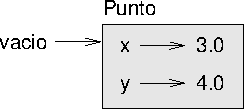
\includegraphics[scale=0.8]{figs/point.pdf}}
\caption{Object diagram.}
\label{fig.point}
\end{figure}

The variable {\tt blank} refers to a Point object, which
contains two attributes.  Each attribute refers to a
floating-point number.

You can read the value of an attribute using the same syntax:

\begin{verbatim}
>>> blank.y
4.0
>>> x = blank.x
>>> x
3.0
\end{verbatim}
%
The expression {\tt blank.x} means, ``Go to the object {\tt blank}
refers to and get the value of {\tt x}.''  In the example, we assign that
value to a variable named {\tt x}.  There is no conflict between
the variable {\tt x} and the attribute {\tt x}.

You can use dot notation as part of any expression.  For example:

\begin{verbatim}
>>> '(%g, %g)' % (blank.x, blank.y)
'(3.0, 4.0)'
>>> distance = math.sqrt(blank.x**2 + blank.y**2)
>>> distance
5.0
\end{verbatim}
%
You can pass an instance as an argument in the usual way.
For example:
\index{instance!as argument}

\begin{verbatim}
def print_point(p):
    print('(%g, %g)' % (p.x, p.y))
\end{verbatim}
%
\verb"print_point" takes a point as an argument and displays it in
mathematical notation.  To invoke it, you can pass {\tt blank} as
an argument:

\begin{verbatim}
>>> print_point(blank)
(3.0, 4.0)
\end{verbatim}
%
Inside the function, {\tt p} is an alias for {\tt blank}, so if
the function modifies {\tt p}, {\tt blank} changes.
\index{aliasing}

As an exercise, write a function called \verb"distance_between_points"
that takes two Points as arguments and returns the distance between
them.


\section{Rectangles}
\label{rectangles}

Sometimes it is obvious what the attributes of an object should be,
but other times you have to make decisions.  For example, imagine you
are designing a class to represent rectangles.  What attributes would
you use to specify the location and size of a rectangle?  You can
ignore angle; to keep things simple, assume that the rectangle is
either vertical or horizontal.
\index{representation}

There are at least two possibilities:

\begin{itemize}

\item You could specify one corner of the rectangle
(or the center), the width, and the height.

\item You could specify two opposing corners.

\end{itemize}

At this point it is hard to say whether either is better than
the other, so we'll implement the first one, just as an example.
\index{Rectangle class}
\index{class!Rectangle}

Here is the class definition:

\begin{verbatim}
class Rectangle:
    """Represents a rectangle.

    attributes: width, height, corner.
    """
\end{verbatim}
%
The docstring lists the attributes:  {\tt width} and
{\tt height} are numbers; {\tt corner} is a Point object that
specifies the lower-left corner.

To represent a rectangle, you have to instantiate a Rectangle
object and assign values to the attributes:

\begin{verbatim}
box = Rectangle()
box.width = 100.0
box.height = 200.0
box.corner = Point()
box.corner.x = 0.0
box.corner.y = 0.0
\end{verbatim}
%
The expression {\tt box.corner.x} means,
``Go to the object {\tt box} refers to and select the attribute named
{\tt corner}; then go to that object and select the attribute named
{\tt x}.''

\begin{figure}
\centerline
{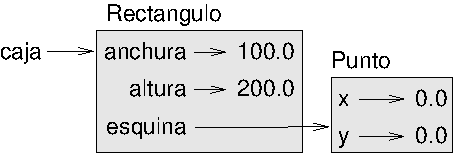
\includegraphics[scale=0.8]{figs/rectangle.pdf}}
\caption{Object diagram.}
\label{fig.rectangle}
\end{figure}


Figure~\ref{fig.rectangle} shows the state of this object.
An object that is an attribute of another object is {\bf embedded}.
\index{state diagram}
\index{diagram!state}
\index{object diagram}
\index{diagram!object}
\index{embedded object}
\index{object!embedded}


\section{Instances as return values}
\index{instance!as return value}
\index{return value}

Functions can return instances.  For example, \verb"find_center"
takes a {\tt Rectangle} as an argument and returns a {\tt Point}
that contains the coordinates of the center of the {\tt Rectangle}:

\begin{verbatim}
def find_center(rect):
    p = Point()
    p.x = rect.corner.x + rect.width/2
    p.y = rect.corner.y + rect.height/2
    return p
\end{verbatim}
%
Here is an example that passes {\tt box} as an argument and assigns
the resulting Point to {\tt center}:

\begin{verbatim}
>>> center = find_center(box)
>>> print_point(center)
(50, 100)
\end{verbatim}
%

\section{Objects are mutable}
\index{object!mutable}
\index{mutability}

You can change the state of an object by making an assignment to one of
its attributes.  For example, to change the size of a rectangle
without changing its position, you can modify the values of {\tt
width} and {\tt height}:

\begin{verbatim}
box.width = box.width + 50
box.height = box.height + 100
\end{verbatim}
%
You can also write functions that modify objects.  For example,
\verb"grow_rectangle" takes a Rectangle object and two numbers,
{\tt dwidth} and {\tt dheight}, and adds the numbers to the
width and height of the rectangle:

\begin{verbatim}
def grow_rectangle(rect, dwidth, dheight):
    rect.width += dwidth
    rect.height += dheight
\end{verbatim}
%
Here is an example that demonstrates the effect:

\begin{verbatim}
>>> box.width, box.height
(150.0, 300.0)
>>> grow_rectangle(box, 50, 100)
>>> box.width, box.height
(200.0, 400.0)
\end{verbatim}
%
Inside the function, {\tt rect} is an
alias for {\tt box}, so when the function modifies {\tt rect},
{\tt box} changes.

As an exercise, write a function named \verb"move_rectangle" that takes
a Rectangle and two numbers named {\tt dx} and {\tt dy}.  It
should change the location of the rectangle by adding {\tt dx}
to the {\tt x} coordinate of {\tt corner} and adding {\tt dy}
to the {\tt y} coordinate of {\tt corner}.


\section{Copying}
\label{copying}
\index{aliasing}

Aliasing can make a program difficult to read because changes
in one place might have unexpected effects in another place.
It is hard to keep track of all the variables that might refer
to a given object.
\index{copying objects}
\index{object!copying}
\index{copy module}
\index{module!copy}

Copying an object is often an alternative to aliasing.
The {\tt copy} module contains a function called {\tt copy} that
can duplicate any object:

\begin{verbatim}
>>> p1 = Point()
>>> p1.x = 3.0
>>> p1.y = 4.0

>>> import copy
>>> p2 = copy.copy(p1)
\end{verbatim}
%
{\tt p1} and {\tt p2} contain the same data, but they are
not the same Point.

\begin{verbatim}
>>> print_point(p1)
(3, 4)
>>> print_point(p2)
(3, 4)
>>> p1 is p2
False
>>> p1 == p2
False
\end{verbatim}
%
The {\tt is} operator indicates that {\tt p1} and {\tt p2} are not the
same object, which is what we expected.  But you might have expected
{\tt ==} to yield {\tt True} because these points contain the same
data.  In that case, you will be disappointed to learn that for
instances, the default behavior of the {\tt ==} operator is the same
as the {\tt is} operator; it checks object identity, not object
equivalence.  That's because for programmer-defined types, Python doesn't
know what should be considered equivalent.  At least, not yet.
\index{is operator}
\index{operator!is}
\index{identity}
\index{equivalence}

If you use {\tt copy.copy} to duplicate a Rectangle, you will find
that it copies the Rectangle object but not the embedded Point.
\index{embedded object!copying}

\begin{verbatim}
>>> box2 = copy.copy(box)
>>> box2 is box
False
>>> box2.corner is box.corner
True
\end{verbatim}

\begin{figure}
\centerline
{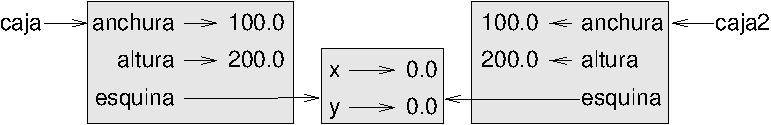
\includegraphics[scale=0.8]{figs/rectangle2.pdf}}
\caption{Object diagram.}
\label{fig.rectangle2}
\end{figure}

Figure~\ref{fig.rectangle2} shows what the object diagram looks like.
\index{state diagram}
\index{diagram!state}
\index{object diagram}
\index{diagram!object}
This operation is called a {\bf shallow copy} because it copies the
object and any references it contains, but not the embedded objects.
\index{shallow copy}
\index{copy!shallow}

For most applications, this is not what you want.  In this example,
invoking \verb"grow_rectangle" on one of the Rectangles would not
affect the other, but invoking \verb"move_rectangle" on either would
affect both!  This behavior is confusing and error-prone.
\index{deep copy}
\index{copy!deep}

Fortunately, the {\tt copy} module provides a method named {\tt
deepcopy} that copies not only the object but also
the objects it refers to, and the objects {\em they} refer to,
and so on.
You will not be surprised to learn that this operation is
called a {\bf deep copy}.
\index{deepcopy function}
\index{function!deepcopy}

\begin{verbatim}
>>> box3 = copy.deepcopy(box)
>>> box3 is box
False
>>> box3.corner is box.corner
False
\end{verbatim}
%
{\tt box3} and {\tt box} are completely separate objects.

As an exercise, write a version of \verb"move_rectangle" that creates and
returns a new Rectangle instead of modifying the old one.


\section{Debugging}
\label{hasattr}
\index{debugging}

When you start working with objects, you are likely to encounter
some new exceptions.  If you try to access an attribute
that doesn't exist, you get an {\tt AttributeError}:
\index{exception!AttributeError}
\index{AttributeError}

\begin{verbatim}
>>> p = Point()
>>> p.x = 3
>>> p.y = 4
>>> p.z
AttributeError: Point instance has no attribute 'z'
\end{verbatim}
%
If you are not sure what type an object is, you can ask:
\index{type function}
\index{function!type}

\begin{verbatim}
>>> type(p)
<class '__main__.Point'>
\end{verbatim}
%
You can also use {\tt isinstance} to check whether an object
is an instance of a class:
\index{isinstance function}
\index{function!isinstance}

\begin{verbatim}
>>> isinstance(p, Point)
True
\end{verbatim}
%
If you are not sure whether an object has a particular attribute,
you can use the built-in function {\tt hasattr}:
\index{hasattr function}
\index{function!hasattr}

\begin{verbatim}
>>> hasattr(p, 'x')
True
>>> hasattr(p, 'z')
False
\end{verbatim}
%
The first argument can be any object; the second argument is a {\em
string} that contains the name of the attribute.
\index{attribute}

You can also use a {\tt try} statement to see if the object has the
attributes you need:
\index{try statement}
\index{statement!try}

\begin{verbatim}
try:
    x = p.x
except AttributeError:
    x = 0
\end{verbatim}

This approach can make it easier to write functions that work with
different types; more on that topic is
coming up in Section~\ref{polymorphism}.


\section{Glossary}

\begin{description}

\item[class:] A programmer-defined type.  A class definition creates a new
class object.
\index{class}
\index{programmer-defined type}
\index{type!programmer-defined}

\item[class object:] An object that contains information about a
programmer-defined type.  The class object can be used to create instances
of the type.
\index{class object}
\index{object!class}

\item[instance:] An object that belongs to a class.
\index{instance}

\item[instantiate:] To create a new object.
\index{instantiate}

\item[attribute:] One of the named values associated with an object.
\index{attribute!instance}
\index{instance attribute}

\item[embedded object:] An object that is stored as an attribute
of another object.
\index{embedded object}
\index{object!embedded}

\item[shallow copy:] To copy the contents of an object, including
any references to embedded objects;
implemented by the {\tt copy} function in the {\tt copy} module.
\index{shallow copy}

\item[deep copy:] To copy the contents of an object as well as any
embedded objects, and any objects embedded in them, and so on;
implemented by the {\tt deepcopy} function in the {\tt copy} module.
\index{deep copy}

\item[object diagram:] A diagram that shows objects, their
attributes, and the values of the attributes.
\index{object diagram}
\index{diagram!object}

\end{description}


\section{Exercises}

\begin{exercise}

Write a definition for a class named {\tt Circle} with attributes
{\tt center} and {\tt radius}, where {\tt center} is a Point object
and radius is a number.

Instantiate a Circle object that represents a circle with its center
at $(150, 100)$ and radius 75.

Write a function named \verb"point_in_circle" that takes a Circle and
a Point and returns True if the Point lies in or on the boundary of
the circle.

Write a function named \verb"rect_in_circle" that takes a Circle and a
Rectangle and returns True if the Rectangle lies entirely in or on the boundary
of the circle.

Write a function named \verb"rect_circle_overlap" that takes a Circle
and a Rectangle and returns True if any of the corners of the Rectangle fall
inside the circle.  Or as a more challenging version, return True if
any part of the Rectangle falls inside the circle.

Solution: \url{http://thinkpython2.com/code/Circle.py}.

\end{exercise}


\begin{exercise}

Write a function called \verb"draw_rect" that takes a Turtle object
and a Rectangle and uses the Turtle to draw the Rectangle.  See
Chapter~\ref{turtlechap} for examples using Turtle objects.

Write a function called \verb"draw_circle" that takes a Turtle and
a Circle and draws the Circle.

Solution: \url{http://thinkpython2.com/code/draw.py}.

\end{exercise}



\chapter{Classes and functions}
\label{time}

Now that we know how to create new types, the next
step is to write functions that take programmer-defined objects
as parameters and return them as results.  In this chapter I
also present ``functional programming style'' and two new
program development plans.

Code examples from this chapter are available from
\url{http://thinkpython2.com/code/Time1.py}.
Solutions to the exercises are at
\url{http://thinkpython2.com/code/Time1_soln.py}.


\section{Time}
\label{isafter}

As another example of a programmer-defined type, we'll define a class
called {\tt Time} that records the time of day.  The class definition
looks like this: \index{programmer-defined type}
\index{type!programmer-defined} \index{Time class} \index{class!Time}

\begin{verbatim}
class Time:
    """Represents the time of day.

    attributes: hour, minute, second
    """
\end{verbatim}
%
We can create a new {\tt Time} object and assign
attributes for hours, minutes, and seconds:

\begin{verbatim}
time = Time()
time.hour = 11
time.minute = 59
time.second = 30
\end{verbatim}
%
The state diagram for the {\tt Time} object looks like Figure~\ref{fig.time}.
\index{state diagram}
\index{diagram!state}
\index{object diagram}
\index{diagram!object}

As an exercise, write a function called \verb"print_time" that takes a
Time object and prints it in the form {\tt hour:minute:second}.
Hint: the format sequence \verb"'%.2d'" prints an integer using
at least two digits, including a leading zero if necessary.

Write a boolean function called \verb"is_after" that
takes two Time objects, {\tt t1} and {\tt t2}, and
returns {\tt True} if {\tt t1} follows {\tt t2} chronologically and
{\tt False} otherwise.  Challenge: don't use an {\tt if} statement.

\begin{figure}
\centerline
{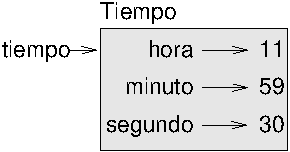
\includegraphics[scale=0.8]{figs/time.pdf}}
\caption{Object diagram.}
\label{fig.time}
\end{figure}


\section{Pure functions}
\index{prototype and patch}
\index{development plan!prototype and patch}

In the next few sections, we'll write two functions that add time
values.  They demonstrate two kinds of functions: pure functions and
modifiers.  They also demonstrate a development plan I'll call {\bf
  prototype and patch}, which is a way of tackling a complex problem
by starting with a simple prototype and incrementally dealing with the
complications.

Here is a simple prototype of \verb"add_time":

\begin{verbatim}
def add_time(t1, t2):
    sum = Time()
    sum.hour = t1.hour + t2.hour
    sum.minute = t1.minute + t2.minute
    sum.second = t1.second + t2.second
    return sum
\end{verbatim}
%
The function creates a new {\tt Time} object, initializes its
attributes, and returns a reference to the new object.  This is called
a {\bf pure function} because it does not modify any of the objects
passed to it as arguments and it has no effect,
like displaying a value or getting user input,
other than returning a value.
\index{pure function}
\index{function type!pure}

To test this function, I'll create two Time objects: {\tt start}
contains the start time of a movie, like {\em Monty Python and the
Holy Grail}, and {\tt duration} contains the run time of the movie,
which is one hour 35 minutes.
\index{Monty Python and the Holy Grail}

\verb"add_time" figures out when the movie will be done.

\begin{verbatim}
>>> start = Time()
>>> start.hour = 9
>>> start.minute = 45
>>> start.second =  0

>>> duration = Time()
>>> duration.hour = 1
>>> duration.minute = 35
>>> duration.second = 0

>>> done = add_time(start, duration)
>>> print_time(done)
10:80:00
\end{verbatim}
%
The result, {\tt 10:80:00} might not be what you were hoping
for.  The problem is that this function does not deal with cases where the
number of seconds or minutes adds up to more than sixty.  When that
happens, we have to ``carry'' the extra seconds into the minute column
or the extra minutes into the hour column.
\index{carrying, addition with}

Here's an improved version:

\begin{verbatim}
def add_time(t1, t2):
    sum = Time()
    sum.hour = t1.hour + t2.hour
    sum.minute = t1.minute + t2.minute
    sum.second = t1.second + t2.second

    if sum.second >= 60:
        sum.second -= 60
        sum.minute += 1

    if sum.minute >= 60:
        sum.minute -= 60
        sum.hour += 1

    return sum
\end{verbatim}
%
Although this function is correct, it is starting to get big.
We will see a shorter alternative later.


\section{Modifiers}
\label{increment}
\index{modifier}
\index{function type!modifier}

Sometimes it is useful for a function to modify the objects it gets as
parameters.  In that case, the changes are visible to the caller.
Functions that work this way are called {\bf modifiers}.
\index{increment}

{\tt increment}, which adds a given number of seconds to a {\tt Time}
object, can be written naturally as a
modifier.  Here is a rough draft:

\begin{verbatim}
def increment(time, seconds):
    time.second += seconds

    if time.second >= 60:
        time.second -= 60
        time.minute += 1

    if time.minute >= 60:
        time.minute -= 60
        time.hour += 1
\end{verbatim}
%
The first line performs the basic operation; the remainder deals
with the special cases we saw before.
\index{special case}

Is this function correct?  What happens if {\tt seconds}
is much greater than sixty?

In that case, it is not enough to carry once; we have to keep doing it
until {\tt time.second} is less than sixty.  One solution is to
replace the {\tt if} statements with {\tt while} statements.  That
would make the function correct, but not very efficient.  As an
exercise, write a correct version of {\tt increment} that doesn't
contain any loops.

Anything that can be done with modifiers can also be done with pure
functions.  In fact, some programming languages only allow pure
functions.  There is some evidence that programs that use pure
functions are faster to develop and less error-prone than programs
that use modifiers.  But modifiers are convenient at times,
and functional programs tend to be less efficient.

In general, I recommend that you write pure functions whenever it is
reasonable and resort to modifiers only if there is a compelling
advantage.  This approach might be called a {\bf functional
programming style}.
\index{functional programming style}

As an exercise, write a ``pure'' version of {\tt increment} that
creates and returns a new Time object rather than modifying the
parameter.


\section{Prototyping versus planning}
\label{prototype}
\index{prototype and patch}
\index{development plan!prototype and patch}
\index{planned development}
\index{development plan!designed}

The development plan I am demonstrating is called ``prototype and
patch''.  For each function, I wrote a prototype that performed the
basic calculation and then tested it, patching errors along the
way.

This approach can be effective, especially if you don't yet have a
deep understanding of the problem.  But incremental corrections can
generate code that is unnecessarily complicated---since it deals with
many special cases---and unreliable---since it is hard to know if you
have found all the errors.

An alternative is {\bf designed development}, in which high-level
insight into the problem can make the programming much easier.  In
this case, the insight is that a Time object is really a three-digit
number in base 60 (see \url{http://en.wikipedia.org/wiki/Sexagesimal}.)!  The
{\tt second} attribute is the ``ones column'', the {\tt minute}
attribute is the ``sixties column'', and the {\tt hour} attribute is
the ``thirty-six hundreds column''.
\index{sexagesimal}

When we wrote \verb"add_time" and {\tt increment}, we were effectively
doing addition in base 60, which is why we had to carry from one
column to the next.
\index{carrying, addition with}

This observation suggests another approach to the whole problem---we
can convert Time objects to integers and take advantage of the fact
that the computer knows how to do integer arithmetic.

Here is a function that converts Times to integers:

\begin{verbatim}
def time_to_int(time):
    minutes = time.hour * 60 + time.minute
    seconds = minutes * 60 + time.second
    return seconds
\end{verbatim}
%
And here is a function that converts an integer to a Time
(recall that {\tt divmod} divides the first argument by the second
and returns the quotient and remainder as a tuple).
\index{divmod}

\begin{verbatim}
def int_to_time(seconds):
    time = Time()
    minutes, time.second = divmod(seconds, 60)
    time.hour, time.minute = divmod(minutes, 60)
    return time
\end{verbatim}
%
You might have to think a bit, and run some tests, to convince
yourself that these functions are correct.  One way to test them is to
check that \verb"time_to_int(int_to_time(x)) == x" for many values of
{\tt x}.  This is an example of a consistency check.
\index{consistency check}

Once you are convinced they are correct, you can use them to
rewrite \verb"add_time":

\begin{verbatim}
def add_time(t1, t2):
    seconds = time_to_int(t1) + time_to_int(t2)
    return int_to_time(seconds)
\end{verbatim}
%
This version is shorter than the original, and easier to verify.  As
an exercise, rewrite {\tt increment} using \verb"time_to_int" and
\verb"int_to_time".

In some ways, converting from base 60 to base 10 and back is harder
than just dealing with times.  Base conversion is more abstract; our
intuition for dealing with time values is better.

But if we have the insight to treat times as base 60 numbers and make
the investment of writing the conversion functions (\verb"time_to_int"
and \verb"int_to_time"), we get a program that is shorter, easier to
read and debug, and more reliable.

It is also easier to add features later.  For example, imagine
subtracting two Times to find the duration between them.  The
naive approach would be to implement subtraction with borrowing.
Using the conversion functions would be easier and more likely to be
correct.
\index{subtraction with borrowing}
\index{borrowing, subtraction with}
\index{generalization}

Ironically, sometimes making a problem harder (or more general) makes it
easier (because there are fewer special cases and fewer opportunities
for error).


\section{Debugging}
\index{debugging}

A Time object is well-formed if the values of {\tt minute} and {\tt
second} are between 0 and 60 (including 0 but not 60) and if
{\tt hour} is positive.  {\tt hour} and {\tt minute} should be
integral values, but we might allow {\tt second} to have a
fraction part.
\index{invariant}

Requirements like these are called {\bf invariants} because
they should always be true.  To put it a different way, if they
are not true, something has gone wrong.

Writing code to check invariants can help detect errors
and find their causes.  For example, you might have a function
like \verb"valid_time" that takes a Time object and returns
{\tt False} if it violates an invariant:

\begin{verbatim}
def valid_time(time):
    if time.hour < 0 or time.minute < 0 or time.second < 0:
        return False
    if time.minute >= 60 or time.second >= 60:
        return False
    return True
\end{verbatim}
%
At the beginning of each function you could check the
arguments to make sure they are valid:
\index{raise statement}
\index{statement!raise}

\begin{verbatim}
def add_time(t1, t2):
    if not valid_time(t1) or not valid_time(t2):
        raise ValueError('invalid Time object in add_time')
    seconds = time_to_int(t1) + time_to_int(t2)
    return int_to_time(seconds)
\end{verbatim}
%
Or you could use an {\bf assert statement}, which checks a given invariant
and raises an exception if it fails:
\index{assert statement}
\index{statement!assert}

\begin{verbatim}
def add_time(t1, t2):
    assert valid_time(t1) and valid_time(t2)
    seconds = time_to_int(t1) + time_to_int(t2)
    return int_to_time(seconds)
\end{verbatim}
%
{\tt assert} statements are useful because they distinguish
code that deals with normal conditions from code
that checks for errors.


\section{Glossary}

\begin{description}

\item[prototype and patch:] A development plan that involves
writing a rough draft of a program, testing, and correcting errors as
they are found.
\index{prototype and patch}

\item[designed development:] A development plan that involves
high-level insight into the problem and more planning than incremental
development or prototype development.
\index{designed development}

\item[pure function:] A function that does not modify any of the objects it
receives as arguments.  Most pure functions are fruitful.
\index{pure function}

\item[modifier:] A function that changes one or more of the objects it
  receives as arguments.  Most modifiers are void; that is, they
  return {\tt None}.  \index{modifier}

\item[functional programming style:] A style of program design in which the
majority of functions are pure.
\index{functional programming style}

\item[invariant:] A condition that should always be true during the
execution of a program.
\index{invariant}

\item[assert statement:] A statement that check a condition and raises
an exception if it fails.
\index{assert statement}
\index{statement!assert}

\end{description}


\section{Exercises}

Code examples from this chapter are available from
\url{http://thinkpython2.com/code/Time1.py}; solutions to the
exercises are available from \url{http://thinkpython2.com/code/Time1_soln.py}.

\begin{exercise}

Write a function called \verb"mul_time" that takes a Time object
and a number and returns a new Time object that contains
the product of the original Time and the number.

Then use \verb"mul_time" to write a function that takes a Time
object that represents the finishing time in a race, and a number
that represents the distance, and returns a Time object that represents
the average pace (time per mile).
\index{running pace}

\end{exercise}


\begin{exercise}
\index{datetime module}
\index{module!datetime}

The {\tt datetime} module provides {\tt time} objects
that are similar to the Time objects in this chapter, but
they provide a rich set of methods and operators.  Read the
documentation at \url{http://docs.python.org/3/library/datetime.html}.

\begin{enumerate}

\item Use the {\tt datetime} module to write a program that gets the
  current date and prints the day of the week.

\item Write a program that takes a birthday as input and prints the
  user's age and the number of days, hours, minutes and seconds until
  their next birthday.
\index{birthday}

\item For two people born on different days, there is a day when one
  is twice as old as the other.  That's their Double Day.  Write a
  program that takes two birth dates and computes their Double Day.

\item For a little more challenge, write the more general version that
  computes the day when one person is $n$ times older than the other.
\index{Double Day}

\end{enumerate}

Solution: \url{http://thinkpython2.com/code/double.py}

\end{exercise}


\chapter{Classes and methods}

Although we are using some of Python's object-oriented features,
the programs from the last two chapters are not really
object-oriented because they don't represent the relationships
between programmer-defined types and the functions that operate
on them.  The next step is to transform those functions into
methods that make the relationships explicit.

Code examples from this chapter are available from
\url{http://thinkpython2.com/code/Time2.py}, and solutions
to the exercises are in \url{http://thinkpython2.com/code/Point2_soln.py}.


\section{Object-oriented features}
\index{object-oriented programming}

Python is an {\bf object-oriented programming language}, which means
that it provides features that support object-oriented
programming, which has these defining characteristics:

\begin{itemize}

\item Programs include class and method definitions.

\item Most of the computation is expressed in terms of operations on
  objects.

\item Objects often represent things
in the real world, and methods often
correspond to the ways things in the real world interact.

\end{itemize}

For example, the {\tt Time} class defined in Chapter~\ref{time}
corresponds to the way people record the time of day, and the
functions we defined correspond to the kinds of things people do with
times.  Similarly, the {\tt Point} and {\tt Rectangle} classes
in Chapter~\ref{clobjects}
correspond to the mathematical concepts of a point and a rectangle.

So far, we have not taken advantage of the features Python provides to
support object-oriented programming.  These
features are not strictly necessary; most of them provide
alternative syntax for things we have already done.  But in many cases,
the alternative is more concise and more accurately conveys the
structure of the program.

For example, in {\tt Time1.py} there is no obvious
connection between the class definition and the function definitions
that follow.  With some examination, it is apparent that every function
takes at least one {\tt Time} object as an argument.
\index{method}
\index{function}

This observation is the motivation for {\bf methods}; a method is
a function that is associated with a particular class.
We have seen methods for strings, lists, dictionaries and tuples.
In this chapter, we will define methods for programmer-defined types.
\index{syntax}
\index{semantics}
\index{programmer-defined type}
\index{type!programmer-defined}

Methods are semantically the same as functions, but there are
two syntactic differences:

\begin{itemize}

\item Methods are defined inside a class definition in order
to make the relationship between the class and the method explicit.

\item The syntax for invoking a method is different from the
syntax for calling a function.

\end{itemize}

In the next few sections, we will take the functions from the previous
two chapters and transform them into methods.  This transformation is
purely mechanical; you can do it by following a sequence of
steps.  If you are comfortable converting from one form to another,
you will be able to choose the best form for whatever you are doing.


\section{Printing objects}
\index{object!printing}

In Chapter~\ref{time}, we defined a class named
{\tt Time} and in Section~\ref{isafter}, you
wrote a function named \verb"print_time":

\begin{verbatim}
class Time:
    """Represents the time of day."""

def print_time(time):
    print('%.2d:%.2d:%.2d' % (time.hour, time.minute, time.second))
\end{verbatim}
%
To call this function, you have to pass a {\tt Time} object as an
argument:

\begin{verbatim}
>>> start = Time()
>>> start.hour = 9
>>> start.minute = 45
>>> start.second = 00
>>> print_time(start)
09:45:00
\end{verbatim}
%
To make \verb"print_time" a method, all we have to do is
move the function definition inside the class definition.  Notice
the change in indentation.
\index{indentation}

\begin{verbatim}
class Time:
    def print_time(time):
        print('%.2d:%.2d:%.2d' % (time.hour, time.minute, time.second))
\end{verbatim}
%
Now there are two ways to call \verb"print_time".  The first
(and less common) way is to use function syntax:
\index{function syntax}
\index{dot notation}

\begin{verbatim}
>>> Time.print_time(start)
09:45:00
\end{verbatim}
%
In this use of dot notation, {\tt Time} is the name of the class,
and \verb"print_time" is the name of the method.  {\tt start} is
passed as a parameter.

The second (and more concise) way is to use method syntax:
\index{method syntax}

\begin{verbatim}
>>> start.print_time()
09:45:00
\end{verbatim}
%
In this use of dot notation, \verb"print_time" is the name of the
method (again), and {\tt start} is the object the method is
invoked on, which is called the {\bf subject}.  Just as the
subject of a sentence is what the sentence is about, the subject
of a method invocation is what the method is about.
\index{subject}

Inside the method, the subject is assigned to the first
parameter, so in this case {\tt start} is assigned
to {\tt time}.
\index{self (parameter name)}
\index{parameter!self}

By convention, the first parameter of a method is
called {\tt self}, so it would be more common to write
\verb"print_time" like this:

\begin{verbatim}
class Time:
    def print_time(self):
        print('%.2d:%.2d:%.2d' % (self.hour, self.minute, self.second))
\end{verbatim}
%
The reason for this convention is an implicit metaphor:
\index{metaphor, method invocation}

\begin{itemize}

\item The syntax for a function call, \verb"print_time(start)",
  suggests that the function is the active agent.  It says something
  like, ``Hey \verb"print_time"!  Here's an object for you to print.''

\item In object-oriented programming, the objects are the active
  agents.  A method invocation like \verb"start.print_time()" says
  ``Hey {\tt start}!  Please print yourself.''

\end{itemize}

This change in perspective might be more polite, but it is not obvious
that it is useful.  In the examples we have seen so far, it may not
be.  But sometimes shifting responsibility from the functions onto the
objects makes it possible to write more versatile functions (or
methods), and makes it easier to maintain and reuse code.

As an exercise, rewrite \verb"time_to_int" (from
Section~\ref{prototype}) as a method.  You might be tempted to
rewrite \verb"int_to_time" as a method, too, but that doesn't
really make sense because there would be no object to invoke
it on.


\section{Another example}
\index{increment}

Here's a version of {\tt increment} (from Section~\ref{increment})
rewritten as a method:

\begin{verbatim}
# inside class Time:

    def increment(self, seconds):
        seconds += self.time_to_int()
        return int_to_time(seconds)
\end{verbatim}
%
This version assumes that \verb"time_to_int" is written
as a method.  Also, note that
it is a pure function, not a modifier.

Here's how you would invoke {\tt increment}:

\begin{verbatim}
>>> start.print_time()
09:45:00
>>> end = start.increment(1337)
>>> end.print_time()
10:07:17
\end{verbatim}
%
The subject, {\tt start}, gets assigned to the first parameter,
{\tt self}.  The argument, {\tt 1337}, gets assigned to the
second parameter, {\tt seconds}.

This mechanism can be confusing, especially if you make an error.
For example, if you invoke {\tt increment} with two arguments, you
get:
\index{exception!TypeError}
\index{TypeError}

\begin{verbatim}
>>> end = start.increment(1337, 460)
TypeError: increment() takes 2 positional arguments but 3 were given
\end{verbatim}
%
The error message is initially confusing, because there are
only two arguments in parentheses.  But the subject is also
considered an argument, so all together that's three.

By the way, a {\bf positional argument} is an argument that
doesn't have a parameter name; that is, it is not a keyword
argument.  In this function call:
\index{positional argument}
\index{argument!positional}

\begin{verbatim}
sketch(parrot, cage, dead=True)
\end{verbatim}

{\tt parrot} and {\tt cage} are positional, and {\tt dead} is
a keyword argument.


\section{A more complicated example}

Rewriting \verb"is_after" (from Section~\ref{isafter}) is slightly
more complicated because it takes two Time objects as parameters.  In
this case it is conventional to name the first parameter {\tt self}
and the second parameter {\tt other}: \index{other (parameter name)}
\index{parameter!other}

\begin{verbatim}
# inside class Time:

    def is_after(self, other):
        return self.time_to_int() > other.time_to_int()
\end{verbatim}
%
To use this method, you have to invoke it on one object and pass
the other as an argument:

\begin{verbatim}
>>> end.is_after(start)
True
\end{verbatim}
%
One nice thing about this syntax is that it almost reads
like English: ``end is after start?''


\section{The init method}
\index{init method}
\index{method!init}

The init method (short for ``initialization'') is
a special method that gets invoked when an object is instantiated.
Its full name is \verb"__init__" (two underscore characters,
followed by {\tt init}, and then two more underscores).  An
init method for the {\tt Time} class might look like this:

\begin{verbatim}
# inside class Time:

    def __init__(self, hour=0, minute=0, second=0):
        self.hour = hour
        self.minute = minute
        self.second = second
\end{verbatim}
%
It is common for the parameters of \verb"__init__"
to have the same names as the attributes.  The statement

\begin{verbatim}
        self.hour = hour
\end{verbatim}
%
stores the value of the parameter {\tt hour} as an attribute
of {\tt self}.
\index{optional parameter}
\index{parameter!optional}
\index{default value}
\index{override}

The parameters are optional, so if you call {\tt Time} with
no arguments, you get the default values.

\begin{verbatim}
>>> time = Time()
>>> time.print_time()
00:00:00
\end{verbatim}
%
If you provide one argument, it overrides {\tt hour}:

\begin{verbatim}
>>> time = Time (9)
>>> time.print_time()
09:00:00
\end{verbatim}
%
If you provide two arguments, they override {\tt hour} and
{\tt minute}.

\begin{verbatim}
>>> time = Time(9, 45)
>>> time.print_time()
09:45:00
\end{verbatim}
%
And if you provide three arguments, they override all three
default values.

As an exercise, write an init method for the {\tt Point} class that takes
{\tt x} and {\tt y} as optional parameters and assigns
them to the corresponding attributes.
\index{Point class}
\index{class!Point}


\section{The {\tt \_\_str\_\_} method}
\index{str method@\_\_str\_\_ method}
\index{method!\_\_str\_\_}

\verb"__str__" is a special method, like \verb"__init__",
that is supposed to return a string representation of an object.
\index{string representation}

For example, here is a {\tt str} method for Time objects:

\begin{verbatim}
# inside class Time:

    def __str__(self):
        return '%.2d:%.2d:%.2d' % (self.hour, self.minute, self.second)
\end{verbatim}
%
When you {\tt print} an object, Python invokes the {\tt str} method:
\index{print statement}
\index{statement!print}

\begin{verbatim}
>>> time = Time(9, 45)
>>> print(time)
09:45:00
\end{verbatim}
%
When I write a new class, I almost always start by writing
\verb"__init__", which makes it easier to instantiate objects, and
\verb"__str__", which is useful for debugging.

As an exercise, write a {\tt str} method for the {\tt Point} class.
Create a Point object and print it.


\section{Operator overloading}
\label{operator.overloading}

By defining other special methods, you can specify the behavior
of operators on programmer-defined types.  For example, if you define
a method named \verb"__add__" for the {\tt Time} class, you can use the
{\tt +} operator on Time objects.
\index{programmer-defined type}
\index{type!programmer-defined}

Here is what the definition might look like:
\index{add method}
\index{method!add}

\begin{verbatim}
# inside class Time:

    def __add__(self, other):
        seconds = self.time_to_int() + other.time_to_int()
        return int_to_time(seconds)
\end{verbatim}
%
And here is how you could use it:

\begin{verbatim}
>>> start = Time(9, 45)
>>> duration = Time(1, 35)
>>> print(start + duration)
11:20:00
\end{verbatim}
%
When you apply the {\tt +} operator to Time objects, Python invokes
\verb"__add__".  When you print the result, Python invokes
\verb"__str__".  So there is a lot happening behind the scenes!
\index{operator overloading}

Changing the behavior of an operator so that it works with
programmer-defined types is called {\bf operator overloading}.  For every
operator in Python there is a corresponding special method, like
\verb"__add__".  For more details, see
\url{http://docs.python.org/3/reference/datamodel.html#specialnames}.

As an exercise, write an {\tt add} method for the Point class.


\section{Type-based dispatch}

In the previous section we added two Time objects, but you
also might want to add an integer to a Time object.  The
following is a version of \verb"__add__"
that checks the type of {\tt other} and invokes either
\verb"add_time" or {\tt increment}:

\begin{verbatim}
# inside class Time:

    def __add__(self, other):
        if isinstance(other, Time):
            return self.add_time(other)
        else:
            return self.increment(other)

    def add_time(self, other):
        seconds = self.time_to_int() + other.time_to_int()
        return int_to_time(seconds)

    def increment(self, seconds):
        seconds += self.time_to_int()
        return int_to_time(seconds)
\end{verbatim}
%
The built-in function {\tt isinstance} takes a value and a
class object, and returns {\tt True} if the value is an instance
of the class.
\index{isinstance function}
\index{function!isinstance}

If {\tt other} is a Time object, \verb"__add__" invokes
\verb"add_time".  Otherwise it assumes that the parameter
is a number and invokes {\tt increment}.  This operation is
called a {\bf type-based dispatch} because it dispatches the
computation to different methods based on the type of the
arguments.
\index{type-based dispatch}
\index{dispatch, type-based}

Here are examples that use the {\tt +} operator with different
types:

\begin{verbatim}
>>> start = Time(9, 45)
>>> duration = Time(1, 35)
>>> print(start + duration)
11:20:00
>>> print(start + 1337)
10:07:17
\end{verbatim}
%
Unfortunately, this implementation of addition is not commutative.
If the integer is the first operand, you get
\index{commutativity}

\begin{verbatim}
>>> print(1337 + start)
TypeError: unsupported operand type(s) for +: 'int' and 'instance'
\end{verbatim}
%
The problem is, instead of asking the Time object to add an integer,
Python is asking an integer to add a Time object, and it doesn't know
how.  But there is a clever solution for this problem: the
special method \verb"__radd__", which stands for ``right-side add''.
This method is invoked when a Time object appears on the right side of
the {\tt +} operator.  Here's the definition:
\index{radd method}
\index{method!radd}

\begin{verbatim}
# inside class Time:

    def __radd__(self, other):
        return self.__add__(other)
\end{verbatim}
%
And here's how it's used:

\begin{verbatim}
>>> print(1337 + start)
10:07:17
\end{verbatim}
%

As an exercise, write an {\tt add} method for Points that works with
either a Point object or a tuple:

\begin{itemize}

\item If the second operand is a Point, the method should return a new
Point whose $x$ coordinate is the sum of the $x$ coordinates of the
operands, and likewise for the $y$ coordinates.

\item If the second operand is a tuple, the method should add the
first element of the tuple to the $x$ coordinate and the second
element to the $y$ coordinate, and return a new Point with the result.

\end{itemize}




\section{Polymorphism}
\label{polymorphism}

Type-based dispatch is useful when it is necessary, but (fortunately)
it is not always necessary.  Often you can avoid it by writing functions
that work correctly for arguments with different types.
\index{type-based dispatch}
\index{dispatch!type-based}

Many of the functions we wrote for strings also
work for other sequence types.
For example, in Section~\ref{histogram}
we used {\tt histogram} to count the number of times each letter
appears in a word.

\begin{verbatim}
def histogram(s):
    d = dict()
    for c in s:
        if c not in d:
            d[c] = 1
        else:
            d[c] = d[c]+1
    return d
\end{verbatim}
%
This function also works for lists, tuples, and even dictionaries,
as long as the elements of {\tt s} are hashable, so they can be used
as keys in {\tt d}.

\begin{verbatim}
>>> t = ['spam', 'egg', 'spam', 'spam', 'bacon', 'spam']
>>> histogram(t)
{'bacon': 1, 'egg': 1, 'spam': 4}
\end{verbatim}
%
Functions that work with several types are called {\bf polymorphic}.
Polymorphism can facilitate code reuse.  For example, the built-in
function {\tt sum}, which adds the elements of a sequence, works
as long as the elements of the sequence support addition.
\index{polymorphism}

Since Time objects provide an {\tt add} method, they work
with {\tt sum}:

\begin{verbatim}
>>> t1 = Time(7, 43)
>>> t2 = Time(7, 41)
>>> t3 = Time(7, 37)
>>> total = sum([t1, t2, t3])
>>> print(total)
23:01:00
\end{verbatim}
%
In general, if all of the operations inside a function
work with a given type, the function works with that type.

The best kind of polymorphism is the unintentional kind, where
you discover that a function you already wrote can be
applied to a type you never planned for.


\section{Debugging}
\index{debugging}

It is legal to add attributes to objects at any point in the execution
of a program, but if you have objects with the same type that don't
have the same attributes, it is easy to make mistakes.
It is considered a good idea to
initialize all of an object's attributes in the init method.
\index{init method}
\index{attribute!initializing}

If you are not sure whether an object has a particular attribute, you
can use the built-in function {\tt hasattr} (see Section~\ref{hasattr}).
\index{hasattr function}
\index{function!hasattr}
\index{dict attribute@\_\_dict\_\_ attribute}
\index{attribute!\_\_dict\_\_}

Another way to access attributes is the built-in function {\tt vars},
which takes an object and returns a dictionary that maps from
attribute names (as strings) to their values:

\begin{verbatim}
>>> p = Point(3, 4)
>>> vars(p)
{'y': 4, 'x': 3}
\end{verbatim}
%
For purposes of debugging, you might find it useful to keep this
function handy:

\begin{verbatim}
def print_attributes(obj):
    for attr in vars(obj):
        print(attr, getattr(obj, attr))
\end{verbatim}
%
\verb"print_attributes" traverses the dictionary
and prints each attribute name and its corresponding value.
\index{traversal!dictionary}
\index{dictionary!traversal}

The built-in function {\tt getattr} takes an object and an attribute
name (as a string) and returns the attribute's value.
\index{getattr function}
\index{function!getattr}


\section{Interface and implementation}

One of the goals of object-oriented design is to make software more
maintainable, which means that you can keep the program working when
other parts of the system change, and modify the program to meet new
requirements.
\index{interface}
\index{implementation}
\index{maintainable}
\index{object-oriented design}

A design principle that helps achieve that goal is to keep
interfaces separate from implementations.  For objects, that means
that the methods a class provides should not depend on how the
attributes are represented.
\index{attribute}

For example, in this chapter we developed a class that represents
a time of day.  Methods provided by this class include
\verb"time_to_int", \verb"is_after", and \verb"add_time".

We could implement those methods in several ways.  The details of the
implementation depend on how we represent time.  In this chapter, the
attributes of a {\tt Time} object are {\tt hour}, {\tt minute}, and
{\tt second}.

As an alternative, we could replace these attributes with
a single integer representing the number of seconds
since midnight.  This implementation would make some methods,
like \verb"is_after", easier to write, but it makes other methods
harder.

After you deploy a new class, you might discover a better
implementation.  If other parts of the program are using your
class, it might be time-consuming and error-prone to change the
interface.

But if you designed the interface carefully, you can
change the implementation without changing the interface, which
means that other parts of the program don't have to change.


\section{Glossary}

\begin{description}

\item[object-oriented language:] A language that provides features,
  such as programmer-defined types and methods, that facilitate
  object-oriented programming.
\index{object-oriented language}

\item[object-oriented programming:] A style of programming in which
data and the operations that manipulate it are organized into classes
and methods.
\index{object-oriented programming}

\item[method:] A function that is defined inside a class definition and
is invoked on instances of that class.
\index{method}

\item[subject:] The object a method is invoked on.
\index{subject}

\item[positional argument:]  An argument that does not include
a parameter name, so it is not a keyword argument.
\index{positional argument}
\index{argument!positional}

\item[operator overloading:] Changing the behavior of an operator like
{\tt +} so it works with a programmer-defined type.
\index{overloading}
\index{operator!overloading}

\item[type-based dispatch:] A programming pattern that checks the type
of an operand and invokes different functions for different types.
\index{type-based dispatch}

\item[polymorphic:] Pertaining to a function that can work with more
  than one type.
\index{polymorphism}

\end{description}


\section{Exercises}

\begin{exercise}

Download the code from this chapter from
\url{http://thinkpython2.com/code/Time2.py}.  Change the attributes of
    {\tt Time} to be a single integer representing seconds since
    midnight.  Then modify the methods (and the function
    \verb"int_to_time") to work with the new implementation.  You
    should not have to modify the test code in {\tt main}.  When you
    are done, the output should be the same as before.  Solution:
    \url{http://thinkpython2.com/code/Time2_soln.py}.

\end{exercise}


\begin{exercise}
\label{kangaroo}
\index{default value!avoiding mutable}
\index{mutable object, as default value}
\index{worst bug}
\index{bug!worst}
\index{Kangaroo class}
\index{class!Kangaroo}

This exercise is a cautionary tale about one of the most
common, and difficult to find, errors in Python.
Write a definition for a class named {\tt Kangaroo} with the following
methods:

\begin{enumerate}

\item An \verb"__init__" method that initializes an attribute named
\verb"pouch_contents" to an empty list.

\item A method named \verb"put_in_pouch" that takes an object
of any type and adds it to \verb"pouch_contents".

\item A \verb"__str__" method that returns a string representation
of the Kangaroo object and the contents of the pouch.

\end{enumerate}
%
Test your code
by creating two {\tt Kangaroo} objects, assigning them to variables
named {\tt kanga} and {\tt roo}, and then adding {\tt roo} to the
contents of {\tt kanga}'s pouch.

Download \url{http://thinkpython2.com/code/BadKangaroo.py}.  It contains
a solution to the previous problem with one big, nasty bug.
Find and fix the bug.

If you get stuck, you can download
\url{http://thinkpython2.com/code/GoodKangaroo.py}, which explains the
problem and demonstrates a solution.
\index{aliasing}
\index{embedded object}
\index{object!embedded}

\end{exercise}



\chapter{Inheritance}

The language feature most often associated with object-oriented
programming is {\bf inheritance}.  Inheritance is the ability to
define a new class that is a modified version of an existing class.
In this chapter I demonstrate inheritance using classes that represent
playing cards, decks of cards, and poker hands.
\index{deck}
\index{card, playing}
\index{poker}

If you don't play
poker, you can read about it at
\url{http://en.wikipedia.org/wiki/Poker}, but you don't have to; I'll
tell you what you need to know for the exercises.

Code examples from
this chapter are available from
\url{http://thinkpython2.com/code/Card.py}.


\section{Card objects}

There are fifty-two cards in a deck, each of which belongs to one of
four suits and one of thirteen ranks.  The suits are Spades, Hearts,
Diamonds, and Clubs (in descending order in bridge).  The ranks are
Ace, 2, 3, 4, 5, 6, 7, 8, 9, 10, Jack, Queen, and King.  Depending on
the game that you are playing, an Ace may be higher than King
or lower than 2.
\index{rank}
\index{suit}

If we want to define a new object to represent a playing card, it is
obvious what the attributes should be: {\tt rank} and
{\tt suit}.  It is not as obvious what type the attributes
should be.  One possibility is to use strings containing words like
\verb"'Spade'" for suits and \verb"'Queen'" for ranks.  One problem with
this implementation is that it would not be easy to compare cards to
see which had a higher rank or suit.
\index{encode}
\index{encrypt}
\index{map to}
\index{representation}

An alternative is to use integers to {\bf encode} the ranks and suits.
In this context, ``encode'' means that we are going to define a mapping
between numbers and suits, or between numbers and ranks.  This
kind of encoding is not meant to be a secret (that
would be ``encryption'').

\newcommand{\mymapsto}{$\mapsto$}

For example, this table shows the suits and the corresponding integer
codes:

\begin{tabular}{l c l}
Spades & \mymapsto & 3 \\
Hearts & \mymapsto & 2 \\
Diamonds & \mymapsto & 1 \\
Clubs & \mymapsto & 0
\end{tabular}

This code makes it easy to compare cards; because higher suits map to
higher numbers, we can compare suits by comparing their codes.

The mapping for ranks is fairly obvious; each of the numerical ranks
maps to the corresponding integer, and for face cards:

\begin{tabular}{l c l}
Jack & \mymapsto & 11 \\
Queen & \mymapsto & 12 \\
King & \mymapsto & 13 \\
\end{tabular}

I am using the \mymapsto~symbol to make it clear that these mappings
are not part of the Python program.  They are part of the program
design, but they don't appear explicitly in the code.
\index{Card class}
\index{class!Card}

The class definition for {\tt Card} looks like this:

\begin{verbatim}
class Card:
    """Represents a standard playing card."""

    def __init__(self, suit=0, rank=2):
        self.suit = suit
        self.rank = rank
\end{verbatim}
%
As usual, the init method takes an optional
parameter for each attribute.  The default card is
the 2 of Clubs.
\index{init method}
\index{method!init}

To create a Card, you call {\tt Card} with the
suit and rank of the card you want.

\begin{verbatim}
queen_of_diamonds = Card(1, 12)
\end{verbatim}
%


\section{Class attributes}
\label{class.attribute}
\index{class attribute}
\index{attribute!class}

In order to print Card objects in a way that people can easily
read, we need a mapping from the integer codes to the corresponding
ranks and suits.  A natural way to
do that is with lists of strings.  We assign these lists to {\bf class
attributes}:

\begin{verbatim}
# inside class Card:

    suit_names = ['Clubs', 'Diamonds', 'Hearts', 'Spades']
    rank_names = [None, 'Ace', '2', '3', '4', '5', '6', '7',
              '8', '9', '10', 'Jack', 'Queen', 'King']

    def __str__(self):
        return '%s of %s' % (Card.rank_names[self.rank],
                             Card.suit_names[self.suit])
\end{verbatim}
%
Variables like \verb"suit_names" and \verb"rank_names", which are
defined inside a class but outside of any method, are called
class attributes because they are associated with the class object
{\tt Card}.
\index{instance attribute}
\index{attribute!instance}

This term distinguishes them from variables like {\tt suit} and {\tt
  rank}, which are called {\bf instance attributes} because they are
associated with a particular instance.
\index{dot notation}

Both kinds of attribute are accessed using dot notation.  For
example, in \verb"__str__", {\tt self} is a Card object,
and {\tt self.rank} is its rank.  Similarly, {\tt Card}
is a class object, and \verb"Card.rank_names" is a
list of strings associated with the class.

Every card has its own {\tt suit} and {\tt rank}, but there
is only one copy of \verb"suit_names" and \verb"rank_names".

Putting it all together, the expression
\verb"Card.rank_names[self.rank]" means ``use the attribute {\tt rank}
from the object {\tt self} as an index into the list \verb"rank_names"
from the class {\tt Card}, and select the appropriate string.''

The first element of \verb"rank_names" is {\tt None} because there
is no card with rank zero.  By including {\tt None} as a place-keeper,
we get a mapping with the nice property that the index 2 maps to the
string \verb"'2'", and so on.  To avoid this tweak, we could have
used a dictionary instead of a list.

With the methods we have so far, we can create and print cards:

\begin{verbatim}
>>> card1 = Card(2, 11)
>>> print(card1)
Jack of Hearts
\end{verbatim}

\begin{figure}
\centerline
{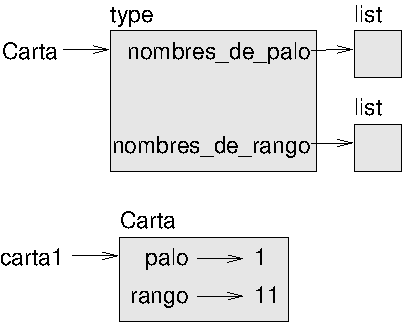
\includegraphics[scale=0.8]{figs/card1.pdf}}
\caption{Object diagram.}
\label{fig.card1}
\end{figure}

Figure~\ref{fig.card1} is a diagram of the {\tt Card} class object and
one Card instance.  {\tt Card} is a class object; its type is {\tt
  type}.  {\tt card1} is an instance of {\tt Card}, so its type is
{\tt Card}.  To save space, I didn't draw the contents of
\verb"suit_names" and \verb"rank_names".  \index{state diagram}
\index{diagram!state} \index{object diagram} \index{diagram!object}


\section{Comparing cards}
\label{comparecard}
\index{operator!relational}
\index{relational operator}

For built-in types, there are relational operators
({\tt <}, {\tt >}, {\tt ==}, etc.)
that compare
values and determine when one is greater than, less than, or equal to
another.  For programmer-defined types, we can override the behavior of
the built-in operators by providing a method named
\verb"__lt__", which stands for ``less than''.
\index{programmer-defined type}
\index{type!programmer-defined}

\verb"__lt__" takes two parameters, {\tt self} and {\tt other},
and returns {\tt True} if {\tt self} is strictly less than {\tt other}.
\index{override}
\index{operator overloading}

The correct ordering for cards is not obvious.
For example, which
is better, the 3 of Clubs or the 2 of Diamonds?  One has a higher
rank, but the other has a higher suit.  In order to compare
cards, you have to decide whether rank or suit is more important.

The answer might depend on what game you are playing, but to keep
things simple, we'll make the arbitrary choice that suit is more
important, so all of the Spades outrank all of the Diamonds,
and so on.
\index{cmp method@\_\_cmp\_\_ method}
\index{method!\_\_cmp\_\_}

With that decided, we can write \verb"__lt__":

\begin{verbatim}
# inside class Card:

    def __lt__(self, other):
        # check the suits
        if self.suit < other.suit: return True
        if self.suit > other.suit: return False

        # suits are the same... check ranks
        return self.rank < other.rank
\end{verbatim}
%
You can write this more concisely using tuple comparison:
\index{tuple!comparison}
\index{comparison!tuple}

\begin{verbatim}
# inside class Card:

    def __lt__(self, other):
        t1 = self.suit, self.rank
        t2 = other.suit, other.rank
        return t1 < t2
\end{verbatim}
%
As an exercise, write an \verb"__lt__" method for Time objects.  You
can use tuple comparison, but you also might consider
comparing integers.


\section{Decks}
\index{list!of objects}
\index{deck, playing cards}

Now that we have Cards, the next step is to define Decks.  Since a
deck is made up of cards, it is natural for each Deck to contain a
list of cards as an attribute.
\index{init method}
\index{method!init}

The following is a class definition for {\tt Deck}.  The
init method creates the attribute {\tt cards} and generates
the standard set of fifty-two cards:
\index{composition}
\index{loop!nested}
\index{Deck class}
\index{class!Deck}

\begin{verbatim}
class Deck:

    def __init__(self):
        self.cards = []
        for suit in range(4):
            for rank in range(1, 14):
                card = Card(suit, rank)
                self.cards.append(card)
\end{verbatim}
%
The easiest way to populate the deck is with a nested loop.  The outer
loop enumerates the suits from 0 to 3.  The inner loop enumerates the
ranks from 1 to 13.  Each iteration
creates a new Card with the current suit and rank,
and appends it to {\tt self.cards}.
\index{append method}
\index{method!append}


\section{Printing the deck}
\label{printdeck}
\index{str method@\_\_str\_\_ method}
\index{method!\_\_str\_\_}

Here is a \verb"__str__" method for {\tt Deck}:

\begin{verbatim}
#inside class Deck:

    def __str__(self):
        res = []
        for card in self.cards:
            res.append(str(card))
        return '\n'.join(res)
\end{verbatim}
%
This method demonstrates an efficient way to accumulate a large
string: building a list of strings and then using the string method
{\tt join}.  The built-in function {\tt str} invokes the
\verb"__str__" method on each card and returns the string
representation.  \index{accumulator!string} \index{string!accumulator}
\index{join method} \index{method!join} \index{newline}

Since we invoke {\tt join} on a newline character, the cards
are separated by newlines.  Here's what the result looks like:

\begin{verbatim}
>>> deck = Deck()
>>> print(deck)
Ace of Clubs
2 of Clubs
3 of Clubs
...
10 of Spades
Jack of Spades
Queen of Spades
King of Spades
\end{verbatim}
%
Even though the result appears on 52 lines, it is
one long string that contains newlines.


\section{Add, remove, shuffle and sort}

To deal cards, we would like a method that
removes a card from the deck and returns it.
The list method {\tt pop} provides a convenient way to do that:
\index{pop method}
\index{method!pop}

\begin{verbatim}
#inside class Deck:

    def pop_card(self):
        return self.cards.pop()
\end{verbatim}
%
Since {\tt pop} removes the {\em last} card in the list, we are
dealing from the bottom of the deck.
\index{append method}
\index{method!append}

To add a card, we can use the list method {\tt append}:

\begin{verbatim}
#inside class Deck:

    def add_card(self, card):
        self.cards.append(card)
\end{verbatim}
%
A method like this that uses another method without doing
much work is sometimes called a {\bf veneer}.  The metaphor
comes from woodworking, where a veneer is a thin
layer of good quality wood glued to the surface of a cheaper piece of
wood to improve the appearance.
\index{veneer}

In this case \verb"add_card" is a ``thin'' method that expresses
a list operation in terms appropriate for decks.  It
improves the appearance, or interface, of the
implementation.

As another example, we can write a Deck method named {\tt shuffle}
using the function {\tt shuffle} from the {\tt random} module:
\index{random module}
\index{module!random}
\index{shuffle function}
\index{function!shuffle}

\begin{verbatim}
# inside class Deck:

    def shuffle(self):
        random.shuffle(self.cards)
\end{verbatim}
%
Don't forget to import {\tt random}.

As an exercise, write a Deck method named {\tt sort} that uses the
list method {\tt sort} to sort the cards in a {\tt Deck}.  {\tt sort}
uses the \verb"__lt__" method we defined to determine the order.
\index{sort method} \index{method!sort}



\section{Inheritance}
\index{inheritance}
\index{object-oriented programming}

Inheritance is the ability to define a new class that is a modified
version of an existing class.  As an example, let's say we want a
class to represent a ``hand'', that is, the cards held by one player.
A hand is similar to a deck: both are made up of a collection of
cards, and both require operations like adding and removing cards.

A hand is also different from a deck; there are operations we want for
hands that don't make sense for a deck.  For example, in poker we
might compare two hands to see which one wins.  In bridge, we might
compute a score for a hand in order to make a bid.

This relationship between classes---similar, but different---lends
itself to inheritance.
To define a new class that inherits from an existing class,
you put the name of the existing class in parentheses:
\index{parentheses!parent class in}
\index{parent class}
\index{class!parent}
\index{Hand class}
\index{class!Hand}

\begin{verbatim}
class Hand(Deck):
    """Represents a hand of playing cards."""
\end{verbatim}
%
This definition indicates that {\tt Hand} inherits from {\tt Deck};
that means we can use methods like \verb"pop_card" and \verb"add_card"
for Hands as well as Decks.

When a new class inherits from an existing one, the existing
one is called the {\bf parent} and the new class is
called the {\bf child}.
\index{parent class}
\index{child class}
\index{class!child}

In this example, {\tt Hand} inherits \verb"__init__" from {\tt Deck},
but it doesn't really do what we want: instead of populating the hand
with 52 new cards, the init method for Hands should initialize {\tt
  cards} with an empty list.  \index{override} \index{init method}
\index{method!init}

If we provide an init method in the {\tt Hand} class, it overrides the
one in the {\tt Deck} class:

\begin{verbatim}
# inside class Hand:

    def __init__(self, label=''):
        self.cards = []
        self.label = label
\end{verbatim}
%
When you create a Hand, Python invokes this init method, not the
one in {\tt Deck}.

\begin{verbatim}
>>> hand = Hand('new hand')
>>> hand.cards
[]
>>> hand.label
'new hand'
\end{verbatim}
%
The other methods are inherited from {\tt Deck}, so we can use
\verb"pop_card" and \verb"add_card" to deal a card:

\begin{verbatim}
>>> deck = Deck()
>>> card = deck.pop_card()
>>> hand.add_card(card)
>>> print(hand)
King of Spades
\end{verbatim}
%
A natural next step is to encapsulate this code in a method
called \verb"move_cards":
\index{encapsulation}

\begin{verbatim}
#inside class Deck:

    def move_cards(self, hand, num):
        for i in range(num):
            hand.add_card(self.pop_card())
\end{verbatim}
%
\verb"move_cards" takes two arguments, a Hand object and the number of
cards to deal.  It modifies both {\tt self} and {\tt hand}, and
returns {\tt None}.

In some games, cards are moved from one hand to another,
or from a hand back to the deck.  You can use \verb"move_cards"
for any of these operations: {\tt self} can be either a Deck
or a Hand, and {\tt hand}, despite the name, can also be a {\tt Deck}.

Inheritance is a useful feature.  Some programs that would be
repetitive without inheritance can be written more elegantly
with it.  Inheritance can facilitate code reuse, since you can
customize the behavior of parent classes without having to modify
them.  In some cases, the inheritance structure reflects the natural
structure of the problem, which makes the design easier to
understand.

On the other hand, inheritance can make programs difficult to read.
When a method is invoked, it is sometimes not clear where to find its
definition.  The relevant code may be spread across several modules.
Also, many of the things that can be done using inheritance can be
done as well or better without it.


\section{Class diagrams}
\label{class.diagram}

So far we have seen stack diagrams, which show the state of
a program, and object diagrams, which show the attributes
of an object and their values.  These diagrams represent a snapshot
in the execution of a program, so they change as the program
runs.

They are also highly detailed; for some purposes, too
detailed.  A class diagram is a more abstract representation
of the structure of a program.  Instead of showing individual
objects, it shows classes and the relationships between them.

There are several kinds of relationship between classes:

\begin{itemize}

\item Objects in one class might contain references to objects
in another class.  For example, each Rectangle contains a reference
to a Point, and each Deck contains references to many Cards.
This kind of relationship is called {\bf HAS-A}, as in, ``a Rectangle
has a Point.''

\item One class might inherit from another.  This relationship
is called {\bf IS-A}, as in, ``a Hand is a kind of a Deck.''

\item One class might depend on another in the sense that objects
in one class take objects in the second class as parameters, or
use objects in the second class as part of a computation.  This
kind of relationship is called a {\bf dependency}.

\end{itemize}
\index{IS-A relationship}
\index{HAS-A relationship}
\index{class diagram}
\index{diagram!class}

A {\bf class diagram} is a graphical representation of these
relationships.  For example, Figure~\ref{fig.class1} shows the
relationships between {\tt Card}, {\tt Deck} and {\tt Hand}.

\begin{figure}
\centerline
{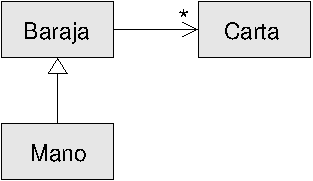
\includegraphics[scale=0.8]{figs/class1.pdf}}
\caption{Class diagram.}
\label{fig.class1}
\end{figure}

The arrow with a hollow triangle head represents an IS-A
relationship; in this case it indicates that Hand inherits
from Deck.

The standard arrow head represents a HAS-A
relationship; in this case a Deck has references to Card
objects.
\index{multiplicity (in class diagram)}

The star ({\tt *}) near the arrow head is a
{\bf multiplicity}; it indicates how many Cards a Deck has.
A multiplicity can be a simple number, like {\tt 52}, a range,
like {\tt 5..7} or a star, which indicates that a Deck can
have any number of Cards.

There are no dependencies in this diagram.  They would normally
be shown with a dashed arrow.  Or if there are a lot of
dependencies, they are sometimes omitted.

A more detailed diagram might show that a Deck actually
contains a {\em list} of Cards, but built-in types
like list and dict are usually not included in class diagrams.


\section{Debugging}
\index{debugging}

Inheritance can make debugging difficult because when you invoke a
method on an object, it might be hard to figure out which method will
be invoked.
\index{inheritance}

Suppose you are writing a function that works with Hand objects.
You would like it to work with all kinds of Hands, like
PokerHands, BridgeHands, etc.  If you invoke a method like
{\tt shuffle}, you might get the one defined in {\tt Deck},
but if any of the subclasses override this method, you'll
get that version instead.  This behavior is usually a good
thing, but it can be confusing.

Any time you are unsure about the flow of execution through your
program, the simplest solution is to add print statements at the
beginning of the relevant methods.  If {\tt Deck.shuffle} prints a
message that says something like {\tt Running Deck.shuffle}, then as
the program runs it traces the flow of execution.
\index{flow of execution}

As an alternative, you could use this function, which takes an
object and a method name (as a string) and returns the class that
provides the definition of the method:

\begin{verbatim}
def find_defining_class(obj, meth_name):
    for ty in type(obj).mro():
        if meth_name in ty.__dict__:
            return ty
\end{verbatim}
%
Here's an example:

\begin{verbatim}
>>> hand = Hand()
>>> find_defining_class(hand, 'shuffle')
<class '__main__.Deck'>
\end{verbatim}
%
So the {\tt shuffle} method for this Hand is the one in {\tt Deck}.
\index{mro method}
\index{method!mro}
\index{method resolution order}

\verb"find_defining_class" uses the {\tt mro} method to get the list
of class objects (types) that will be searched for methods.  ``MRO''
stands for ``method resolution order'', which is the sequence of
classes Python searches to ``resolve'' a method name.

Here's a design suggestion: when you override a method,
the interface of the new method should be the same as the old.  It
should take the same parameters, return the same type, and obey the
same preconditions and postconditions.  If you follow this rule, you
will find that any function designed to work with an instance of a
parent class, like a Deck, will also work with instances of child
classes like a Hand and PokerHand.
\index{override}
\index{interface}
\index{precondition}
\index{postcondition}

If you violate this rule, which is called the ``Liskov substitution
principle'', your code will collapse like (sorry) a house of cards.
\index{Liskov substitution principle}


\section{Data encapsulation}

The previous chapters demonstrate a development plan we might call
``object-oriented design''.  We identified objects we needed---like
{\tt Point}, {\tt Rectangle} and {\tt Time}---and defined classes to
represent them.  In each case there is an obvious correspondence
between the object and some entity in the real world (or at least a
mathematical world).
\index{development plan!data encapsulation}

But sometimes it is less obvious what objects you need
and how they should interact.  In that case you need a different
development plan.  In the same way that we discovered function
interfaces by encapsulation and generalization, we can discover
class interfaces by {\bf data encapsulation}.
\index{data encapsulation}

Markov analysis, from Section~\ref{markov}, provides a good example.
If you download my code from \url{http://thinkpython2.com/code/markov.py},
you'll see that it uses two global variables---\verb"suffix_map" and
\verb"prefix"---that are read and written from several functions.

\begin{verbatim}
suffix_map = {}
prefix = ()
\end{verbatim}

Because these variables are global, we can only run one analysis at a
time.  If we read two texts, their prefixes and suffixes would be
added to the same data structures (which makes for some interesting
generated text).

To run multiple analyses, and keep them separate, we can encapsulate
the state of each analysis in an object.
Here's what that looks like:

\begin{verbatim}
class Markov:

    def __init__(self):
        self.suffix_map = {}
        self.prefix = ()
\end{verbatim}

Next, we transform the functions into methods.  For example,
here's \verb"process_word":

\begin{verbatim}
    def process_word(self, word, order=2):
        if len(self.prefix) < order:
            self.prefix += (word,)
            return

        try:
            self.suffix_map[self.prefix].append(word)
        except KeyError:
            # if there is no entry for this prefix, make one
            self.suffix_map[self.prefix] = [word]

        self.prefix = shift(self.prefix, word)
\end{verbatim}

Transforming a program like this---changing the design without
changing the behavior---is another example of refactoring
(see Section~\ref{refactoring}).
\index{refactoring}

This example suggests a development plan for designing objects and
methods:

\begin{enumerate}

\item Start by writing functions that read and write global
variables (when necessary).

\item Once you get the program working, look for associations
between global variables and the functions that use them.

\item Encapsulate related variables as attributes of an object.

\item Transform the associated functions into methods of the new
class.

\end{enumerate}

As an exercise, download my Markov code from
\url{http://thinkpython2.com/code/markov.py}, and follow the steps
described above to encapsulate the global variables as attributes of a
new class called {\tt Markov}.  Solution:
\url{http://thinkpython2.com/code/markov2.py}.


\section{Glossary}

\begin{description}

\item[encode:]  To represent one set of values using another
set of values by constructing a mapping between them.
\index{encode}

\item[class attribute:] An attribute associated with a class
object.  Class attributes are defined inside
a class definition but outside any method.
\index{class attribute}
\index{attribute!class}

\item[instance attribute:] An attribute associated with an
instance of a class.
\index{instance attribute}
\index{attribute!instance}

\item[veneer:] A method or function that provides a different
interface to another function without doing much computation.
\index{veneer}

\item[inheritance:] The ability to define a new class that is a
modified version of a previously defined class.
\index{inheritance}

\item[parent class:] The class from which a child class inherits.
\index{parent class}

\item[child class:] A new class created by inheriting from an
existing class; also called a ``subclass''.
\index{child class}
\index{class!child}

\item[IS-A relationship:] A relationship between a child class
and its parent class.
\index{IS-A relationship}

\item[HAS-A relationship:] A relationship between two classes
where instances of one class contain references to instances of
the other.
\index{HAS-A relationship}

\item[dependency:] A relationship between two classes
where instances of one class use instances of the other class,
but do not store them as attributes.
\index{HAS-A relationship}

\item[class diagram:] A diagram that shows the classes in a program
and the relationships between them.
\index{class diagram}
\index{diagram!class}

\item[multiplicity:] A notation in a class diagram that shows, for
a HAS-A relationship, how many references there are to instances
of another class.
\index{multiplicity (in class diagram)}

\item[data encapsulation:]  A program development plan that
involves a prototype using global variables and a final version
that makes the global variables into instance attributes.
\index{data encapsulation}
\index{development plan!data encapsulation}

\end{description}


\section{Exercises}

\begin{exercise}
For the following program, draw a UML class diagram that shows
these classes and the relationships among them.

\begin{verbatim}
class PingPongParent:
    pass

class Ping(PingPongParent):
    def __init__(self, pong):
        self.pong = pong


class Pong(PingPongParent):
    def __init__(self, pings=None):
        if pings is None:
            self.pings = []
        else:
            self.pings = pings

    def add_ping(self, ping):
        self.pings.append(ping)

pong = Pong()
ping = Ping(pong)
pong.add_ping(ping)
\end{verbatim}


\end{exercise}



\begin{exercise}
Write a Deck method called \verb"deal_hands" that
takes two parameters, the number of hands and the number of cards per
hand.  It should create the appropriate number of Hand objects, deal
the appropriate number of cards per hand, and return a list of Hands.
\end{exercise}


\begin{exercise}
\label{poker}

The following are the possible hands in poker, in increasing order
of value and decreasing order of probability:
\index{poker}

\begin{description}

\item[pair:] two cards with the same rank
\vspace{-0.05in}

\item[two pair:] two pairs of cards with the same rank
\vspace{-0.05in}

\item[three of a kind:] three cards with the same rank
\vspace{-0.05in}

\item[straight:] five cards with ranks in sequence (aces can
be high or low, so {\tt Ace-2-3-4-5} is a straight and so is {\tt
10-Jack-Queen-King-Ace}, but {\tt Queen-King-Ace-2-3} is not.)
\vspace{-0.05in}

\item[flush:] five cards with the same suit
\vspace{-0.05in}

\item[full house:] three cards with one rank, two cards with another
\vspace{-0.05in}

\item[four of a kind:] four cards with the same rank
\vspace{-0.05in}

\item[straight flush:] five cards in sequence (as defined above) and
with the same suit
\vspace{-0.05in}

\end{description}
%
The goal of these exercises is to estimate
the probability of drawing these various hands.

\begin{enumerate}

\item Download the following files from \url{http://thinkpython2.com/code}:

\begin{description}

\item[{\tt Card.py}]: A complete version of the {\tt Card},
{\tt Deck} and {\tt Hand} classes in this chapter.

\item[{\tt PokerHand.py}]: An incomplete implementation of a class
that represents a poker hand, and some code that tests it.

\end{description}
%
\item If you run {\tt PokerHand.py}, it deals seven 7-card poker hands
and checks to see if any of them contains a flush.  Read this
code carefully before you go on.

\item Add methods to {\tt PokerHand.py} named \verb"has_pair",
\verb"has_twopair", etc. that return True or False according to
whether or not the hand meets the relevant criteria.  Your code should
work correctly for ``hands'' that contain any number of cards
(although 5 and 7 are the most common sizes).

\item Write a method named {\tt classify} that figures out
the highest-value classification for a hand and sets the
{\tt label} attribute accordingly.  For example, a 7-card hand
might contain a flush and a pair; it should be labeled ``flush''.

\item When you are convinced that your classification methods are
working, the next step is to estimate the probabilities of the various
hands.  Write a function in {\tt PokerHand.py} that shuffles a deck of
cards, divides it into hands, classifies the hands, and counts the
number of times various classifications appear.

\item Print a table of the classifications and their probabilities.
Run your program with larger and larger numbers of hands until the
output values converge to a reasonable degree of accuracy.  Compare
your results to the values at \url{http://en.wikipedia.org/wiki/Hand_rankings}.

\end{enumerate}

Solution: \url{http://thinkpython2.com/code/PokerHandSoln.py}.
\end{exercise}


\chapter{The Goodies}

One of my goals for this book has been to teach you as little Python
as possible.  When there were two ways to do something, I picked
one and avoided mentioning the other.  Or sometimes I put the second
one into an exercise.

Now I want to go back for some of the good bits that got left behind.
Python provides a number of features that are not really necessary---you
can write good code without them---but with them you can sometimes
write code that's more concise, readable or efficient, and sometimes
all three.

% TODO: add the with statement

\section{Conditional expressions}

We saw conditional statements in Section~\ref{conditional.execution}.
Conditional statements are often used to choose one of two values;
for example:
\index{conditional expression}
\index{expression!conditional}

\begin{verbatim}
if x > 0:
    y = math.log(x)
else:
    y = float('nan')
\end{verbatim}

This statement checks whether {\tt x} is positive.  If so, it computes
{\tt math.log}.  If not, {\tt math.log} would raise a ValueError.  To
avoid stopping the program, we generate a ``NaN'', which is a special
floating-point value that represents ``Not a Number''.
\index{NaN}
\index{floating-point}

We can write this statement more concisely using a {\bf conditional
expression}:

\begin{verbatim}
y = math.log(x) if x > 0 else float('nan')
\end{verbatim}

You can almost read this line like English: ``{\tt y} gets log-{\tt x}
if {\tt x} is greater than 0; otherwise it gets NaN''.

Recursive functions can sometimes be rewritten using conditional
expressions.  For example, here is a recursive version of {\tt factorial}:
\index{factorial}
\index{function!factorial}

\begin{verbatim}
def factorial(n):
    if n == 0:
        return 1
    else:
        return n * factorial(n-1)
\end{verbatim}

We can rewrite it like this:

\begin{verbatim}
def factorial(n):
    return 1 if n == 0 else n * factorial(n-1)
\end{verbatim}

Another use of conditional expressions is handling optional
arguments.  For example, here is the init method from
{\tt GoodKangaroo} (see Exercise~\ref{kangaroo}):
\index{optional argument}
\index{argument!optional}

\begin{verbatim}
    def __init__(self, name, contents=None):
        self.name = name
        if contents == None:
            contents = []
        self.pouch_contents = contents
\end{verbatim}

We can rewrite this one like this:

\begin{verbatim}
    def __init__(self, name, contents=None):
        self.name = name
        self.pouch_contents = [] if contents == None else contents
\end{verbatim}

In general, you can replace a conditional statement with a conditional
expression if both branches contain simple expressions that are
either returned or assigned to the same variable.
\index{conditional statement}
\index{statement!conditional}



\section{List comprehensions}

In Section~\ref{filter} we saw the map and filter patterns.  For
example, this function takes a list of strings, maps the string method
{\tt capitalize} to the elements, and returns a new list of strings:

\begin{verbatim}
def capitalize_all(t):
    res = []
    for s in t:
        res.append(s.capitalize())
    return res
\end{verbatim}

We can write this more concisely using a {\bf list comprehension}:
\index{list comprehension}

\begin{verbatim}
def capitalize_all(t):
    return [s.capitalize() for s in t]
\end{verbatim}

The bracket operators indicate that we are constructing a new
list.  The expression inside the brackets specifies the elements
of the list, and the {\tt for} clause indicates what sequence
we are traversing.
\index{list}
\index{for loop}

The syntax of a list comprehension is a little awkward because
the loop variable, {\tt s} in this example, appears in the expression
before we get to the definition.
\index{loop variable}

List comprehensions can also be used for filtering.  For example,
this function selects only the elements of {\tt t} that are
upper case, and returns a new list:
\index{filter pattern}
\index{pattern!filter}

\begin{verbatim}
def only_upper(t):
    res = []
    for s in t:
        if s.isupper():
            res.append(s)
    return res
\end{verbatim}

We can rewrite it using a list comprehension

\begin{verbatim}
def only_upper(t):
    return [s for s in t if s.isupper()]
\end{verbatim}

List comprehensions are concise and easy to read, at least for simple
expressions.  And they are usually faster than the equivalent for
loops, sometimes much faster.  So if you are mad at me for not
mentioning them earlier, I understand.

But, in my defense, list comprehensions are harder to debug because
you can't put a print statement inside the loop.  I suggest that you
use them only if the computation is simple enough that you are likely
to get it right the first time.  And for beginners that means never.
\index{debugging}



\section{Generator expressions}

{\bf Generator expressions} are similar to list comprehensions, but
with parentheses instead of square brackets:
\index{generator expression}
\index{expression!generator}

\begin{verbatim}
>>> g = (x**2 for x in range(5))
>>> g
<generator object <genexpr> at 0x7f4c45a786c0>
\end{verbatim}
%
The result is a generator object that knows how to iterate through
a sequence of values.  But unlike a list comprehension, it does not
compute the values all at once; it waits to be asked.  The built-in
function {\tt next} gets the next value from the generator:
\index{generator object}
\index{object!generator}

\begin{verbatim}
>>> next(g)
0
>>> next(g)
1
\end{verbatim}
%
When you get to the end of the sequence, {\tt next} raises a
StopIteration exception.  You can also use a {\tt for} loop to iterate
through the values:
\index{StopIteration}
\index{exception!StopIteration}

\begin{verbatim}
>>> for val in g:
...     print(val)
4
9
16
\end{verbatim}
%
The generator object keeps track of where it is in the sequence,
so the {\tt for} loop picks up where {\tt next} left off.  Once the
generator is exhausted, it continues to raise {\tt StopIteration}:

\begin{verbatim}
>>> next(g)
StopIteration
\end{verbatim}

Generator expressions are often used with functions like {\tt sum},
{\tt max}, and {\tt min}:
\index{sum}
\index{function!sum}

\begin{verbatim}
>>> sum(x**2 for x in range(5))
30
\end{verbatim}


\section{{\tt any} and {\tt all}}

Python provides a built-in function, {\tt any}, that takes a sequence
of boolean values and returns {\tt True} if any of the values are {\tt
  True}.  It works on lists:
\index{any}
\index{built-in function!any}

\begin{verbatim}
>>> any([False, False, True])
True
\end{verbatim}
%
But it is often used with generator expressions:
\index{generator expression}
\index{expression!generator}

\begin{verbatim}
>>> any(letter == 't' for letter in 'monty')
True
\end{verbatim}
%
That example isn't very useful because it does the same thing
as the {\tt in} operator.  But we could use {\tt any} to rewrite
some of the search functions we wrote in Section~\ref{search}.  For
example, we could write {\tt avoids} like this:
\index{search pattern}
\index{pattern!search}

\begin{verbatim}
def avoids(word, forbidden):
    return not any(letter in forbidden for letter in word)
\end{verbatim}
%
The function almost reads like English, ``{\tt word} avoids
{\tt forbidden} if there are not any forbidden letters in {\tt word}.''

Using {\tt any} with a generator expression is efficient because
it stops immediately if it finds a {\tt True} value,
so it doesn't have to evaluate the whole sequence.

Python provides another built-in function, {\tt all}, that returns
{\tt True} if every element of the sequence is {\tt True}.  As
an exercise, use {\tt all} to re-write \verb"uses_all" from
Section~\ref{search}.
\index{all}
\index{built-in function!any}


\section{Sets}
\label{sets}

In Section~\ref{dictsub} I use dictionaries to find the words
that appear in a document but not in a word list.  The function
I wrote takes {\tt d1}, which contains the words from the document
as keys, and {\tt d2}, which contains the list of words.  It
returns a dictionary that contains the keys from {\tt d1} that
are not in {\tt d2}.

\begin{verbatim}
def subtract(d1, d2):
    res = dict()
    for key in d1:
        if key not in d2:
            res[key] = None
    return res
\end{verbatim}
%
In all of these dictionaries, the values are {\tt None} because
we never use them.  As a result, we waste some storage space.
\index{dictionary subtraction}

Python provides another built-in type, called a {\tt set}, that
behaves like a collection of dictionary keys with no values.  Adding
elements to a set is fast; so is checking membership.  And sets
provide methods and operators to compute common set operations.
\index{set}
\index{object!set}

For example, set subtraction is available as a method called
{\tt difference} or as an operator, {\tt -}.  So we can rewrite
{\tt subtract} like this:
\index{set subtraction}

\begin{verbatim}
def subtract(d1, d2):
    return set(d1) - set(d2)
\end{verbatim}
%
The result is a set instead of a dictionary, but for operations like
iteration, the behavior is the same.

Some of the exercises in this book can be done concisely and
efficiently with sets.  For example, here is a solution to
\verb"has_duplicates", from
Exercise~\ref{duplicate}, that uses a dictionary:

\begin{verbatim}
def has_duplicates(t):
    d = {}
    for x in t:
        if x in d:
            return True
        d[x] = True
    return False
\end{verbatim}

When an element appears for the first time, it is added to the
dictionary.  If the same element appears again, the function returns
{\tt True}.

Using sets, we can write the same function like this:

\begin{verbatim}
def has_duplicates(t):
    return len(set(t)) < len(t)
\end{verbatim}
%
An element can only appear in a set once, so if an element in {\tt t}
appears more than once, the set will be smaller than {\tt t}.  If there
are no duplicates, the set will be the same size as {\tt t}.
\index{duplicate}

We can also use sets to do some of the exercises in
Chapter~\ref{wordplay}.  For example, here's a version of
\verb"uses_only" with a loop:

\begin{verbatim}
def uses_only(word, available):
    for letter in word:
        if letter not in available:
            return False
    return True
\end{verbatim}
%
\verb"uses_only" checks whether all letters in {\tt word} are
in {\tt available}.  We can rewrite it like this:

\begin{verbatim}
def uses_only(word, available):
    return set(word) <= set(available)
\end{verbatim}
%
The \verb"<=" operator checks whether one set is a subset of another,
including the possibility that they are equal, which is true if all
the letters in {\tt word} appear in {\tt available}.
\index{subset}

As an exercise, rewrite \verb"avoids" using sets.


\section{Counters}

A Counter is like a set, except that if an element appears more
than once, the Counter keeps track of how many times it appears.
If you are familiar with the mathematical idea of a {\bf multiset},
a Counter is a natural way to represent a multiset.
\index{Counter}
\index{object!Counter}
\index{multiset}

Counter is defined in a standard module called {\tt collections},
so you have to import it.  You can initialize a Counter with a string,
list, or anything else that supports iteration:
\index{collections}
\index{module!collections}

\begin{verbatim}
>>> from collections import Counter
>>> count = Counter('parrot')
>>> count
Counter({'r': 2, 't': 1, 'o': 1, 'p': 1, 'a': 1})
\end{verbatim}

Counters behave like dictionaries in many ways; they map from each
key to the number of times it appears.  As in dictionaries,
the keys have to be hashable.

Unlike dictionaries, Counters don't raise an exception if you access
an element that doesn't appear.  Instead, they return 0:

\begin{verbatim}
>>> count['d']
0
\end{verbatim}

We can use Counters to rewrite \verb"is_anagram" from
Exercise~\ref{anagram}:

\begin{verbatim}
def is_anagram(word1, word2):
    return Counter(word1) == Counter(word2)
\end{verbatim}

If two words are anagrams, they contain the same letters with the same
counts, so their Counters are equivalent.

Counters provide methods and operators to perform set-like operations,
including addition, subtraction, union and intersection.  And
they provide an often-useful method, \verb"most_common", which
returns a list of value-frequency pairs, sorted from most common to
least:

\begin{verbatim}
>>> count = Counter('parrot')
>>> for val, freq in count.most_common(3):
...     print(val, freq)
r 2
p 1
a 1
\end{verbatim}


\section{defaultdict}

The {\tt collections} module also provides {\tt defaultdict}, which is
like a dictionary except that if you access a key that doesn't exist,
it can generate a new value on the fly.
\index{defaultdict}
\index{object!defaultdict}
\index{collections}
\index{module!collections}

When you create a defaultdict, you provide a function that's used to
create new values.  A function used to create objects is sometimes
called a {\bf factory}.  The built-in functions that create lists, sets,
and other types can be used as factories:
\index{factory function}

\begin{verbatim}
>>> from collections import defaultdict
>>> d = defaultdict(list)
\end{verbatim}

Notice that the argument is {\tt list}, which is a class object,
not {\tt list()}, which is a new list.  The function you provide
doesn't get called unless you access a key that doesn't exist.

\begin{verbatim}
>>> t = d['new key']
>>> t
[]
\end{verbatim}

The new list, which we're calling {\tt t}, is also added to the
dictionary.  So if we modify {\tt t}, the change appears in {\tt d}:

\begin{verbatim}
>>> t.append('new value')
>>> d
defaultdict(<class 'list'>, {'new key': ['new value']})
\end{verbatim}

If you are making a dictionary of lists, you can often write simpler
code using {\tt defaultdict}.  In my solution to
Exercise~\ref{anagrams}, which you can get from
\url{http://thinkpython2.com/code/anagram_sets.py}, I make a
dictionary that maps from a sorted string of letters to the list of
words that can be spelled with those letters.  For example, {\tt
  'opst'} maps to the list {\tt ['opts', 'post', 'pots', 'spot',
    'stop', 'tops']}.

Here's the original code:

\begin{verbatim}
def all_anagrams(filename):
    d = {}
    for line in open(filename):
        word = line.strip().lower()
        t = signature(word)
        if t not in d:
            d[t] = [word]
        else:
            d[t].append(word)
    return d
\end{verbatim}

This can be simplified using {\tt setdefault}, which you might
have used in Exercise~\ref{setdefault}:
\index{setdefault}

\begin{verbatim}
def all_anagrams(filename):
    d = {}
    for line in open(filename):
        word = line.strip().lower()
        t = signature(word)
        d.setdefault(t, []).append(word)
    return d
\end{verbatim}

This solution has the drawback that it makes a new list
every time, regardless of whether it is needed.  For lists,
that's no big deal, but if the factory
function is complicated, it might be.
\index{factory function}

We can avoid this problem and
simplify the code using a {\tt defaultdict}:

\begin{verbatim}
def all_anagrams(filename):
    d = defaultdict(list)
    for line in open(filename):
        word = line.strip().lower()
        t = signature(word)
        d[t].append(word)
    return d
\end{verbatim}

My solution to Exercise~\ref{poker}, which you can download from
\url{http://thinkpython2.com/code/PokerHandSoln.py},
uses {\tt setdefault} in the function
\verb"has_straightflush".  This solution has the drawback
of creating a {\tt Hand} object every time through the loop, whether
it is needed or not.  As an exercise, rewrite it using
a defaultdict.


\section{Named tuples}

Many simple objects are basically collections of related values.
For example, the Point object defined in Chapter~\ref{clobjects} contains
two numbers, {\tt x} and {\tt y}.  When you define a class like
this, you usually start with an init method and a str method:

\begin{verbatim}
class Point:

    def __init__(self, x=0, y=0):
        self.x = x
        self.y = y

    def __str__(self):
        return '(%g, %g)' % (self.x, self.y)
\end{verbatim}

This is a lot of code to convey a small amount of information.
Python provides a more concise way to say the same thing:

\begin{verbatim}
from collections import namedtuple
Point = namedtuple('Point', ['x', 'y'])
\end{verbatim}

The first argument is the name of the class you want to create.
The second is a list of the attributes Point objects should have,
as strings.  The return value from {\tt namedtuple} is a class object:
\index{namedtuple}
\index{object!namedtuple}
\index{collections}
\index{module!collections}

\begin{verbatim}
>>> Point
<class '__main__.Point'>
\end{verbatim}

{\tt Point} automatically provides methods like \verb"__init__" and
\verb"__str__" so you don't have to write them.
\index{class object}
\index{object!class}

To create a Point object, you use the Point class as a function:

\begin{verbatim}
>>> p = Point(1, 2)
>>> p
Point(x=1, y=2)
\end{verbatim}

The init method assigns the arguments to attributes using the names
you provided.  The str method prints a representation of the Point
object and its attributes.

You can access the elements of the named tuple by name:

\begin{verbatim}
>>> p.x, p.y
(1, 2)
\end{verbatim}

But you can also treat a named tuple as a tuple:

\begin{verbatim}
>>> p[0], p[1]
(1, 2)

>>> x, y = p
>>> x, y
(1, 2)
\end{verbatim}

Named tuples provide a quick way to define simple classes.
The drawback is that simple classes don't always stay simple.
You might decide later that you want to add methods to a named tuple.
In that case, you could define a new class that inherits from
the named tuple:
\index{inheritance}

\begin{verbatim}
class Pointier(Point):
    # add more methods here
\end{verbatim}

Or you could switch to a conventional class definition.


\section{Gathering keyword args}

In Section~\ref{gather}, we saw how to write a function that
gathers its arguments into a tuple:
\index{gather}

\begin{verbatim}
def printall(*args):
    print(args)
\end{verbatim}
%
You can call this function with any number of positional arguments
(that is, arguments that don't have keywords):
\index{positional argument}
\index{argument!positional}

\begin{verbatim}
>>> printall(1, 2.0, '3')
(1, 2.0, '3')
\end{verbatim}
%
But the {\tt *} operator doesn't gather keyword arguments:
\index{keyword argument}
\index{argument!keyword}

\begin{verbatim}
>>> printall(1, 2.0, third='3')
TypeError: printall() got an unexpected keyword argument 'third'
\end{verbatim}
%
To gather keyword arguments, you can use the {\tt **} operator:

\begin{verbatim}
def printall(*args, **kwargs):
    print(args, kwargs)
\end{verbatim}
%
You can call the keyword gathering parameter anything you want, but
{\tt kwargs} is a common choice.  The result is a dictionary that maps
keywords to values:

\begin{verbatim}
>>> printall(1, 2.0, third='3')
(1, 2.0) {'third': '3'}
\end{verbatim}
%
If you have a dictionary of keywords and values, you can use the
scatter operator, {\tt **} to call a function:
\index{scatter}

\begin{verbatim}
>>> d = dict(x=1, y=2)
>>> Point(**d)
Point(x=1, y=2)
\end{verbatim}
%
Without the scatter operator, the function would treat {\tt d} as
a single positional argument, so it would assign {\tt d} to
{\tt x} and complain because there's nothing to assign to {\tt y}:

\begin{verbatim}
>>> d = dict(x=1, y=2)
>>> Point(d)
Traceback (most recent call last):
  File "<stdin>", line 1, in <module>
TypeError: __new__() missing 1 required positional argument: 'y'
\end{verbatim}
%
When you are working with functions that have a large number of
parameters, it is often useful to create and pass around dictionaries
that specify frequently used options.


\section{Glossary}

\begin{description}

\item[conditional expression:] An expression that has one of two
values, depending on a condition.
\index{conditional expression}
\index{expression!conditional}

\item[list comprehension:] An expression with a {\tt for} loop in square
brackets that yields a new list.
\index{list comprehension}

\item[generator expression:] An expression with a {\tt for} loop in parentheses
that yields a generator object.
\index{generator expression}
\index{expression!generator}

\item[multiset:] A mathematical entity that represents a mapping
between the elements of a set and the number of times they appear.

\item[factory:] A function, usually passed as a parameter, used to
create objects.
\index{factory}

\end{description}




\section{Exercises}

\begin{exercise}

The following is a function computes the binomial
coefficient recursively.

\begin{verbatim}
def binomial_coeff(n, k):
    """Compute the binomial coefficient "n choose k".

    n: number of trials
    k: number of successes

    returns: int
    """
    if k == 0:
        return 1
    if n == 0:
        return 0

    res = binomial_coeff(n-1, k) + binomial_coeff(n-1, k-1)
    return res
\end{verbatim}

Rewrite the body of the function using nested conditional
expressions.

One note: this function is not very efficient because it ends up computing
the same values over and over.  You could make it more efficient by
memoizing (see Section~\ref{memoize}).  But you will find that it's harder to
memoize if you write it using conditional expressions.

\end{exercise}



\appendix

\chapter{Depuración}
\index{debugging}

Cuando estés depurando, deberías distinguir entre los diferentes
tipos de errores con el fin de rastrearlos de manera más rápida:

\begin{itemize}

\item Los errores de sintaxis son descubiertos por el intérprete cuando está
  traduciendo el código fuente a código byte.  Indican
  que hay algo mal en la estructura del programa.
  Ejemplo: omitir el signo de dos puntos al final de una sentencia {\tt def}
  genera el mensaje algo redundante {\tt SyntaxError: invalid
    syntax}.
\index{error de sintaxis}
\index{sintaxis!error de}

\item Los errores de tiempo de ejecución son producidos por el intérprete si algo va
  mal mientras el programa se está ejecutando.  La mayoría de los mensajes de error de tiempo de ejecución
  incluyen información acerca de dónde ocurrió el error y qué
  funciones se estaban ejecutando.  Ejemplo: una recursividad infinita eventualmente
  causa el error de tiempo de ejecución ``maximum recursion depth exceeded''.
\index{error de tiempo de ejecución}
\index{tiempo de ejecución!error de}
\index{excepción}

\item Los errores semánticos son problemas que tiene un programa que se ejecuta sin
  producir mensajes de error pero sin hacer lo correcto.  Ejemplo:
  una expresión puede que no sea evaluada en el orden que esperas, entregando
  un resultado incorrecto.
\index{error semántico}
\index{semántico!error}

\end{itemize}

El primer paso en la depuración es averiguar con qué tipo de
error estás lidiando.  Aunque las siguientes secciones están
organizadas por tipo de error, algunas técnicas son
aplicables en más de una situación.


\section{Errores de sintaxis}
\index{mensaje de error}

Los errores de sintaxis son generalmente fáciles de arreglar una vez que averiguas cuáles
son.  Desafortunadamente, los mensajes de error a menudo no son útiles.
Los mensajes más comunes son {\tt SyntaxError: invalid syntax} y
{\tt SyntaxError: invalid token}, de los cuales ninguno es muy informativo.

Por otra parte, el mensaje sí te dice el lugar del programa donde
ocurrió el problema.  En realidad, te dice dónde Python
notó un problema, que no necesariamente es donde está
el error.  A veces el error está antes de la ubicación del mensaje
de error, a menudo en la línea precedente.
\index{desarrollo incremental}
\index{plan de desarrollo!incremental}

Si estás construyendo el programa de manera incremental, deberías tener
una buena idea acerca de dónde está el error.  Estará en la última
línea que agregaste.

Si estás copiando código de un libro, comienza comparando
tu código con el código del libro muy cuidadosamente.  Revisa cada carácter.
Al mismo tiempo, recuerda que el libro podría estar mal, por tanto
si ves algo que parece un error de sintaxis, puede serlo.

Aquí hay algunas maneras de evitar los errores de sintaxis más comunes:
\index{sintaxis}

\begin{enumerate}

\item Asegúrate de que no estás usando una palabra clave de Python para un nombre de variable.
\index{palabra clave}

\item Verifica que tienes un signo de dos puntos al final del encabezado de cada
sentencia compuesta, incluyendo las sentencias {\tt for}, {\tt while},
{\tt if} y {\tt def}.
\index{encabezado}
\index{signo de dos puntos}

\item Asegúrate de que todas las cadenas en el código tengan comillas
coincidentes.  Asegúrate de que todas las comillas son
``comillas rectas'', no ``comillas tipográficas''.
\index{comillas}

\item Si tienes cadenas multilínea con comillas triples (simples o dobles),
asegúrate de que has terminado la cadena de manera apropiada.  Una cadena sin terminar
puede causar un error {\tt invalid token} al final de tu programa,
o puede tratar la siguiente parte del programa como una cadena hasta que
llega a la siguiente cadena.  En el segundo caso, ¡podría no producir ningún mensaje
de error!
\index{cadena multilínea}
\index{multilínea!cadena}

\item Un operador de apertura no cerrado ---\verb+(+, \verb+{+ o
  \verb+[+--- hace que Python continúe con la línea siguiente como parte de la
  sentencia actual.  Generalmente, ocurre un error casi inmediatamente en
  la línea siguiente.

\item Revisa el clásico {\tt =} en lugar de {\tt ==} dentro
de un condicional.
\index{condicional}

\item Revisa la sangría para asegurarte de que esté alineada como se
supone que debe.  Python puede manejar el espacio y la tabulación, pero si los mezclas
puede causar problemas.  La mejor manera de evitar este problema
es usar un editor de texto que sepa sobre Python y genere
sangría consistente.
\index{sangría}
\index{espacio en blanco}

\item Si tienes caracteres no ASCII en el código (incluyendo cadenas
y comentarios), podría causar un problema, aunque Python 3 generalmente
maneja caracteres no ASCII.  Ten cuidado si pegas texto de
una página web u otra fuente.

\end{enumerate}

Si nada funciona, pasa a la siguiente sección...


\subsection{Sigo haciendo cambios y no hay diferencia.}

Si el intérprete dice que hay un error y tú no lo ves,
podría ser porque tú y el intérprete no están mirando el mismo
código.  Revisa tu entorno de programación para asegurarte de que el
programa que estás editando es el que Python está intentando ejecutar.

Si no estás seguro, intenta poniendo un error de sintaxis obvio y deliberado
al principio del programa.  Ahora ejecútalo de nuevo.  Si el
intérprete no encuentra el nuevo error, no estás ejecutando el
código nuevo.

Hay algunos posibles culpables:

\begin{itemize}

\item Editaste el archivo y olvidaste guardar los cambios antes de
ejecutarlo de nuevo.  Algunos entornos de programación hacen esto
por ti, pero otros no.

\item Cambiaste el nombre del archivo, pero todavía estás ejecutando
el nombre antiguo.

\item Algo en tu entorno de desarrollo está configurado
de manera incorrecta.

\item Si estás escribiendo un módulo y usando {\tt import},
asegúrate de que no le das a tu módulo el mismo nombre que uno
de los módulos estándar de Python.

\item Si estás usando {\tt import} para leer un módulo, recuerda
que tienes que reiniciar el intérprete o usar {\tt reload}
para leer un archivo modificado.  Si importas el módulo de nuevo,
no hace nada.
\index{módulo!reload}
\index{función reload}
\index{reload!función}

\end{itemize}

Si te atascas y no puedes averiguar qué está pasando, una
manera de abordarlo es comenzar de nuevo con un nuevo programa como ``Hola, mundo''
y asegurarte de que puedes obtener un programa conocido para ejecutar.  Luego agrega gradualmente
los pedazos del programa original al nuevo programa.


\section{Errores de tiempo de ejecución}

Una vez que tu programa está sintácticamente correcto,
Python puede leerlo y al menos comenzar a ejecutarlo.  ¿Qué podría
salir mal?


\subsection{Mi programa no hace absolutamente nada.}

Este problema es más común cuando tu archivo se compone de funciones y
clases pero en realidad no invoca una función para comenzar la ejecución.
Esto puede ser intencional si solo planeas importar este módulo para
proporcionar clases y funciones.

Si no es intencional, asegúrate de que hay una llamada a función
en el programa, y asegúrate de que el flujo de ejecución
lo alcanza (ver ``Flujo de ejecución'' más adelante).


\subsection{Mi programa se congela.}
\index{bucle infinito}
\index{recursividad infinita}
\index{congelamiento}

Si un programa se detiene y parece estar haciendo nada, está ``congelado''.
A menudo eso significa que está atrapado en un bucle infinito o una
recursividad infinita.

\begin{itemize}

\item Si hay un bucle en particular del cual sospechas que es el
problema, agrega una sentencia {\tt print} inmediatamente antes del bucle que
diga ``entrando al bucle'' y otro inmediatamente después que diga
``saliendo del bucle''.

Ejecuta el programa.  Si obtienes el primer mensaje y no el segundo,
tienes un bucle infinito.  Ve a la sección ``Bucle infinito''
de más adelante.

\item La mayor parte del tiempo, una recursividad infinita causará que el
programa se ejecute por un momento y luego produzca un error ``RuntimeError: Maximum
recursion depth exceeded''.  Si eso ocurre, ve a la sección
``Recursividad infinita'' de más adelante.

Si no obtienes este error pero sospechas que hay un problema
con una función recursiva o método recursivo, todavía puedes usar las térnicas
de la sección ``Recursividad infinita''.

\item Si ninguno de esos pasos funciona, comienza a probar otros
bucles y otras funciones y métodos recursivos.

\item Si eso no funciona, entonces es posible que
no entiendas el flujo de ejecución de tu programa.
Ve a la sección ``Flujo de ejecución'' de más adelante.

\end{itemize}


\subsubsection{Bucle infinito}
\index{bucle infinito}
\index{infinito!bucle}
\index{condición}
\index{bucle!condición}

Si crees que tienes un bucle infinito y crees que sabes
qué bucle está causando el problema, agrega una sentencia {\tt print}
al final del bucle que imprima los valores de las variables en
la condición y el valor de la condición.

Por ejemplo:

\begin{verbatim}
while x > 0 and y < 0 :
    # hacer algo a x
    # hacer algo a y 

    print('x: ', x)
    print('y: ', y)
    print("condición: ", (x > 0 and y < 0))
\end{verbatim}
%
Ahora cuando ejecutes el programa, verás tres líneas de salida
para cada vez que se pase por el bucle.  En el último paso por el
bucle, la condición debería ser {\tt False}.  Si el bucle
continúa, podrás ver los valores de {\tt x} e {\tt y},
y podrías averiguar por qué no se están actualizando correctamente.


\subsubsection{Recursividad infinita}
\index{recursividad infinita}
\index{infinita!recursividad}

La mayor parte del tiempo, la recursividad infinita causa que el programa se
ejecute por un momento y luego produzca un error
{\tt Maximum recursion depth exceeded}.

Si sospechas que una función está causando una recursividad
infinita, asegúrate de que haya un caso base.
Debería haber alguna condición que cause que la
función devuelva sin hacer una invocación recursiva.
Si no, necesitas volver a pensar el algoritmo e identificar un caso
base.

Si hay un caso base pero el programa no parece estar alcanzándolo,
agrega una sentencia {\tt print} al principio de la función
que imprima los parámetros.  Ahora cuando ejecutes el programa, verás
algunas líneas de salida cada vez que se invoca a la función,
y verás los valores de los parámetros.  Si los parámetros no se están moviendo
hacia el caso base, obtendrás algunas ideas sobre por qué no ocurre.


\subsubsection{Flujo de ejecución}
\index{flujo de ejecución}

Si no estás seguro de cómo se está moviendo el flujo de ejecución a través
de tu programa, agrega sentencias {\tt print} al principio de cada
función con un mensaje como ``entrando a la función {\tt foo}'', donde
{\tt foo} es el nombre de la función.

Ahora cuando ejecutes el programa, imprimirá una señal de cada
función que se invoque.


\subsection{Cuando ejecuto el programa obtengo una excepción.}
\index{excepción}
\index{error de tiempo de ejecución}

Si algo va mal durante el tiempo de ejecución, Python
imprime un mensaje que incluye el nombre de la
excepción, la línea del programa donde ocurrió el problema
y un rastreo.
\index{rastreo}

El rastreo identifica la función que se está ejecutando actualmente y
luego la función que la llamó, y luego la función que llamo a
{\em aquella}, y así sucesivamente.  En otras palabras, rastrea la secuencia de
llamadas a función que te llevaron a donde estás, incluyendo el número
de línea en tu archivo donde ocurrió cada llamada.

El primer paso es examinar el lugar en el programa donde
ocurrió el error y ver si puedes averiguar lo que sucedió.
Estos son algunos de los errores de tiempo de ejecución más comunes:

\begin{description}

\item[NameError:]  Estás intentando usar una variable que no
existe en el entorno actual.  Revisa si el nombre
está bien escrito, o al menos de manera consistente.
Y recuerda que las variables locales son locales; 
no puedes referirte a estas desde afuera de la función donde se definieron.
\index{NameError}
\index{excepción!NameError}

\item[TypeError:] Hay varias causas posibles:
\index{TypeError}
\index{excepción!TypeError}

\begin{itemize}

\item  Estás intentando usar un valor de manera inapropiada.  Ejemplo: indexar
una cadena, lista o tupla con algo que no es un entero.
\index{índice}

\item Hay una discordancia entre los ítems en una cadena de formato y
los ítems pasados para una conversión.  Eso puede ocurrir si el número
de ítems no coincide o si se pidió una conversión no válida.
\index{operador de formato}
\index{formato!operador de}

\item Estás pasando el número equivocado de argumentos a una función.
Para los métodos, mira la definición del método y
verifica que el primer parámetro es {\tt self}.  Luego, mira la
invocación del método; asegúrate de que estás invocando al método en un
objeto con el tipo correcto y proporcionando los otros argumentos
de manera correcta.

\end{itemize}

\item[KeyError:]  Estás intentando acceder a un elemento de un diccionario
usando una clave que el diccionario no contiene.  Si las claves
son cadenas, recuerda que las mayúsculas importan.
\index{KeyError}
\index{excepción!KeyError}
\index{diccionario}

\item[AttributeError:] Estás intentando acceder a un atributo o método
  que no existe.  ¡Revisa la ortografía!  Puedes usar la función
  incorporada {\tt vars} para hacer una lista de los atributos que sí existen.
\index{dir function}
\index{function!dir}

Si un AttributeError indica que un objeto tiene {\tt NoneType},
eso significa que es {\tt None}.  Entonces el problema no es el
nombre de atributo, sino el objeto.

La razón por la cual el objeto es {\tt None} podría ser que olvidaste
devolver un valor desde una función; si llegas al final de
una función poniendo una sentencia {\tt return}, devuelve
{\tt None}.  Otra causa común es usar el resultado de
un método de lista, como {\tt sort}, que devuelve {\tt None}.
\index{AttributeError}
\index{excepción!AttributeError}

\item[IndexError:] El índice que estás usando
para acceder a una lista, cadena o tupla es mayor que
su longitud menos uno.  Inmediatamente antes del lugar del error,
agrega una sentencia {\tt print} para mostrar en pantalla
el valor del índice y la longitud de la secuencia.
¿Tiene la secuencia el tamaño correcto?  ¿Tiene el índice el valor correcto?
\index{IndexError}
\index{excepción!IndexError}

\end{description}

El depurador de Python ({\tt pdb}, {\em Python debugger}) es útil para rastrear
excepciones porque te permite examinar el estado del
programa inmediatamente antes del error.  Puedes leer
sobre {\tt pdb} en \url{https://docs.python.org/3/library/pdb.html}.
\index{depurador (pdb)}
\index{pdb (Python debugger)}


\subsection{Agregué tantas sentencias {\tt print} que me inundé con
la salida.}
\index{sentencia print}
\index{print!sentencia}

Uno de los problemas al usar sentencias {\tt print} para depurar
es que puedes terminar enterrándote en la salida.  Hay dos maneras
de proceder: simplificar la salida o simplificar el programa.

Para simplificar la salida, puedes eliminar o poner como comentarios
las sentencias {\tt print} que no están ayudando, o combinarlas, o dar formato
a la salida para que sea más fácil de entender.

Para simplificar el programa, hay varias cosas que puedes hacer.  Primero,
reduce la escala del problema en el cual está trabajando el programa.  Por
ejemplo, si estás buscando una lista, busca una lista {\em pequeña}.  Si el
programa toma entrada del usuario, dale la entrada más simple que cause el
problema.
\index{código muerto}

Segundo, limpia el programa.  Elimina el código muerto y reorganiza el
programa para hacerlo tan fácil de leer como sea posible.  Por ejemplo, si
sospechas que el problema está en una parte profundamente anidada del programa,
intenta reescribir esa parte con una estructura más simple.  Si sospechas de
una función grande, intenta separarla en funciones más pequeñas y probarlas
de manera separada.
\index{prueba!caso de prueba mínimo}
\index{caso de prueba mínimo}

A menudo el proceso de encontrar el caso de prueba mínimo te guía al
error.  Si encuentras que un programa funciona en una situación pero no en
otra, eso te da una pista sobre qué está pasando.

Del mismo modo, reescribir un pedazo de código puede ayudarte a encontrar
errores sutiles.  Si haces un cambio que crees que no debería afectar al
programa, y sí afecta, eso te puede dar una pista.


\section{Errores semánticos}

De alguna manera, los errores semánticos son los más difíciles de depurar,
porque el intérprete no proporciona información
sobre qué está mal.  Solo tú sabes lo que se supone que debe hacer el
programa.
\index{error semántico}
\index{semántico!error}

El primer paso es hacer una conexión entre el texto del programa
y el comportamiento que ves.  Necesitas una hipótesis
sobre qué está haciendo realmente el programa.  Una de las cosas
que hace que eso sea difícil es que los computadores funcionan muy rápido.

A menudo desearás poder ralentizar el programa a velocidad humana,
y con algunos depuradores puedes hacerlo.  Pero el tiempo que toma insertar
unas pocas sentencias {\tt print} bien ubicadas es a menudo corto comparado 
con el de configurar el depurador, insertar y eliminar puntos de interrupción,
y avanzar ``paso a paso'' en el programa hasta donde ocurre el error.


\subsection{Mi programa no funciona.}

Deberías hacerte estas preguntas:

\begin{itemize}

\item ¿Hay algo que se supone que el programa debe hacer pero
que no parece estar ocurriendo?  Encuentra la sección del código
que realiza esa función y asegúrate de que se está ejecutando cuando
crees que debería.

\item ¿Ocurre algo que no debería?  Encuentra código en
tu programa que realiza esa función y ve si se está
ejecutando cuando no debería.

\item ¿Hay una sección de código produciendo un efecto que no es
lo que esperabas?  Asegúrate de que entiendes el código en
cuestión, especialmente si involucra funciones o métodos de
otros módulos de Python.  Lee la documentación para las funciones que llamas.
Pruébalas escribiendo casos de prueba simples y verificando los resultados.

\end{itemize}

Para programar, necesitas un modelo mental de cómo
funcionan los programas.  Si escribes un programa que no hace lo que esperas,
muchas veces el problema no está en el programa; está en tu modelo
mental.
\index{modelo mental}
\index{mental, modelo}

La mejor manera de corregir tu modelo mental es separar el programa
en sus componentes (generalmente las funciones y métodos) y probar
cada componente de manera independiente.  Una vez que encuentras la discrepancia
entre tu modelo y la realidad, puedes resolver el problema.

Por supuesto, deberías estar construyendo y probando componentes a medida que
desarrollas el programa.  Si encuentras un problema,
debería haber solo una pequeña cantidad de código nuevo
que no se sabe que es correcto.


\subsection{Tengo una expresión grande y fea, y no
hace lo que yo espero.}
\index{expresión!grande y fea}
\index{grande y fea, expresión}

Escribir expresiones complejas está bien mientras sean legibles,
pero pueden ser difíciles de depurar.  Muchas veces es una buena idea
separar una expresión compleja en una serie de asignaciones a
variables temporales.

Por ejemplo:

\begin{verbatim}
self.hands[i].addCard(self.hands[self.findNeighbor(i)].popCard())
\end{verbatim}
%
Esto se puede reescribir como:

\begin{verbatim}
neighbor = self.findNeighbor(i)
pickedCard = self.hands[neighbor].popCard()
self.hands[i].addCard(pickedCard)
\end{verbatim}
%
La versión explícita es más fácil de leer porque los nombres de variable
proporcionan documentación adicional, y es más fácil depurar
porque puedes verificar los tipos de las variables intermedias
y mostrar sus valores en pantalla.
\index{variable temporal}
\index{temporal!variable}

Otro problema que puede ocurrir con las expresiones grandes es que
el orden de evaluación puede que no sea lo que esperas.
Por ejemplo, si estás traduciendo la expresión
$\frac{x}{2 \pi}$ a Python, podrías escribir:

\begin{verbatim}
y = x / 2 * math.pi
\end{verbatim}
%
Eso no es correcto porque la multiplicación y la división tienen
la misma prioridad y se evalúan de izquierda a derecha.
Entonces esta expresión calcula $x \pi / 2$.
\index{orden de operaciones}
\index{prioridad}

Una buena manera de depurar expresiones es agregar paréntesis para hacer
que el orden de evaluación sea explícito:

\begin{verbatim}
 y = x / (2 * math.pi)
\end{verbatim}
%
Siempre que no estés seguro del orden de evaluación, usa
paréntesis.  No solo estará correcto el programa (en el sentido
de hacer lo que pretendías), también será más legible para
otras personas que no han memorizado el orden de las operaciones.


\subsection{Tengo una función que no devuelve lo que
yo espero.}
\index{sentencia return}
\index{return!sentencia}

Si tienes una sentencia {\tt return} con una expresión compleja,
no tienes la posibilidad de imprimir el resultado antes de
devolverlo.  De nuevo, puedes usar una variable temporal.  Por
ejemplo, en lugar de:

\begin{verbatim}
return self.hands[i].removeMatches()
\end{verbatim}
%
podrías escribir:

\begin{verbatim}
count = self.hands[i].removeMatches()
return count
\end{verbatim}
%
Ahora tienes la oportunidad de mostrar en pantalla el valor de
{\tt count} antes de devolverlo.


\subsection{De verdad me atasqué y necesito ayuda.}

Primero, intenta alejarte del computador por algunos minutos.
Los computadores emiten ondas que afectan al cerebro, causando estos
síntomas:

\begin{itemize}

\item Frustración e ira.
\index{frustración}
\index{ira}
\index{depuración!respuesta emocional}
\index{depuración emocional}

\item Creencias supersticiosas (``el computador me odia'') y
pensamiento mágico (``el programa solo funciona cuando uso mi
gorra hacia atrás'').
\index{depuración!superstición}
\index{supersticiosa, depuración}

\item Programación de camino aleatorio (el intento de programar escribiendo
cada programa posible y escoger el que hace lo
correcto).
\index{programación de camino aleatorio}
\index{plan de desarrollo!programación de camino aleatorio}

\end{itemize}

Si te encuentras sufriendo alguno de estos síntomas, levántate
y ve a dar un paseo.  Cuando te hayas tranquilizado, piensa en el programa.
¿Qué está haciendo?  ¿Cuáles son algunas posibles causas de aquel
comportamiento?  ¿Cuándo fue la última vez que tuviste un programa eficaz,
y qué hiciste después?

A veces solo toma tiempo encontrar un error de programación.  A menudo
encuentro errores cuando estoy lejos del computador y dejo vagar a mi mente.
Algunos de los mejores lugares para encontrar errores son los trenes, las
duchas y en la cama, justo antes de dormirte.


\subsection{No, realmente necesito ayuda.}

Sucede.  Incluso los mejores programadores se atascan ocasionalmente.
A veces trabajas en un programa tan largo que no puedes ver el
error.  Necesitas otro punto de vista.

Antes de traer a alguien más, asegúrate de tener todo preparado.
Tu programa debería ser tan simple
como sea posible, y deberías estar trabajando en la entrada más pequeña
que causa el error.  Deberías tener sentencias {\tt print} en los
lugares apropiados (y la salida que producen debería ser
comprensible).  Deberías entender el problema lo suficientemente bien
como para describirlo de manera concisa.

Cuando traigas a alguien para que te ayude, asegúrate de darle
la información que necesita:

\begin{itemize}

\item Si hay un mensaje de error, ¿cuál es
y qué parte del programa indica?

\item ¿Qué fue lo último que hiciste antes de que ocurriera este error?
¿Cuáles fueron las últimas líneas de código que escribiste o cuál es
el nuevo caso de prueba que falla?

\item ¿Qué has intentado hasta ahora y qué has aprendido?

\end{itemize}

Cuando encuentres el error, tómate un segundo para pensar sobre qué
podrías haber hecho para encontrarlo de manera más rápida.  La próxima vez
que veas algo similar, serás capaz de entontrar el error con más rapidez.

Recuerda, la meta no solo es hacer que el programa
funcione.  La meta es aprender cómo hacer que el programa funcione.


\chapter{Análisis de algoritmos}
\label{algorithms}

\begin{quote}
Este apéndice es un extracto de {\it Think Complexity}, por
Allen B. Downey, también publicado por O'Reilly Media (2012).  Cuando hayas
terminado con este libro, quizás quieras continuar con aquel.
\end{quote}

El {\bf análisis de algoritmos} es una rama de las ciencias de la computación que
estudia el rendimiento de los algoritmos, especialmente su tiempo de ejecución y
requerimientos de espacio.  Ver
\url{http://en.wikipedia.org/wiki/Analysis_of_algorithms}.
\index{algoritmo} \index{análisis de algorirmos}

El objetivo práctico del análisis de algoritmos es predecir el rendimiento
de diferentes algoritmos con el fin de guiar decisiones de diseño.

Durante la campaña presidencial de los Estados Unidos de 2008, al candidato
Barack Obama le pidieron que realizara un análisis improvisado cuando
visitó Google.  El director ejecutivo Eric Schmidt le preguntó en broma
por ``la manera más eficiente para ordenar un millón de enteros de 32 bit.''
Obama aparentemente se había dado un tropezón, porque rápidamente
respondió: ``Pienso que el ordenamiendo de burbuja sería la manera incorrecta de proceder.''
Ver \url{http://www.youtube.com/watch?v=k4RRi_ntQc8}.
\index{Obama, Barack}
\index{Schmidt, Eric}
\index{bubble sort}\index{ordenamiento de burbuja}

Esto es verdad: el ordenamiento de burbuja (en inglés, {\em bubble sort}) es conceptualmente simple pero lento
para bases de datos grandes.  La respuesta que Schmidt probablemente estaba buscando es
``ordenamiento radix'' (\url{http://en.wikipedia.org/wiki/Radix_sort})\footnote{
Pero si tienes una pregunta como esta en una entrevista, pienso que
una mejor respuesta es, ``La manera más rápida de ordenar un millón de enteros
es usar cualquier función de ordenamiento que sea proporcionada por el lenguaje
que estoy usando.  Su rendimiento es suficientemente bueno para la gran mayoría
de las aplicaciones, pero si resulta que mi aplicación fue muy
lenta, usaría un analizador de rendimiento para ver dónde fue utilizado
el tiempo.  Si pareciera que un algoritmo de ordenamiento más rápido tendría
un efecto importante en el rendimiento, entonces buscaría
una buena implementación del ordenamiento radix.''}.
\index{radix sort}\index{ordenamiento radix}

El objetivo del análisis de algoritmos es hacer comparaciones
significativas entre algoritmos, pero hay algunos problemas:
\index{comparar algoritmos}

\begin{itemize}

\item El rendimiento relativo de los algoritmos podría
depender de características del hardware, por lo cual un algoritmo
podría ser más rápido en la Máquina A y otro en la Máquina B.
La solución general a este problema es especificar un
{\bf modelo de máquina} y analizar el número de pasos, u
operaciones, que un algoritmo requiere según un modelo de máquina dado.
\index{modelo de máquina}

\item El rendimiento relativo podría depender de los detalles del
conjunto de datos.  Por ejemplo, algunos algoritmos
de ordenamiento se ejecutan de manera más rápida si los datos ya están parcialmente ordenados;
otros algoritmos se ejecutan de manera más lenta en este caso.
Una manera común de evitar este problema es analizar el
{\bf peor de los casos}.  A veces es útil
analizar el rendimiento del caso promedio, pero eso es generalmente más difícil,
y el conjunto de casos sobre el cual se establece el promedio podría no ser obvio.
\index{peor de los casos}
\index{caso promedio}

\item El rendimiento relativo depende también del tamaño del
problema.  Un algoritmo de ordenamiento que es rápido para listas pequeñas
podría ser lento para listas largas.
La solución usual a este problema es expresar el tiempo de ejecución
(o número de operaciones) como una función del tamaño del problema,
y agrupar funciones en categorías dependiendo de qué tan rápido
crecen a medida que el tamaño del problema aumenta.

\end{itemize}

Lo bueno de este tipo de comparaciones es que asegura
una clasificación simple de los algoritmos.  Por ejemplo,
si sé que el tiempo de ejecución del Algorigmo A tiende a ser
proporcional al tamaño de la entrada, $n$, y el algoritmo B
tiende a ser proporcional a $n^2$, entonces
espero que A sea más rápido que B, al menos para valores grandes de $n$.

Este tipo de análisis viene con algunas advertencias, pero llegaremos
a eso más adelante.


\section{Orden de crecimiento}

Supongamos que has analizado dos algoritmos y has expresado
sus tiempos de ejecución en términos del tamaño de la entrada:
al algoritmo A le toma $100n+1$ pasos resolver un problema con
tamaño $n$; al algoritmo B le toma $n^2 + n + 1$ pasos.
\index{orden de crecimiento}

La siguiente tabla muestra el tiempo de ejecución de estos algoritmos
para diferentes tamaños de problema:

\begin{tabular}{|r|r|r|}
\hline
Tamaño de & Tiempo de ejecución & Tiempo de ejecución \\
entrada   & del algoritmo A     & del algoritmo B \\
\hline
10        &   1 001             & 111         \\
100       &   10 001            & 10 101         \\
1 000     &   100 001           & 1 001 001         \\
10 000    &   1 000 001         & 100 010 001         \\
\hline
\end{tabular}

Cuando $n=10$, el algoritmo A se ve bastante mal; toma casi 10 veces
más que el algoritmo B.  Pero para $n=100$ son casi lo mismo, y
para valores más grandes A es mucho mejor.

La razón fundamental es que, para valores grandes de $n$, cualquier función
que contiene el término $n^2$ crecerá más rápido que una función cuyo
término principal es $n$.  El {\bf término principal} es el término con el
exponente más alto.
\index{término principal}
\index{exponente}

Para el algoritmo A, el término principal tiene un coeficiente grande, 100, que
es el motivo por el cual B es mejor que A para $n$ pequeño.  Pero a pesar de los
coeficientes, siempre habrá algún valor de $n$ donde
$a n^2 > b n$, para cualquier valor de $a$ y $b$.
\index{coeficiente principal}

El mismo argumento se aplica a los términos no principales.  Incluso si el tiempo
de ejecución del algoritmo A fuera $n+1000000$, seguiría siendo mejor que el
algoritmo B para $n$ suficientemente grande.

En general, esperamos que un algoritmo con un término principal más pequeño sea un
mejor algoritmo para problemas grandes, pero para problemas más pequeños puede
haber un {\bf punto de cruce} donde otro algoritmo es mejor.  La
ubicación del punto de cruce depende de los detalles de los
algoritmos, las entradas y el hardware, por lo cual usualmente se ignora para
propósitos de análisis algorítmico.  Pero eso no significa que puedes
olvidarlo.
\index{punto de cruce}

Si dos algoritmos tienen el mismo término de orden principal, es difícil decir
cuál es mejor; nuevamente, la respuesta depende de los detalles.  Entonces para
análisis algorítmico, las funciones con el mismo término principal
se consideran equivalentes, incluso si tienen coeficientes diferentes.

Un {\bf orden de crecimiento} es un conjunto de funciones cuyo comportamiento
de crecimiento se considera equivalente.  Por ejemplo, $2n$, $100n$ y $n+1$
pertenecen al mismo orden de crecimiento, el cual se escribe $O(n)$ en
{\bf notación O grande} (en inglés, {\em Big-Oh}) y a menudo llamada {\bf lineal} porque cada función
de dicho conjunto crece de manera lineal con $n$.
\index{big-oh} \index{notación O grande}
\index{crecimiento lineal}

Todas las funciones con el término principal $n^2$ pertenecen a $O(n^2)$: se
llaman {\bf cuadráticas}.
\index{crecimiento cuadrático}

La siguiente tabla muestra algunos de los órdenes de crecimiento que
aparecen más comúnmente en el análisis algorítmico,
en orcen creciente de ineficiencia.
\index{ineficiencia}

\begin{tabular}{|r|r|r|}
\hline
Orden de     &   Nombre      \\
crecimiento  &               \\
\hline
$O(1)$             & constante \\
$O(\log_b n)$      & logarítmica (para cualquier $b$) \\
$O(n)$             & lineal \\
$O(n \log_b n)$    & linearítmica \\
$O(n^2)$           & cuadrática    \\
$O(n^3)$           & cúbica    \\
$O(c^n)$           & exponencial (para cualquier $c$)    \\
\hline
\end{tabular}

Para los términos logarítmicos, la base del logarítmo no importa:
cambiar las bases es el equivalente a multiplicar por una constante, la cual
no cambia el orden de crecimiento.  De igual manera, todas las
funciones exponenciales pertenecen al mismo orden de crecimiento, independiente de
la base del exponente.
Las funciones exponenciales crecen de manera muy rápida, por lo cual los algoritmos exponenciales
solo son útiles para problemas pequeños.
\index{crecimiento logarítmico}
\index{crecimiento exponencial}


\begin{exercise}

Lee la página de Wikipedia sobre la notación O grande en
\url{http://en.wikipedia.org/wiki/Big_O_notation} y
responde las siguientes preguntas:

\begin{enumerate}
\item ¿Cuál es el orden de crecimiento de $n^3 + n^2$?
¿Qué pasa con $1000000 n^3 + n^2$?
¿Qué pasa con $n^3 + 1000000 n^2$?

\item ¿Cuál es el orden de crecimiento de $(n^2 + n) \cdot (n + 1)$?  Antes
  de que empieces a multiplicar, recuerda que solo necesitas el término principal.

\item Si $f$ está en $O(g)$, para una función $g$ no especificada, ¿qué podemos
  decir de $af+b$, donde $a$ y $b$ son constantes?

\item Si $f_1$ y $f_2$ están en $O(g)$, ¿qué podemos decir de $f_1 + f_2$?

\item Si $f_1$ está en $O(g)$
y $f_2$ está en $O(h)$,
¿qué podemos decir de $f_1 + f_2$?

\item Si $f_1$ está en $O(g)$ y $f_2$ es $O(h)$,
¿qué podemos decir de $f_1 \cdot f_2$?
\end{enumerate}

\end{exercise}

Los programadores que se preocupan del rendimiento a menudo encuentran este tipo de
análisis difícil de tragar.  Ellos tienen un punto: a veces los
coeficientes y los términos no principales hacen una diferencia real.
A veces los detalles del hardware, el lenguaje de programación y
las características de la entrada hacen una gran diferencia.  Y para problemas
pequeños, el orden de crecimiento es irrelevante.

Pero si tienes en cuenta esas consideraciones, el análisis algorítmico es una
herramienta útil.  Al menos para problemas grandes, el ``mejor'' algoritmo
es generalmente mejor, y a veces es {\em mucho} mejor.  La
diferencia entre dos algoritmos con el mismo orden de crecimiento es
generalmente un factor constante, ¡pero la diferencia entre un buen algoritmo
y un mal algoritmo no tiene límites!


\section{Análisis de operaciones básicas de Python}

En Python, la mayoría de las operaciones aritméticas son de tiempo constante;
la multiplicación generalmente toma más tiempo que la adición y sustracción, y
la división toma aún más, pero estos tiempos de ejecución no dependen de la
magnitud de los operandos.  Los enteros muy grandes son una excepción; en
ese caso el tiempo de ejecución aumenta con el número de dígitos.
\index{analysis of primitives}

Las operaciones de indexado---leer o escribir elementos en una secuencia
o diccionario---también son de tiempo constante, independiente del tamaño
de la estructura de datos.
\index{indexar}

Un bucle {\tt for} que recorre una secuencia o diccionario es
generalmente lineal, siempre y cuando todas las operaciones en el cuerpo
del bucle sean de tiempo constante.  Por ejemplo, sumar los
elementos de una lista es lineal:

\begin{verbatim}
    total = 0
    for x in t:
        total += x
\end{verbatim}

La función incorporada {\tt sum} también es lineal porque hace
lo mismo, pero tiende a ser más rápida porque es una implementación
más eficiente; en el lenguaje del análisis algorítmico,
tiene un coeficiente principal más pequeño.

Como regla general, si el cuerpo de un bucle está en $O(n^a)$ entonces
el bucle completo está en $O(n^{a+1})$.  La excepción es cuando puedes
mostrar que el bucle se interrumpe después de un número constante de iteraciones.
Si un bucle se ejecuta $k$ veces independiente de $n$, entonces
el bucle está en $O(n^a)$, incluso para $k$ grande.

Multiplicar por $k$ no cambia el orden de crecimiento, ni tampoco
dividir.  Entonces, si el cuerpo de un bucle está en $O(n^a)$ y se ejecuta
$n/k$ veces, el bucle está en $O(n^{a+1})$, incluso para $k$ grande.

La mayoría de las operaciones de cadena y de tupla son lineales, excepto indexar y {\tt
  len}, que es de tiempo constante.  Las funciones incorporadas {\tt min} y
{\tt max} son lineales.  El tiempo de ejecución de una operación de corte es
proporcional a la longitud de la salida, pero independiente del tamaño
de la entrada.
\index{métodos de cadena}
\index{métodos de tupla}

La concatenación de cadenas es lineal: el tiempo de ejecución depende de la suma
de las longitudes de los operandos.
\index{concatenacióin de cadenas}

Todos los métodos de cadena son lineales, pero si las longitudes de las
cadenas están acotadas por una constante---por ejemplo, operaciones en caracteres
individuales---se consideran de tiempo constante.
El método de cadena {\tt join} es lineal: el tiempo de ejecución depende de
la longitud total de las cadenas.
\index{join@{\tt join}}

La mayoría de los métodos de lista son lineales, pero hay algunas excepciones:
\index{métodos de lista}

\begin{itemize}

\item Agregar un elemento al final de una lista es de tiempo constante en
promedio; cuando se queda sin espacio, ocasionalmente es copiada
a una ubicación más grande, pero el tiempo total para $n$ operaciones
es $O(n)$, por lo cual el tiempo promedio para cada
operación es $O(1)$.

\item Eliminar un elemento del final de una lista es de tiempo constante.

\item El ordenamiento es $O(n \log n)$.
\index{ordenamiento}

\end{itemize}

La mayoría de las operaciones y métodos de diccionario son de tiempo constante, pero
hay algunas excepciones:
\index{métodos de diccionario}

\begin{itemize}

\item El tiempo de ejecución de {\tt update} es
  proporcional al tamaño del diccionario que se pasa como parámetro,
  no del diccionario que está siendo actualizado.

\item {\tt keys}, {\tt values} e {\tt items} son de tiempo constante porque
  devuelven iteradores.  Pero
  si recorres un bucle con los iteradores, el bucle será lineal.
\index{iterador}

\end{itemize}

El rendimiento de los diccionarios es uno de los milagros menores de
las ciencias de la computación.  Veremos cómo funcionan en la
Sección~\ref{hashtable}.


\begin{exercise}

Lee la página de Wikipedia sobre algoritmos de ordenamiento en
\url{http://en.wikipedia.org/wiki/Sorting_algorithm} y responde
las siguientes preguntas:
\index{ordenamiento}

\begin{enumerate}

\item ¿Qué es un ``ordenamiento de comparación?'' ¿Cuál es el mejor orden de crecimiento
  del peor de los casos para un ordenamiento de comparación?  ¿Cuál es el orden de crecimiento
  del peor de los casos para cualquier algoritmo de ordenamiento?
\index{ordenamiento de comparación}

\item ¿Cuál es el orden de crecimiento del ordenamiento de burbuja, y por qué Barack
  Obama piensa que es ``la manera incorrecta de proceder''?

\item ¿Cuál es el orden de crecimiento del ordenamiento radix?  ¿Qué precondiciones
  necesitamos para usarlo?

\item ¿Qué es un ordenamiento estable y por qué podría importar en la práctica?
\index{ordenamiento estable}

\item ¿Cuál es el peor algoritmo de ordenamiento (y cuál es su nombre)?

\item ¿Qué algoritmo de ordenamiento usa la librería de C?  ¿Qué algoritmo de ordenamiento
  usa Python?  ¿Son estos algorimos estables?  Quizás tengas que
  usar Google para encontrar estas respuestas.

\item Muchos de los algoritmos de ordenamiento diferentes al de comparación son lineales, entonces ¿por qué
  Python usa un algoritmo de comparación $O(n \log n)$?

\end{enumerate}

\end{exercise}


\section{Análisis de algoritmos de búsqueda}

Una {\bf búsqueda} es un algoritmo que toma una colección y un ítem objetivo
y determina si el objetivo está en la colección, a menudo
devolviendo el índice del objetivo.
\index{búsqueda}

El algoritmo de búsqueda más simple es una ``búsqueda lineal'', que recorre
los ítems de la colección en orden, deteniéndose si encuentra al objetivo.
En el peor de los casos tiene que recorrer toda la colección, por lo cual el tiempo
de ejecución es lineal.
\index{búsqueda lineal}

El operador {\tt in} para secuencias usa una búsqueda lineal; los métodos
de cadena como {\tt find} y {\tt count} también.
\index{operador in@{\tt in}}

Si los elementos de la secuencia están en orden, puedes usar una {\bf
  búsqueda de bisección}, que es $O(\log n)$.  La búsqueda de bisección es
similar al algoritmo que podrías usar para buscar una palabra en un
diccionario (un diccionario de papel, no la estructura de datos).  En lugar de
comenzar del principio y revisar cada ítem en orden, comienzas
con el ítem en el medio y verificas si la palabra que buscas
viene antes o después.  Si viene antes, entonces buscas en la
primera mitad de la secuencia.  De lo contrario, buscas la segunda mitad.
De cualquier manera, disminuyes el número de ítems restantes a la mitad.
\index{búsqueda de bisección}

Si la secuencia tiene 1.000.000 de ítems, tomará cerca de 20 pasos
encontrar la palabra o concluir que no está.  Entonces, eso es cerca de 50.000
veces más rápido que una búsqueda lineal.

La búsqueda de bisección puede ser mucho más rápida que una búsqueda lineal, pero
requiere que la secuencia esté en orden, lo cual podría requerir
trabajo extra.

Hay otra estructura de datos, llamada {\bf tabla hash} (en inglés, {\em hashtable}) que
es incluso más rápida---puede hacer una búsqueda en tiempo constante---y
no requiere que los ítems estén ordenados.  Los diccionarios de Python
se implementan usando tablas hash, por lo cual la mayoría de las operaciones
de diccionario, incluyendo el operador {\tt in}, son de tiempo constante.


\section{Tablas hash}
\label{hashtable}

Para explicar cómo funcionan las tablas hash y por qué su rendimiento es tan
bueno, comienzo con una implementación simple de un mapa y
gradualmente lo mejoro hasta que sea una tabla hash.
\index{tabla hash}\index{hashtable}

Yo uso Python para demostrar estas implementaciones, pero en la vida
real no escribirías código como este en Python: ¡solo usarías un
diccionario!  Para el resto de este capítulo, tienes que imaginar que
los diccionarios no existen y quieres implementar una estructura de datos
que mapee de claves a valores.  Las operaciones que tienes que
implementar son:

\begin{description}

\item[{\tt add(k, v)}:] Agrega un nuevo ítem que mapea de una clave {\tt k}
a un valor {\tt v}.  Con un diccionario de Python, {\tt d}, esta operación
se escribe {\tt d[k] = v}.

\item[{\tt get(k)}:] Busca y devuelve el valor que corresponde
a la clave {\tt k}.  Con un diccionario de Python, {\tt d}, esta operación
se escribe {\tt d[k]} o {\tt d.get(k)}.

\end{description}

Por ahora, supongo que cada clave aparece una sola vez.
La implementación más simple de esta interfaz usa una lista de
tuplas, donde cada tupla es un par clave-valor.
\index{LinearMap@{\tt LinearMap}}

\begin{verbatim}
class LinearMap:

    def __init__(self):
        self.items = []

    def add(self, k, v):
        self.items.append((k, v))

    def get(self, k):
        for key, val in self.items:
            if key == k:
                return val
        raise KeyError
\end{verbatim}

{\tt add} anexa una tupla clave-valor a la lista de ítems, lo cual
toma tiempo constante.

{\tt get} usa un bucle {\tt for} para buscar la lista:
encuentra la clave objetivo y devuelve el valor correspondiente;
de lo contrario, ocurre un {\tt KeyError}.
Entonces, {\tt get} es lineal.
\index{KeyError@{\tt KeyError}}

Una alternativa es mantener la lista ordenada por clave.  Entonces {\tt get}
podría usar una búsqueda de bisección, que es $O(\log n)$.  Pero insertar un
nuevo ítem en el medio de una lista es lineal, por lo cual podría no ser la
mejor opción.  Hay otras estructuras de datos que pueden implementar {\tt
  add} y {\tt get} en tiempo logarítmico, pero eso aún no es tan bueno como
el tiempo constante, así que vamos a lo siguiente.
\index{red-black tree}

Una manera de mejorar {\tt LinearMap} es separar la lista de pares clave-valor
es listas más pequeñas.  Aquí hay una implementación llamada
{\tt BetterMap}, que es una lista de 100 LinearMaps.  Tal como veremos
en un segundo, el orden de crecimiento para {\tt get} aún es lineal,
pero {\tt BetterMap} es un paso en el camino hacia las tablas hash:
\index{BetterMap@{\tt BetterMap}}

\begin{verbatim}
class BetterMap:

    def __init__(self, n=100):
        self.maps = []
        for i in range(n):
            self.maps.append(LinearMap())

    def find_map(self, k):
        index = hash(k) % len(self.maps)
        return self.maps[index]

    def add(self, k, v):
        m = self.find_map(k)
        m.add(k, v)

    def get(self, k):
        m = self.find_map(k)
        return m.get(k)
\end{verbatim}

\verb"__init__" crea una lista de {\tt n} {\tt LinearMap}s.

\verb"find_map" es usado por
{\tt add} y {\tt get}
para averiguar en cuál mapa poner el
nuevo ítem, o en cuál mapa buscar.

\verb"find_map" usa la función incorporada {\tt hash}, que toma
casi cualquier objeto de Python y devuelve un entero.  Una limitación de esta
implementación es que solo funciona con claves hashables.  Los tipos
mutables como las listas y los diccionarios no son hashables.
\index{función hash}

Los objetos hashables que se consideran equivalentes devuelven el mismo valor
hash, pero lo inverso no es necesariamente verdadero: dos objetos con
valores diferentes pueden devolver el mismo valor hash.

\verb"find_map" usa el operador de módulo para ajustar los valores hash
en el rango entre 0 y {\tt len(self.maps)}, por lo cual el resultado es un índice
legal en la lista.  Por supuesto, esto significa que muchos valores
hash diferentes se ajustarán al mismo índice.  Pero si la función hash
distribuye las cosas de manera muy uniforme (que es para lo que están diseñadas
las funciones hash), entonces esperamos $n/100$ ítems por cada LinearMap.

Dado que el tiempo de ejecución de {\tt LinearMap.get} es proporcional al
número de ítems, esperamos que BetterMap sea cerca de 100 veces más rápido
que LinearMap.  El orden de crecimiento es aún lineal, pero el
coeficiente principal es más pequeño.  Eso es bueno, pero aún no es
tan bueno como una tabla hash.

Aquí (finalmente) está la idea clave que hace que las tablas hash sean rápidas: si
puedes mantener acotada la longitud máxima de los LinearMaps, {\tt
  LinearMap.get} es de tiempo constante.  Todo lo que tienes que hacer es un seguimiento
del número de ítems y cuando el número de
ítems por cada LinearMap exceda un límite, cambia el tamaño de la tabla hash
añadiendo más LinearMaps.
\index{acotado}

Aquí hay una implementación de una tabla hash:
\index{HashMap}

\begin{verbatim}
class HashMap:

    def __init__(self):
        self.maps = BetterMap(2)
        self.num = 0

    def get(self, k):
        return self.maps.get(k)

    def add(self, k, v):
        if self.num == len(self.maps.maps):
            self.resize()

        self.maps.add(k, v)
        self.num += 1

    def resize(self):
        new_maps = BetterMap(self.num * 2)

        for m in self.maps.maps:
            for k, v in m.items:
                new_maps.add(k, v)

        self.maps = new_maps
\end{verbatim}

\verb"__init__" crea un {\tt BetterMap} e inicializa a {\tt num}, que hace un seguimiento del número de ítems.

{\tt get} solo despacha a {\tt BetterMap}.  El trabajo real ocurre
en {\tt add}, que verifica el número de ítems y el tamaño del
{\tt BetterMap}: si son iguales, el número promedio de ítems por cada
LinearMap es 1, entonces llama a {\tt resize}.

{\tt resize} crea un nuevo {\tt BetterMap}, dos veces más grande que el
anterior, y luego ``rehashea'' los ítems desde el mapa antiguo hacia el nuevo.

Rehashear es necesario porque al cambiar el número de LinearMaps
cambia el denominador del operador de módulo en
\verb"find_map".  Eso significa que algunos objetos que solían
hacer hash en el mismo LinearMap se dividirán (que es
lo que queríamos, ¿verdad?).
\index{rehasheo}

El rehasheo es lineal, entonces
{\tt resize} es lineal, que podría parecer mal, dado que prometí
que {\tt add} sería de tiempo constante.  Pero recuerda que
no tenemos que cambiar de tamaño cada vez, entonces {\tt add} es generalmente
de tiempo constante y solo ocasionalmente lineal.  La cantidad total
de trabajo al ejecutar {\tt add} $n$ veces es proporcional a $n$,
¡entonces el tiempo promedio de cada {\tt add} es de tiempo constante!
\index{tiempo constante}

Para ver cómo funciona esto, piensa en comenzar con un
HashTable vacío y agregar una secuencia de ítems.  Comenzamos con 2 LinearMaps,
entonces los 2 primeros añadidos son rápidos (no se requiere cambiar tamaño).  Digamos
que estos toman una unidad de trabajo cada uno.  El siguiente añadido
requiere un cambio de tamaño, por lo cual tenemos que rehashear los primeros dos
ítems (digamos que 2 unidades más de trabajo) y luego
añadir el tercer ítem (una unidad más).  Añadir el siguiente ítem
cuesta 1 unidad, entonces el total hasta ahora es
de 6 unidades de trabajo para 4 ítems.

El siguiente {\tt add} cuesta 5 unidades, pero los siguientes tres
son solo una unidad cada uno, entonces el total es de 14 unidades para los
primeros 8 añadidos.

El siguiente {\tt add} cuesta 9 unidades, pero luego podemos añadir 7 más
antes del siguiente cambio de tamaño, entonces el total es de 30 unidades para los
primeros 16 añadidos.

Después de 32 añadidos, el costo total es de 62 unidades, y espero que comiences
a ver el patrón.  Después de $n$ añadidos, donde $n$ es potencia de dos, el
costo total es de $2n-2$ unidades, entonces el trabajo promedio por cada añadido es
un poco menos que dos unidades.  Cuando $n$ es una potencia de dos, ese es
el mejor caso; para los otros valores de $n$  el trabajo promedio es un poco
más alto, pero eso no es importante.  Lo importante es que
es $O(1)$.
\index{costo promedio}

La Figura~\ref{fig.hash} muestra cómo funciona esto de manera gráfica.  Cada
bloque representa una unidad de trabajo.  Las columnas muestran el trabajo
total para cada añadido en orden de izquierda a derecha: los primeros dos
{\tt adds} cuestan 1 unidad cada uno, el tercero cuesta 3 unidades, etc.

\begin{figure}
\centerline{\includegraphics[width=5.5in]{figs/towers.pdf}}
\caption{The cost of a hashtable add.\label{fig.hash}}
\end{figure}

El trabajo extra de rehashear aparece como una secuencia de torres
cada vez más altas cuyo espacio entre ellas es cada vez mayor.  Ahora si derribas
las torres, repartiendo el costo de cambiar de tamaño sobre todos los
añadidos, puedes ver gráficamente que el costo total después de $n$
añadidos es $2n - 2$.

Una característica importante de este algoritmo es que, cuando cambiamos el tamaño del
HashTable, este crece de manera geométrica; es decir, multiplicamos el tamaño por una
constante.  Si aumentas el tamaño de manera
aritmética---añadiendo un número fijo cada vez---el tiempo promedio
por cada {\tt add} es lineal.
\index{cambio de tamaño geométrico}

Puedes descargar mi implementación de HashMap en
\url{http://thinkpython2.com/code/Map.py}, pero recuerda que no hay
razón para usarla; si quieres un mapa, solo usa un diccionario de Python.

\section{Glosario}

\begin{description}

\item[análisis de algoritmos:] Una manera de comparar algoritmos en términos de
su tiempo de ejecución y/o requerimientos de espacio.
\index{análisis de algoritmos}

\item[modelo de máquina:] Una representación simplificada de un computador usada
para describir algoritmos.
\index{modelo de máquina}

\item[peor de los casos:] La entrada que hace que un algoritmo dado se ejecute de la manera más lenta (o
requiera el mayor espacio).
\index{peor de los casos}

\item[término principal:] En un polinomio, el término con el exponente más alto.
\index{término principal}

\item[punto de cruce:] El tamaño de un problema donde dos algoritmos requieren
el mismo tiempo de ejecución o espacio.
\index{punto de cruce}

\item[orden de crecimiento:] Un conjunto de funciones que crecen todas de una manera
considerada equivalente para propósitos del análisis de algoritmos.
Por ejemplo, todas las funciones que crecen linealmente pertenecen al mismo
orden de crecimiento.
\index{orden de crecimiento}

\item[notación O grande:] Notación para representar un orden de crecimiento;
por ejemplo, $O(n)$ representa el conjunto de funciones que crecen
linealmente.
\index{notación O grande}

\item[lineal:] Un algoritmo cuyo tiempo de ejecución es proporcional al
tamaño del problema, al menos para tamaños de problema grandes.
\index{lineal}

\item[cuadrático:] Un algoritmo cuyo tiempo de ejecución es proporcional a
$n^2$, donde $n$ es la medida del tamaño del problema.
\index{cuadrático}

\item[búsqueda:] El problema de localizar un elemento de una colección
(como una lista o diccionario) o determinar que este no está presente.
\index{búsqueda}

\item[tabla hash:] Una estructura de datos que representa una colección de
pares clave-valor y realiza una búsqueda en tiempo constante.
\index{tabla hash}

\end{description}


\printindex

\clearemptydoublepage
%\blankpage
%\blankpage
%\blankpage


\end{document}
